% !TEX root = BIGALL-Master.tex
\section{Messungen und Auswertung}

\subsection{Synthese Kupfersulfidnanopartikel}
	Da das Ziel dieser Arbeit das aufwachsen von Halbleitern an Metallnanopartikel ist, wurde als erstes die Bildung des Halbleiters aus einem Single-Source-Precursor untersucht.
	Bei dieser Synthese war das Ziel Kupfersulfid aus dem Single-Source-Precursor \ch{Cu[DDTC]2} als Nanopartikel herzustellen. 
	Die Partikel wurden per UV-vis-NIR-Spektroskopie (\cref{fig:UV-CuS}) und mit TEM (\cref{fig:TEM-CuS}) untersucht.
	Das Absorptionsspektrum zeigt ein Maximum bei $\lambda_{max}$=\SI{330}{\nano\meter}, mit einer kleinen Schulter bei \SI{360}{\nano\meter}.
	Der Einbruch bei \SI{300}{\nano\meter} ist bedingt durch das Toluol, das hier als Lösungsmittel eingesetzt wurde.
	Die TEM Bilder zeigen, dass die Nanopartikel eine hexagonale Form besitzen und etwa \SI{350}{\nano\meter} als Durchmesser besitzen.
	Die Partikel sind so viel größer, als später die Partikel und Gele um die sich die Schale bilden soll.
	Dies sollte allerdings kein Problem darstellen, da, sobald diese Synthese in Anwesenheit von anderen Partikel stattfindet, diese das Nukleationsverhalten beeinflussen können.
	
	
	\begin{figure}[H]
		\centering
		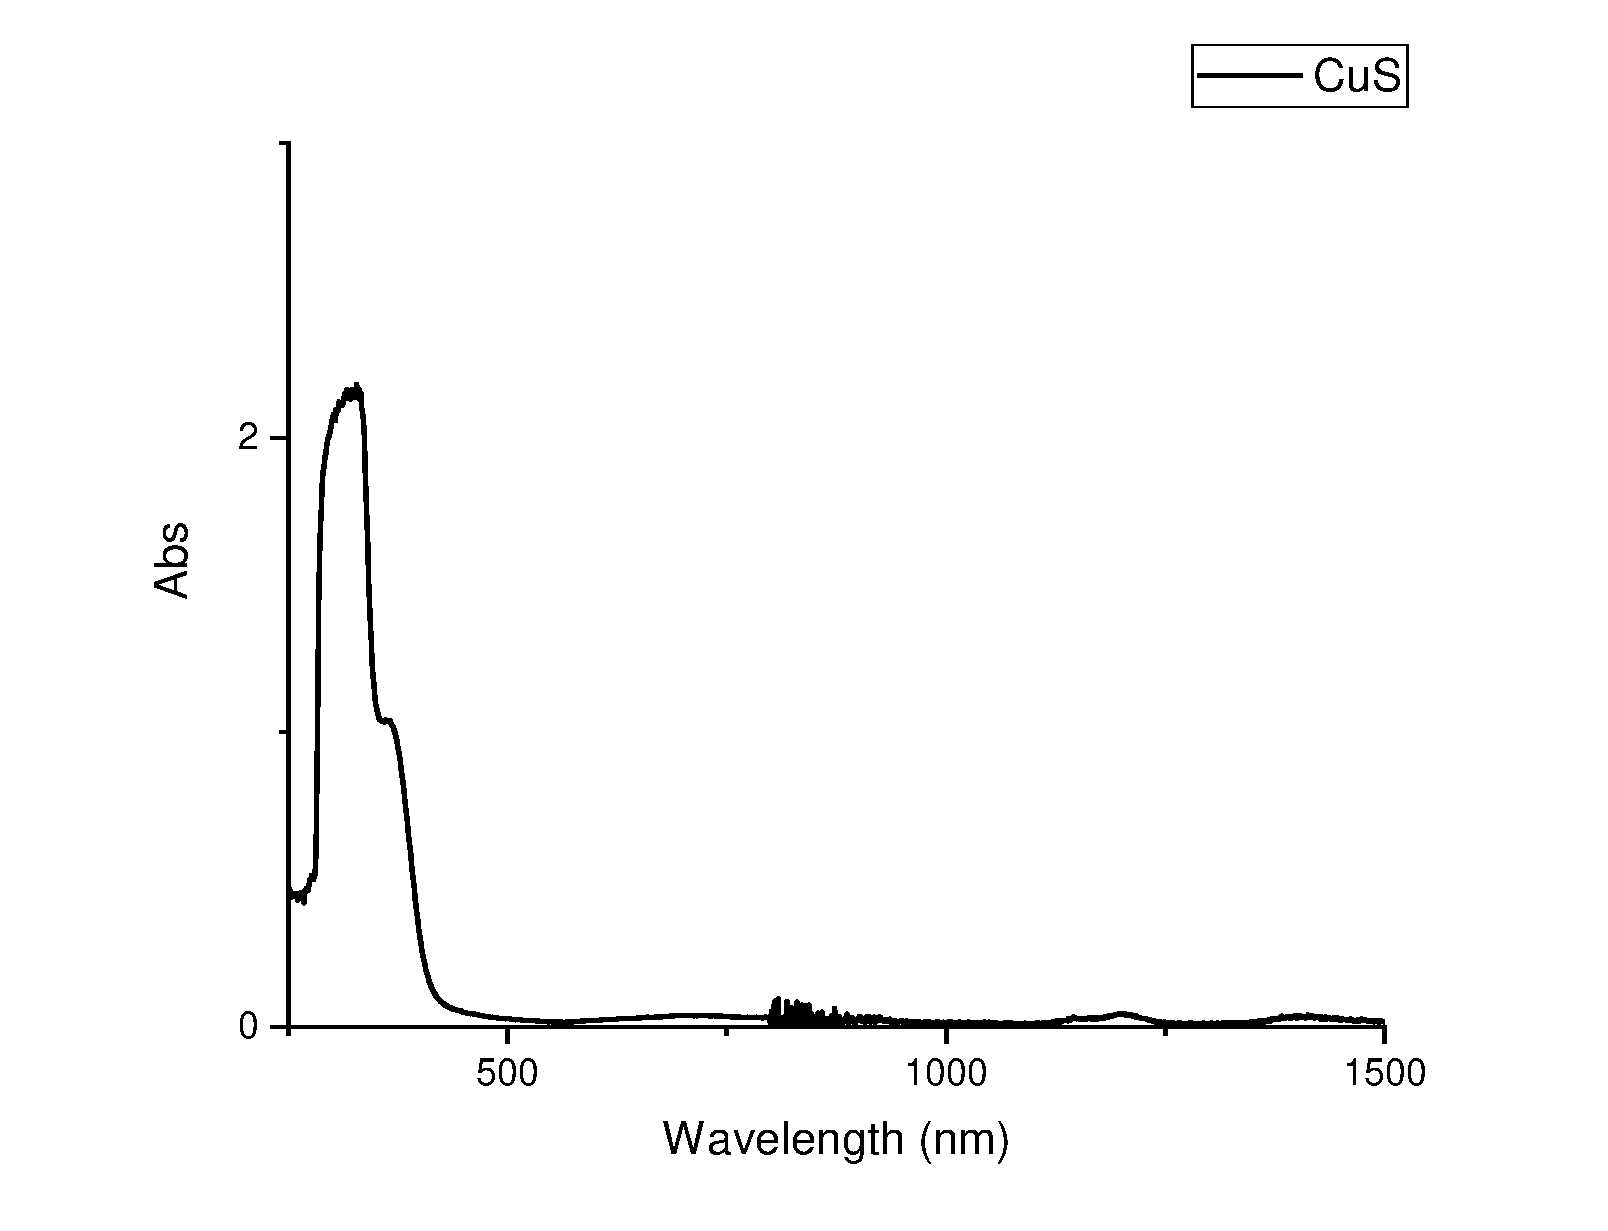
\includegraphics[width=0.6\textwidth]{Bilder/UV-CuS} 	
		\caption{Absorptionsspektrum der CuS-Nanopartikel in Toluol, gemessen in einer Ulbrichtkugel.}
		\label{fig:UV-CuS}
	\end{figure}
	
	\begin{figure}[H]
		\centering
		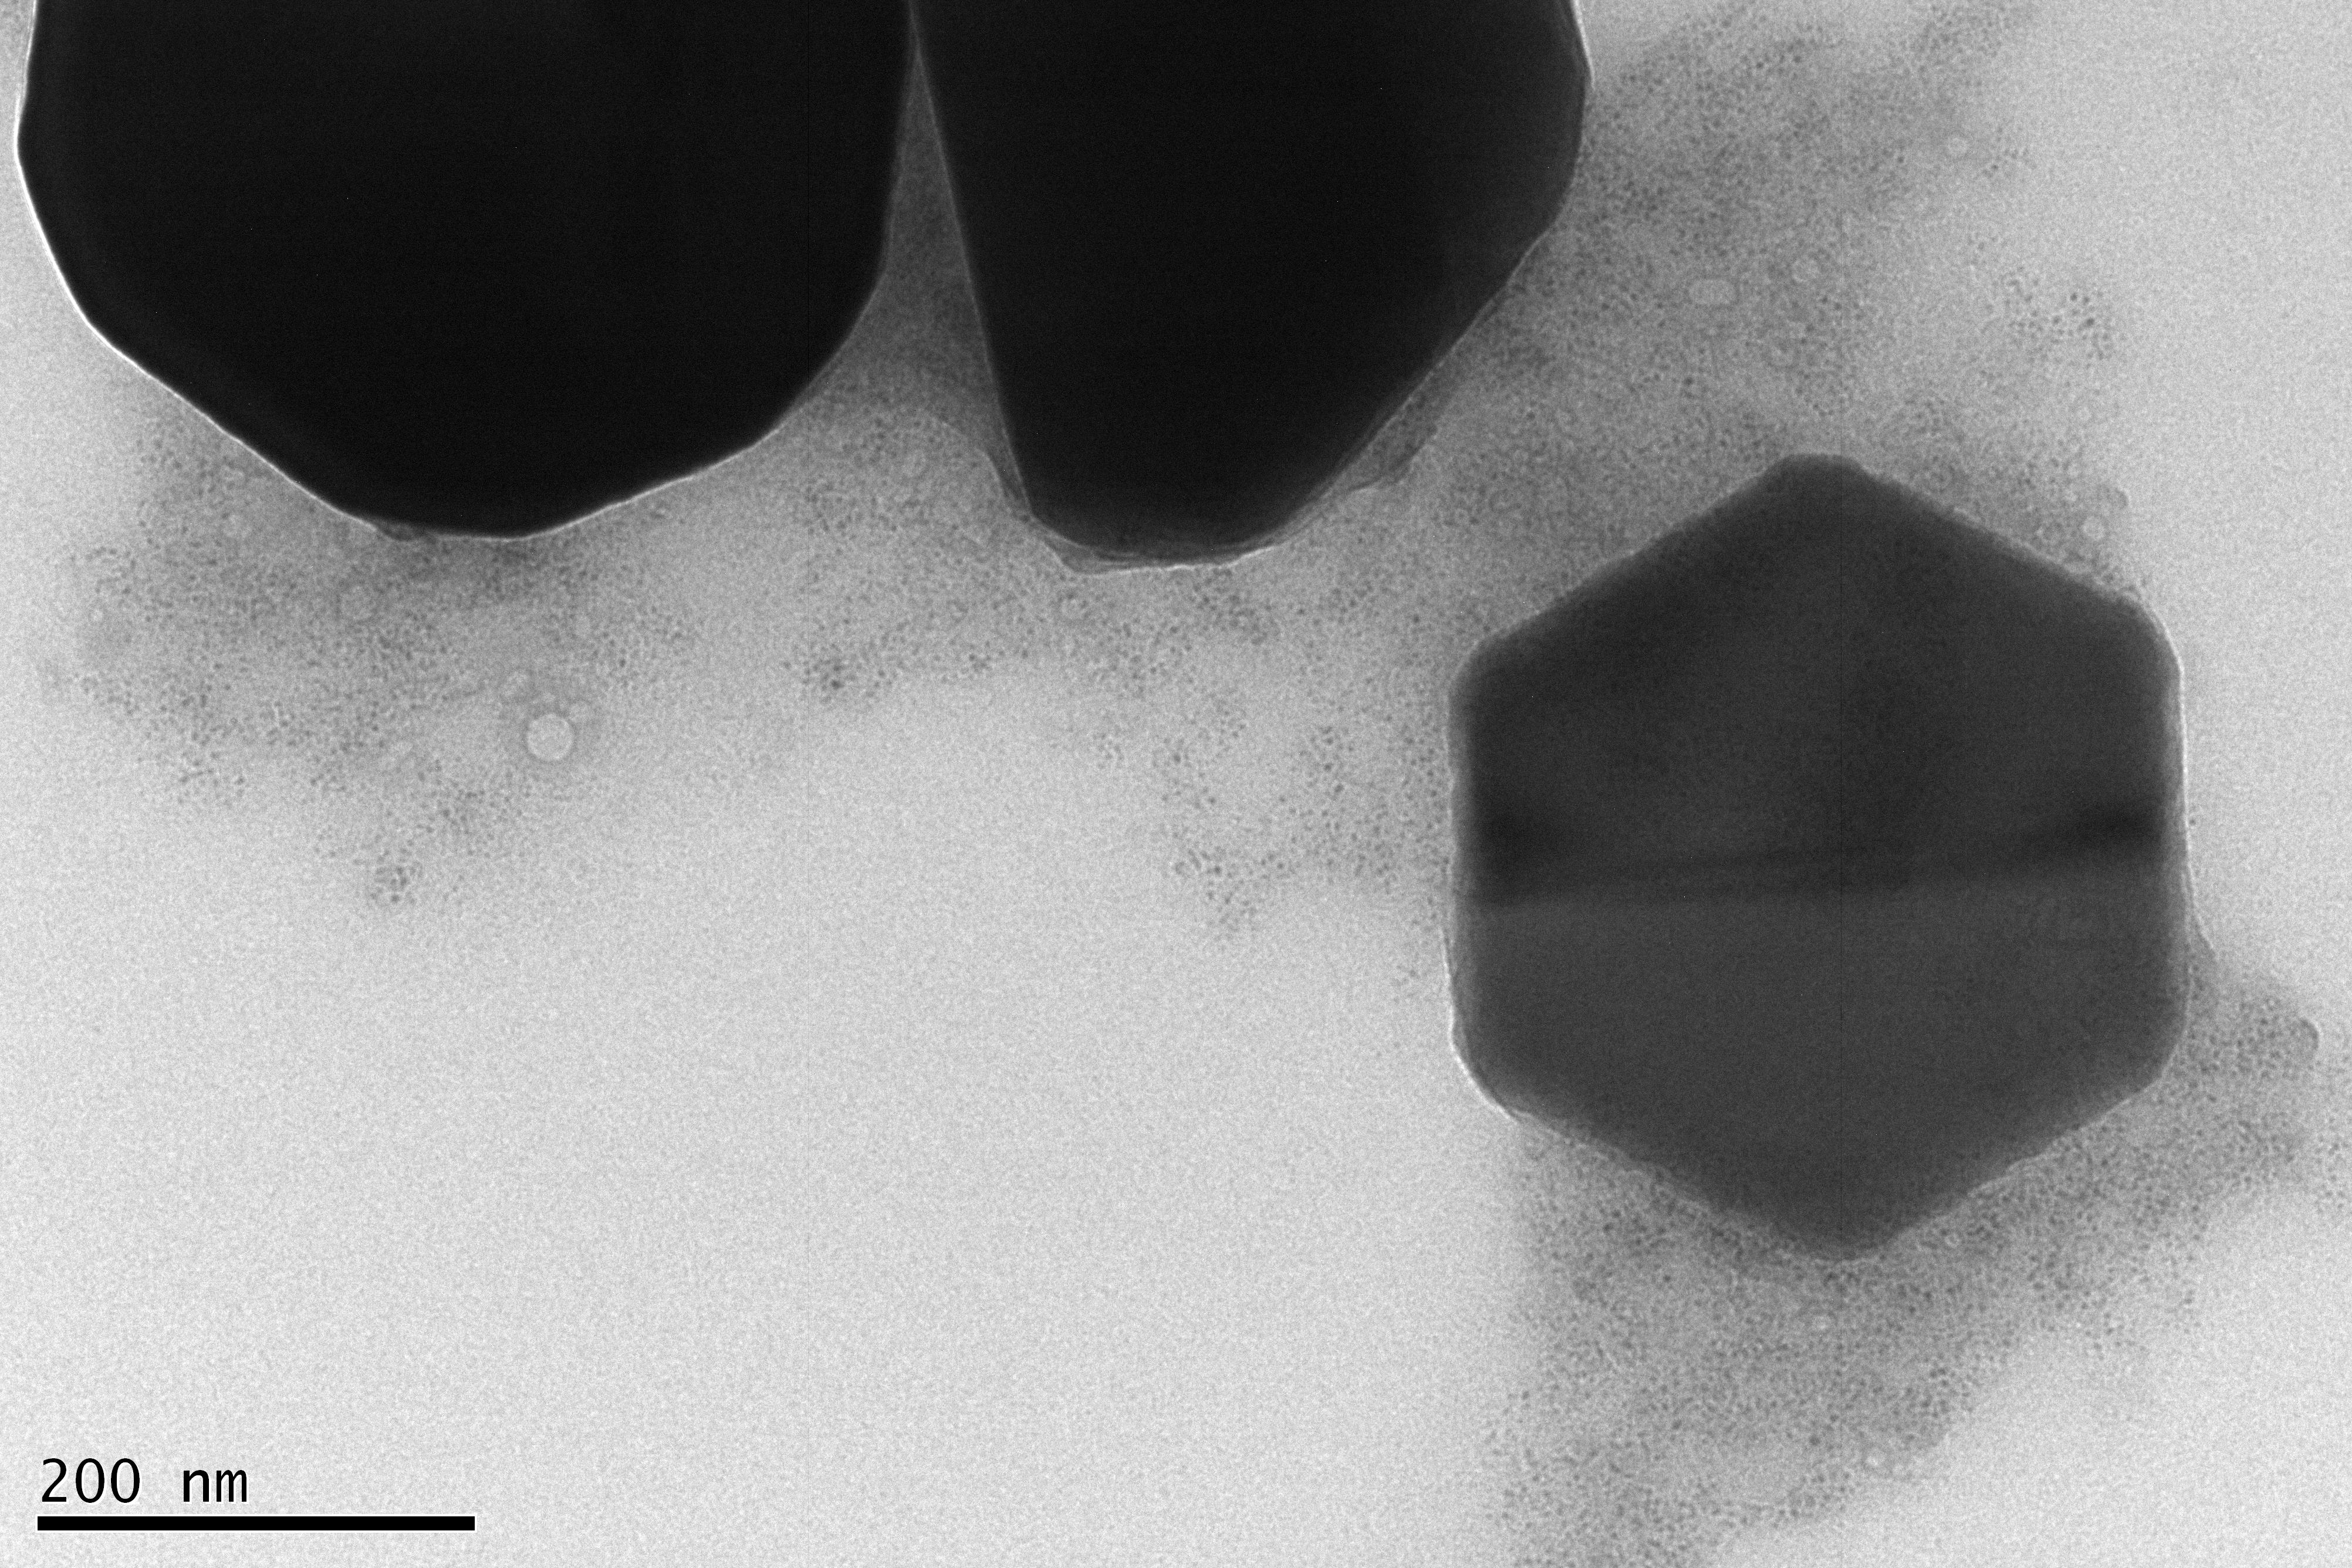
\includegraphics[width=0.6\textwidth]{Bilder/TEM-CuS} 	
		\caption{TEM-Bild der CuS-Nanopartikel.}
		\label{fig:TEM-CuS}
	\end{figure}
	
\subsection{Synthese Goldnanopartikel}
	Bei dieser Synthese war es das Ziel möglichst monodisperse Goldnanopartikel herzustellen.
	Die Partikel wurden per UV-vis-Spektroskopie und mit TEM untersucht.
	Das UV-vis zeigt ein für Gold typisches, durch LOPR bedingtes, Absorptionsmaximum von $\lambda_{Gold}$=\SI{519}{\nano\meter}, wie in \cref{fig:UV-AuNP} dargestellt.
	Aus den TEM-Bildern geht hervor, dass die Partikel eine mittlere Größe von etwa \SI{7,6}{\nano\meter} mit einer Abweichung von etwa \SI{0,6}{\nano\meter} besitzen, wie \cref{fig:TEM-Au-Hex-2} zeigt.	
	Die Partikel zeigten also eine zufriedenstellende Größenverteilung und können somit für weitere Experimente verwendet werden.
	
	\begin{figure}[H]
		\centering
		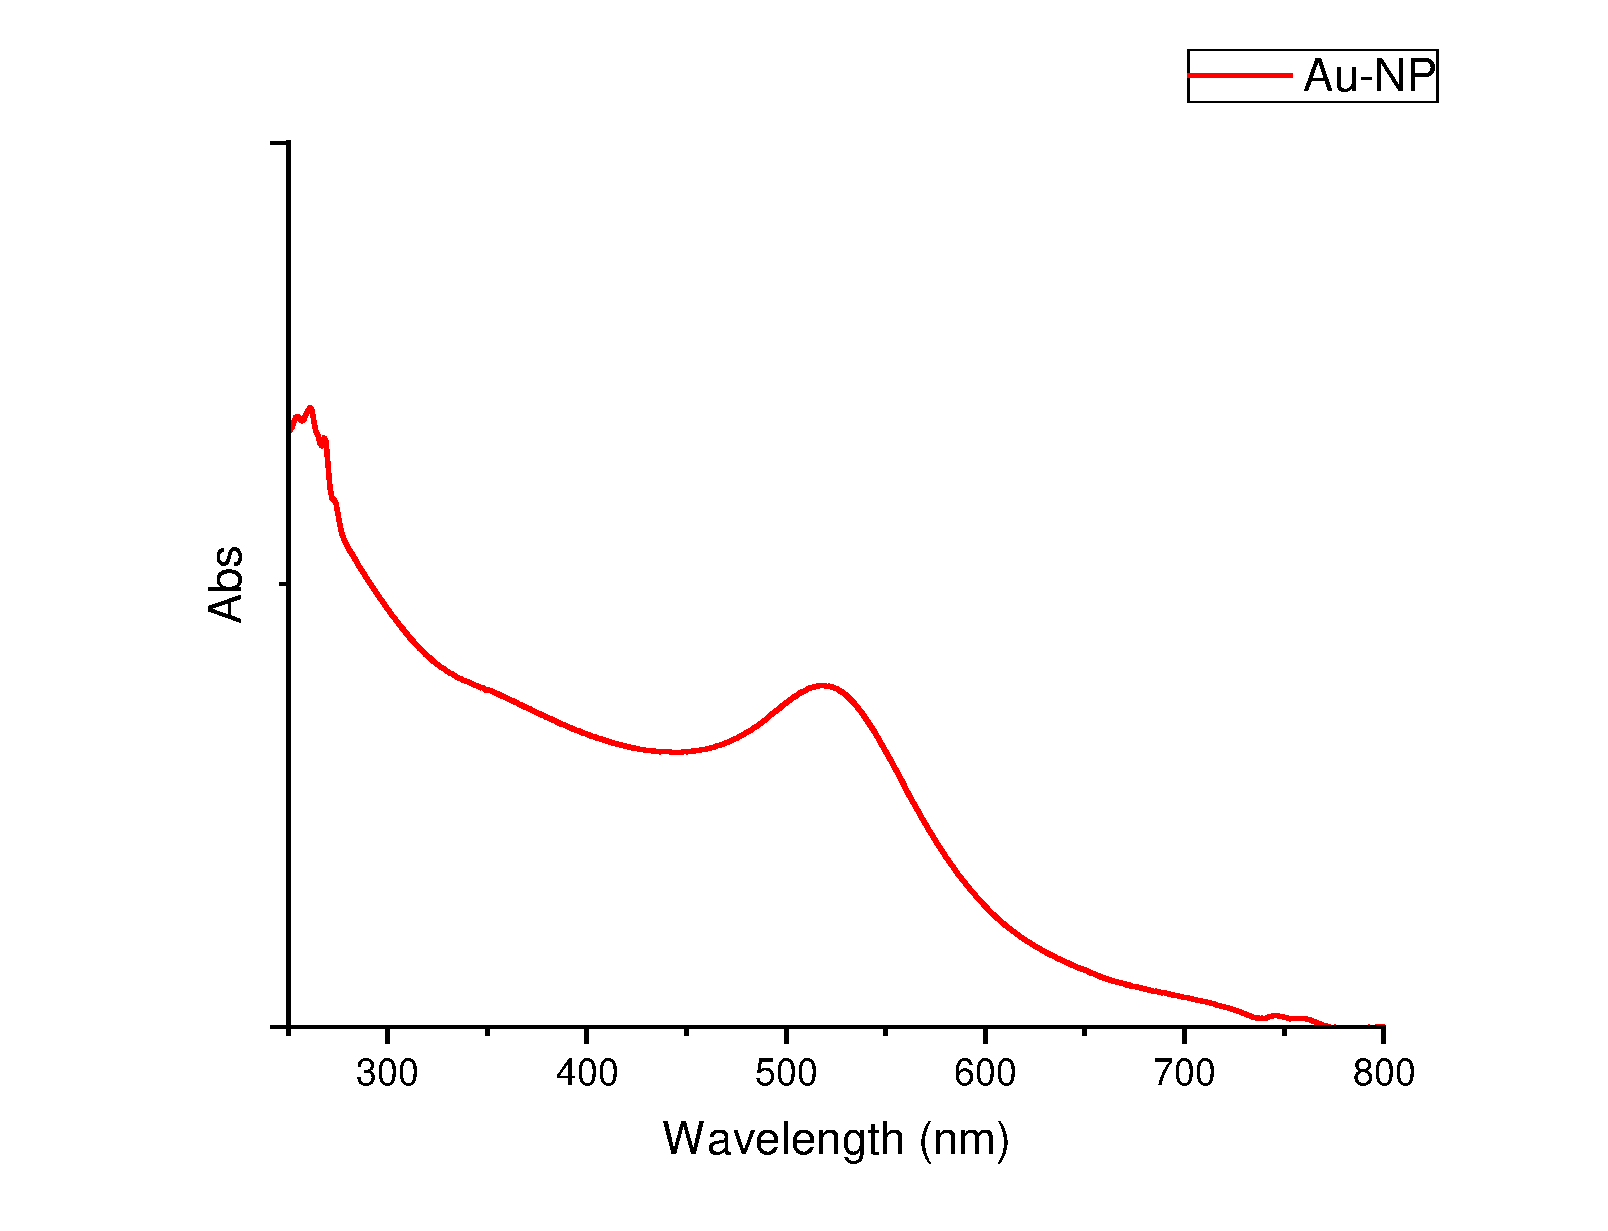
\includegraphics[width=0.6\textwidth]{Bilder/Gold-NP-Organisch} 	
		\caption{Absorptionsspektrum der Goldnanopartikel in Hexan gemessen.}
		\label{fig:UV-AuNP}
	\end{figure}
	
	\begin{figure}[H]
		\centering
		\subfloat[\label{fig:TEM-Au-Hex}]{%
			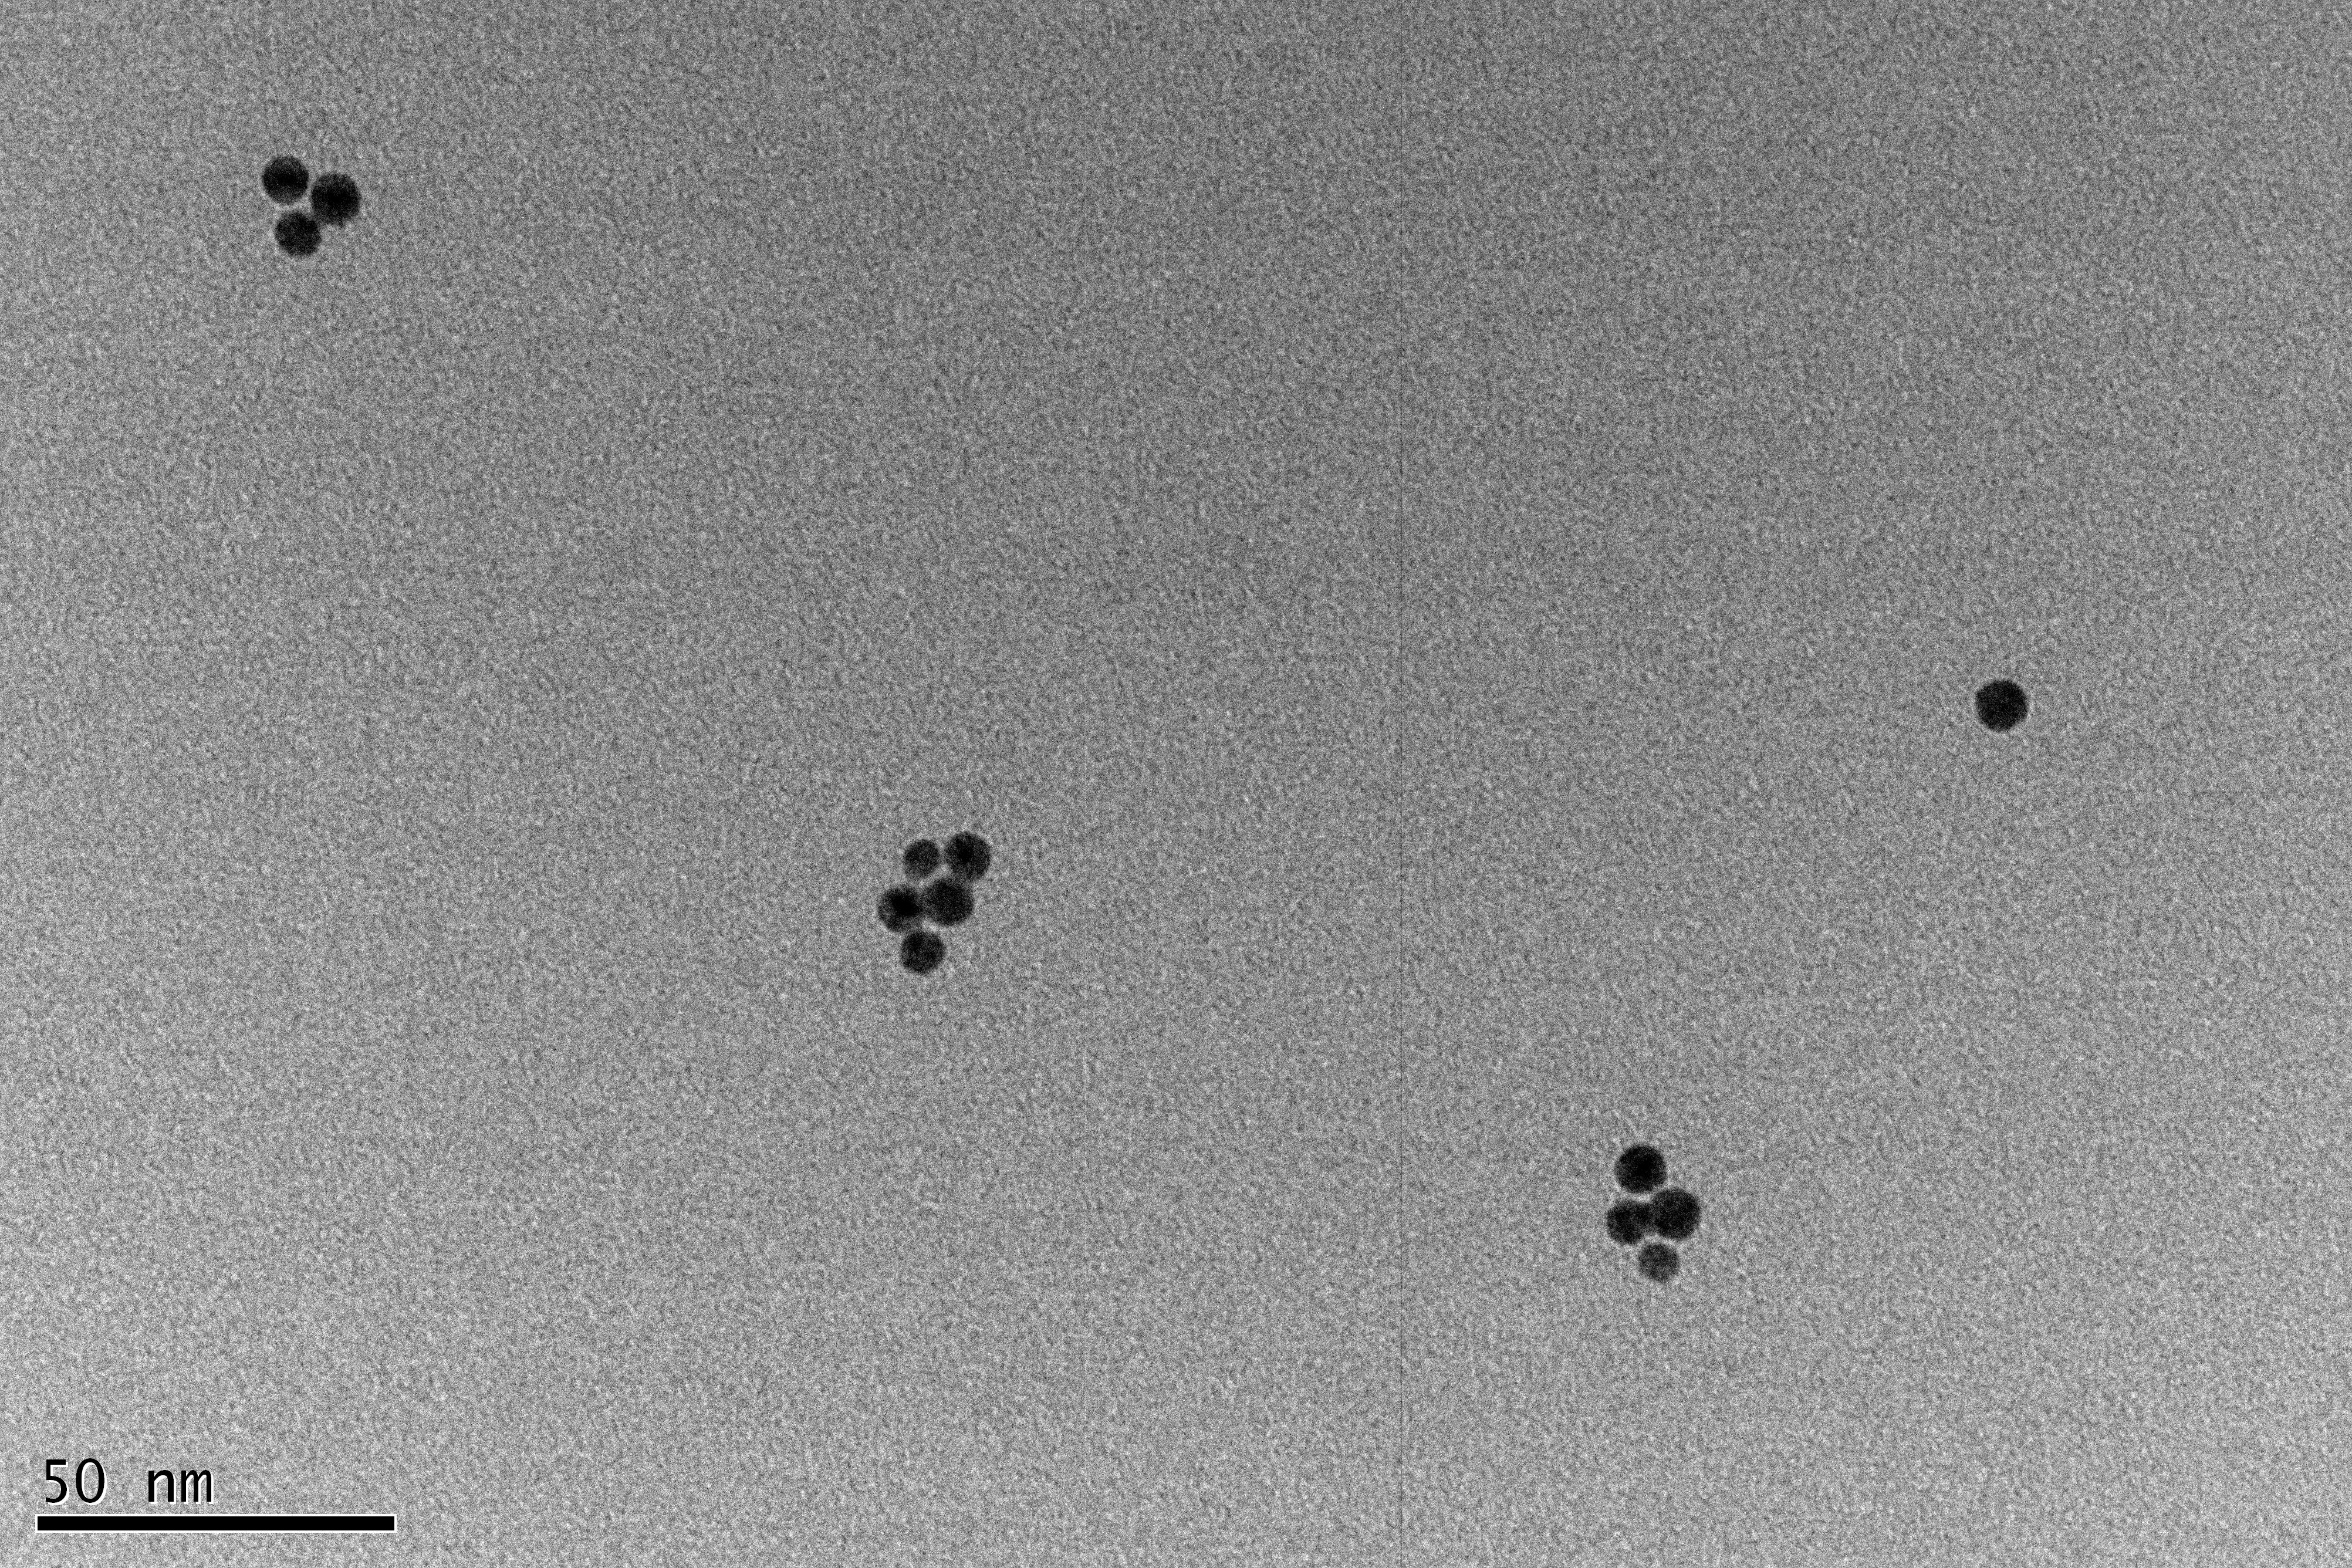
\includegraphics[width=0.45\linewidth]{Bilder/TEM-Au-Hex}}
		\subfloat[\label{fig:Size-Gold-NP}]{%
			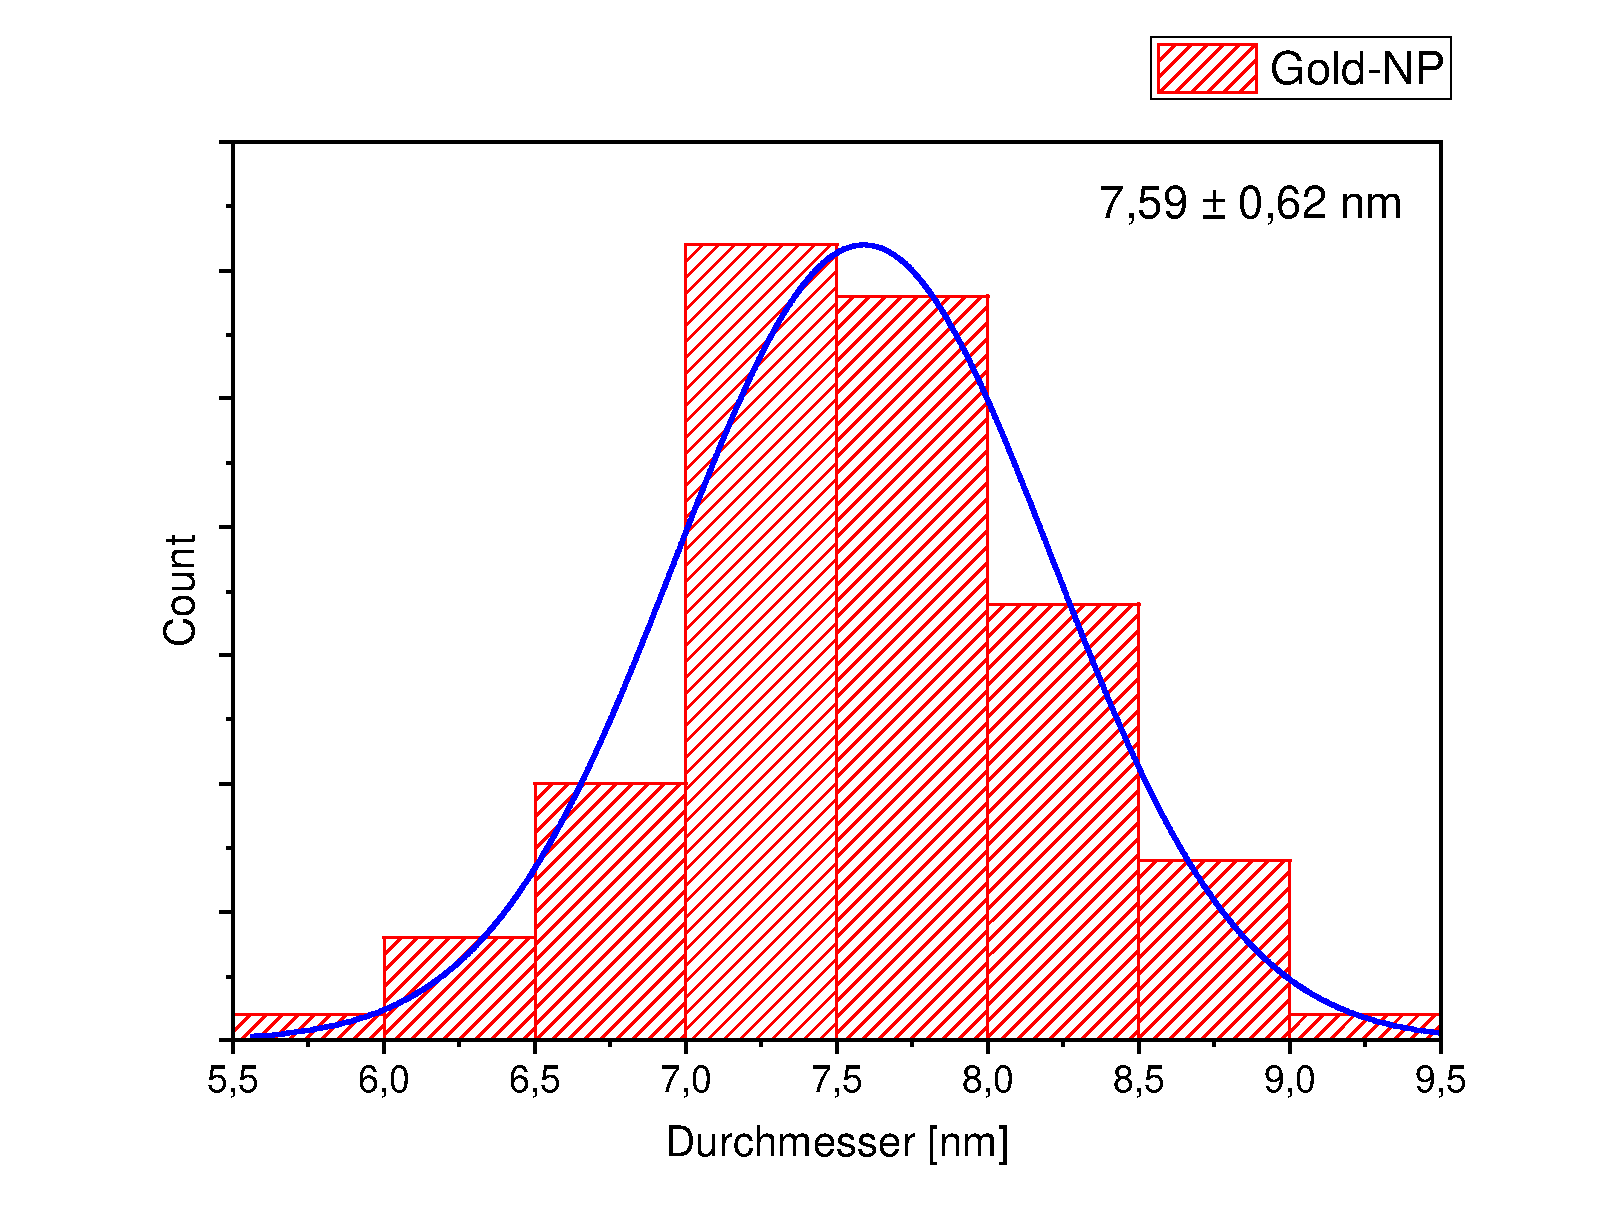
\includegraphics[width=0.45\linewidth]{Bilder/Size-Gold-NP-Organisch}}
		\caption{\emph{(a)}: TEM-Aufnahme der Gold-NP und \emph{(b)}: Größenverteilung.}
		\label{fig:TEM-Au-Hex-2}
	\end{figure}

	

	
	
\subsection{Synthese von CuS mit \ch{Cu[DDTC]2} und \ch{CuCl2}}
	
	Neben der CuS-Synthese aus reinem \ch{Cu[DDTC]2} wurde auch der Einfluss von Chloridionen auf die Partikelbildung untersucht, indem ein Teil des \ch{Cu[DDTC]2} durch \ch{CuCl2} ersetzt wurde.
	 
	Bei der Synthese von \ch{Cu[DDTC]2} und \ch{CuCl2} zeigt sich deutlich der Einfluss des \ch{CuCl2}. 
	Während bei reinem \ch{Cu[DDTC]2} die Partikel auf eine Größe von über \SI{300}{\nano\meter} wachsen und es dementsprechend wenig Partikel gibt, zeigen die TEM-Aufnahmen, die in \cref{fig:TEM-CuCl} gezeigt sind, dass es hier zu vielen kleinen Partikeln in der Größe von Quantenpunkten kommt, was darauf hinweist, dass das Chlorid als Ligand wirkt, das die kleineren Partikel stabilisiert.
	
	\begin{figure}[H]
		\centering
		\subfloat[\label{fig:CuCl-1}]{%
		\includegraphics[width=0.45\linewidth]{Bilder/CuCl-1}}
		\subfloat[\label{fig:CuCl-2}]{%
		\includegraphics[width=0.45\linewidth]{Bilder/CuCl-2}}	
		\caption{TEM-Bilder von CuS-Nanopartikel, aus einem Gemisch von 80\% \ch{Cu[DDTC]2} und 20\% \ch{CuCl2}.}
		\label{fig:TEM-CuCl}
	\end{figure}
	
\subsection{Synthese von Kupfersulfid in Anwesenheit von Goldnanopartikeln}

	Um das Nukleationsverhalten bei der CuS-Synthese zu Untersuchen, wurde diese Reaktion in Anwesenheit von Goldnanopartikeln in verschiedenen Verhältnissen untersucht.
	Es wurden von diesen Mischungen jeweils UV-vis-NIR-Absorptionsmessungen vorgenommen und von ausgewählten Proben TEM-Aufnahmen und XRD-Messungen vorgenommen.
	
	\begin{figure}[H]
		\centering
		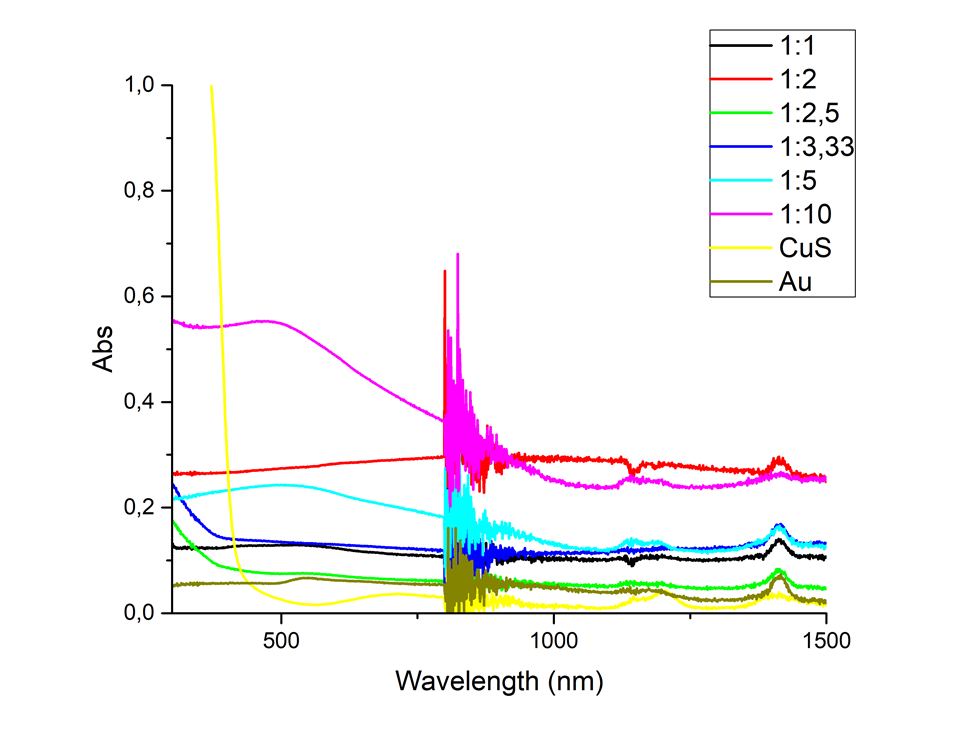
\includegraphics[width=0.6\textwidth]{Bilder/UV-AuCu-Konz} 	
		\caption{UV-vis-NIR-Messungen der Proben mit verschieden Mischungsverhältnissen von Au:\ch{Cu[DDTC]2} in Toluol (gemessen in Ulbrichtkugel).}
		\label{fig:UV-AuCu}
	\end{figure}
	
	Die Absorptionsmessungen in \cref{fig:UV-AuCu} zeigen, dass bei den Mischungen mit geringem Goldanteil ein Maximum bei etwa \SI{500}{\nano\meter} entsteht, dass mit steigendem Goldanteil abnimmt.
	Dies könnte das Plasmon der Goldpartikel sein.
	Interessanterweise ist das Maximum bei diesen Mischungen leicht blauverschoben und teilweise ausgeprägter als bei einer Vergleichsprobe, bei der die gleiche Reaktion ohne \ch{Cu[DDTC]2} und nur mit der Gold-NP-Lösung durchgeführt wurde.
	Zudem scheint das Plasmon bei einigen Proben stark verbreitert.
	Die Verschiebung des Plasmons könnte auf Größenänderungen der Goldpartikel oder  auf Veränderung der chemischen Umgebung zurückzuführen sein. 
	Die Verbreiterung des Plasmons weißt auf eine ungleiche Größenverteilung der Gold-Nanopartikel hin.
	
	Die TEM-Aufnahmen zeigen, dass bei den Proben sowohl mit einem hohen als auch bei einem niedrigen Au:\ch{Cu[DDTC]2}-Verhältnis es zu einzelnen kleinen Gruppen von Gold-Nanopartikeln kommt, die separat ohne gebildetes CuS in der Nähe vorliegen (\cref{fig:CuAu-10-10_2} bzw. \cref{fig:CuAu-10-1_2}).
	Bei geringem Goldanteil scheint ein Teil des \ch{Cu[DDTC]2} wie bei der Probe ohne Gold zu reinem hexagonalem CuS zu reagieren, wie \cref{fig:CuAu-10-1_3} zeigt.
	Insgesamt lässt sich hier aber erkennen, dass die CuS-Partikel in Anwesenheit von den Gold-NP sich deutlich anders ausbilden als bei reinem \ch{Cu[DDTC]2} und es an einigen Stellen so aussieht, als wären dort Goldpartikel eingelagert, was besonders in \cref{fig:CuAu-10-1_1} zu erkennen ist.
	
	\begin{figure}[H]
		\centering
		\subfloat[\label{fig:CuAu-10-10_1}]{%
			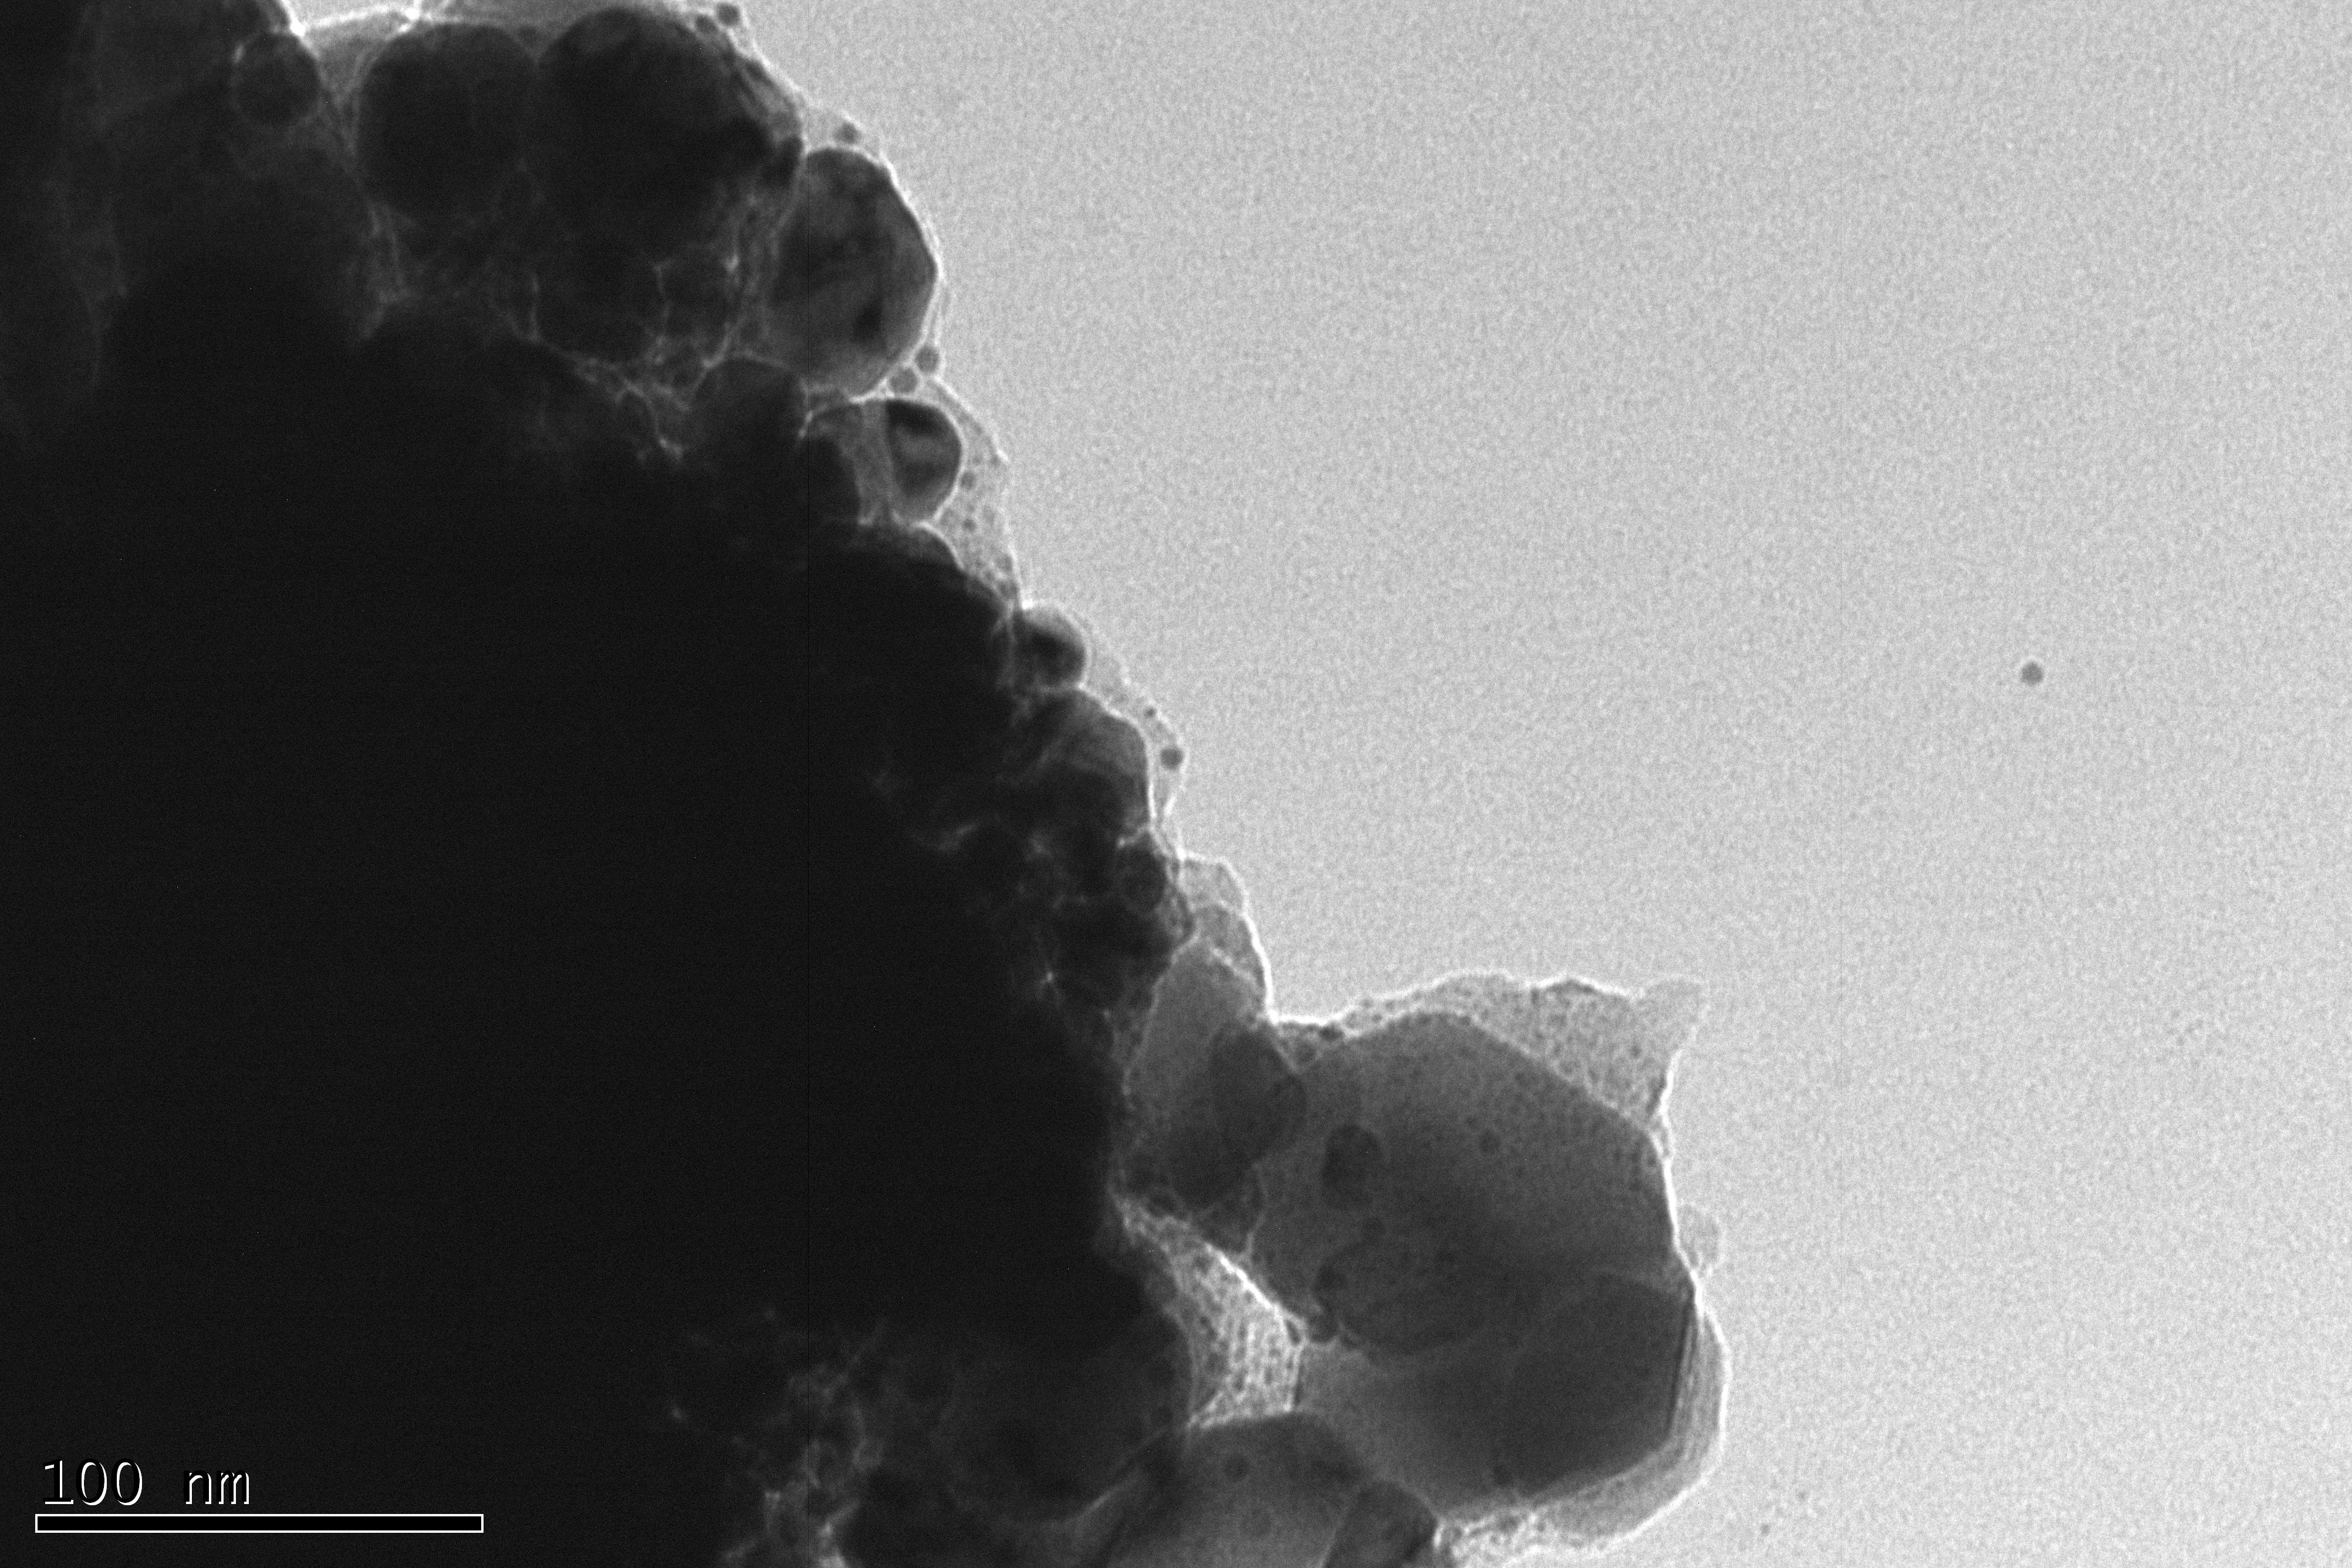
\includegraphics[width=0.33\linewidth]{Bilder/CuAu-10-10_1}}
		\subfloat[\label{fig:CuAu-10-10_2}]{%
			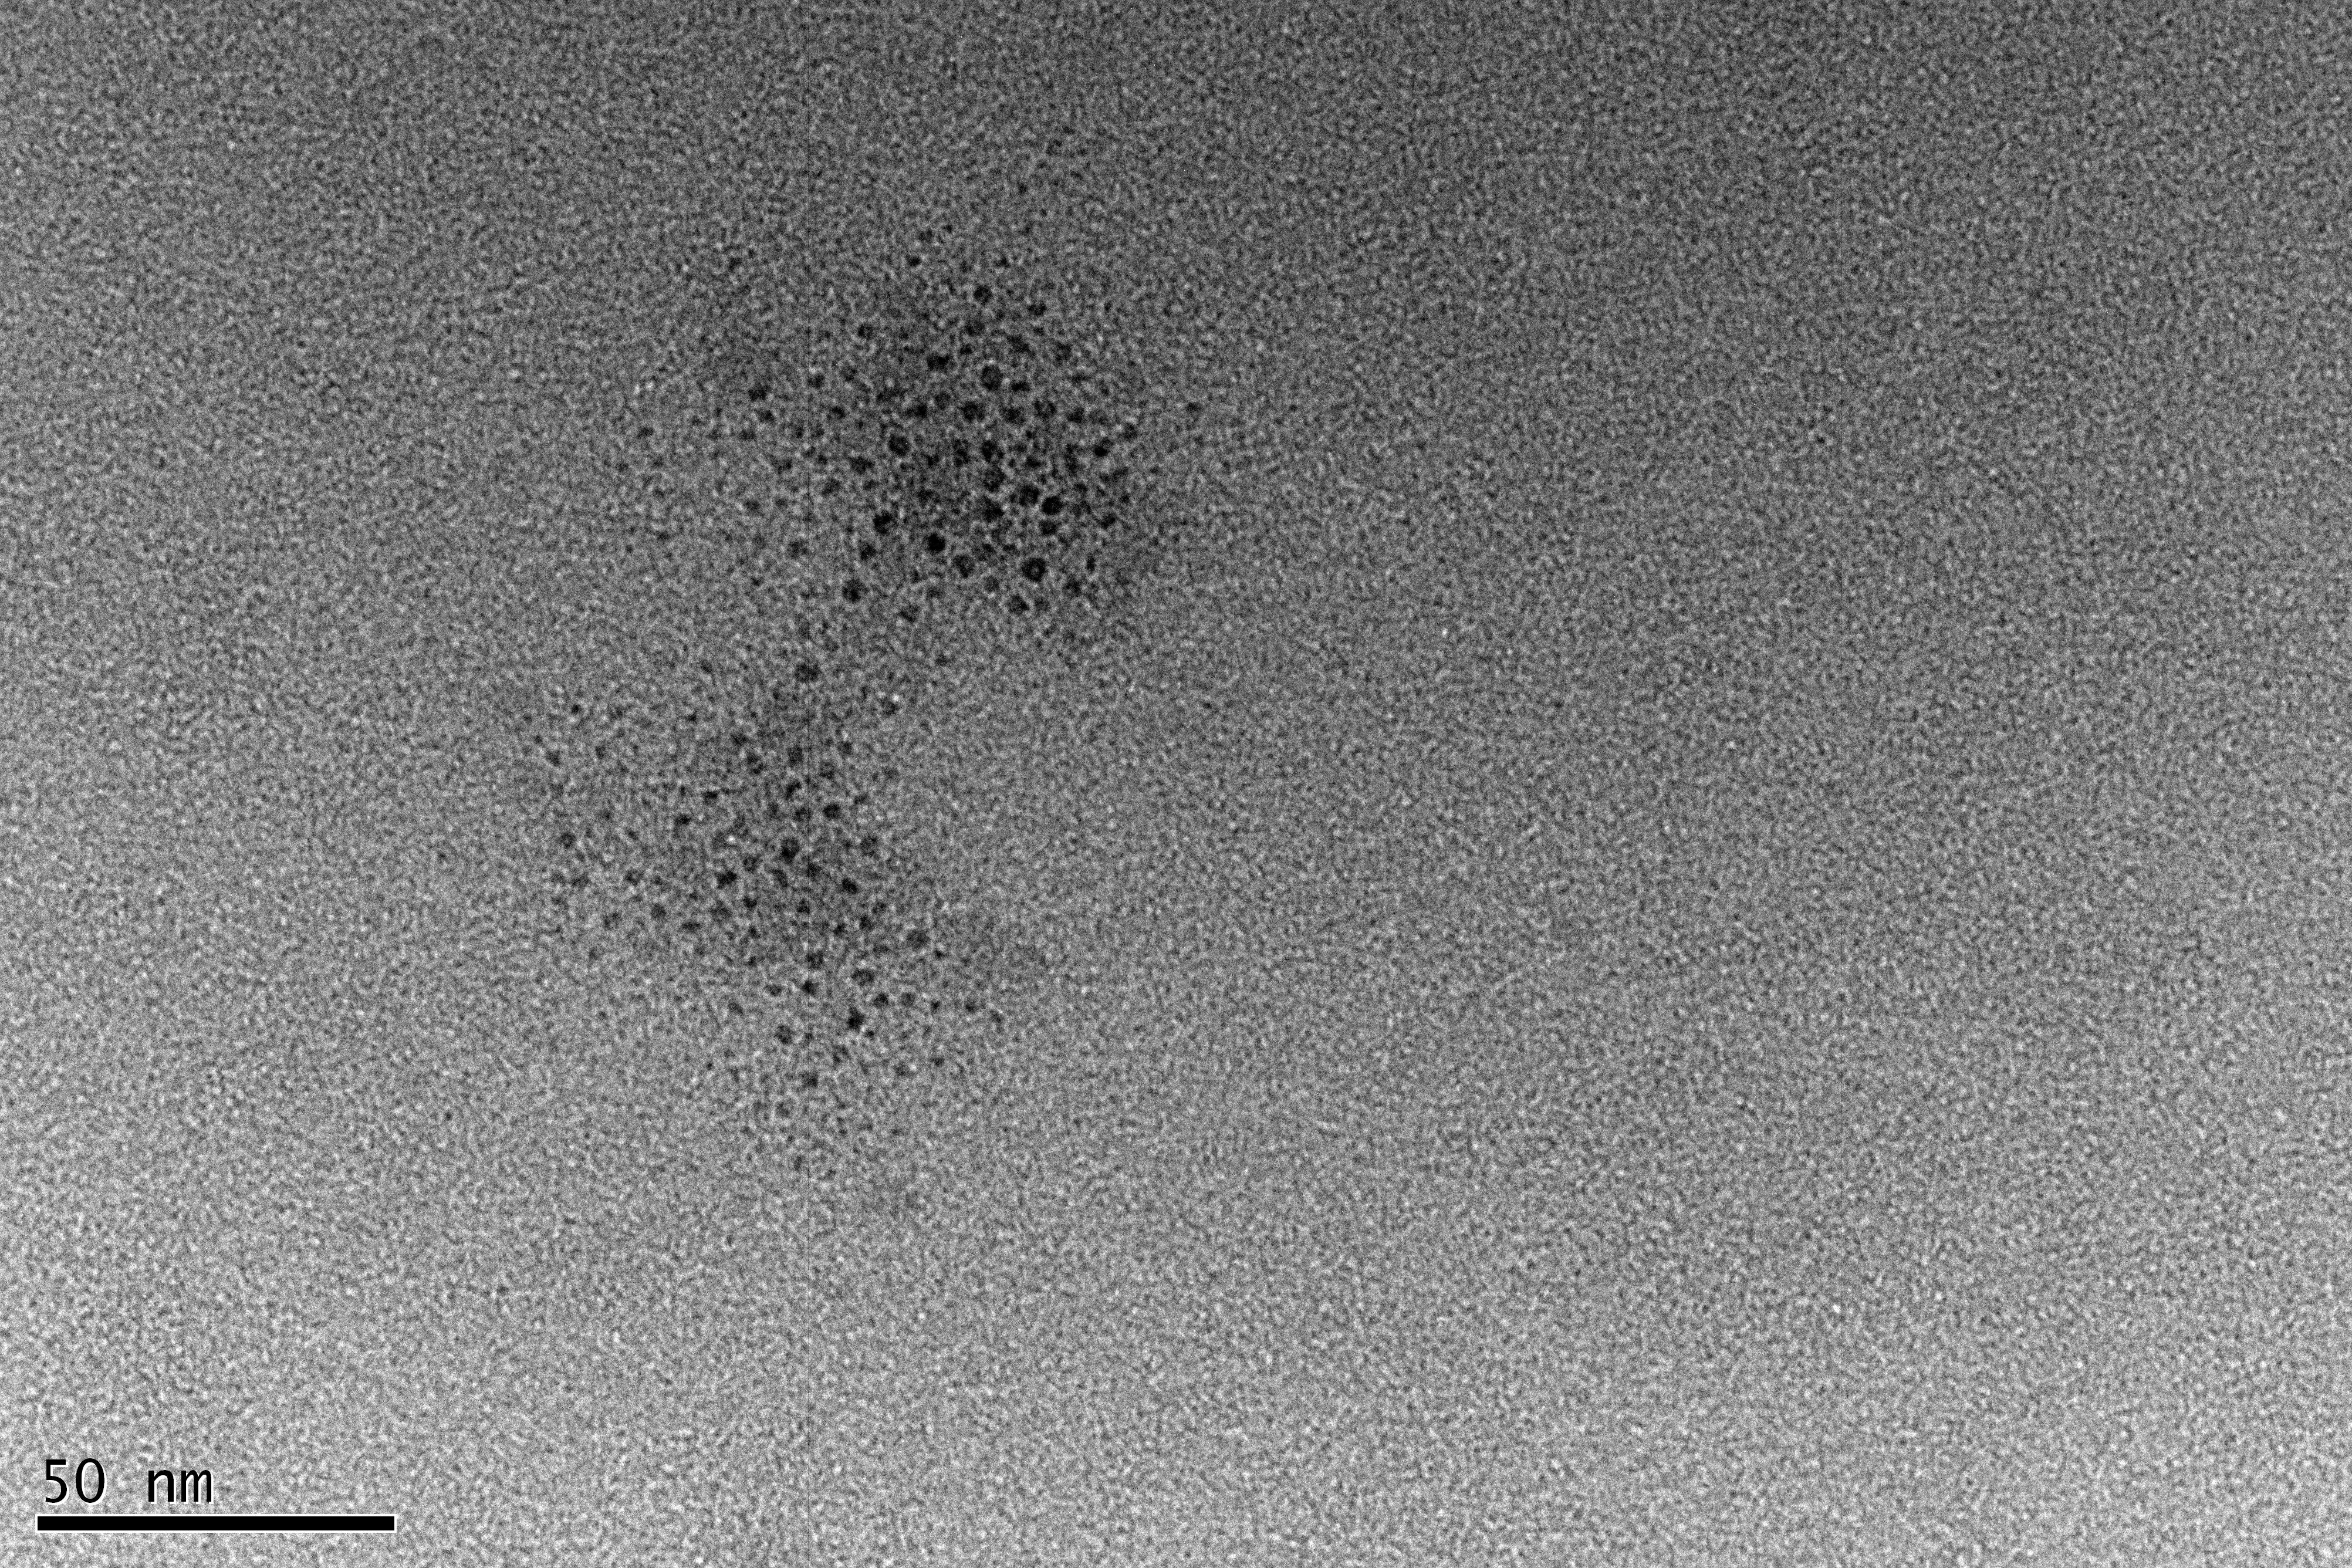
\includegraphics[width=0.33\linewidth]{Bilder/CuAu-10-10_2}}
		\subfloat[\label{fig:CuAu-10-10_3}]{%
			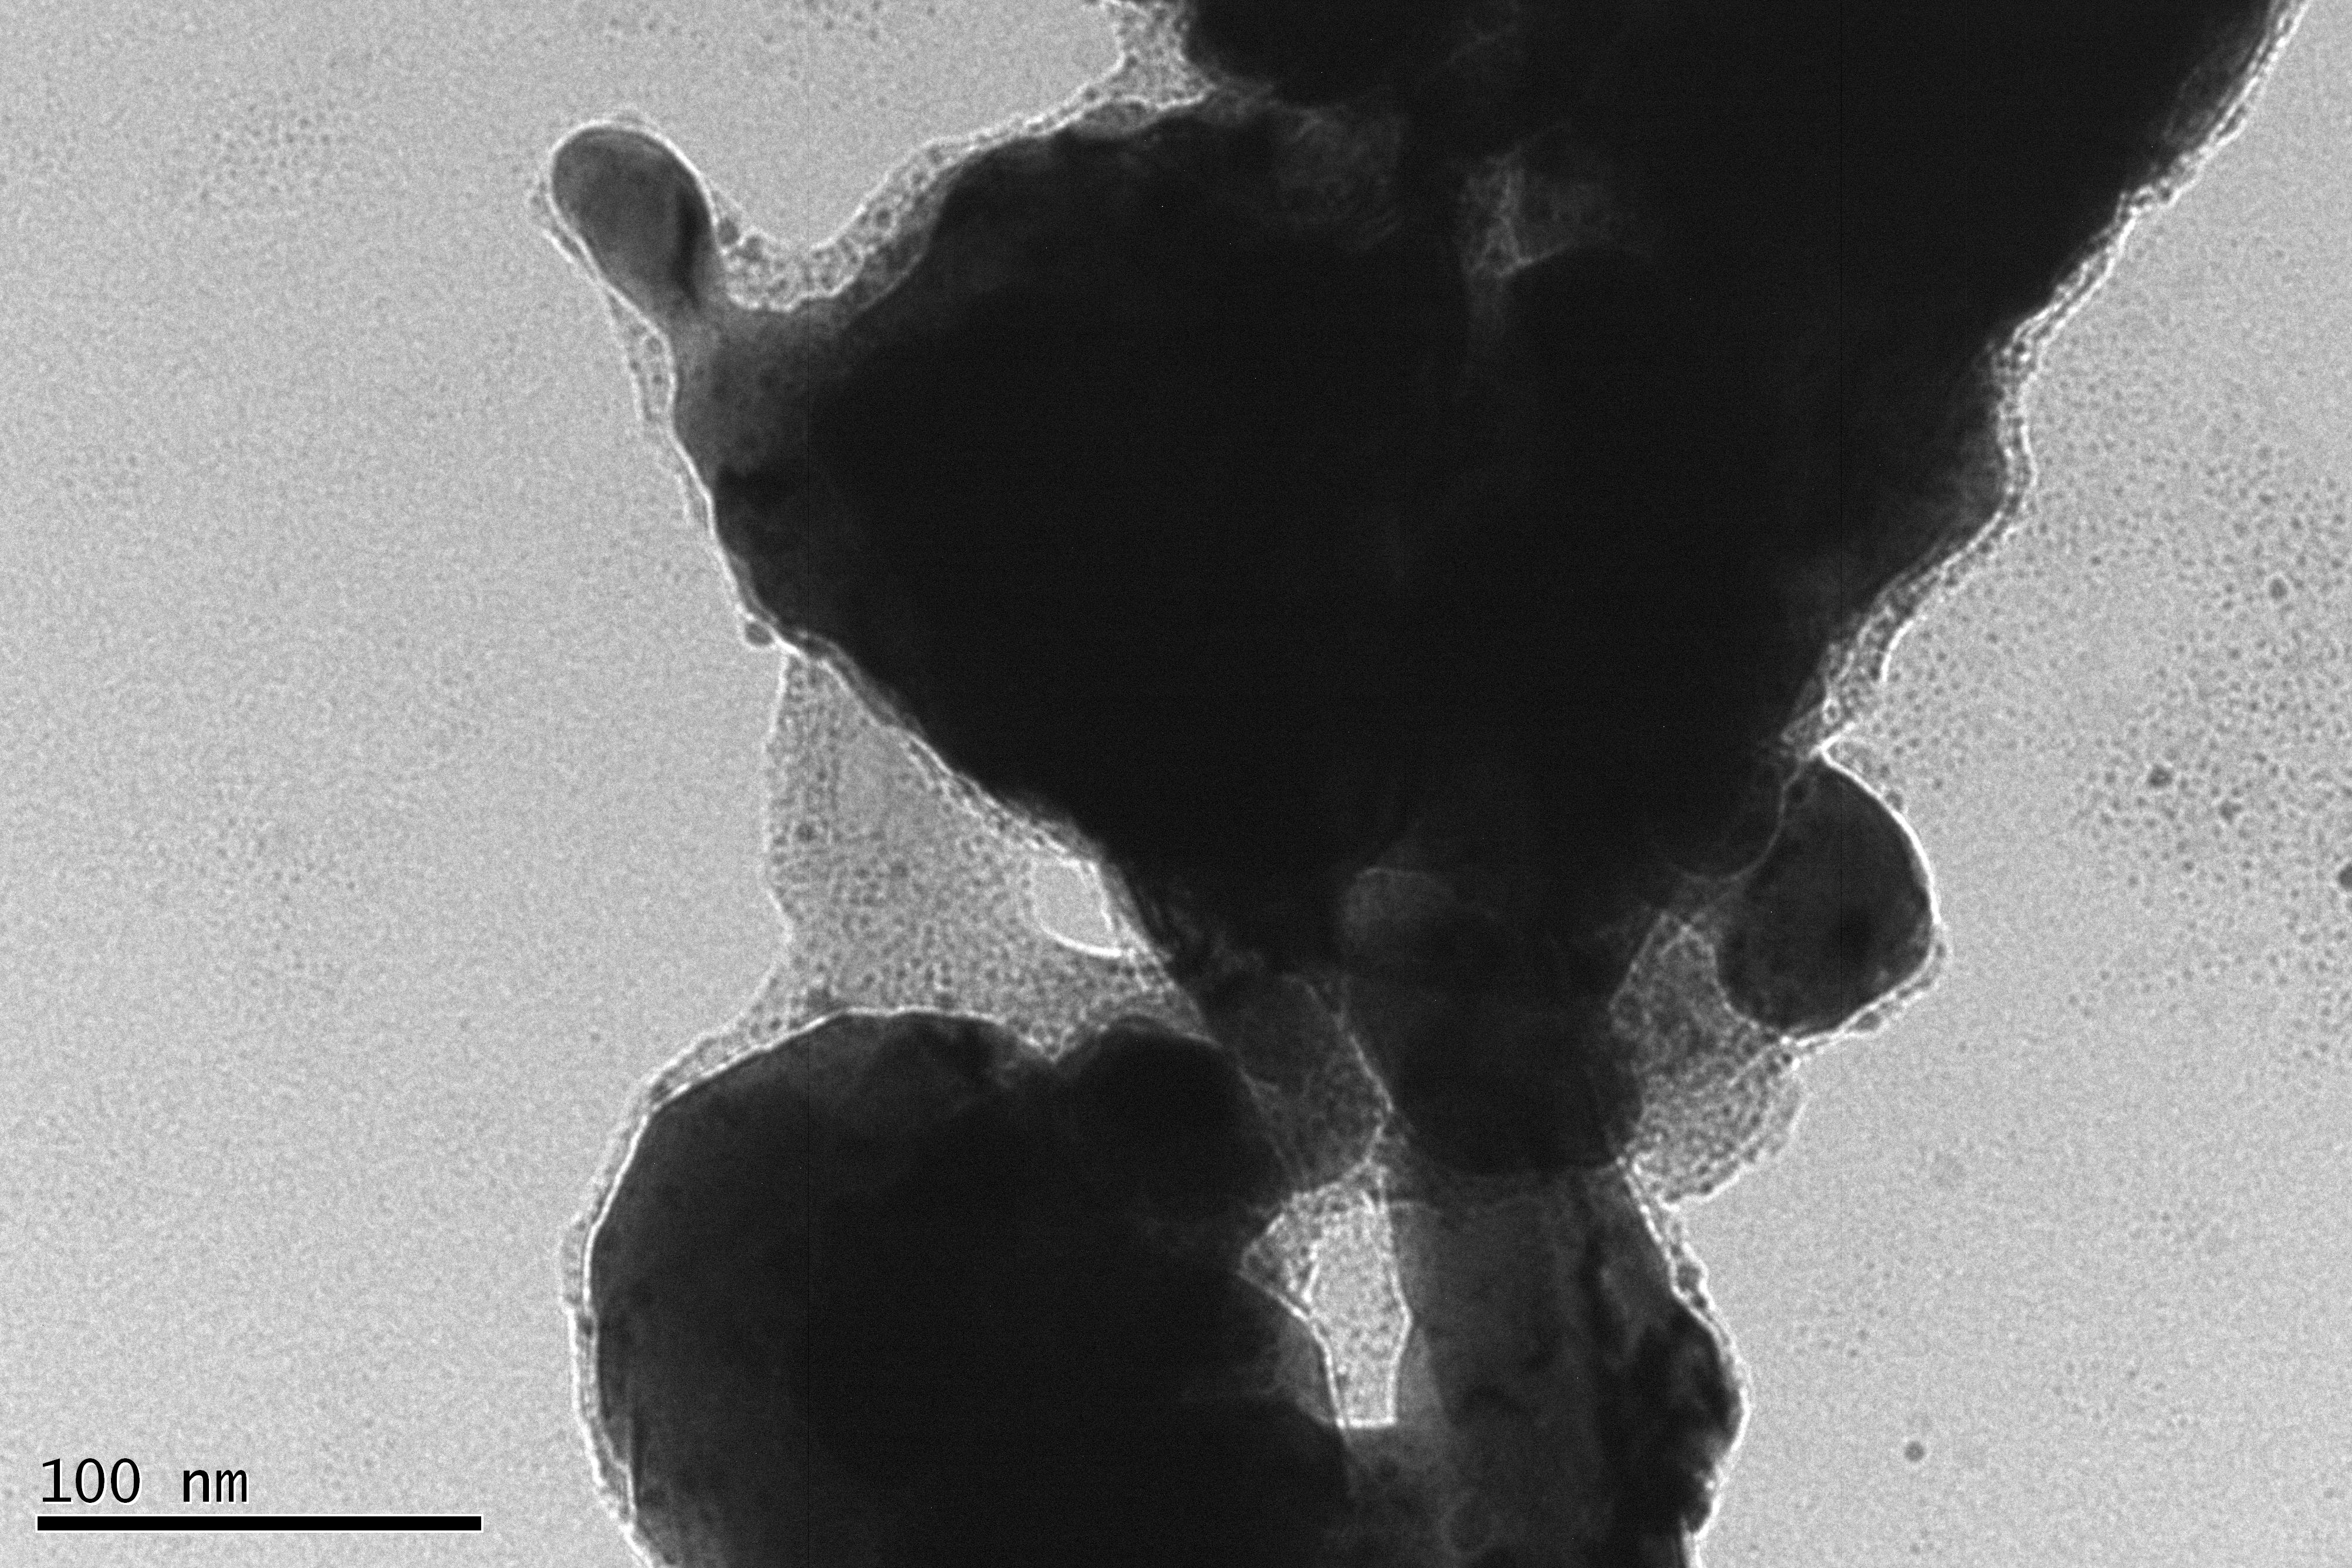
\includegraphics[width=0.33\linewidth]{Bilder/CuAu-10-10_3}}
		\caption{TEM-Aufnahmen der Probe mit einem Mengenverhältnis von 1:1 Au:\ch{Cu[DDTC]2}.}
		\label{fig:TEM-CuAu-10-10}
	\end{figure}
	
	\begin{figure}[H]
		\centering
		\subfloat[\label{fig:CuAu-10-1_1}]{%
			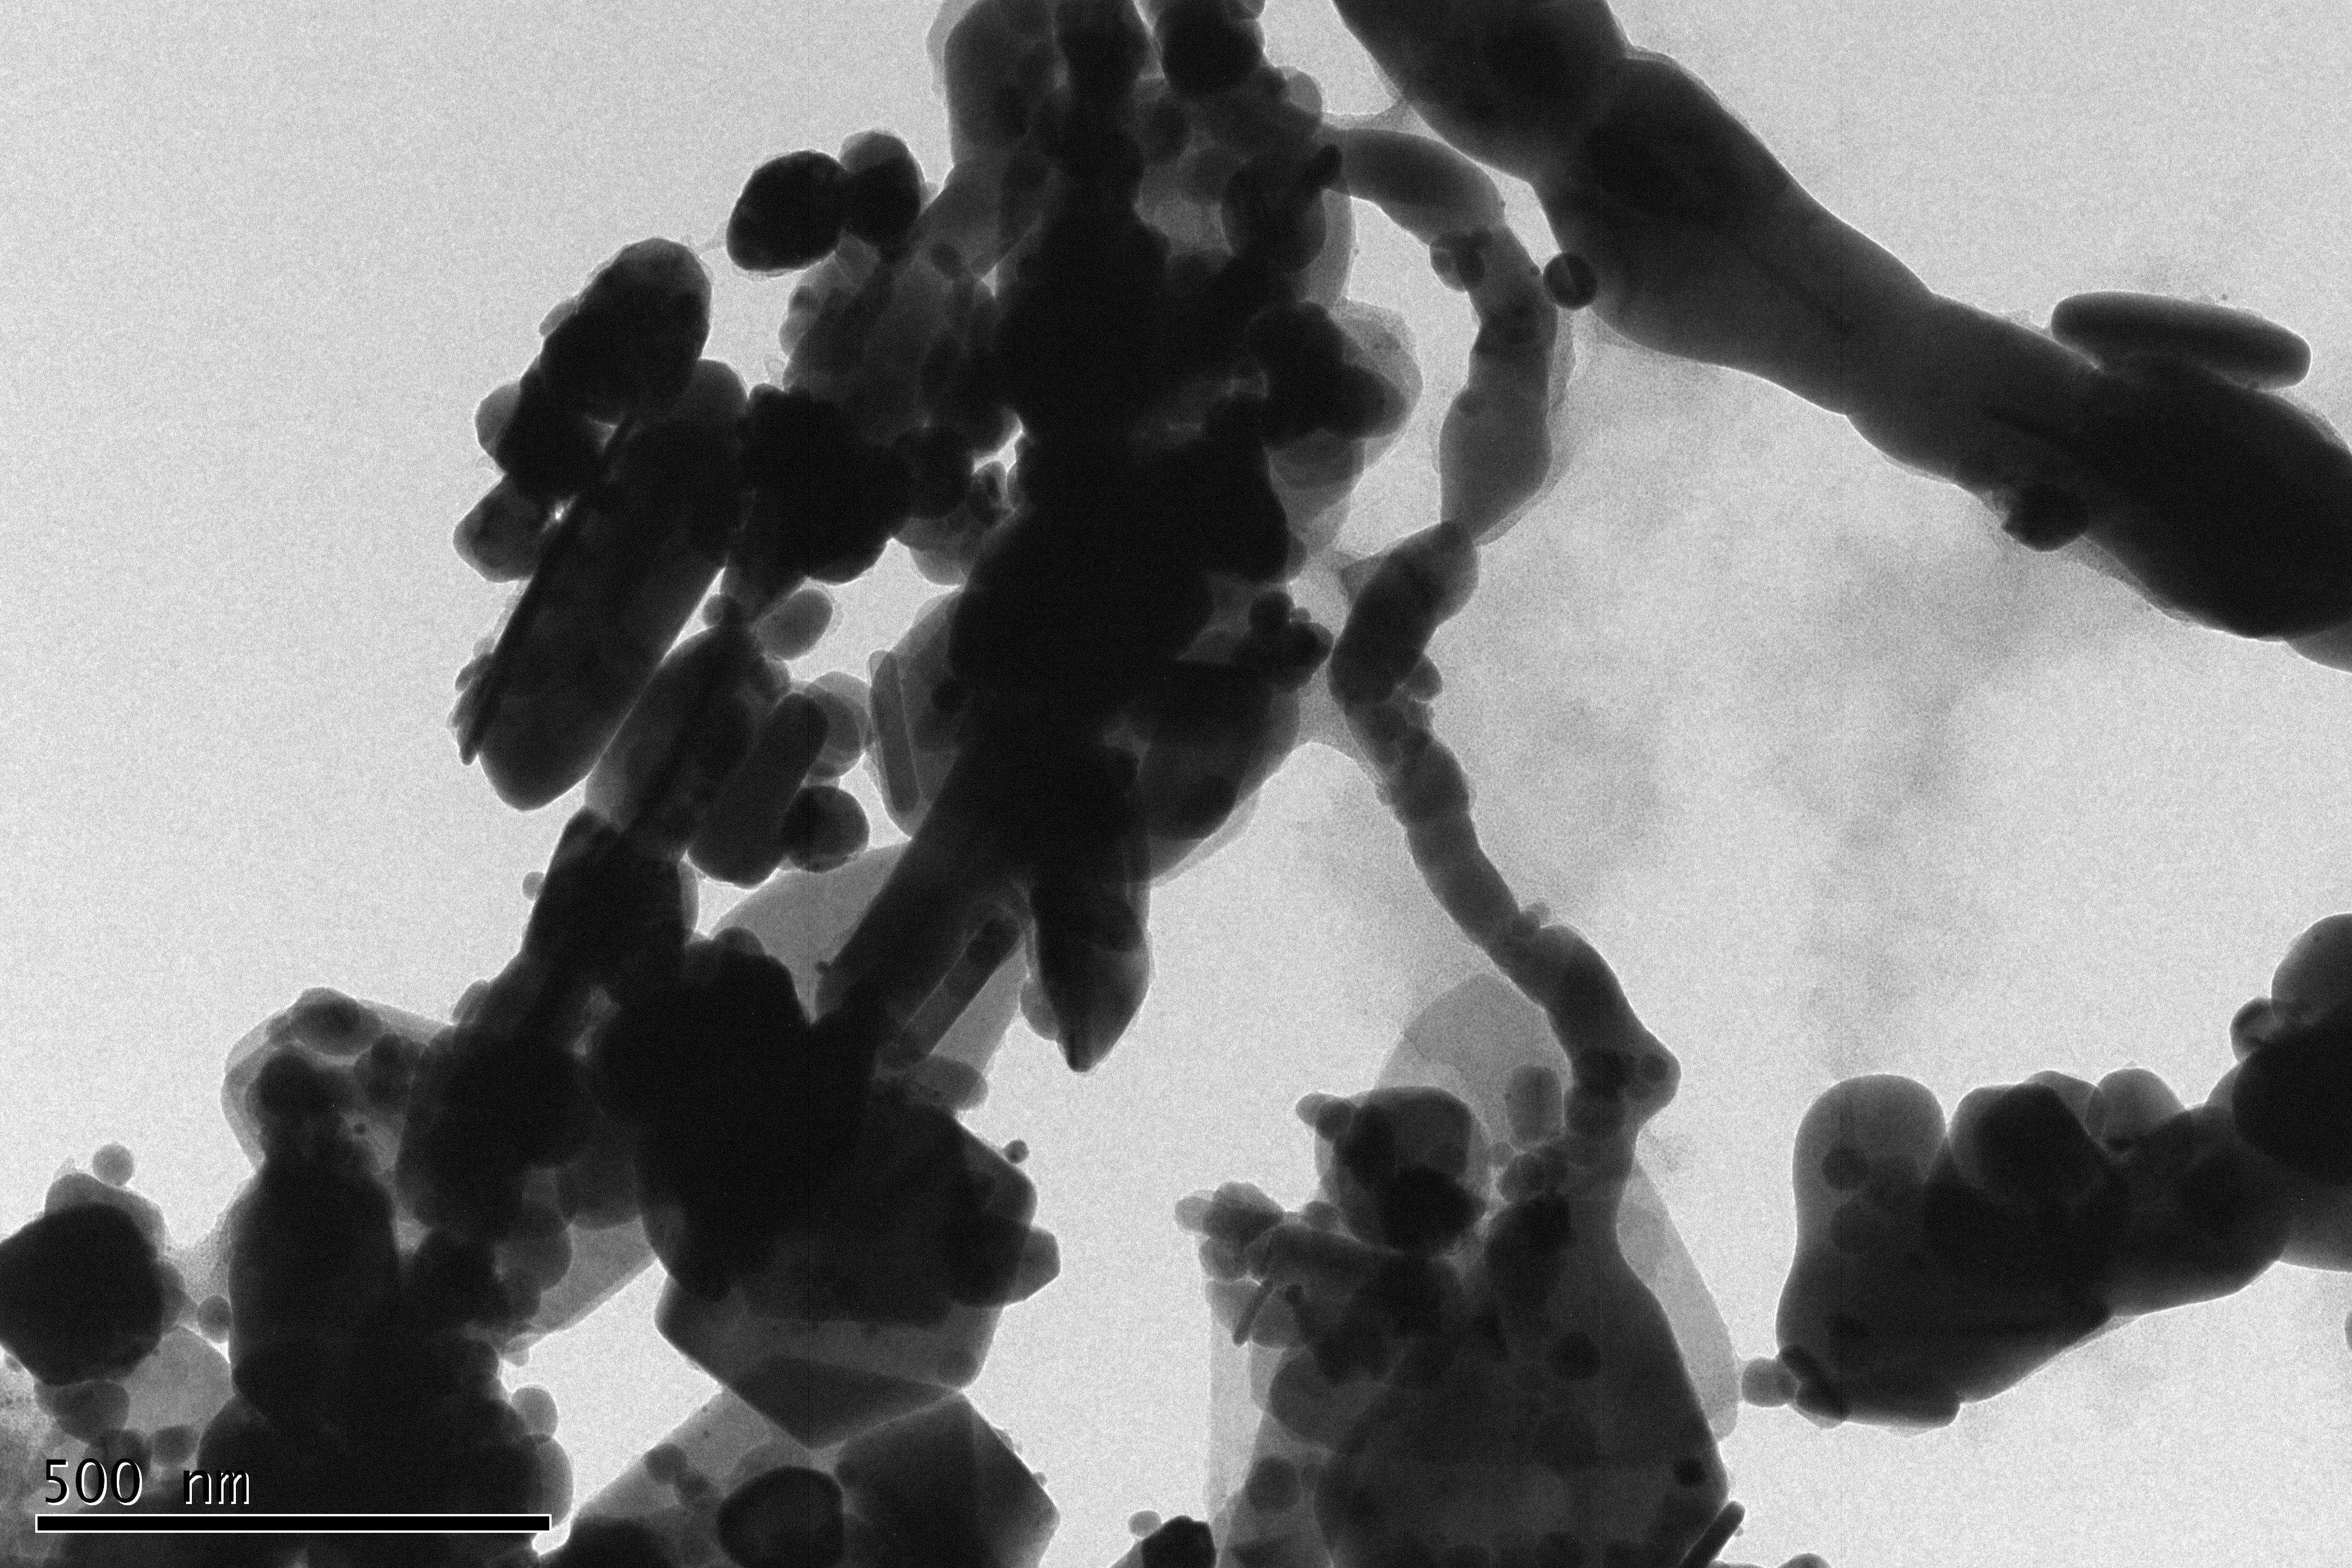
\includegraphics[width=0.33\linewidth]{Bilder/CuAu-10-1_1}}
		\subfloat[\label{fig:CuAu-10-1_2}]{%
			\includegraphics[width=0.33\linewidth]{Bilder/CuAu-10-1_2}}
		\subfloat[\label{fig:CuAu-10-1_3}]{%
			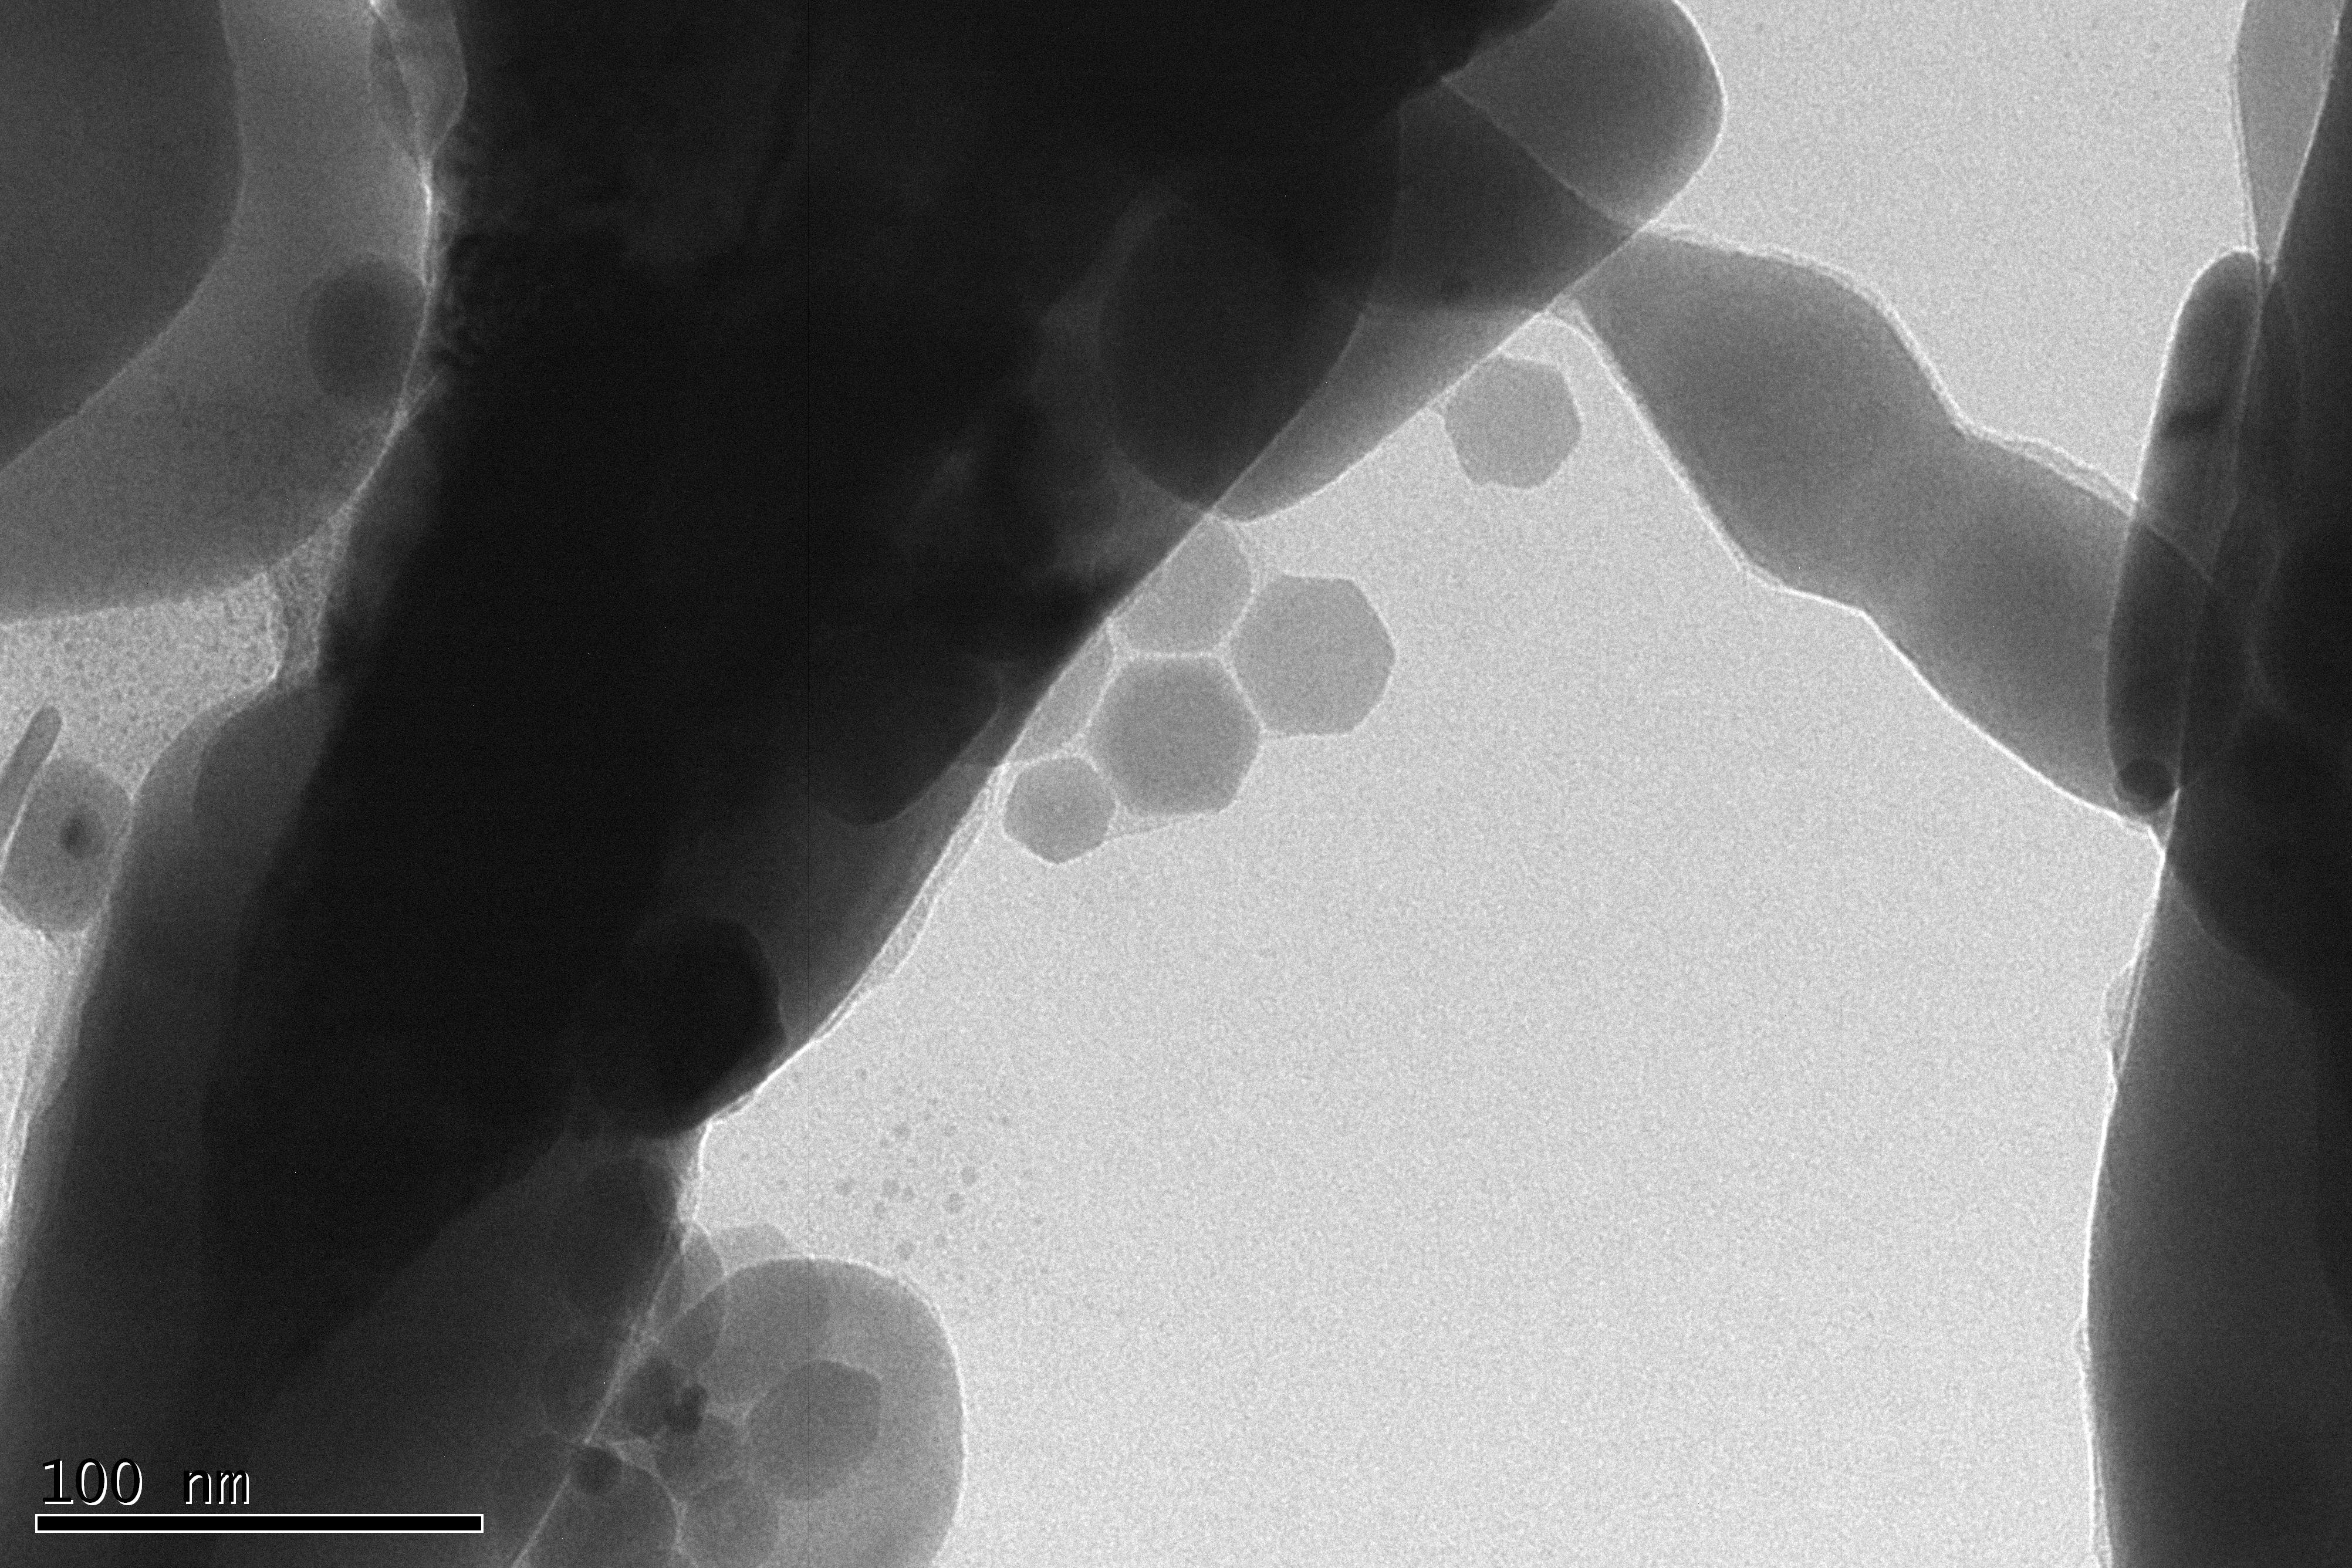
\includegraphics[width=0.33\linewidth]{Bilder/CuAu-10-1_3}}
		\caption{TEM-Aufnahmen der Probe mit einem Mengenverhältnis von 1:10 Au:\ch{Cu[DDTC]2}.}
		\label{fig:TEM-CuAu-10-1}
	\end{figure}
	
	Von den Mengenverhältnis 1:2 und 1:10 Au:\ch{Cu[DDTC]2} wurde zudem eine XRD-Messung vorgenommen, das in \cref{fig:XRD} gezeigt ist.
	Die 1:10-Probe zeigte einige scharfe Peaks zwischen 10° und 25°, die allerdings weder dem CuS, noch den Edukten zugeordnet werden können.
	Es konnte auch sonst keine Struktur gefunden werden, die hierfür in Frage kommt, die aus Kupfer und Schwefel besteht.
	Das XRD beim  Mengenverhältnis von 1:2 Au:\ch{Cu[DDTC]2} zeigt ein deutlich anderes Diffraktogramm, mit einem breiten Reflex bei etwa 41° und zwei kleinere bei 46° und 48°. Auch diese passen zu keinem der Produkte oder Edukte.
	Es liegt der Verdacht nah, dass die Proben nicht kristallin genug waren um Signale im XRD zu erzeugen.
	
	\begin{figure}[H]
		\centering
		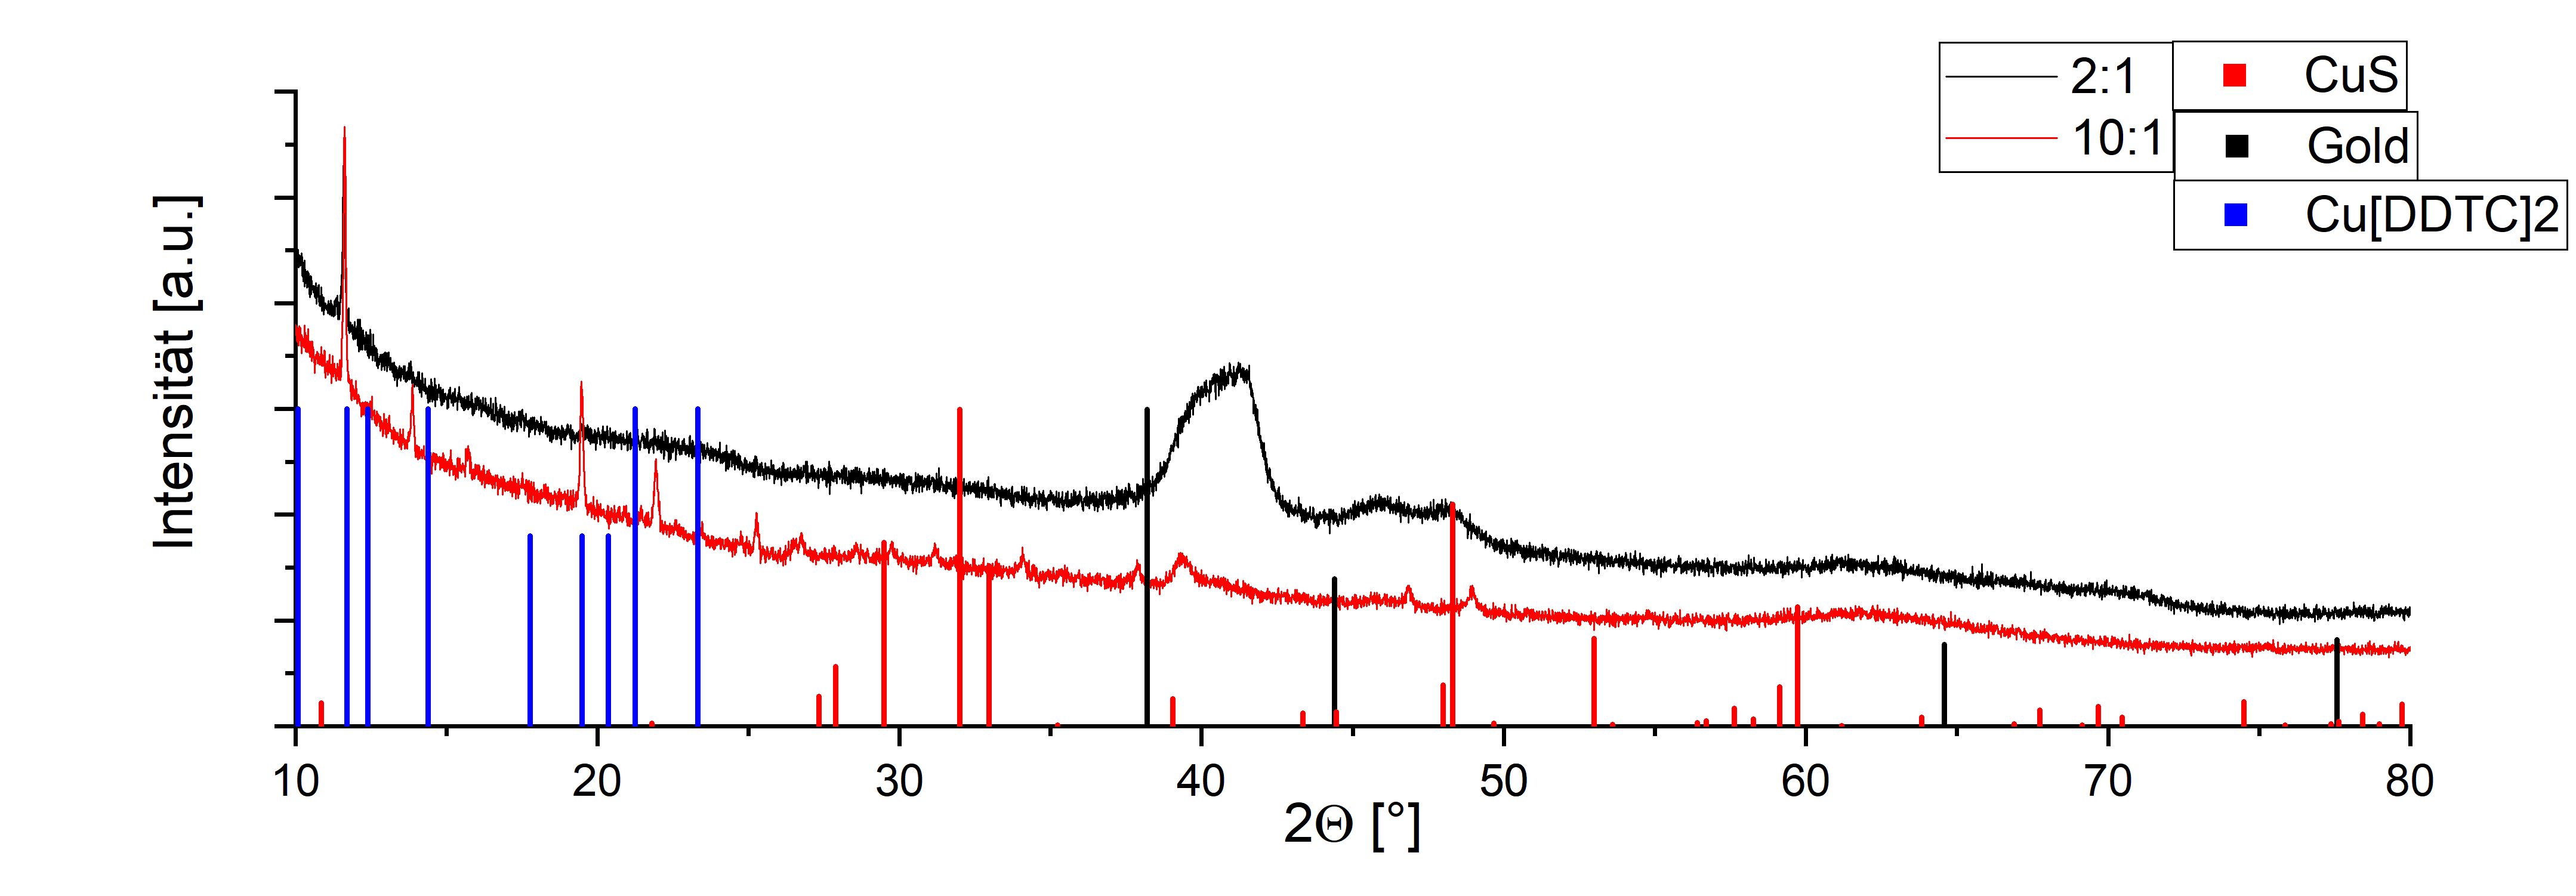
\includegraphics[width=\textwidth]{Bilder/XRD-CuS} 	
		\caption{XRD-Messung von Proben mit Mengenverhältnissen 1:2 und 1:10 Au:\ch{Cu[DDTC]2}.}
		\label{fig:XRD}
	\end{figure}
	
	
	
	

\subsection{Synthese der Gele}
	
	Nachdem die Synthese aus dem Single-Source-Precursor zusammen mit Gold-Nanopartikeln untersucht wurde, war das nächste Ziel gleiches mit Metallnanopartikelgelen durchzuführen.
	Aus diesem Grund wurden Gele mit drei verschiedenen Methoden hergestellt und untersucht.
	
	\subsubsection{Untersuchung von Hydrogelen durch Yttrium und Ytterbium}
	
		Bei fast allen Versuchen konnte nach einiger Zeit ein dunkler Niederschlag erkannt werden und die Lösung entfärbte sich bei fast allen Proben.
		Wie in \cref{fig:0625Au-Gele} zu erkennen ist, sind bei niedrigen Gold-NP-Konzentrationen von \SI{0,625}{\gram\per\liter} sowohl Yttriumchlorid als auch Ytterbiumchlorid in allen verwendeten Konzentrationen in der Lage die in kolloidaler Lösung vorhandenen Goldnanopartikel auszufällen.
		Bei höheren Goldkonzentrationen konnte ein deutlicher Unterschied zwischen Ytterbium und Yttrium festgestellt werden. 
		Währenddessen die Yttriumlösungen auch die höheren Gold-NP-Konzentrationen von \num{1,25} und \SI{2,5}{\gram\per\liter} komplett ausfällen konnte, war dies mit Ytterbium in gleicher Konzentration nicht möglich, wie in \cref{fig:1Y-Yb-Gele} durch die immer noch vorhandene Rotfärbung zu erkennen ist.
		
		\begin{figure}[H]
			\centering
			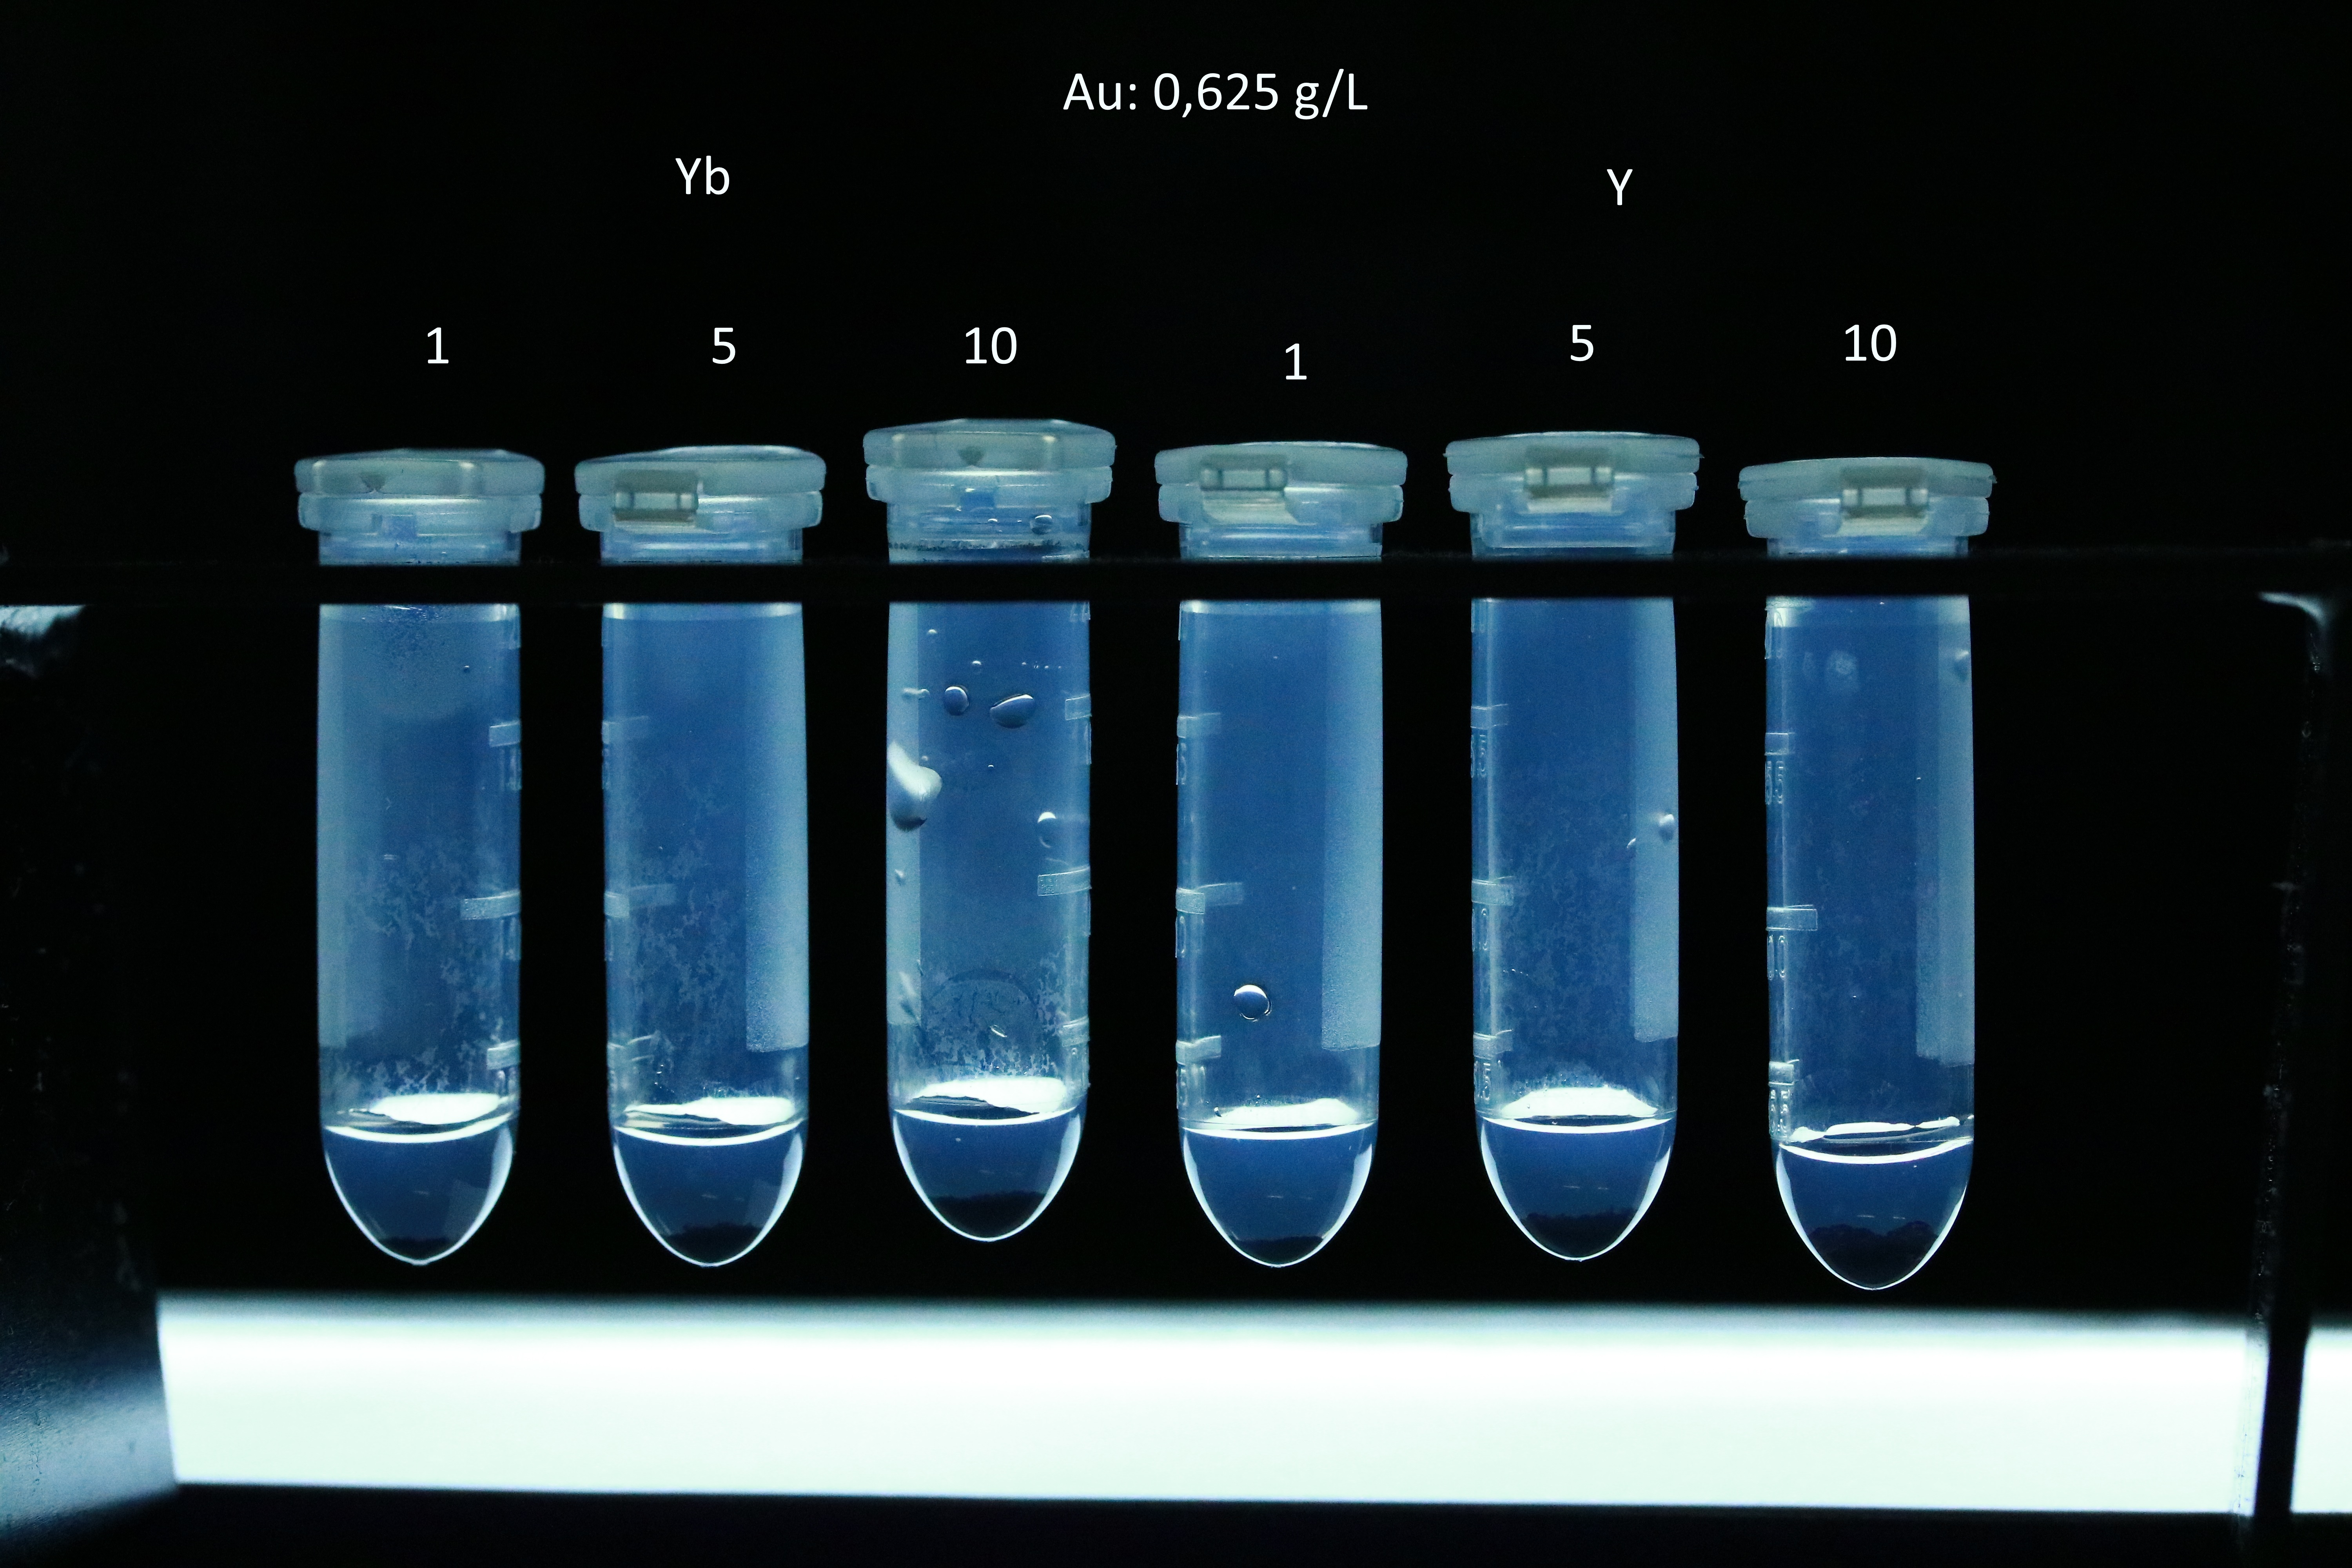
\includegraphics[width=0.6\textwidth]{Bilder/0625Au-Gele} 	
			\caption{Übersicht der Gele mit 0,625 g/L Goldlösung und Salzlösungen mit 1;5;10 mM Yb$^{3+}$ und Y$^{3+}$.}
			\label{fig:0625Au-Gele}
		\end{figure}
	
		\begin{figure}[H]
			\centering
			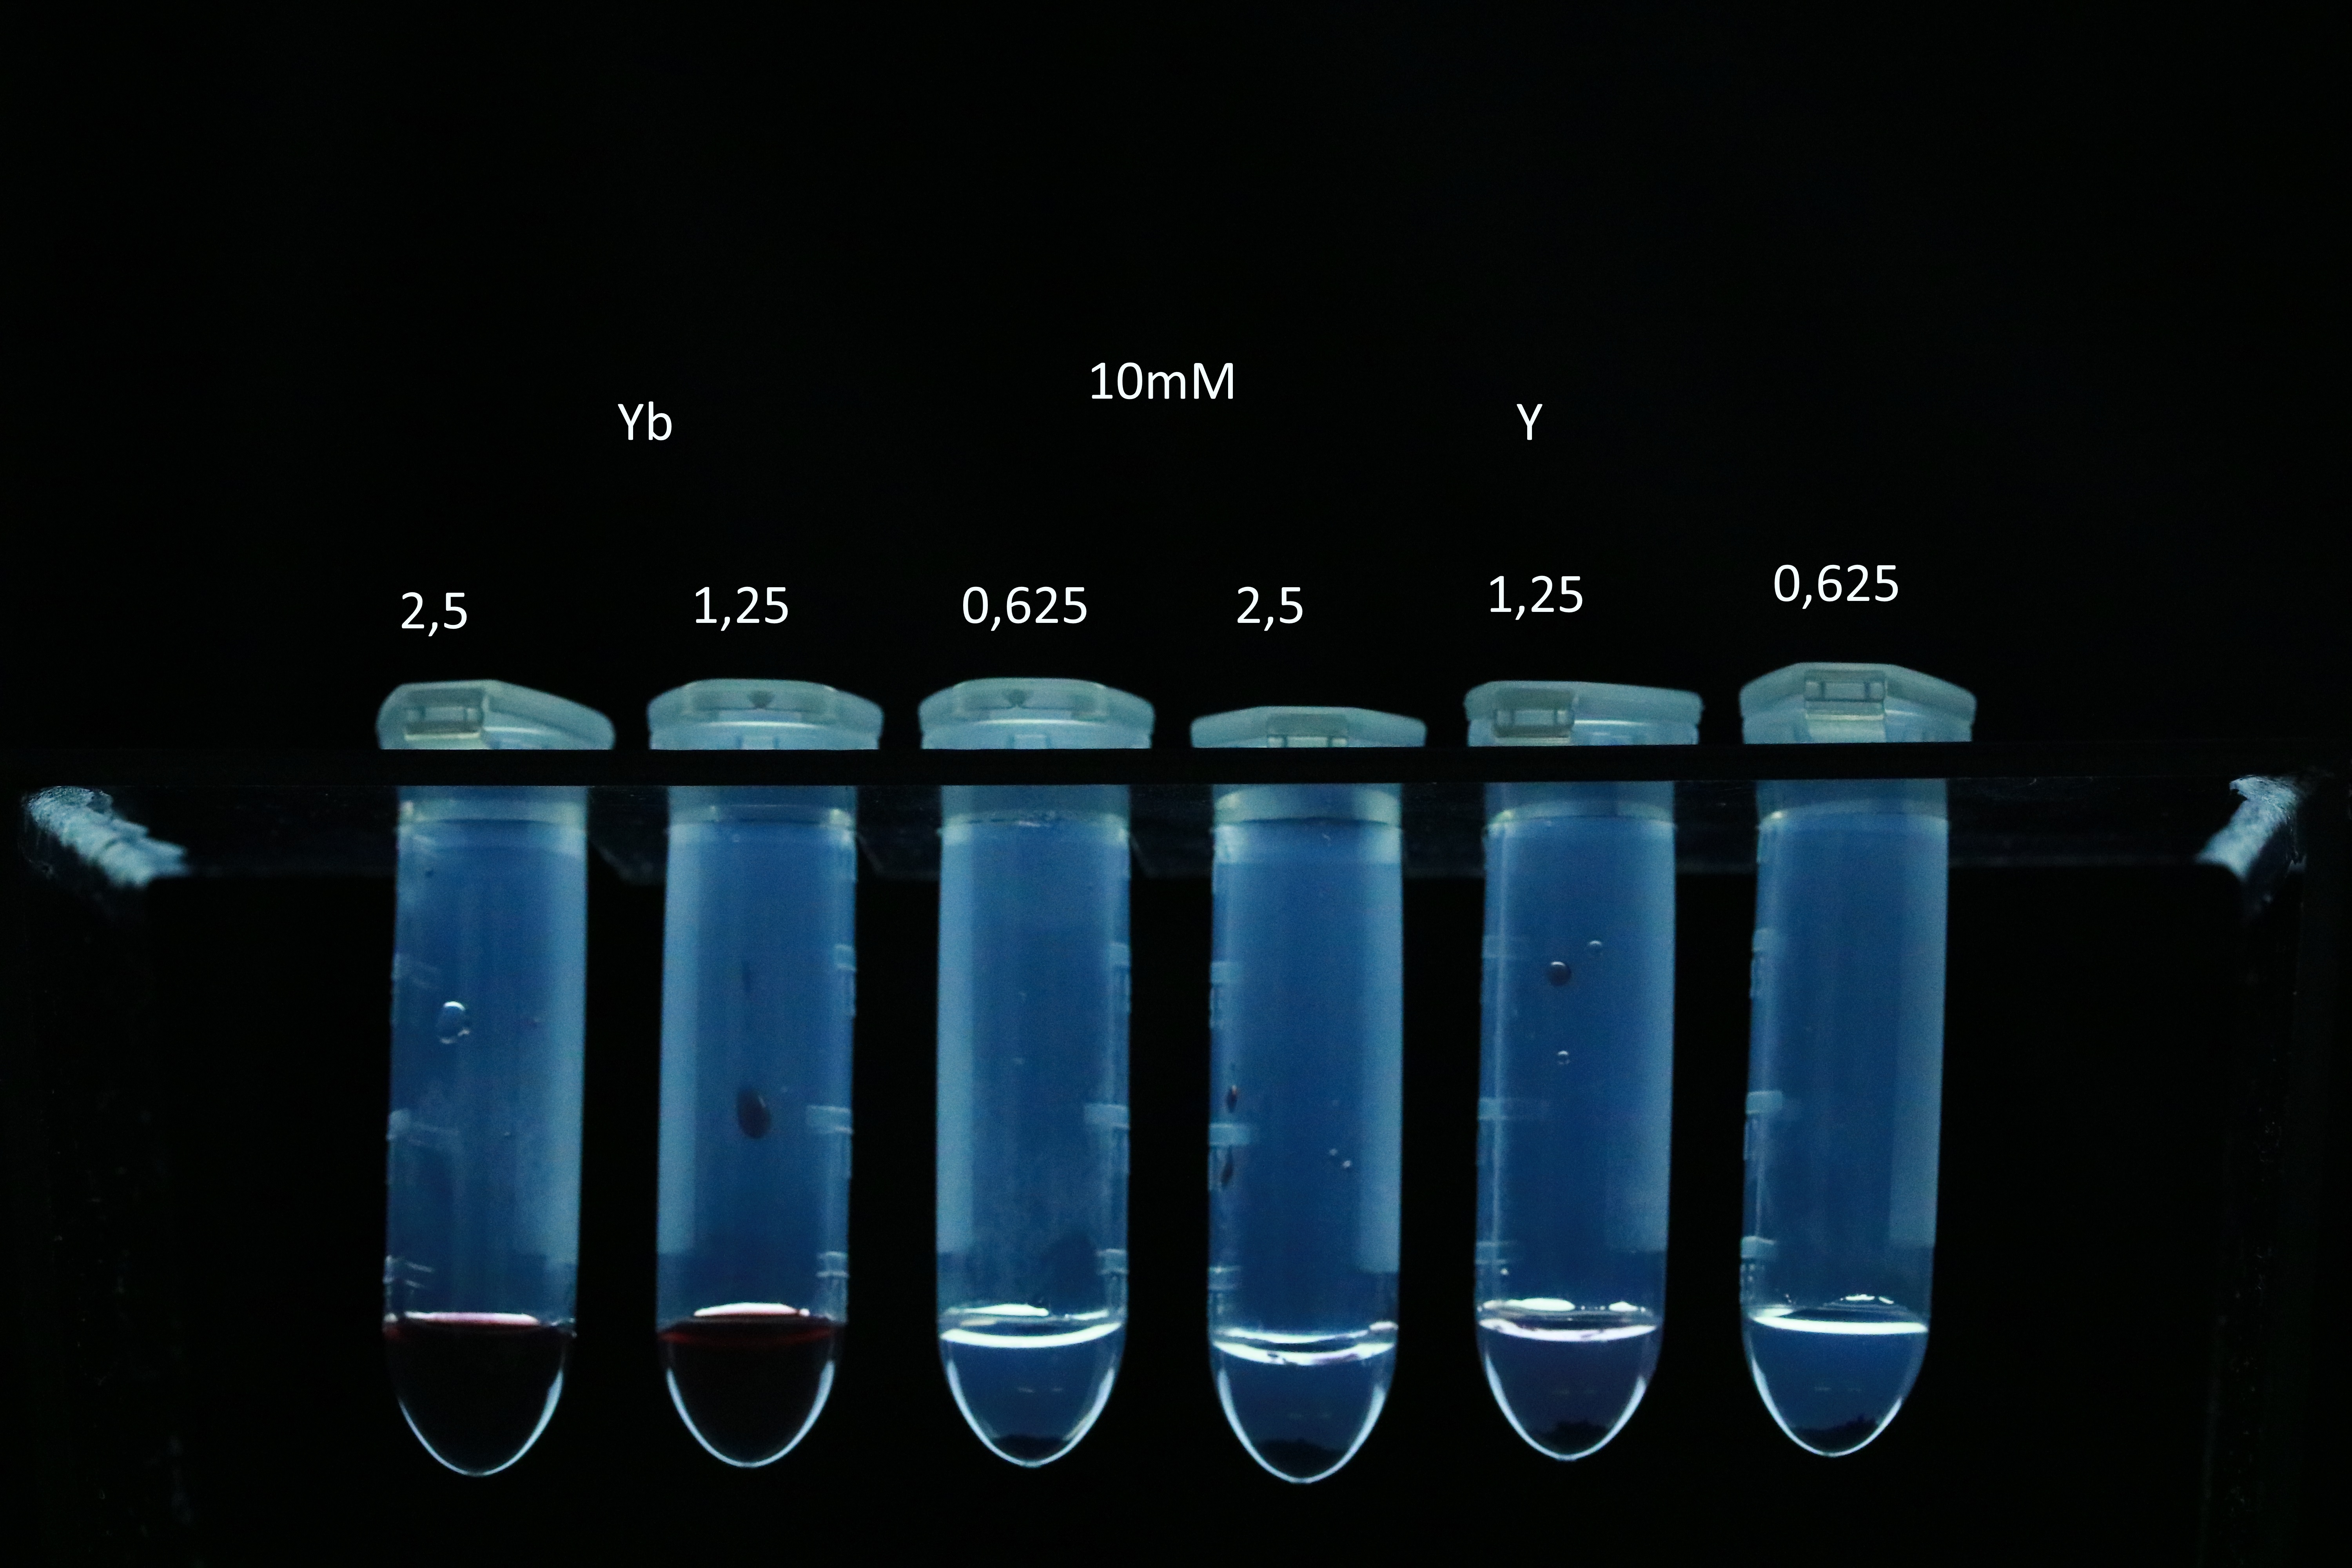
\includegraphics[width=0.6\textwidth]{Bilder/1Y-Yb-Gele} 	
			\caption{Übersicht der Gele mit 10 mM Yb$^{3+}$ und Y$^{3+}$-Lösung und 2,5; 1,25; 0,625 g/L Gold-NP-Lösung.}
			\label{fig:1Y-Yb-Gele}
		\end{figure}
		
		Da es bei den Proben mit Yttrium immer zu einer vollständigen Entfärbung kam, also sämtliches Gold aus der Lösung abgelagert wurde, wurde sich bei weiteren Untersuchungen auf diese beschränkt.
		Um festzustellen, ob es sich bei dem gebildeten Niederschlag um Gele handelte wurden TEM-Aufnahmen von einigen Proben vorgenommen.
		Dabei wurden jeweils die Extreme der verwendeten Konzentrationen näher untersucht.
		
		\begin{figure}[H]
			\centering
			\subfloat[\label{fig:Au-Y-}]{%
				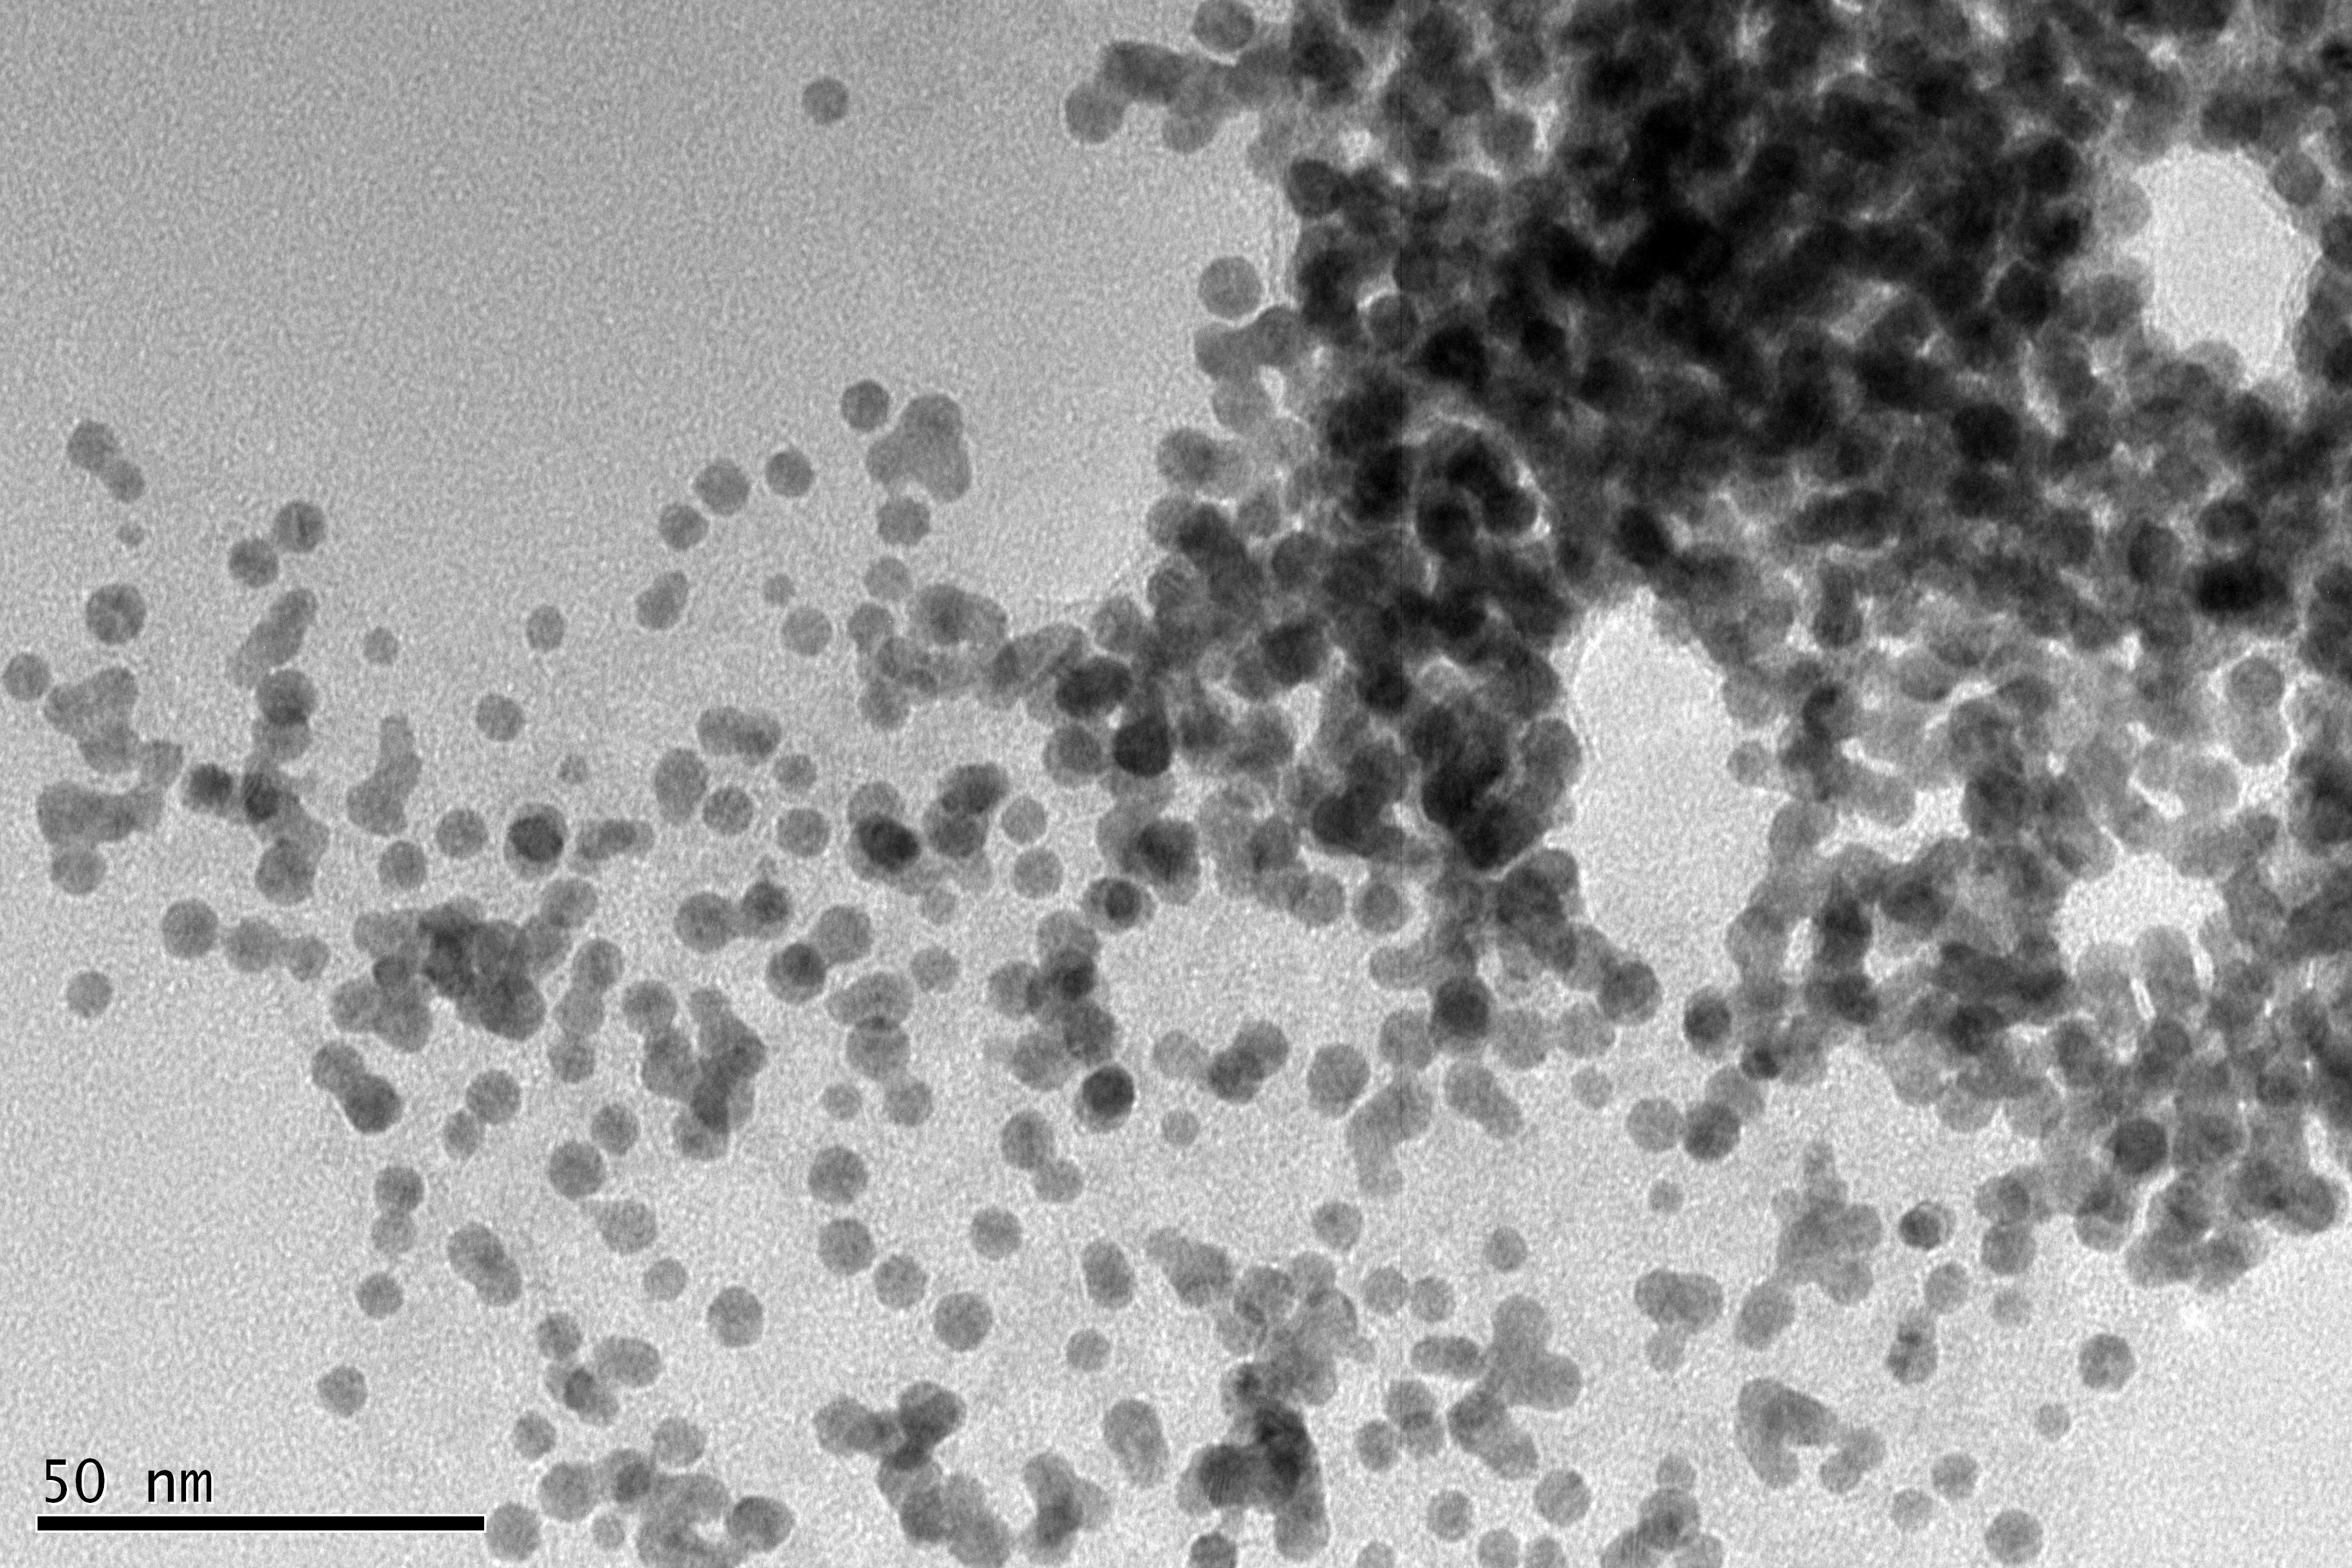
\includegraphics[width=0.45\linewidth]{Bilder/Au-Y-}}
			\subfloat[\label{fig:Au+Y-}]{%
				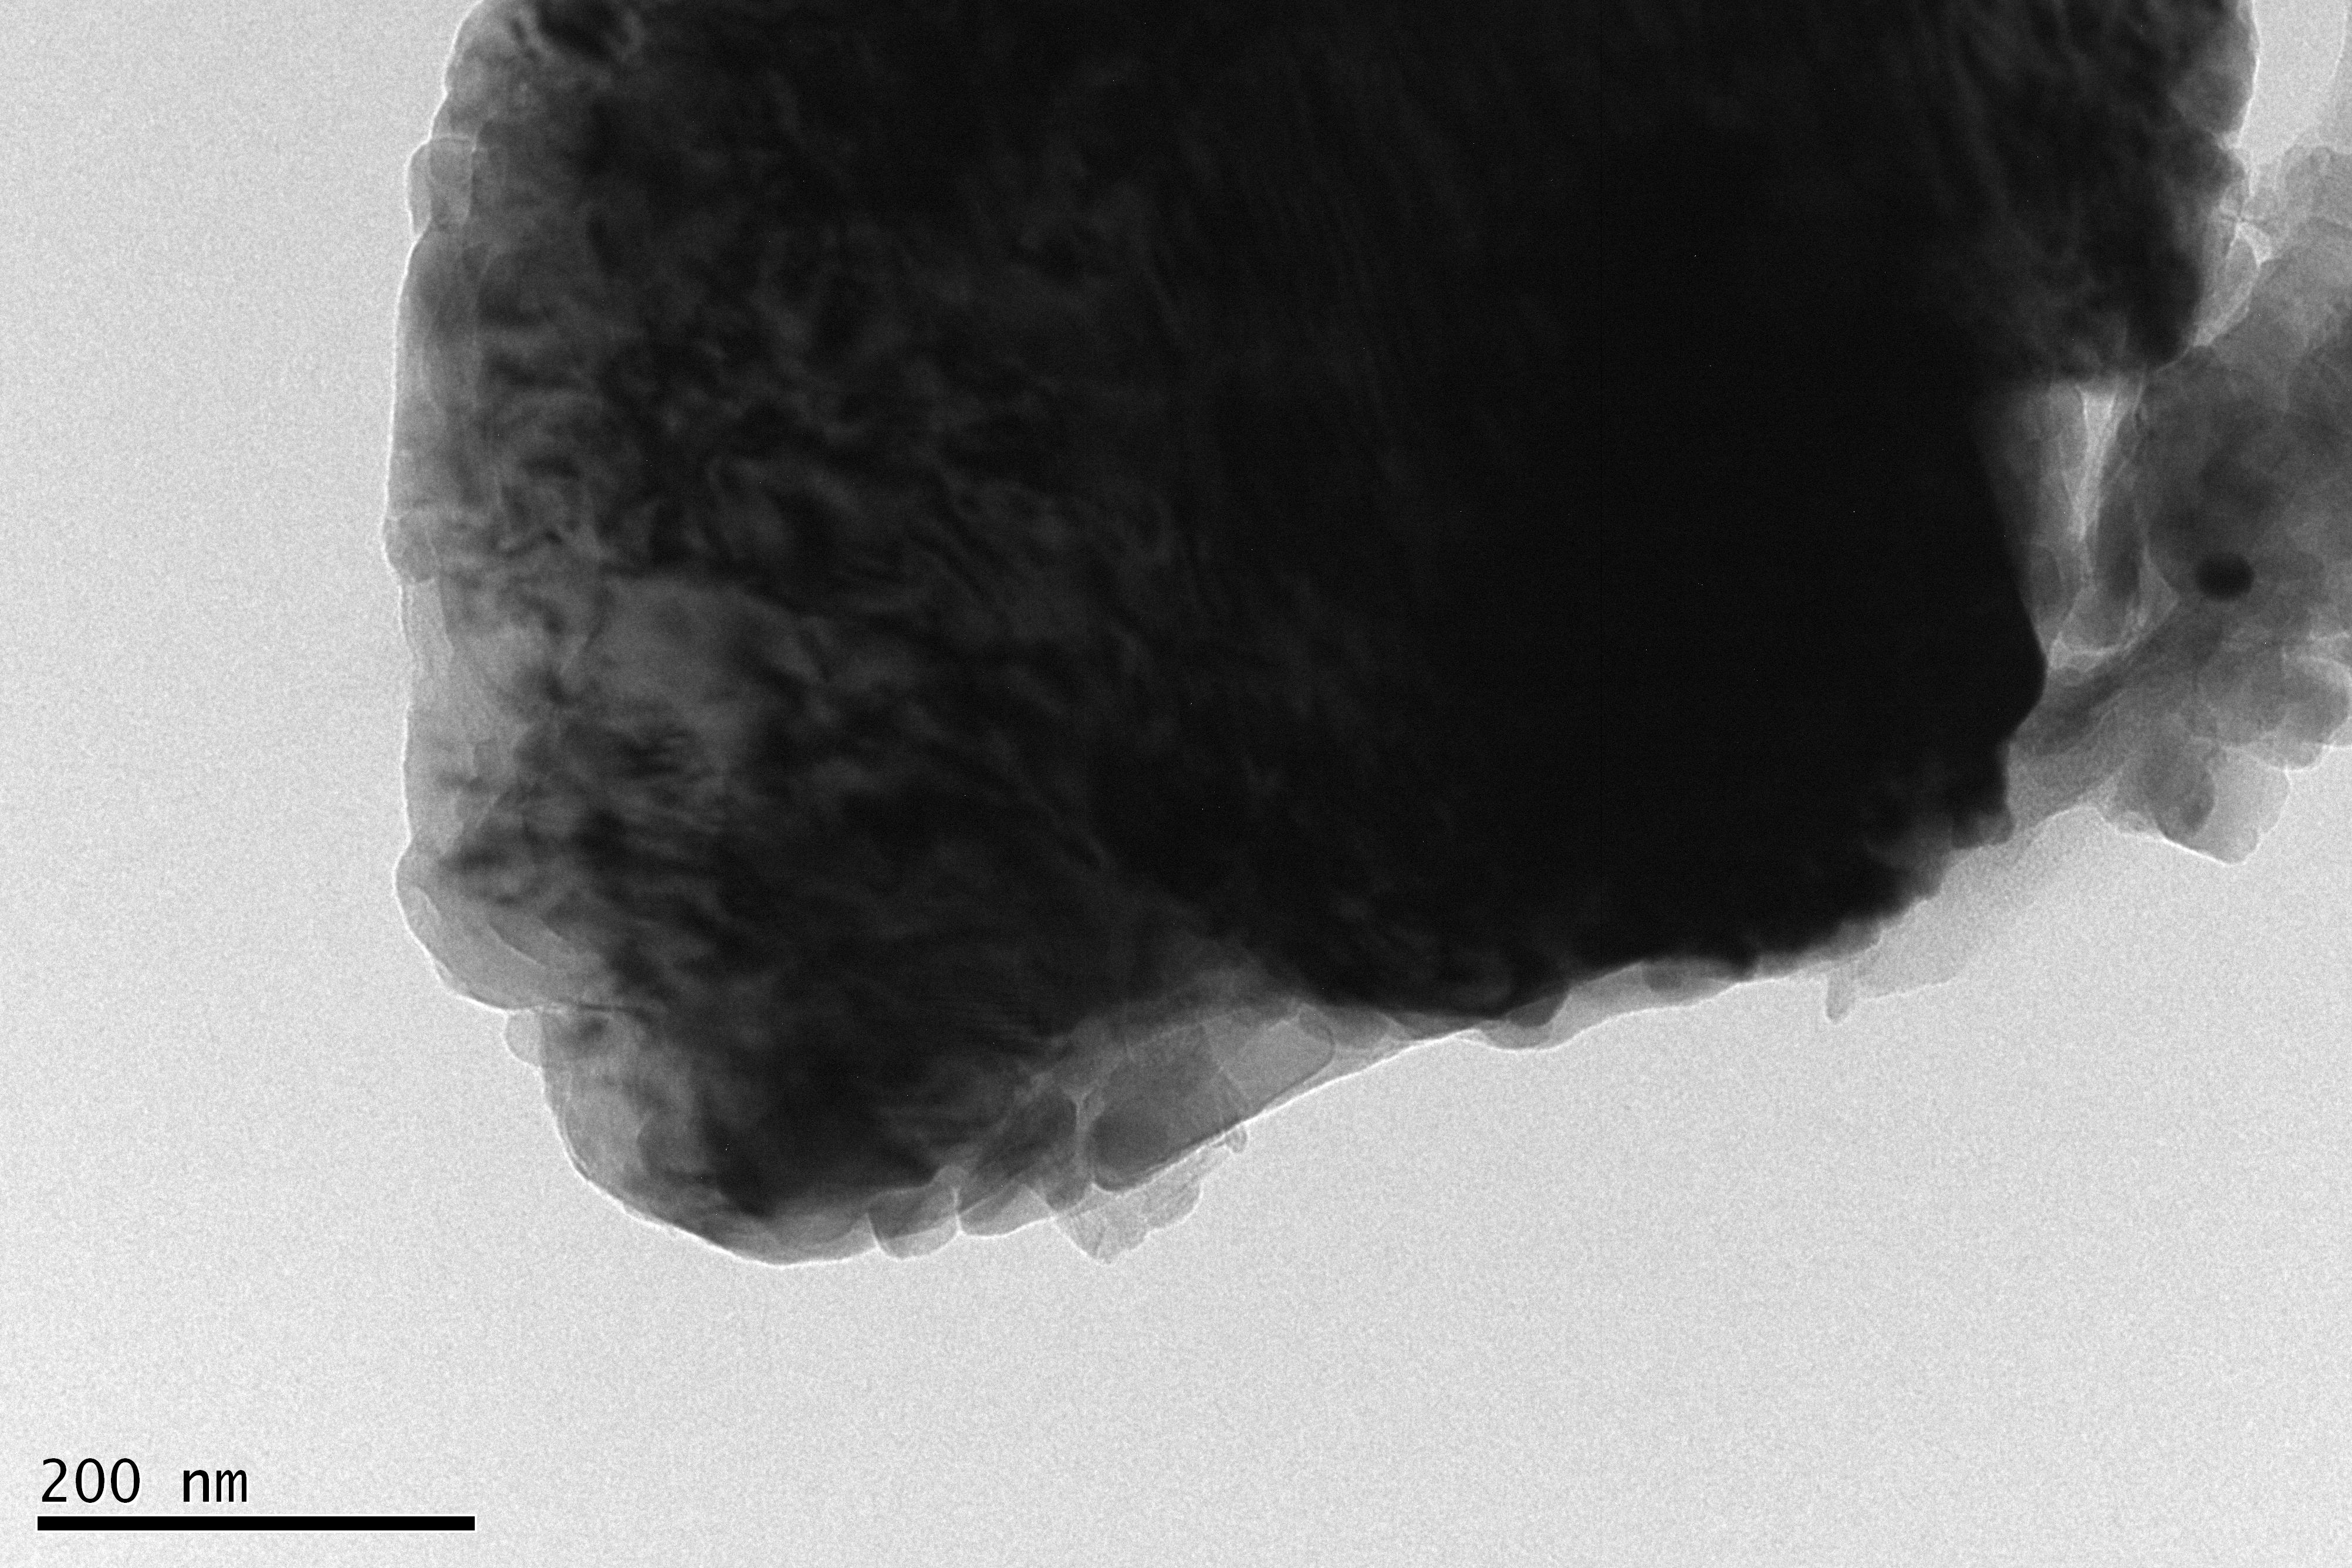
\includegraphics[width=0.45\linewidth]{Bilder/Au+Y-}}\\
			\subfloat[\label{fig:Au-Y+}]{%
				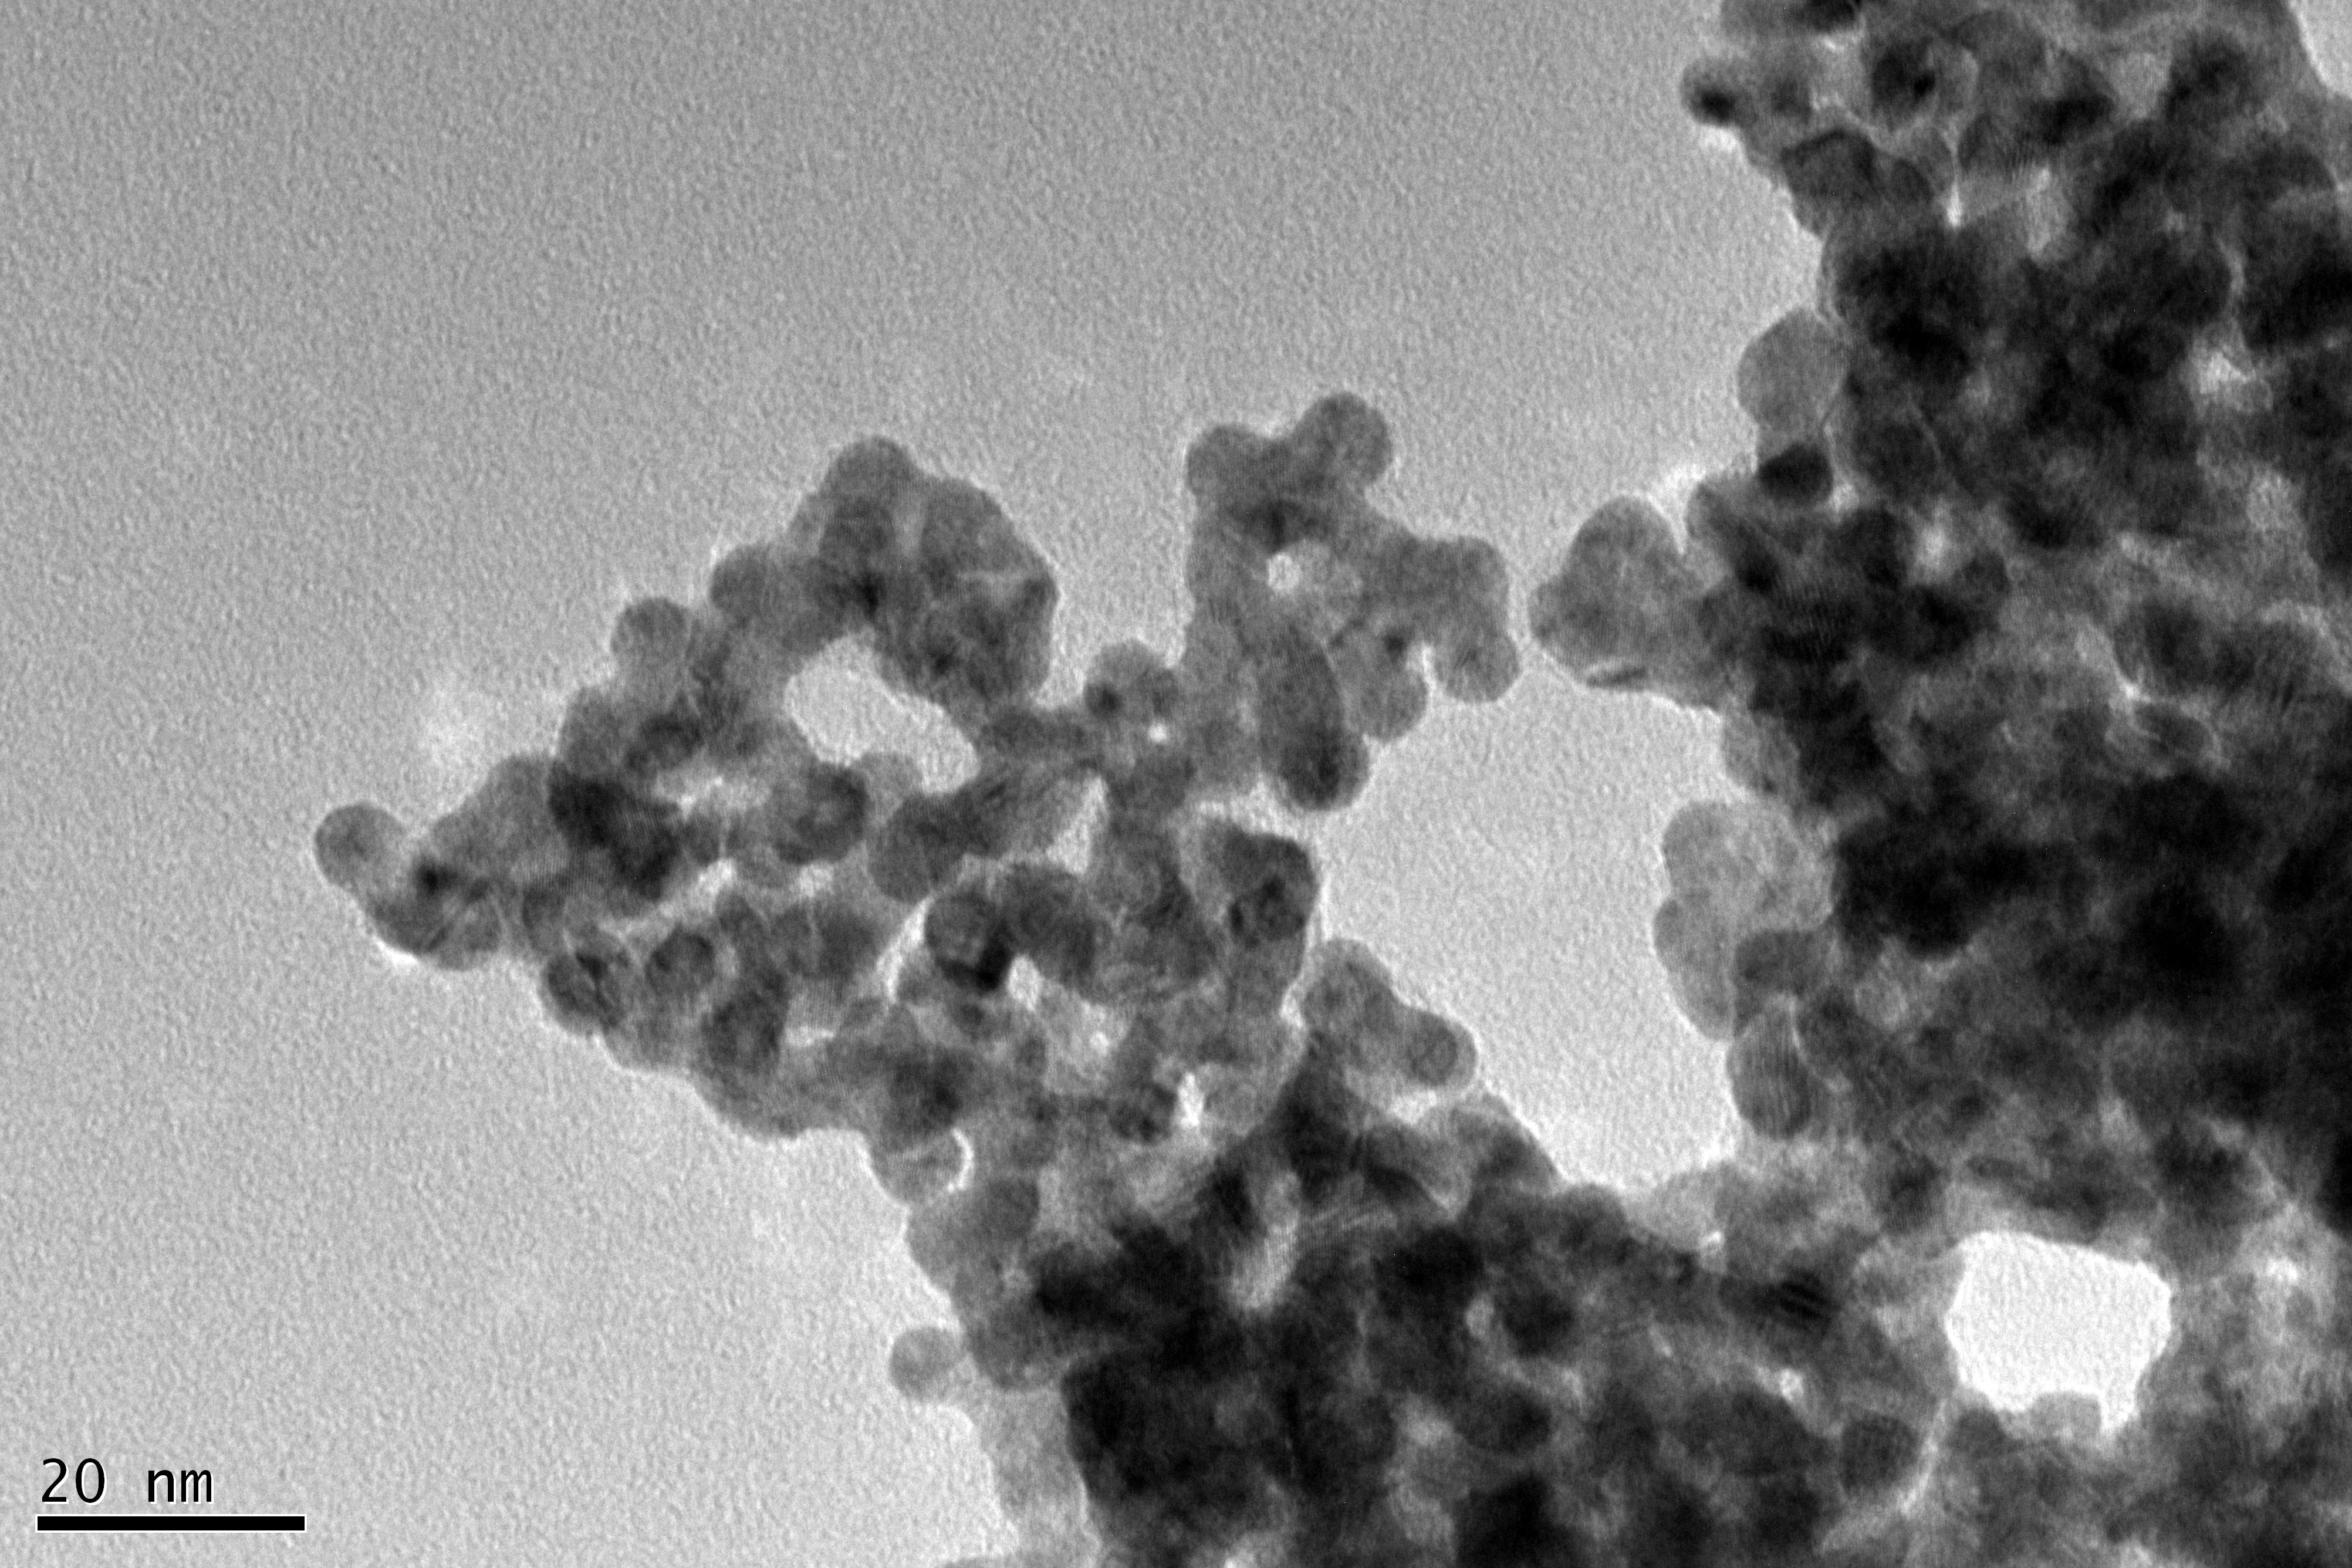
\includegraphics[width=0.45\linewidth]{Bilder/Au-Y+}}
			\subfloat[\label{fig:Au+Y+}]{%
				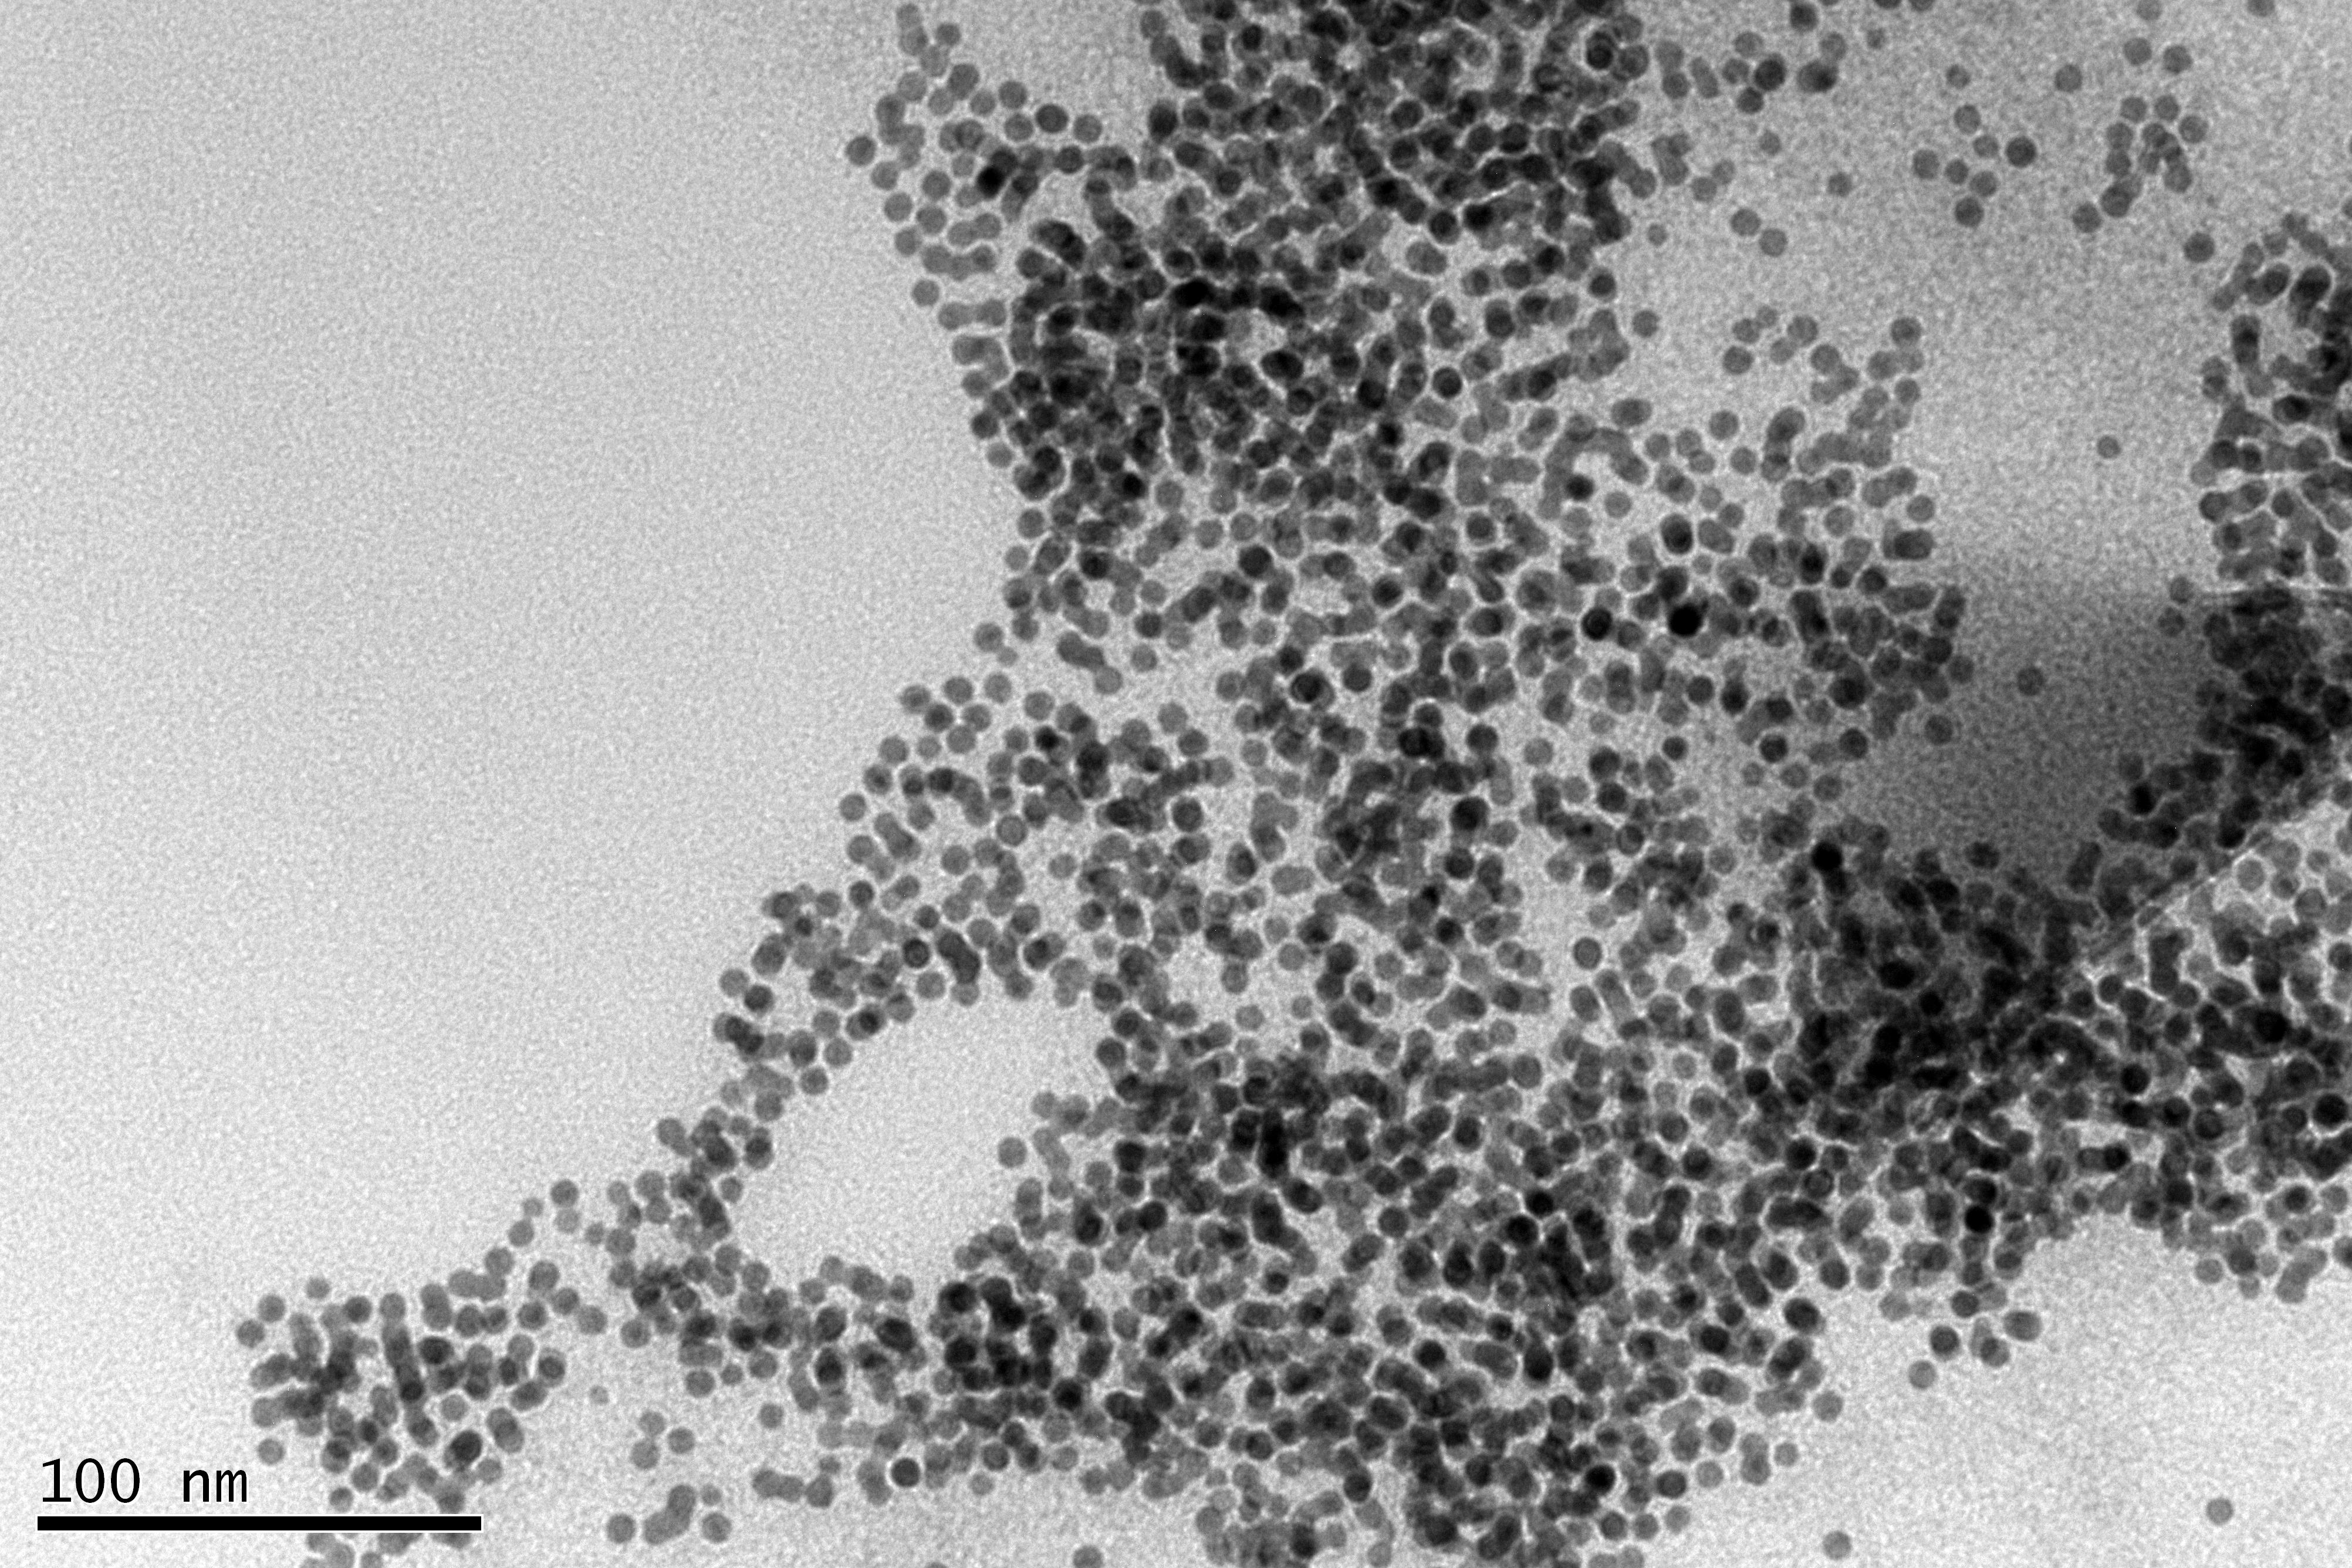
\includegraphics[width=0.45\linewidth]{Bilder/Au+Y+}}
			\caption{TEM-Bilder nach Zugabe von Yttriumchlorid mit den Konzentrationen: \emph{(a)}:~Au:~\SI{0,625}{\gram\per\liter}, Y: 1~mM;
			\emph{(b)}:~Au:~\SI{2,5}{\gram\per\liter}, Y: 1~mM
			\emph{(c)}:~Au:~\SI{0,625}{\gram\per\liter}, Y: 10~mM
			\emph{(d)}:~Au:~\SI{2,5}{\gram\per\liter}, Y: 10~mM} 
			\label{fig:Y-Gele}
		\end{figure}
		
		Die TEM-Bilder zeigten, dass es zu deutlichen Unterschieden bei den verschiedenen Konzentrationen kommt.
		So entstanden bei hoher Goldkonzentration und niedriger Yttriumkonzentration keine Gele sondern nur ein großer Klumpen (\cref{fig:Au+Y-}).
		Bei hoher Goldkonzentration und hoher Yttriumkonzentration hingegen lagen die Partikel alle seperat voneinander vor und es wurde also auch hier kein Gel gebildet(\cref{fig:Au+Y+}). 
		Bei den Versuchen mit den geringen Goldkonzentrationen konnte bei beiden Yttriumkonzentration eine Anlagerung der Gold-NP aneinander beobachtet werden.
		Bei geringer Yttriumkonzentration lagen jedoch ein größerer Teil der Partikel einzeln vor, wie \cref{fig:Au-Y-} zeigt. 
		Das, was dem Aussehen klassischer Nanopartikelgele am nächsten kam, war die Probe mit niedriger Goldkonzentration und höherer Yttriumkonzentration (\cref{fig:Au-Y+}). 
		Hier waren die Partikel miteinander venetzt und bildeten dabei Hohlräume aus.
		
		
	\subsubsection{Untersuchung von citratstabilisierten Gelen}
		
		Die für die Gelierung hergestellten Silber- und Goldpartikeln wurden per UV-vis-Absorptionsspektroskopie untersucht.
		Sie zeigten typische Absorptionsmaxima bei $\lambda_{Gold}$=\SI{525}{\nano\meter} und $\lambda_{Silber}$=\SI{412}{\nano\meter}, wie \cref{fig:Abs-cit} zeigt.
		Bei dem Absorptionsspektrum der Goldnanopartikel ist außerdem eine kleine Schulter bei \SI{620}{\nano\meter} zu erkennen, was darauf hindeutet, dass nicht alle Partikel monodisperse sphärische Partikel sind.  
		\begin{figure}[H]
			\centering
			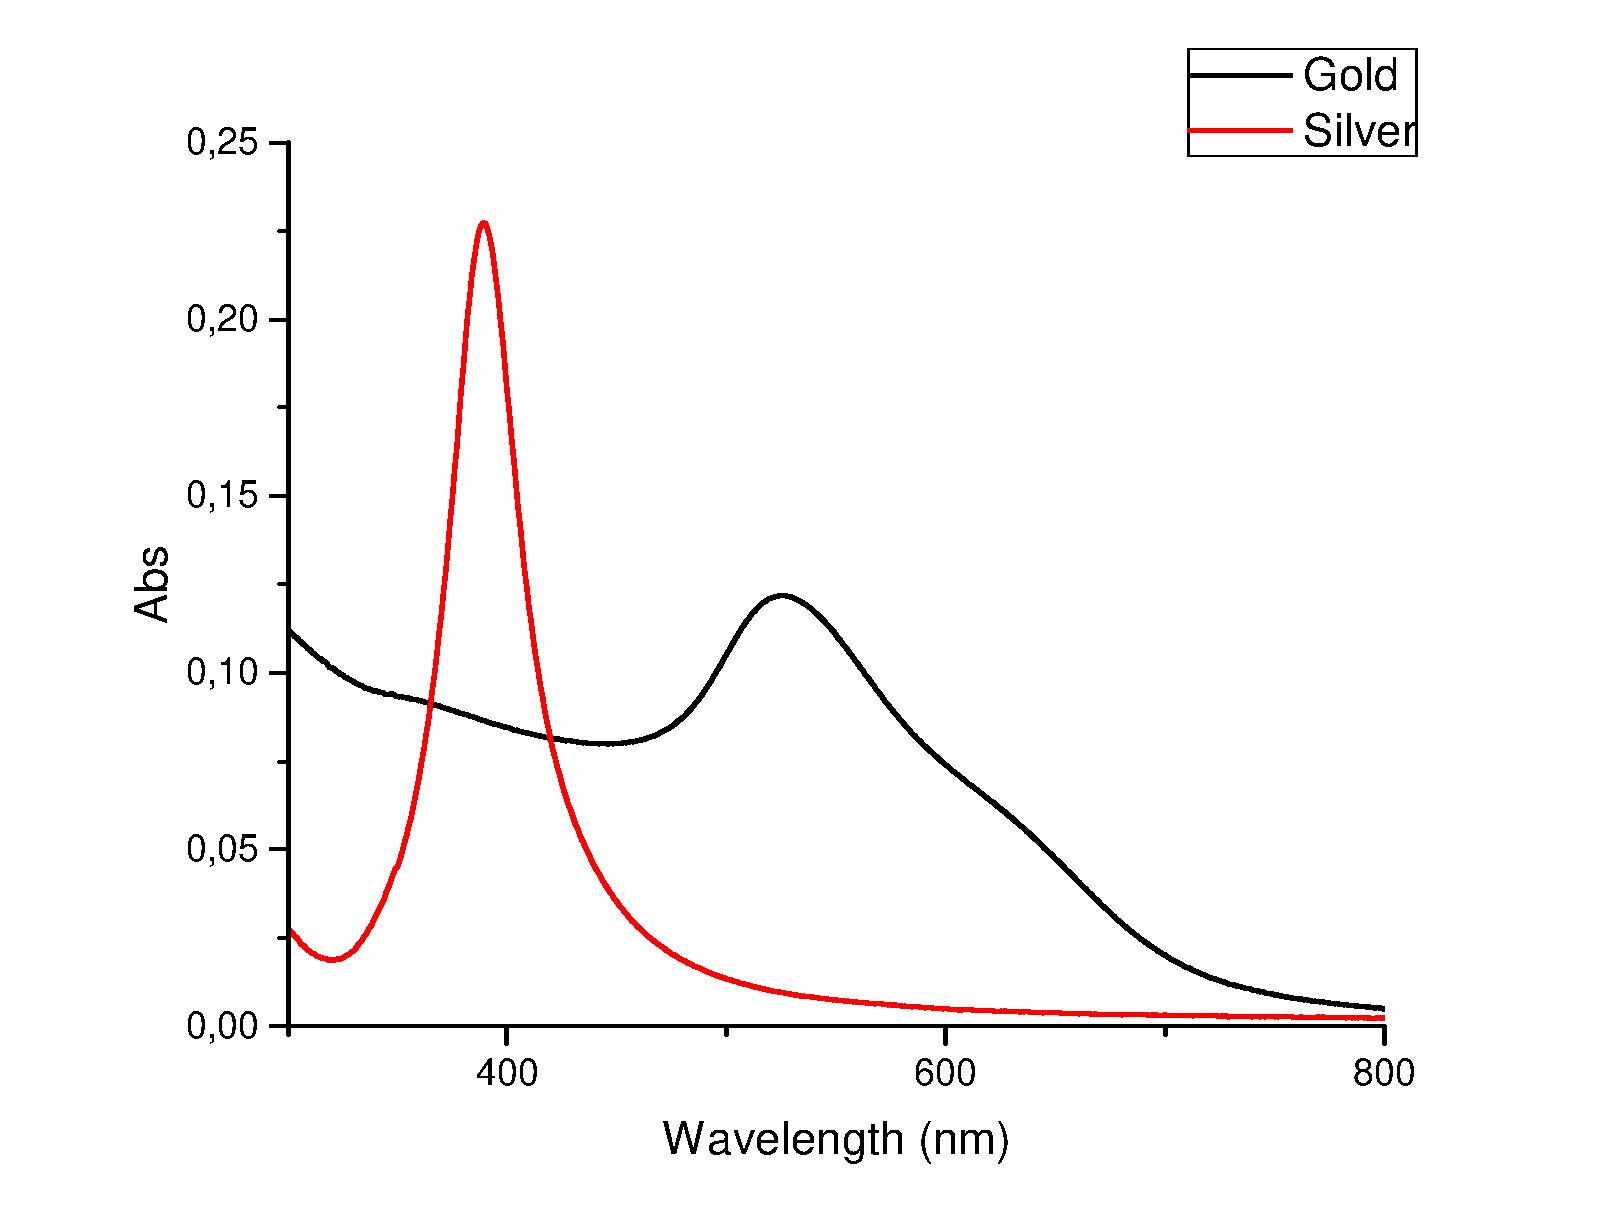
\includegraphics[width=0.6\textwidth]{Bilder/Citrat-NP} 	
			\caption{UV-vis-Absorptionsspektren von Gold-NP und Silber-NP.}
			\label{fig:Abs-cit}
		\end{figure}
	
		Da bei den Versuchen mit reinem Gold und Silber keine festen Gele entstanden sind wurden diese auch nicht weiter untersucht.
		Im Vergleich zu den Hydrogelen, ist das Gel während des Austausches der flüssigen Phase zu TOP zu etwa ein Drittel des Ausgangsvolumen zusammengeschrumpft.
		Von den bimetallischen Gelen aus Gold- und Silbernanopartikeln wurden TEM-Bilder nach dem Phasentransfer in TOP aufgenommen.
		Es ist ein Netzwerk zu erkennen, das aus kleinen Partikeln ($\approx$~\SI{10}{\nano\meter}), die miteinander Verknüpft sind und dabei viele große Zwischenräume ausbildet, wie \cref{fig:Gel-C} zeigt. 
		
		\begin{figure}[H]
			\centering
			\subfloat[\label{fig:Gel-C-1}]{%
				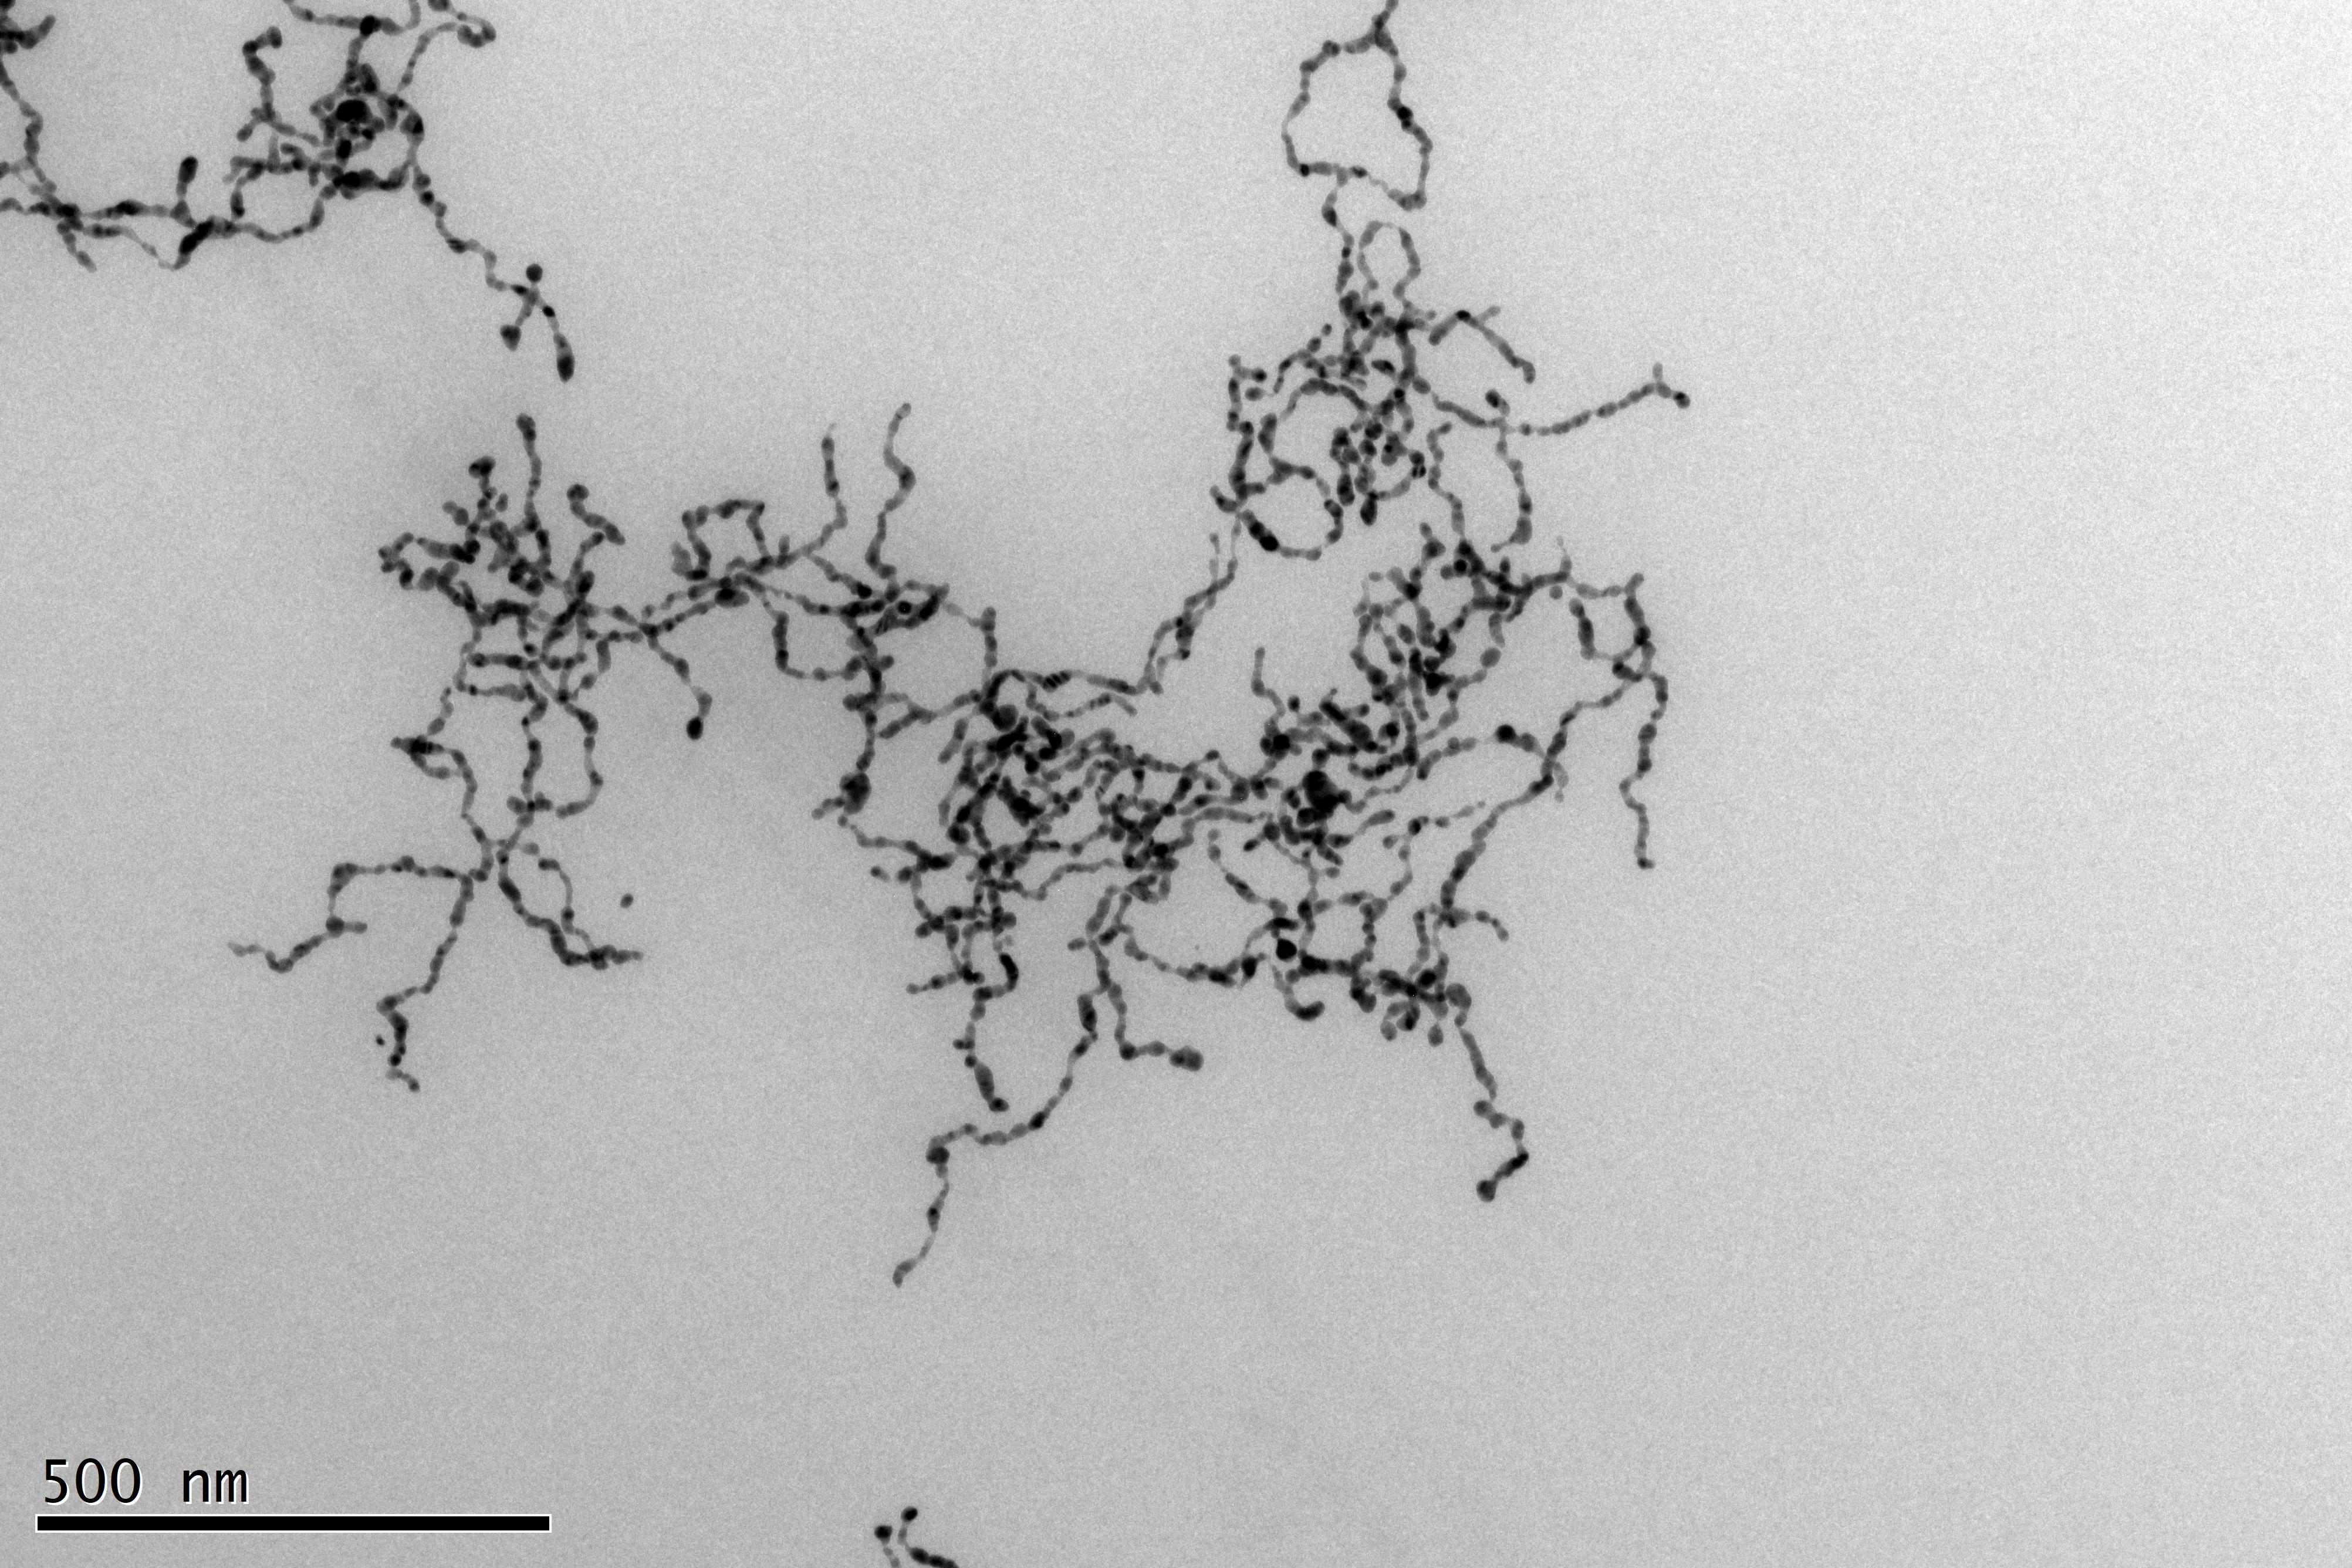
\includegraphics[width=0.33\linewidth]{Bilder/Gel-C-1}}
			\subfloat[\label{fig:Gel-C-2}]{%
				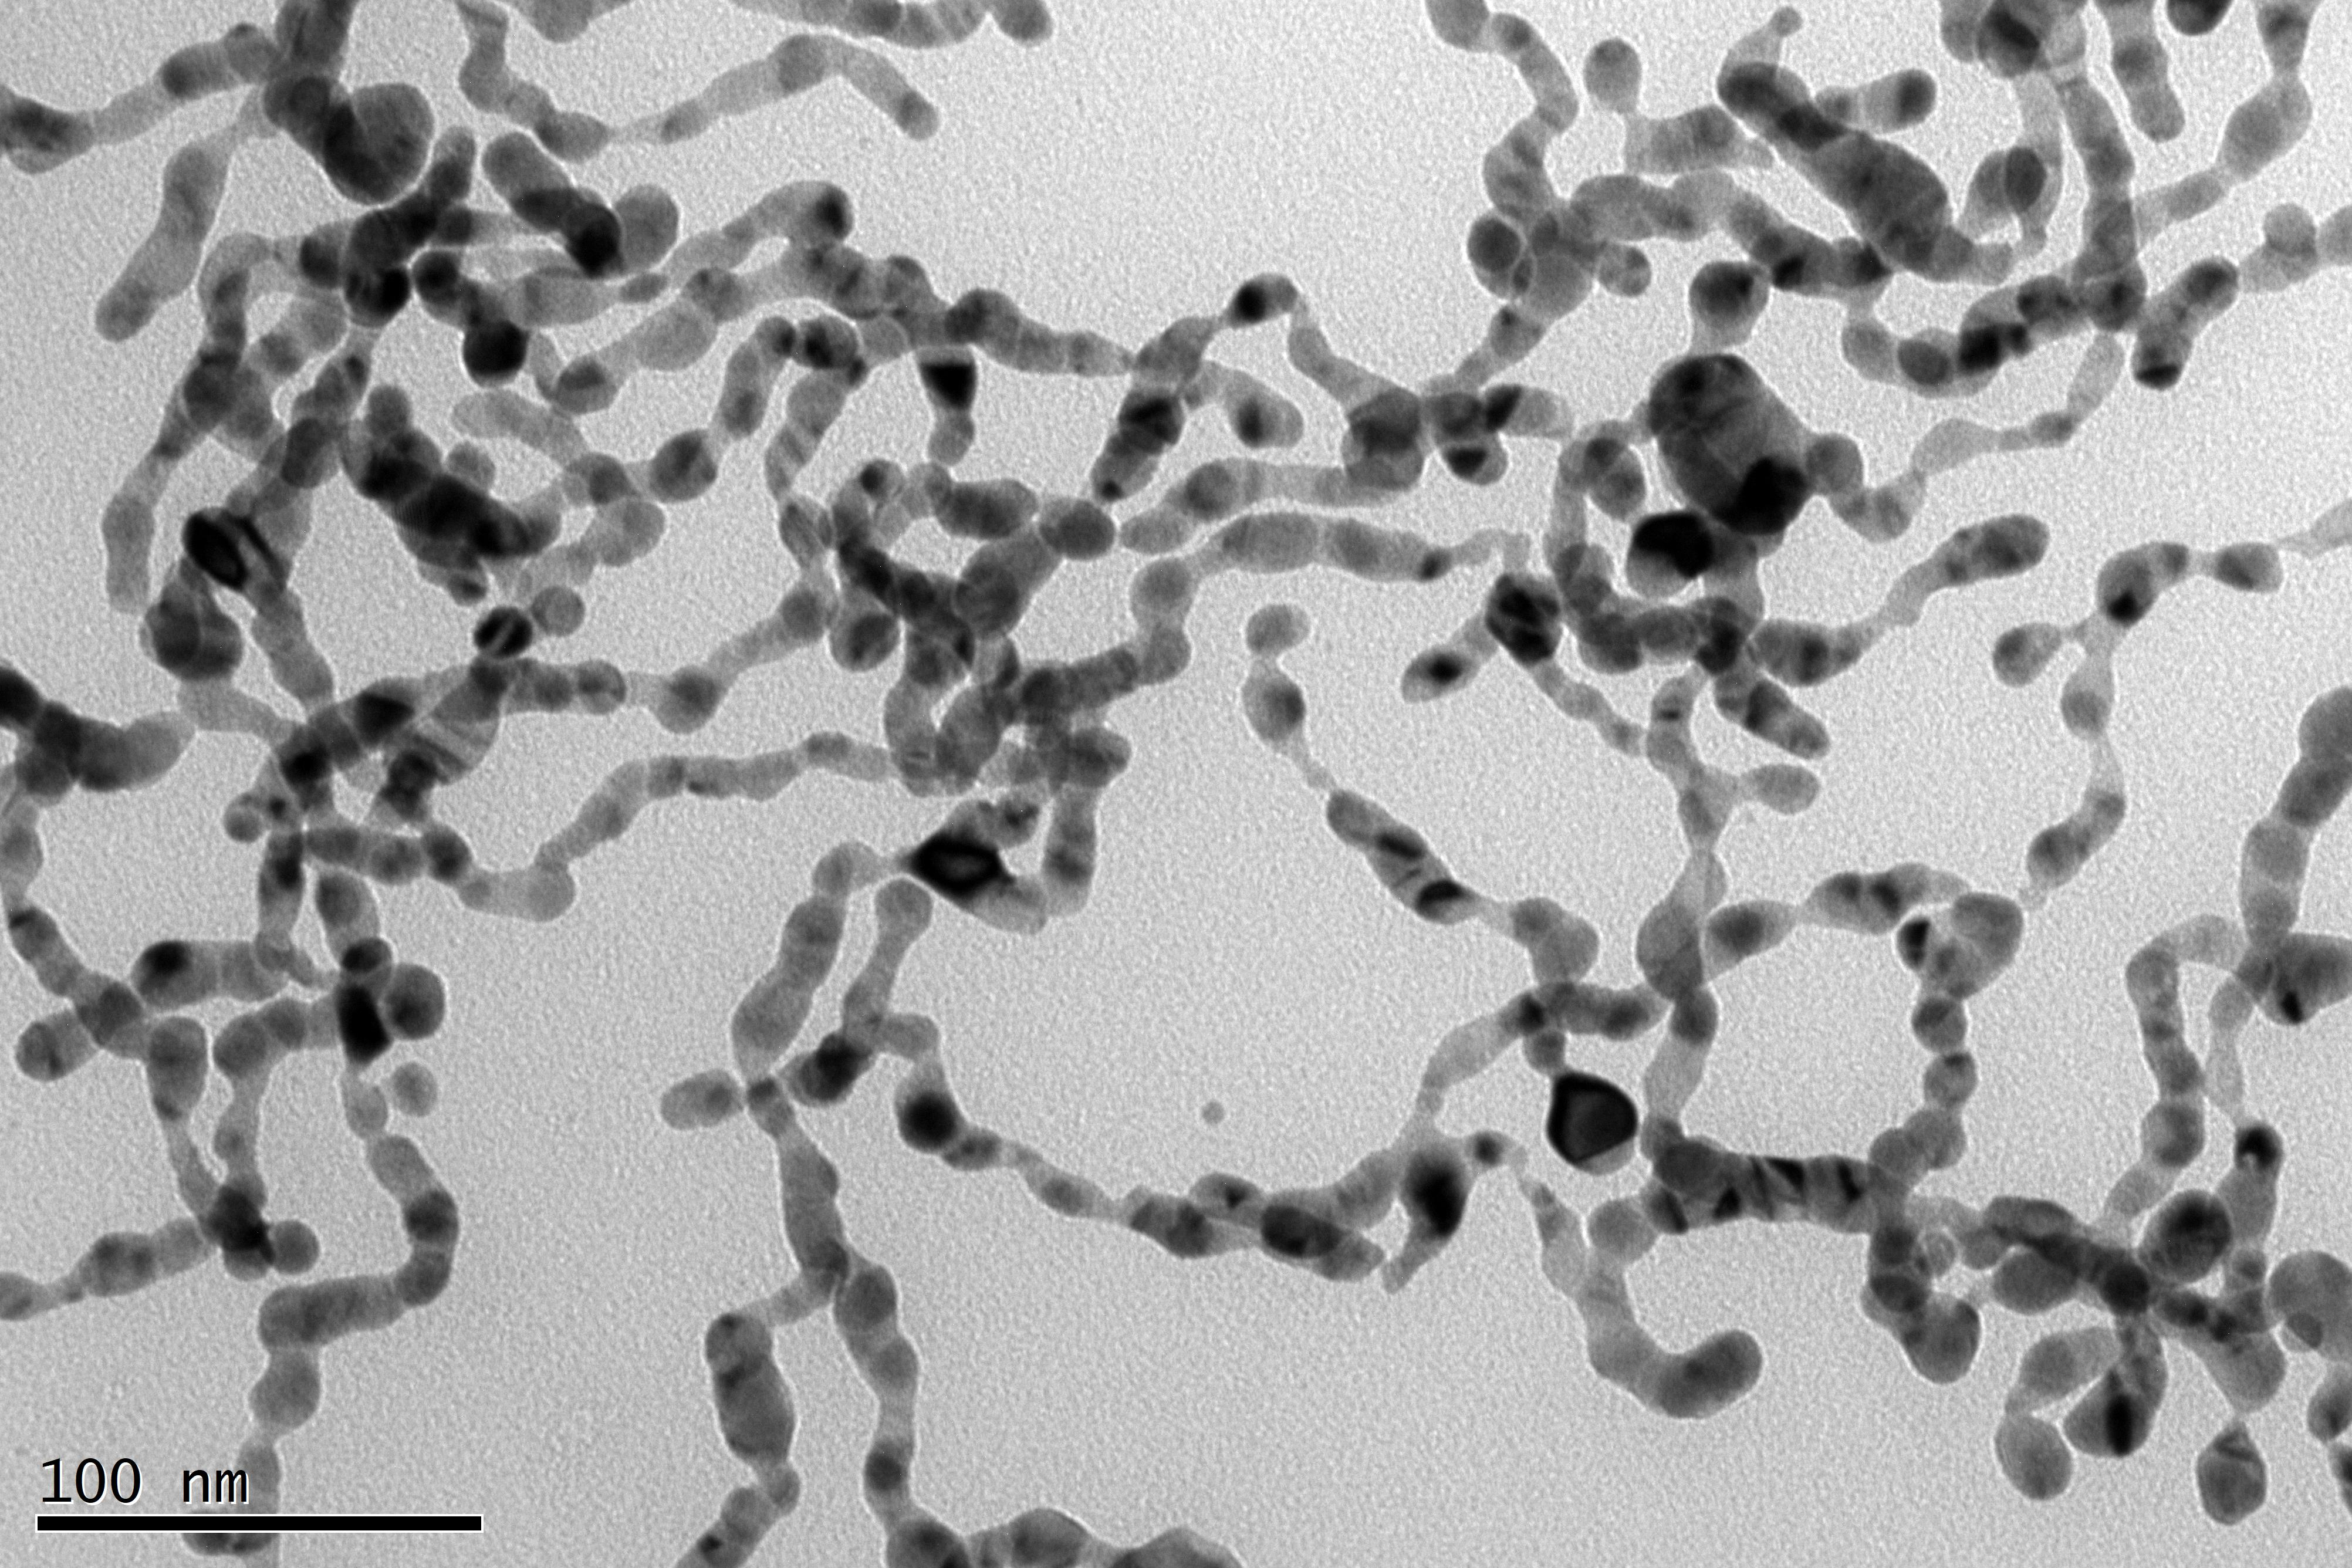
\includegraphics[width=0.33\linewidth]{Bilder/Gel-C-2}}
			\subfloat[\label{fig:Gel-C-3}]{%
				\includegraphics[width=0.33\linewidth]{Bilder/gel-C-3}}
			\caption{TEM-Bilder der citratstrabilisierten Gele in TOP.}
			\label{fig:Gel-C}
		\end{figure}
		
	\subsubsection{Untersuchung der Gele aus ethanolischem Ansatz}
		
		Da bei diesen Gelen der Schritt der Nukleation und der Schritt der Gelierung nicht separat voneinander Ablaufen, war ein groberes, weniger gleichmäßiges Gel als bei den citratstabilisierten zu erwarten.
		Dies war auch wie \cref{fig:Gel-C} zeigt der Fall.
		Insgesamt zeigt das Gel weniger Zwischenräume bei einem deutlich größeren Partikeldurchmesser ($\approx$~\SI{100}{\nano\meter}).
		
		\begin{figure}[H]
			\centering
			\subfloat[\label{fig:Gel-E-1}]{%
				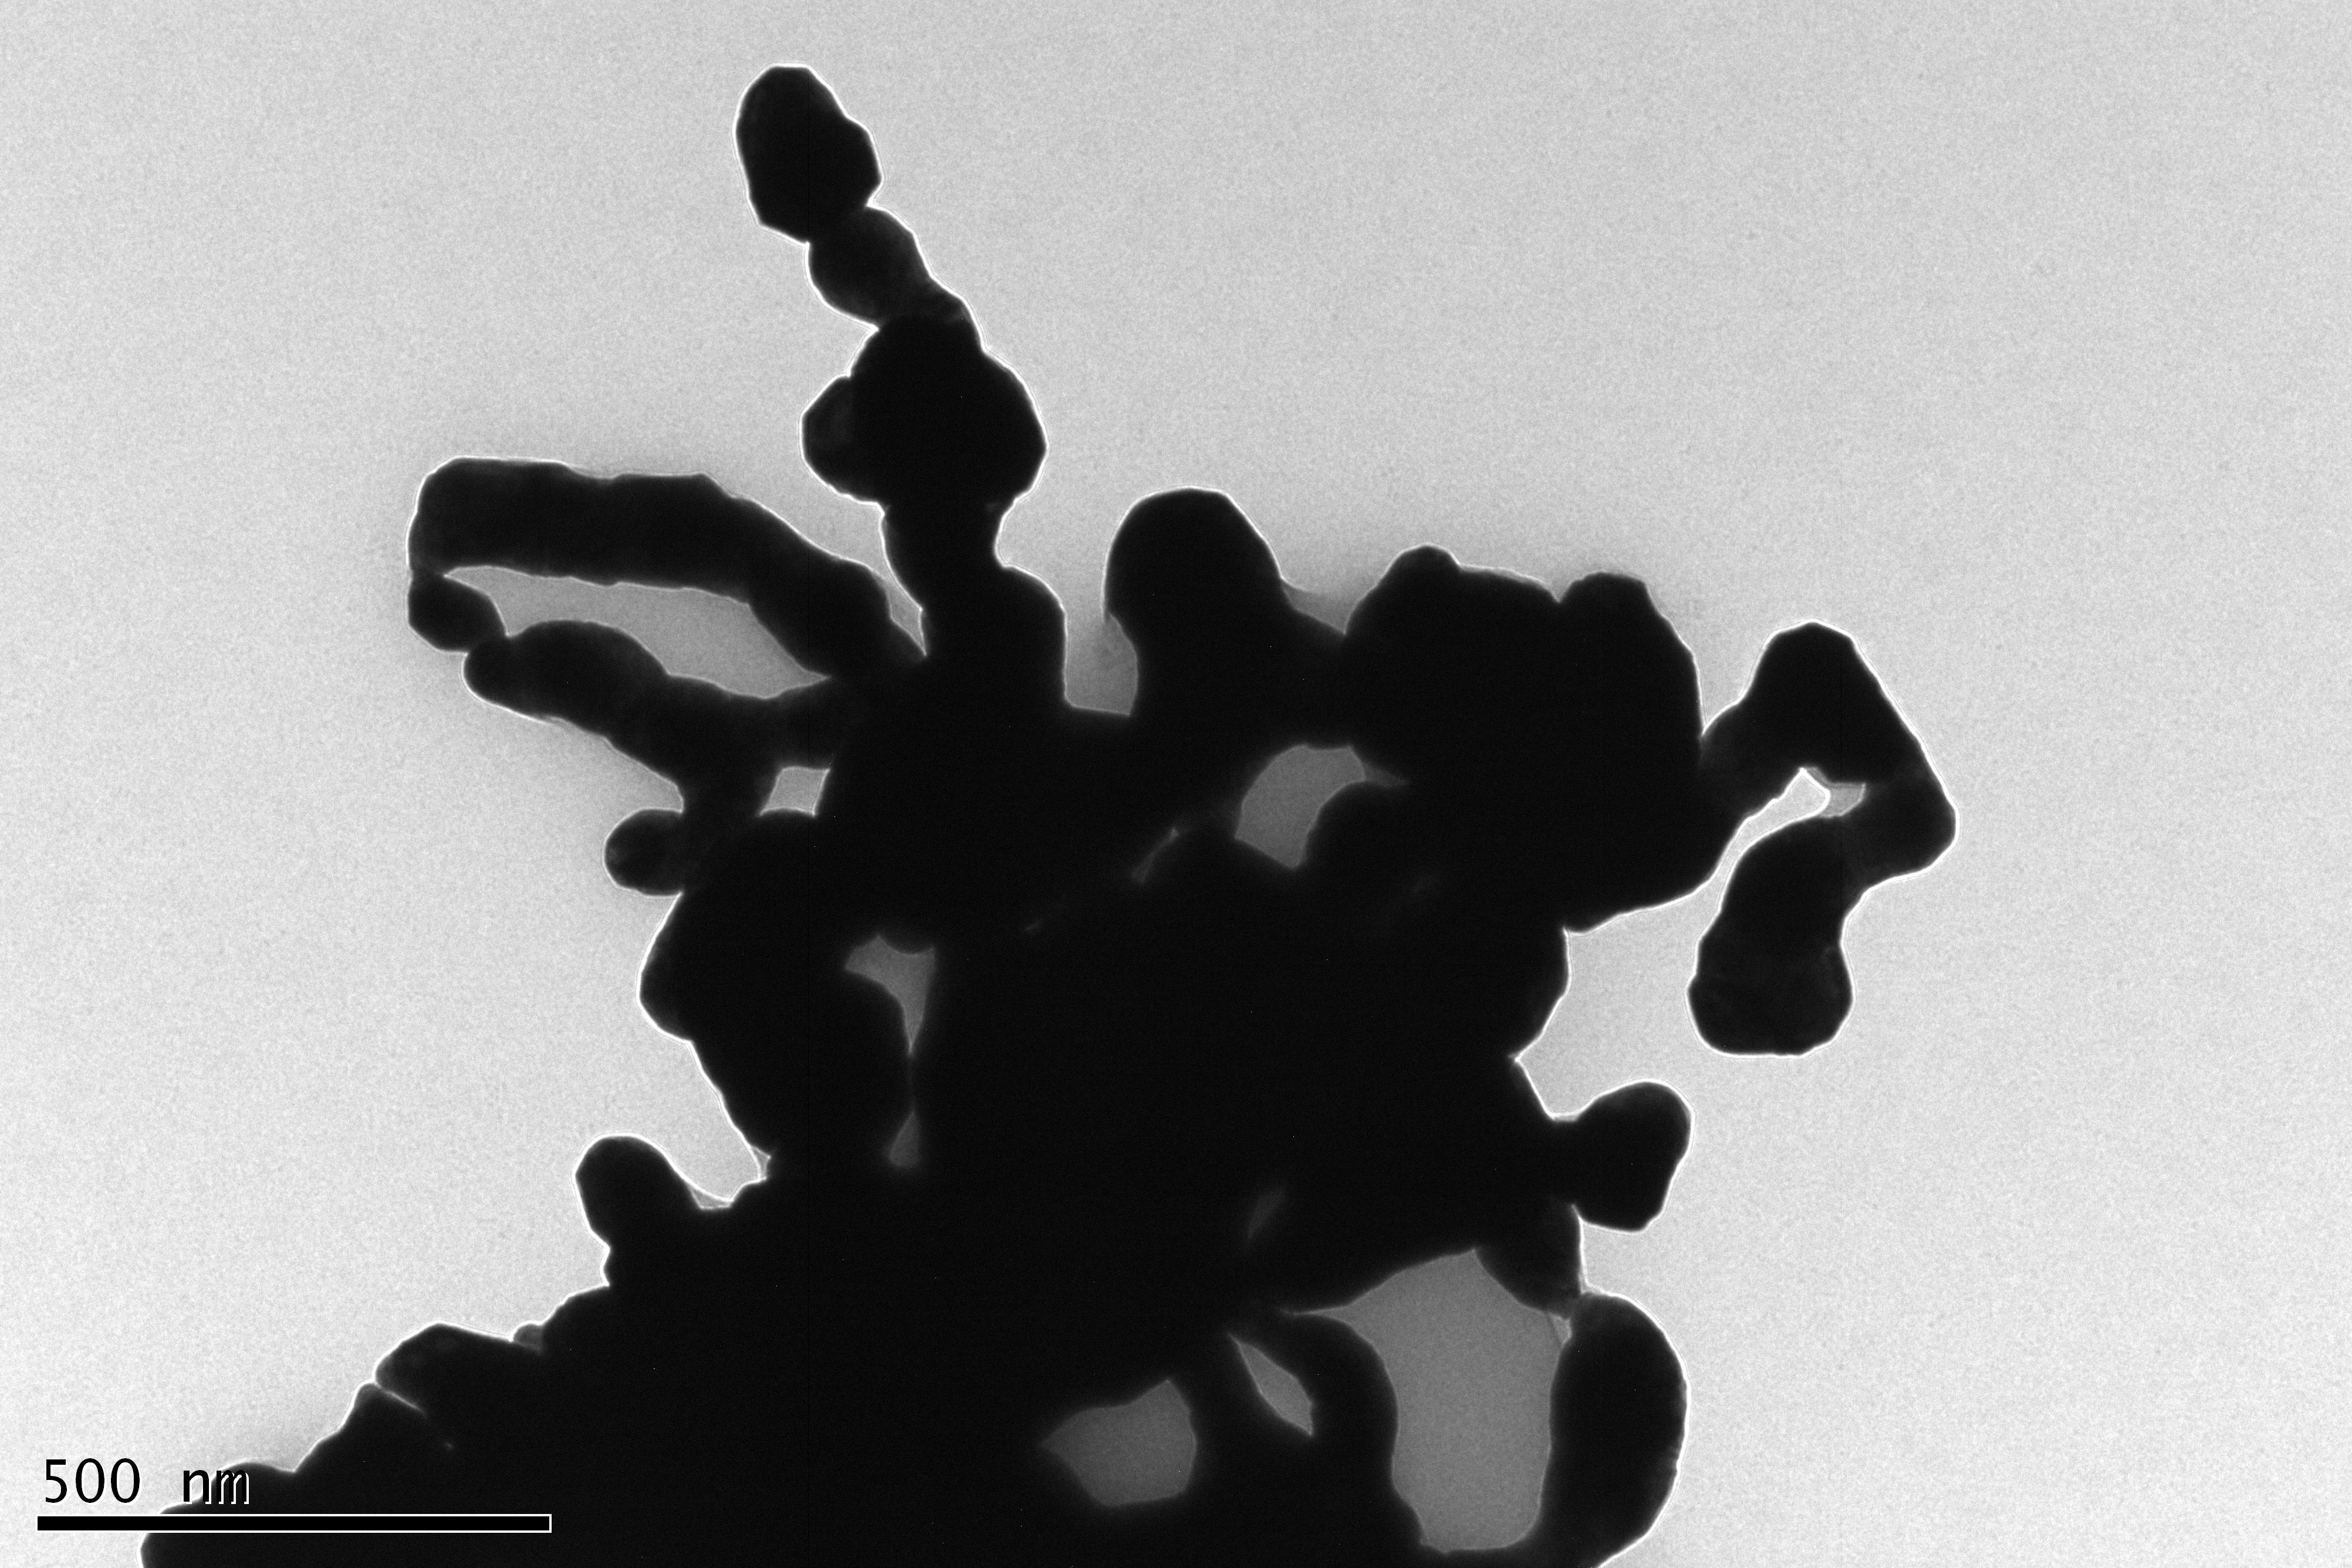
\includegraphics[width=0.45\linewidth]{Bilder/Gel-E-1}}
			\subfloat[\label{fig:Gel-E-2}]{%
				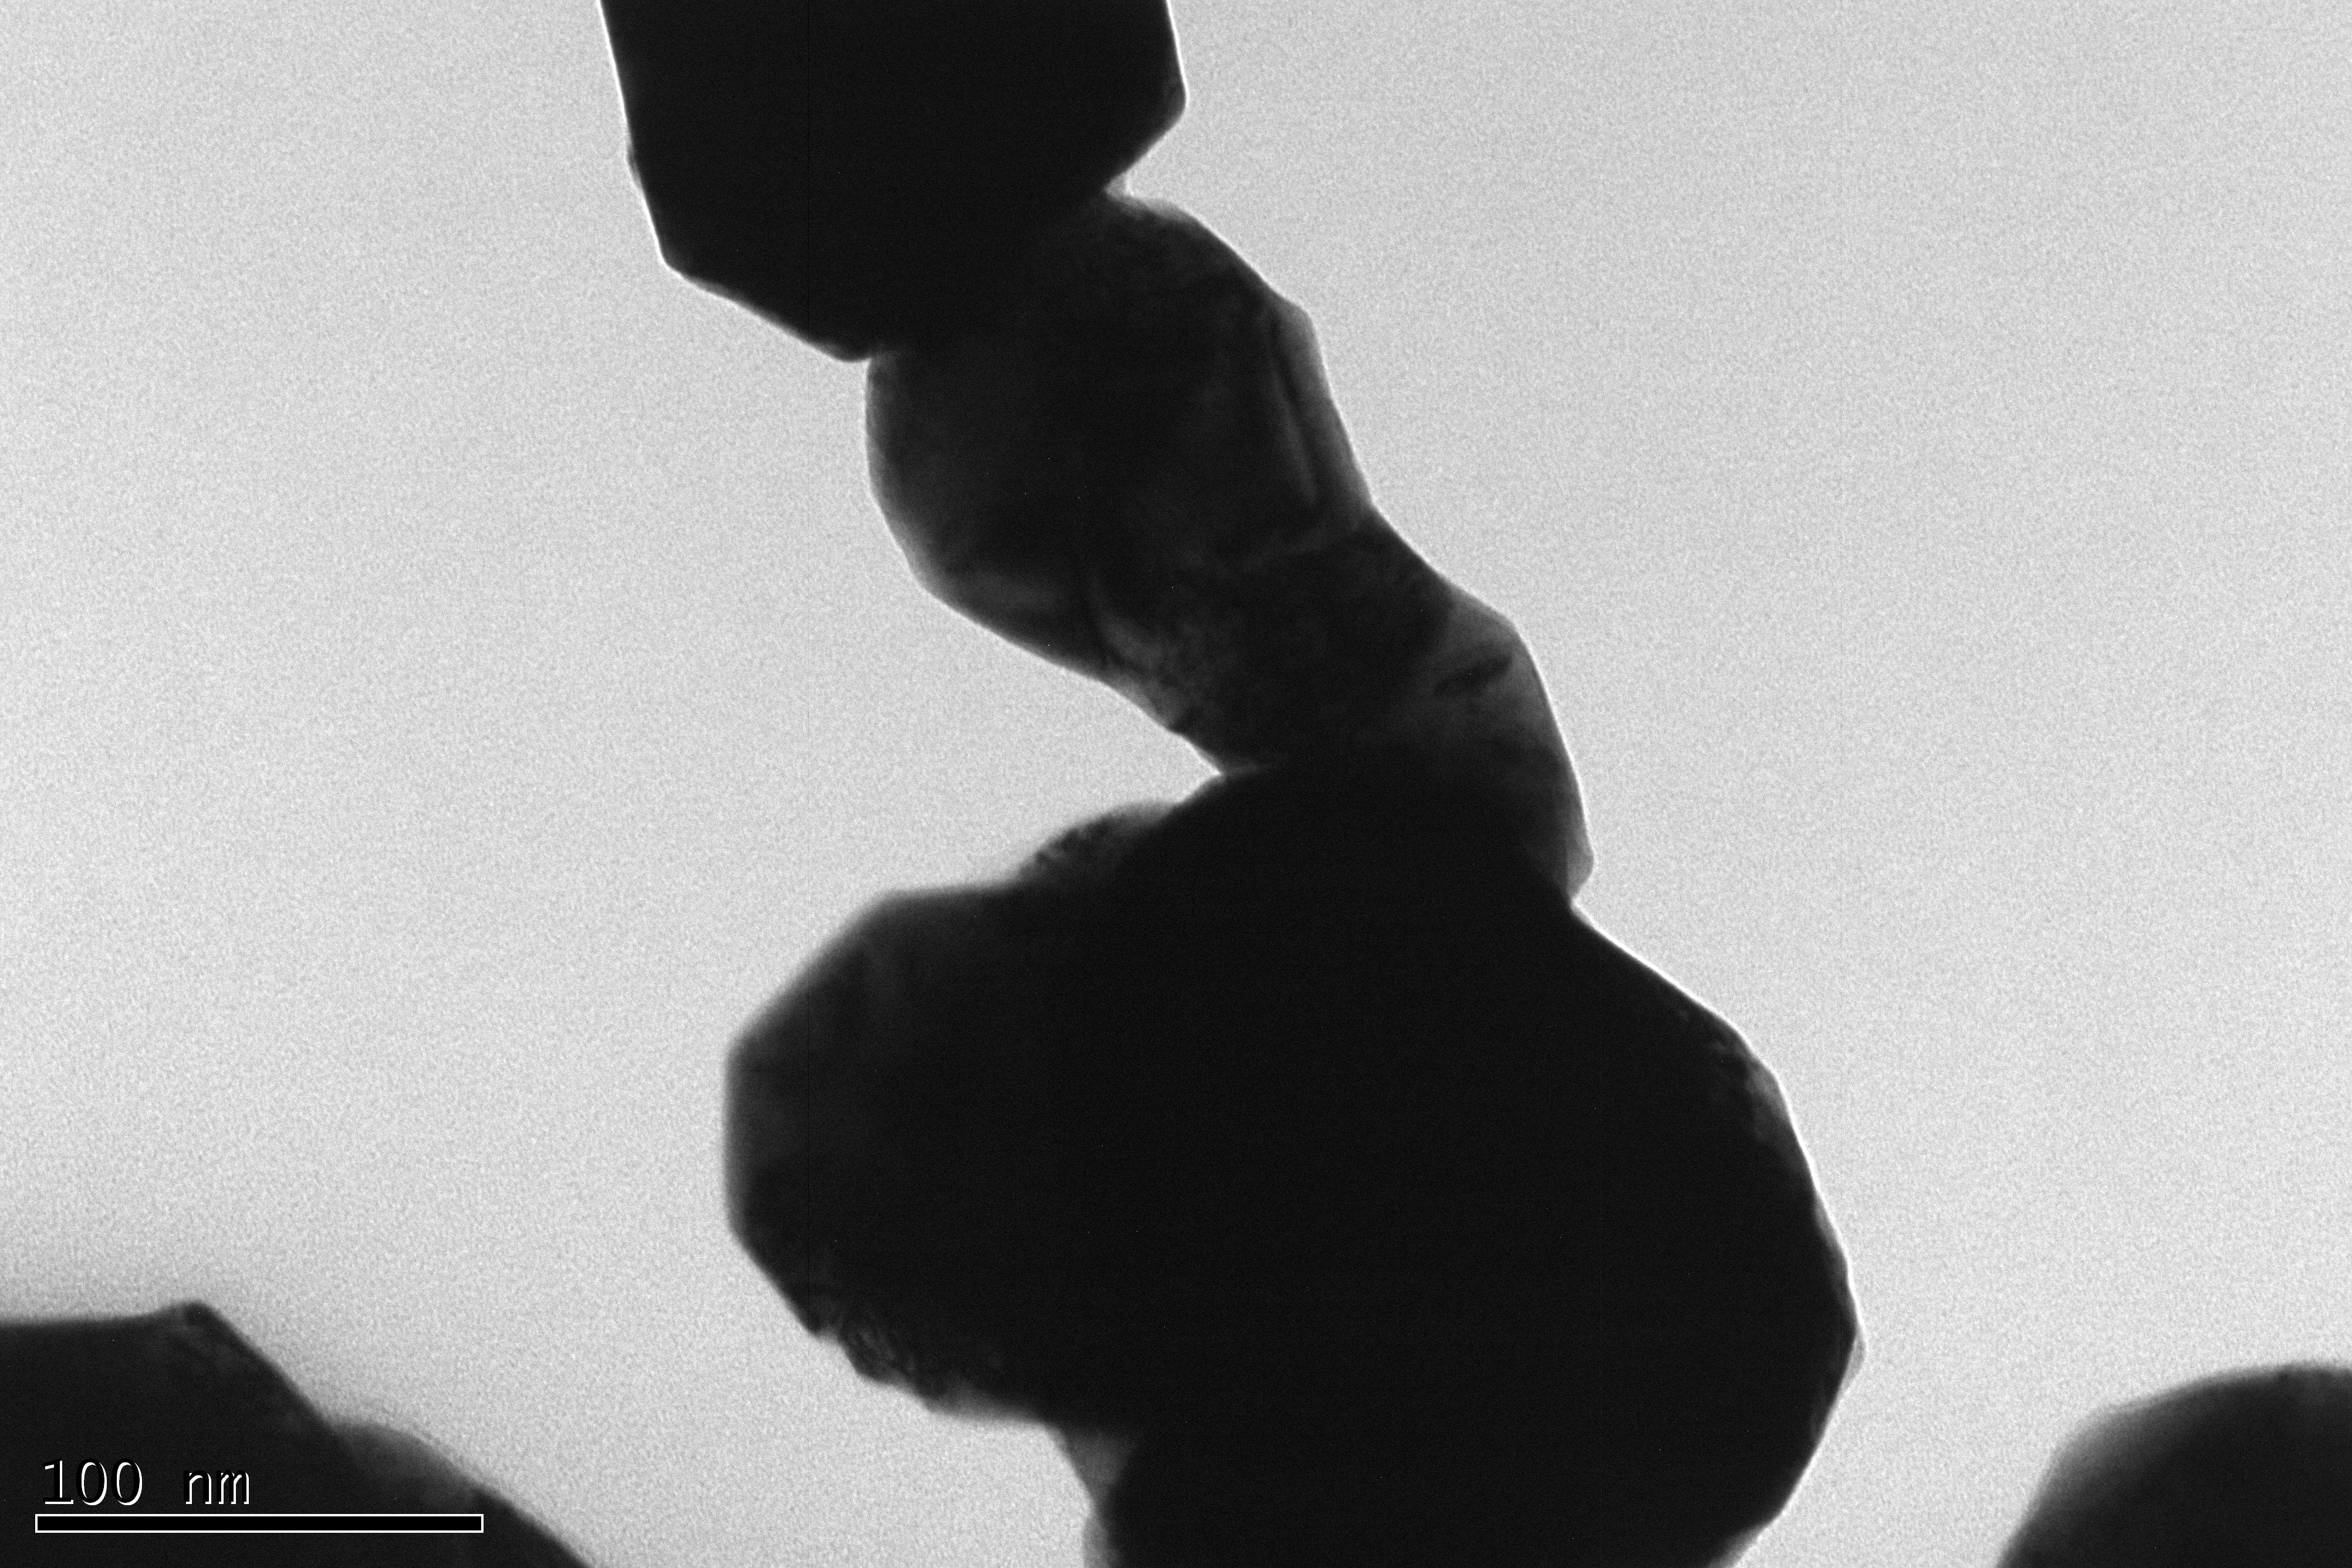
\includegraphics[width=0.45\linewidth]{Bilder/Gel-E-2}}
			\caption{TEM Bilder der Gele aus ethanolischem Ansatz.}
			\label{fig:Gel-E}
		\end{figure}
	
	\subsection{Untersuchung der Metallsulfidsynthese in Anwesenheit von Gelen}
	
	Nachdem die Proben mit Goldpartikeln zeigten, dass bei der thermischen Zersetzung von \ch{Cu[DDTC]2} sich CuS nicht nur getrennt vom Gold bildet, wurde hier getestet ob sich CuS (und später auch CdS und ZnS) an schon vorhandene Gele anlagert bzw. aufwächst und mit welchen Parametern man dieses Verhalten beeinflussen kann.
	Dabei wurde hauptsächlich mit den Gelen aus ethanolischem Ansatz gearbeitet.
	
	Es zeigte sich direkt, dass wie zu erwarten die Gele zusammenschrumpften während des Verdampfungsprozesses.
	Allerdings sind diese Xerogele, wie in \cref{fig:vn} gezeigt, nicht so stark geschrumpft, wie es von anderen Gelen bekannt ist, was mit der relativ groben Struktur der Gele und verhältnismäßig kleinen Zwischenräumen, die kollabieren können, zusammenhängt.
	
	
	\begin{figure}[H]
	\centering
	\subfloat[\label{fig:vorher}]{%
		\includegraphics[width=0.45\linewidth]{Bilder/Gel-E-vorher}}
	\subfloat[\label{fig:nachher}]{%
		\includegraphics[width=0.45\linewidth]{Bilder/Gel-E-nachher}}
	\caption{Vergleich der Gele \emph{(a)}: vor und \emph{(b)}: nach der Erhitzung.}
	\label{fig:vn}
	\end{figure} 


	Die TEM-Aufnahmen des Gels, das mit \ch{Cu[DDTC]2} bei \SI{290}{\degreeCelsius} bearbeitet wurde, die in \cref{fig:E-Cu} gezeigt sind, zeigen, dass sich CuS am Gel gebildet hat.
	Von einer kompletten Schale ist es noch weit entfernt, aber es zeigt, dass es möglich ist, mittels  thermischer Zersetzung von \ch{Cu[DDTC]2}, das daraus entstehende CuS daran anzulagern.
	
	\begin{figure}[H]
		\centering
		\subfloat[\label{fig:Gel-E-Cu_1}]{%
			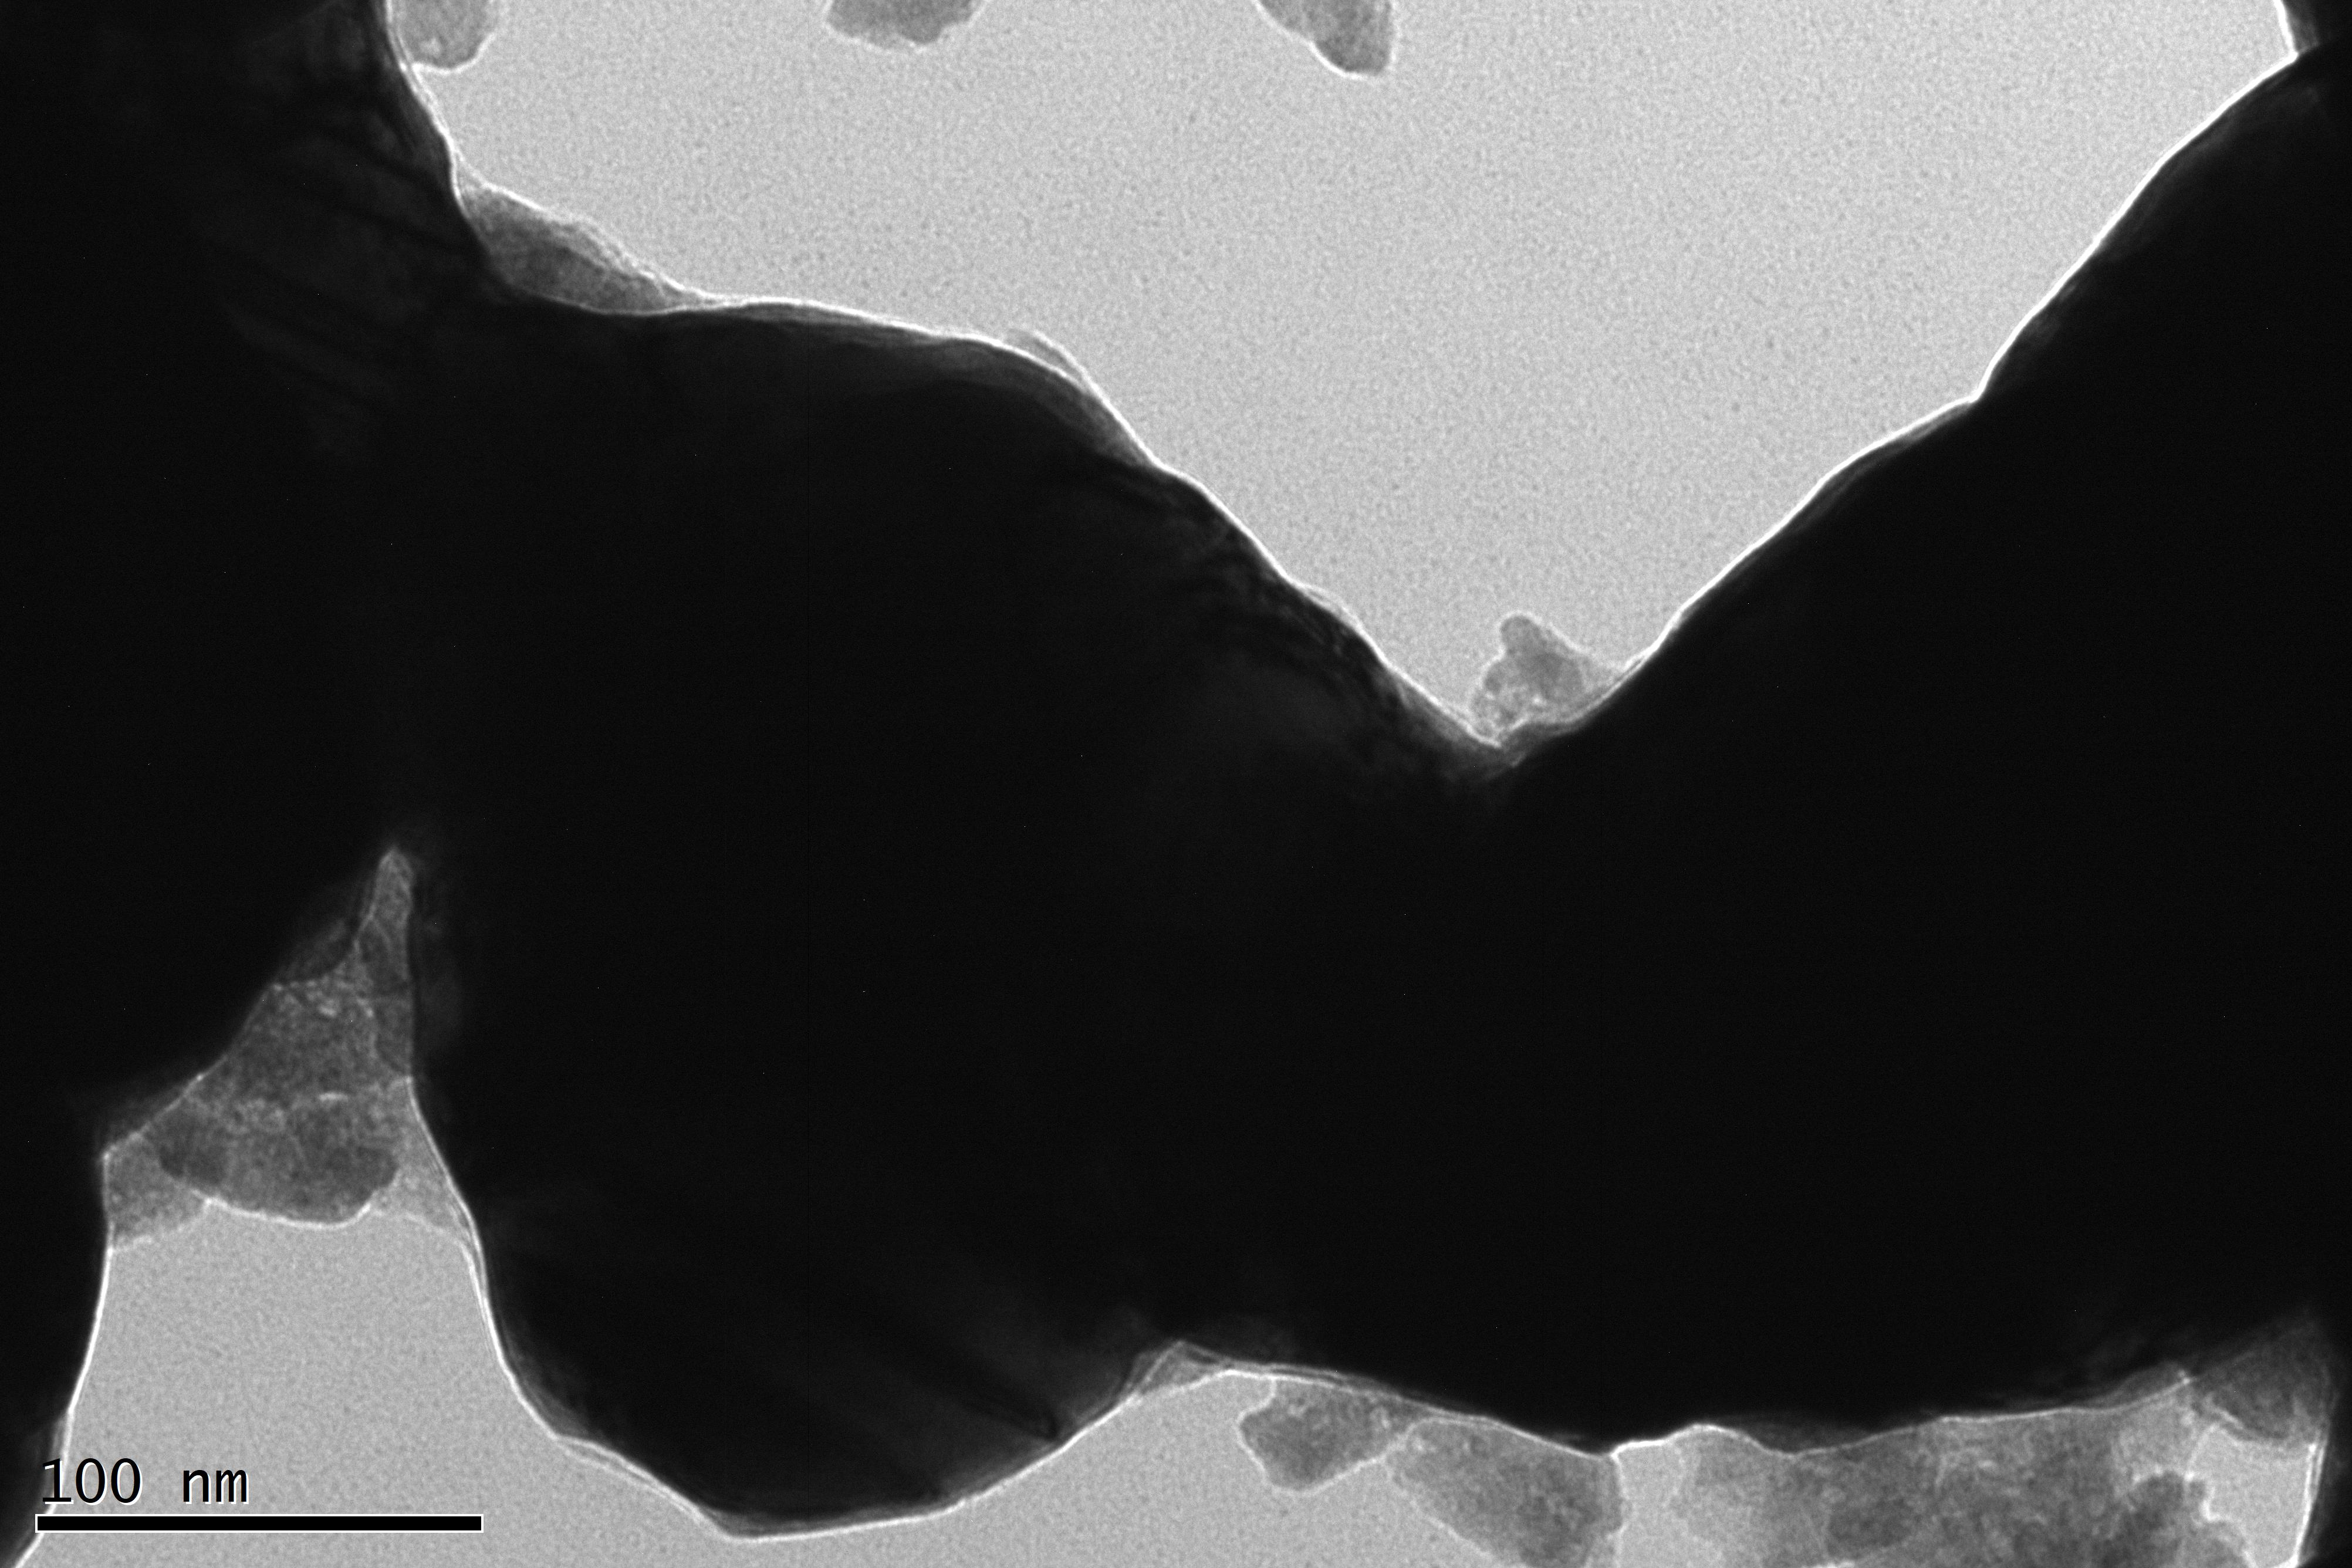
\includegraphics[width=0.45\linewidth]{Bilder/Gel-E-Cu_1}}
		\subfloat[\label{fig:Gel-E-Cu_2}]{%
			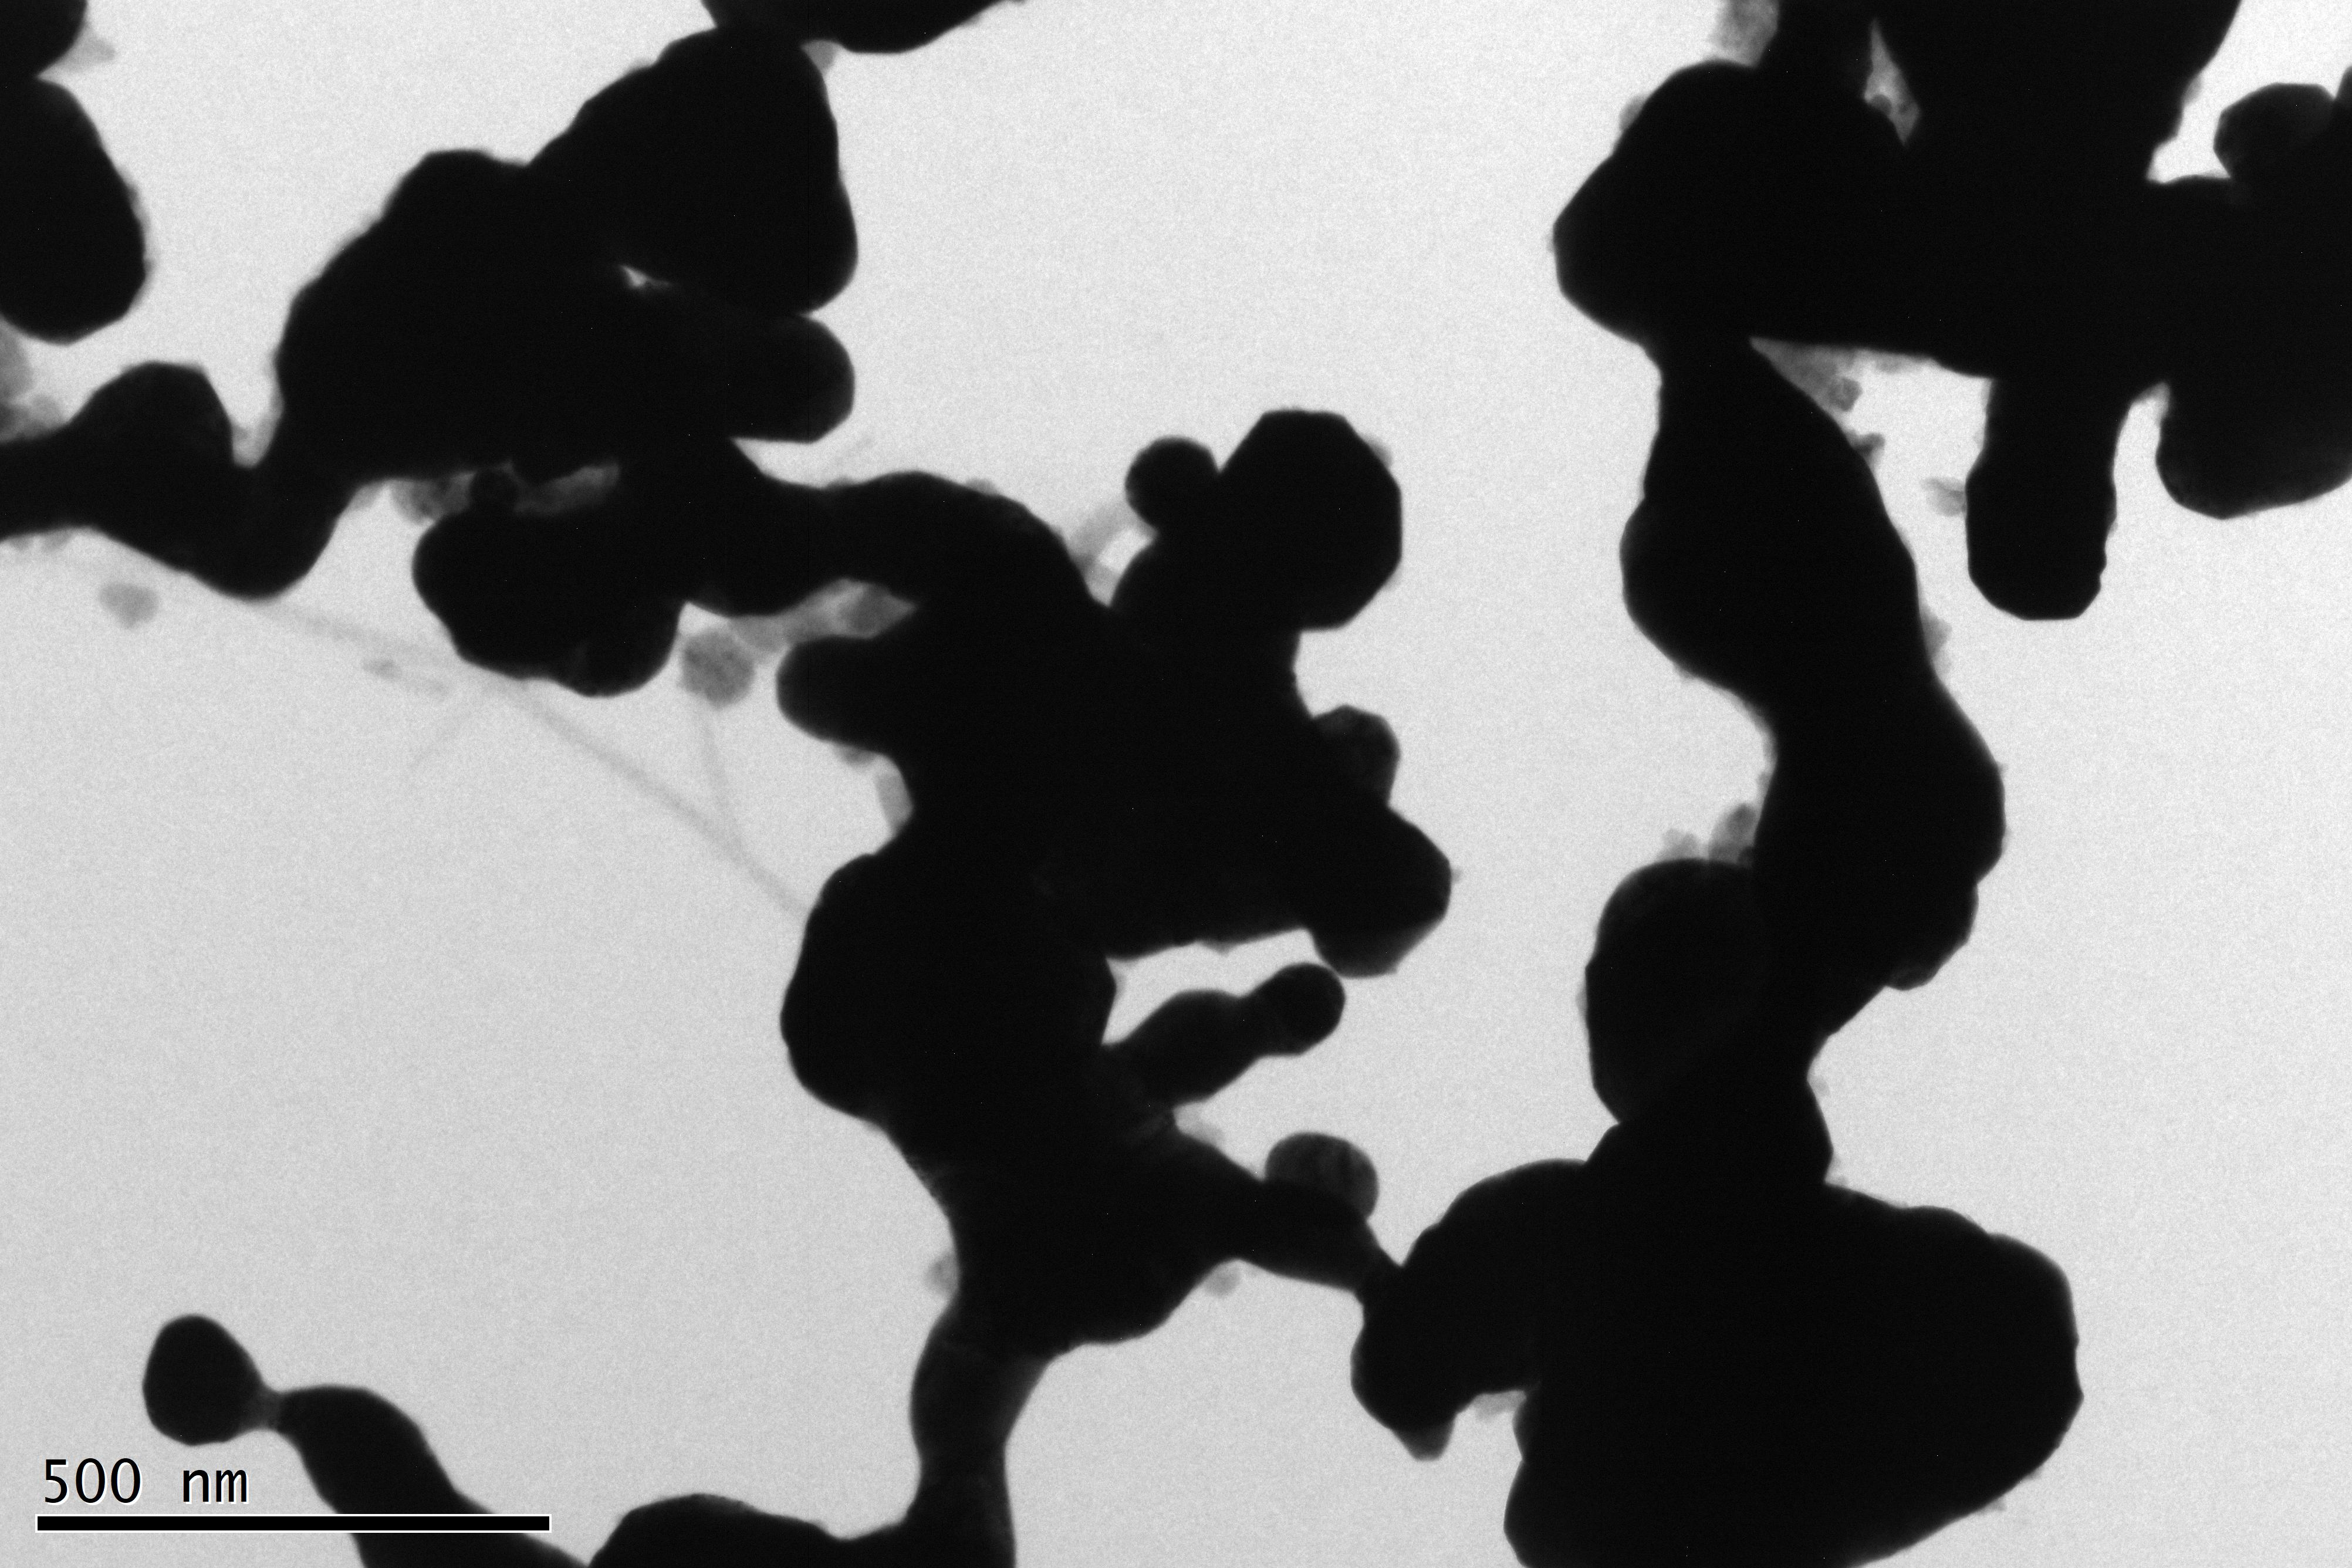
\includegraphics[width=0.45\linewidth]{Bilder/Gel-E-Cu_2}}
		\caption{TEM von einem ethanolischen Au-Gel mit CuS.}
		\label{fig:E-Cu}
	\end{figure}


	\subsubsection{Einfluss der Reaktionstemperatur}
		
		Bei den getesteten Gelen, die mit geringeren Temperaturen behandelt wurden, zeigt sich, dass bei geringeren Temperaturen, sich CuS wenig bis gar nicht an den Gelen bildet, wie in \cref{fig:Gel-E-Temp} gezeigt wird.
		Die Temperatur von \SI{250}{\degreeCelsius} scheint also nicht ausreichend um CuS aus der thermischen Zersetzung von \ch{Cu[DDTC]2} zu gewinnen, da auch neben den Gelen kein CuS gefunden werden konnte.
		Aus diesem Grund wurde auch bei späteren Versuchen nie von den \SI{290}{\degreeCelsius} abgewichen.
		\begin{figure}[H]
			\centering
			\subfloat[\label{fig:Gel-E-200C}]{%
				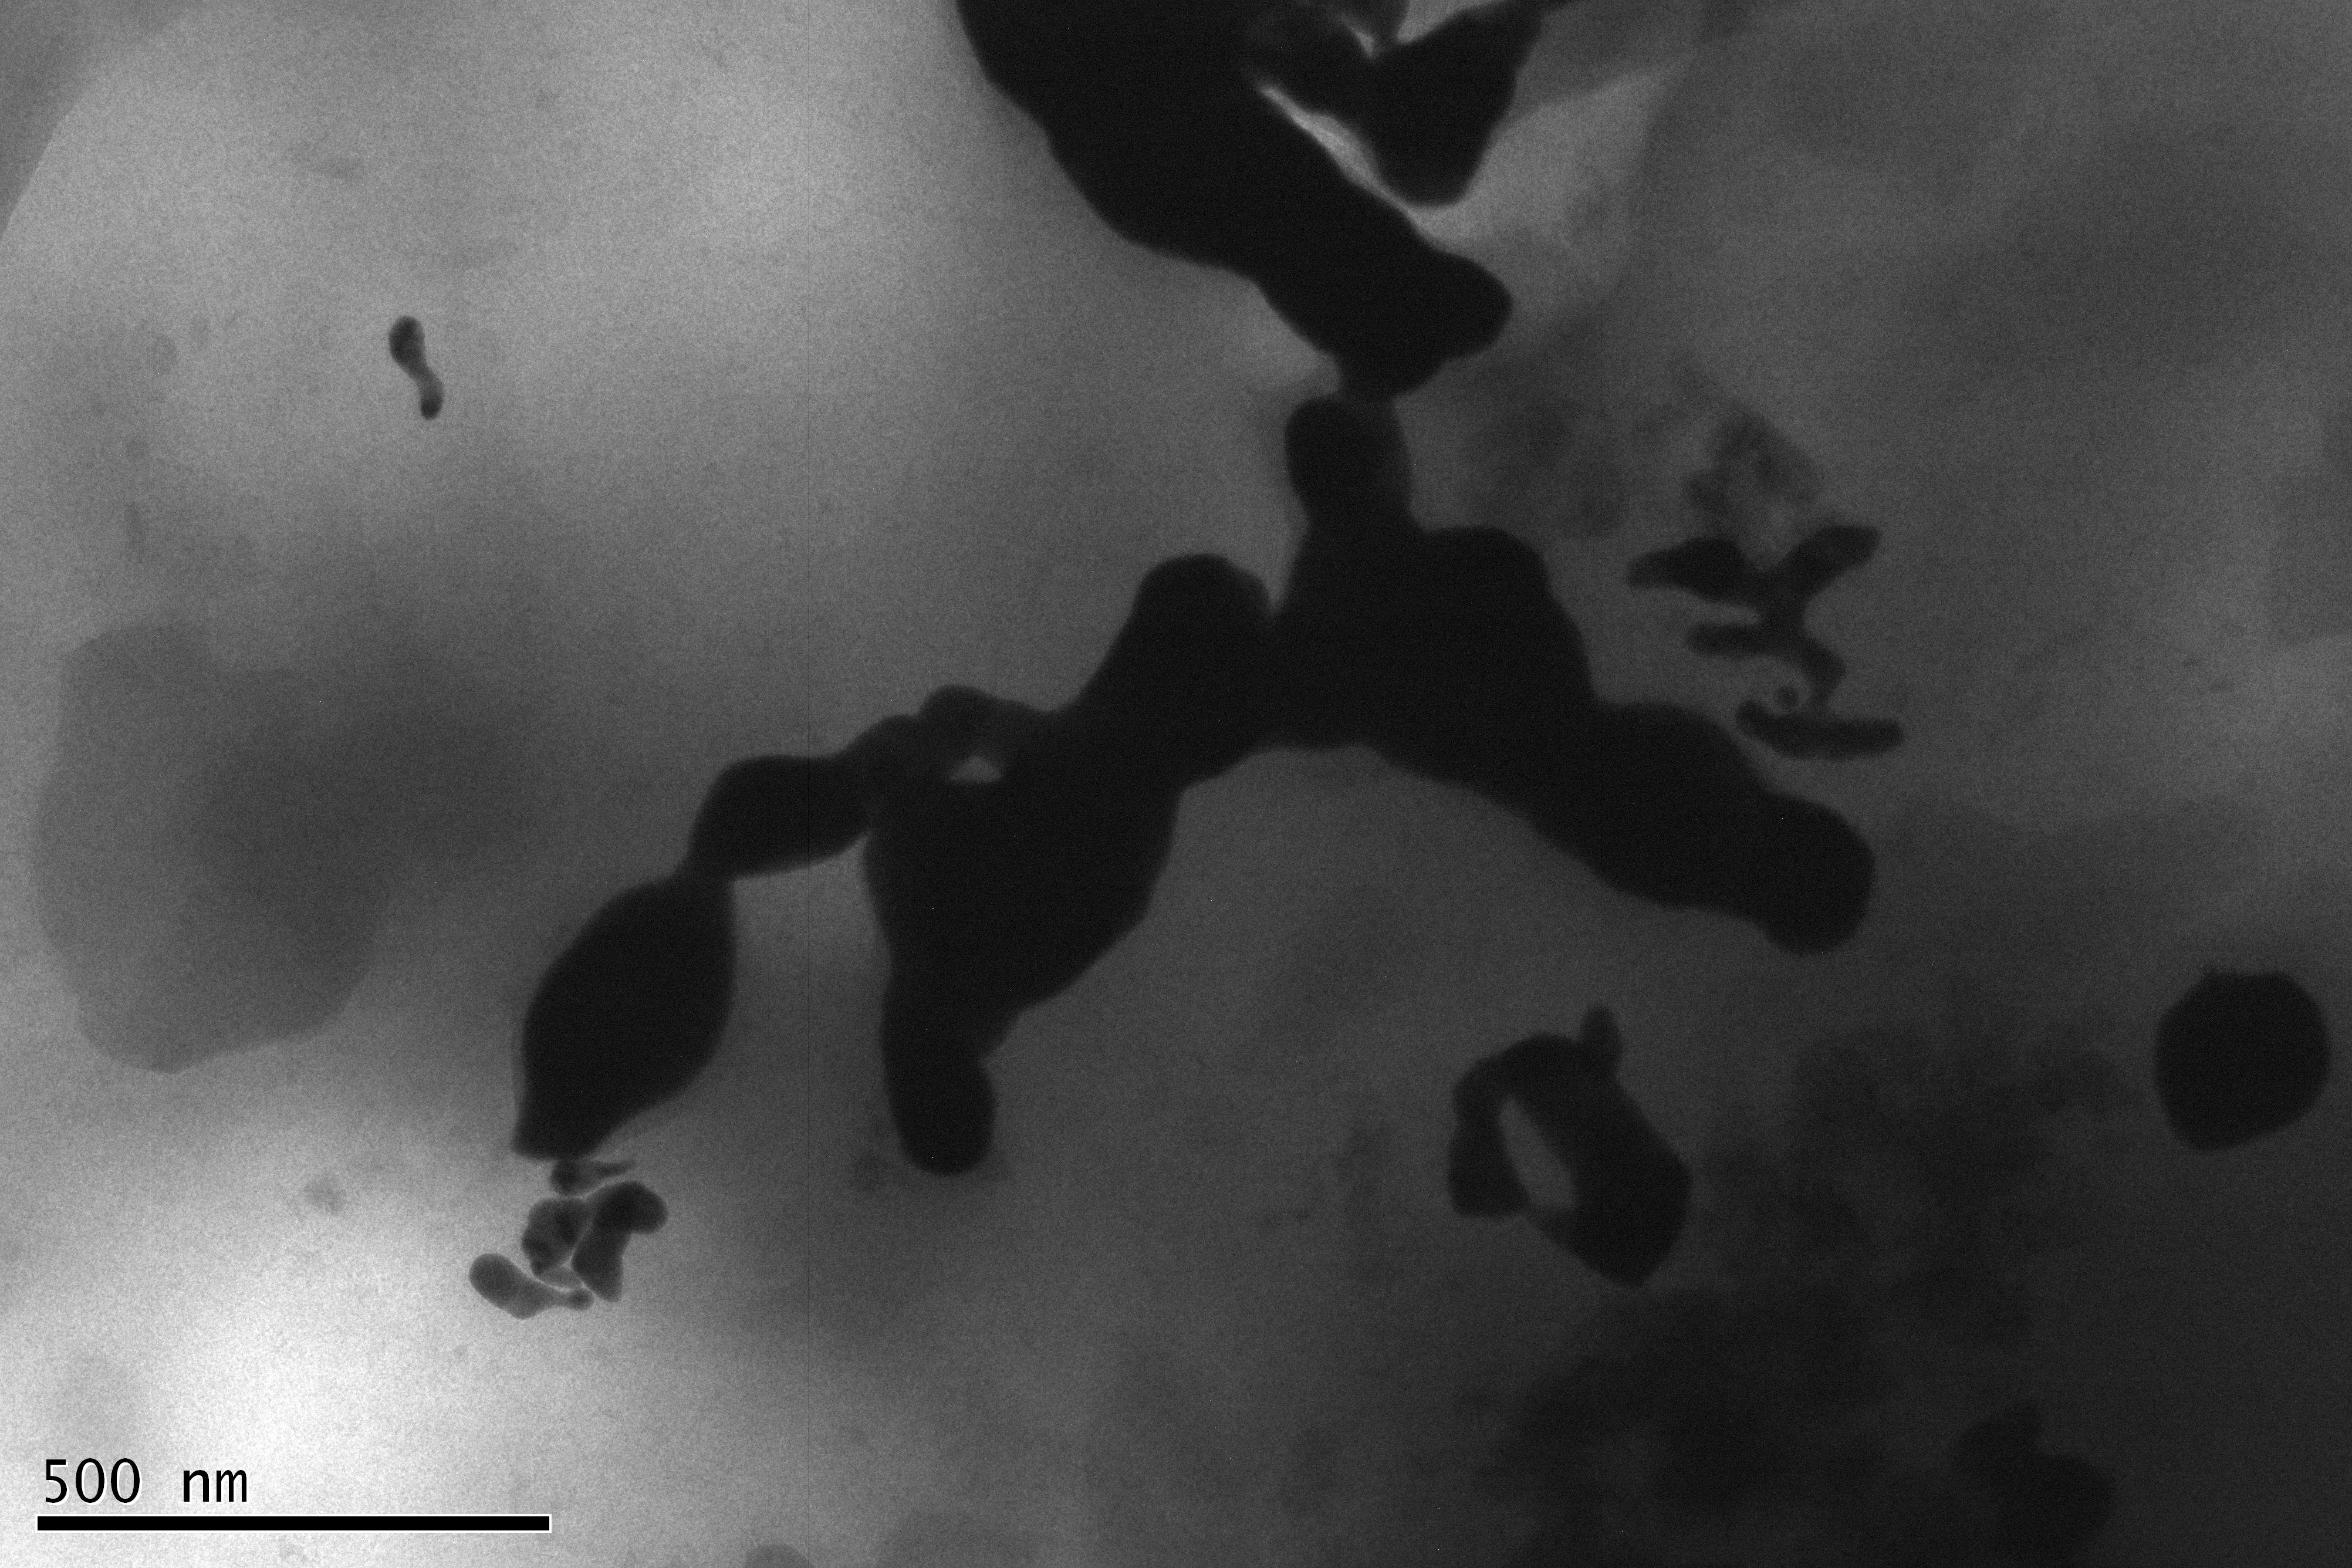
\includegraphics[width=0.45\linewidth]{Bilder/Gel-E-200C}}
			\subfloat[\label{fig:Gel-E-250C}]{%
				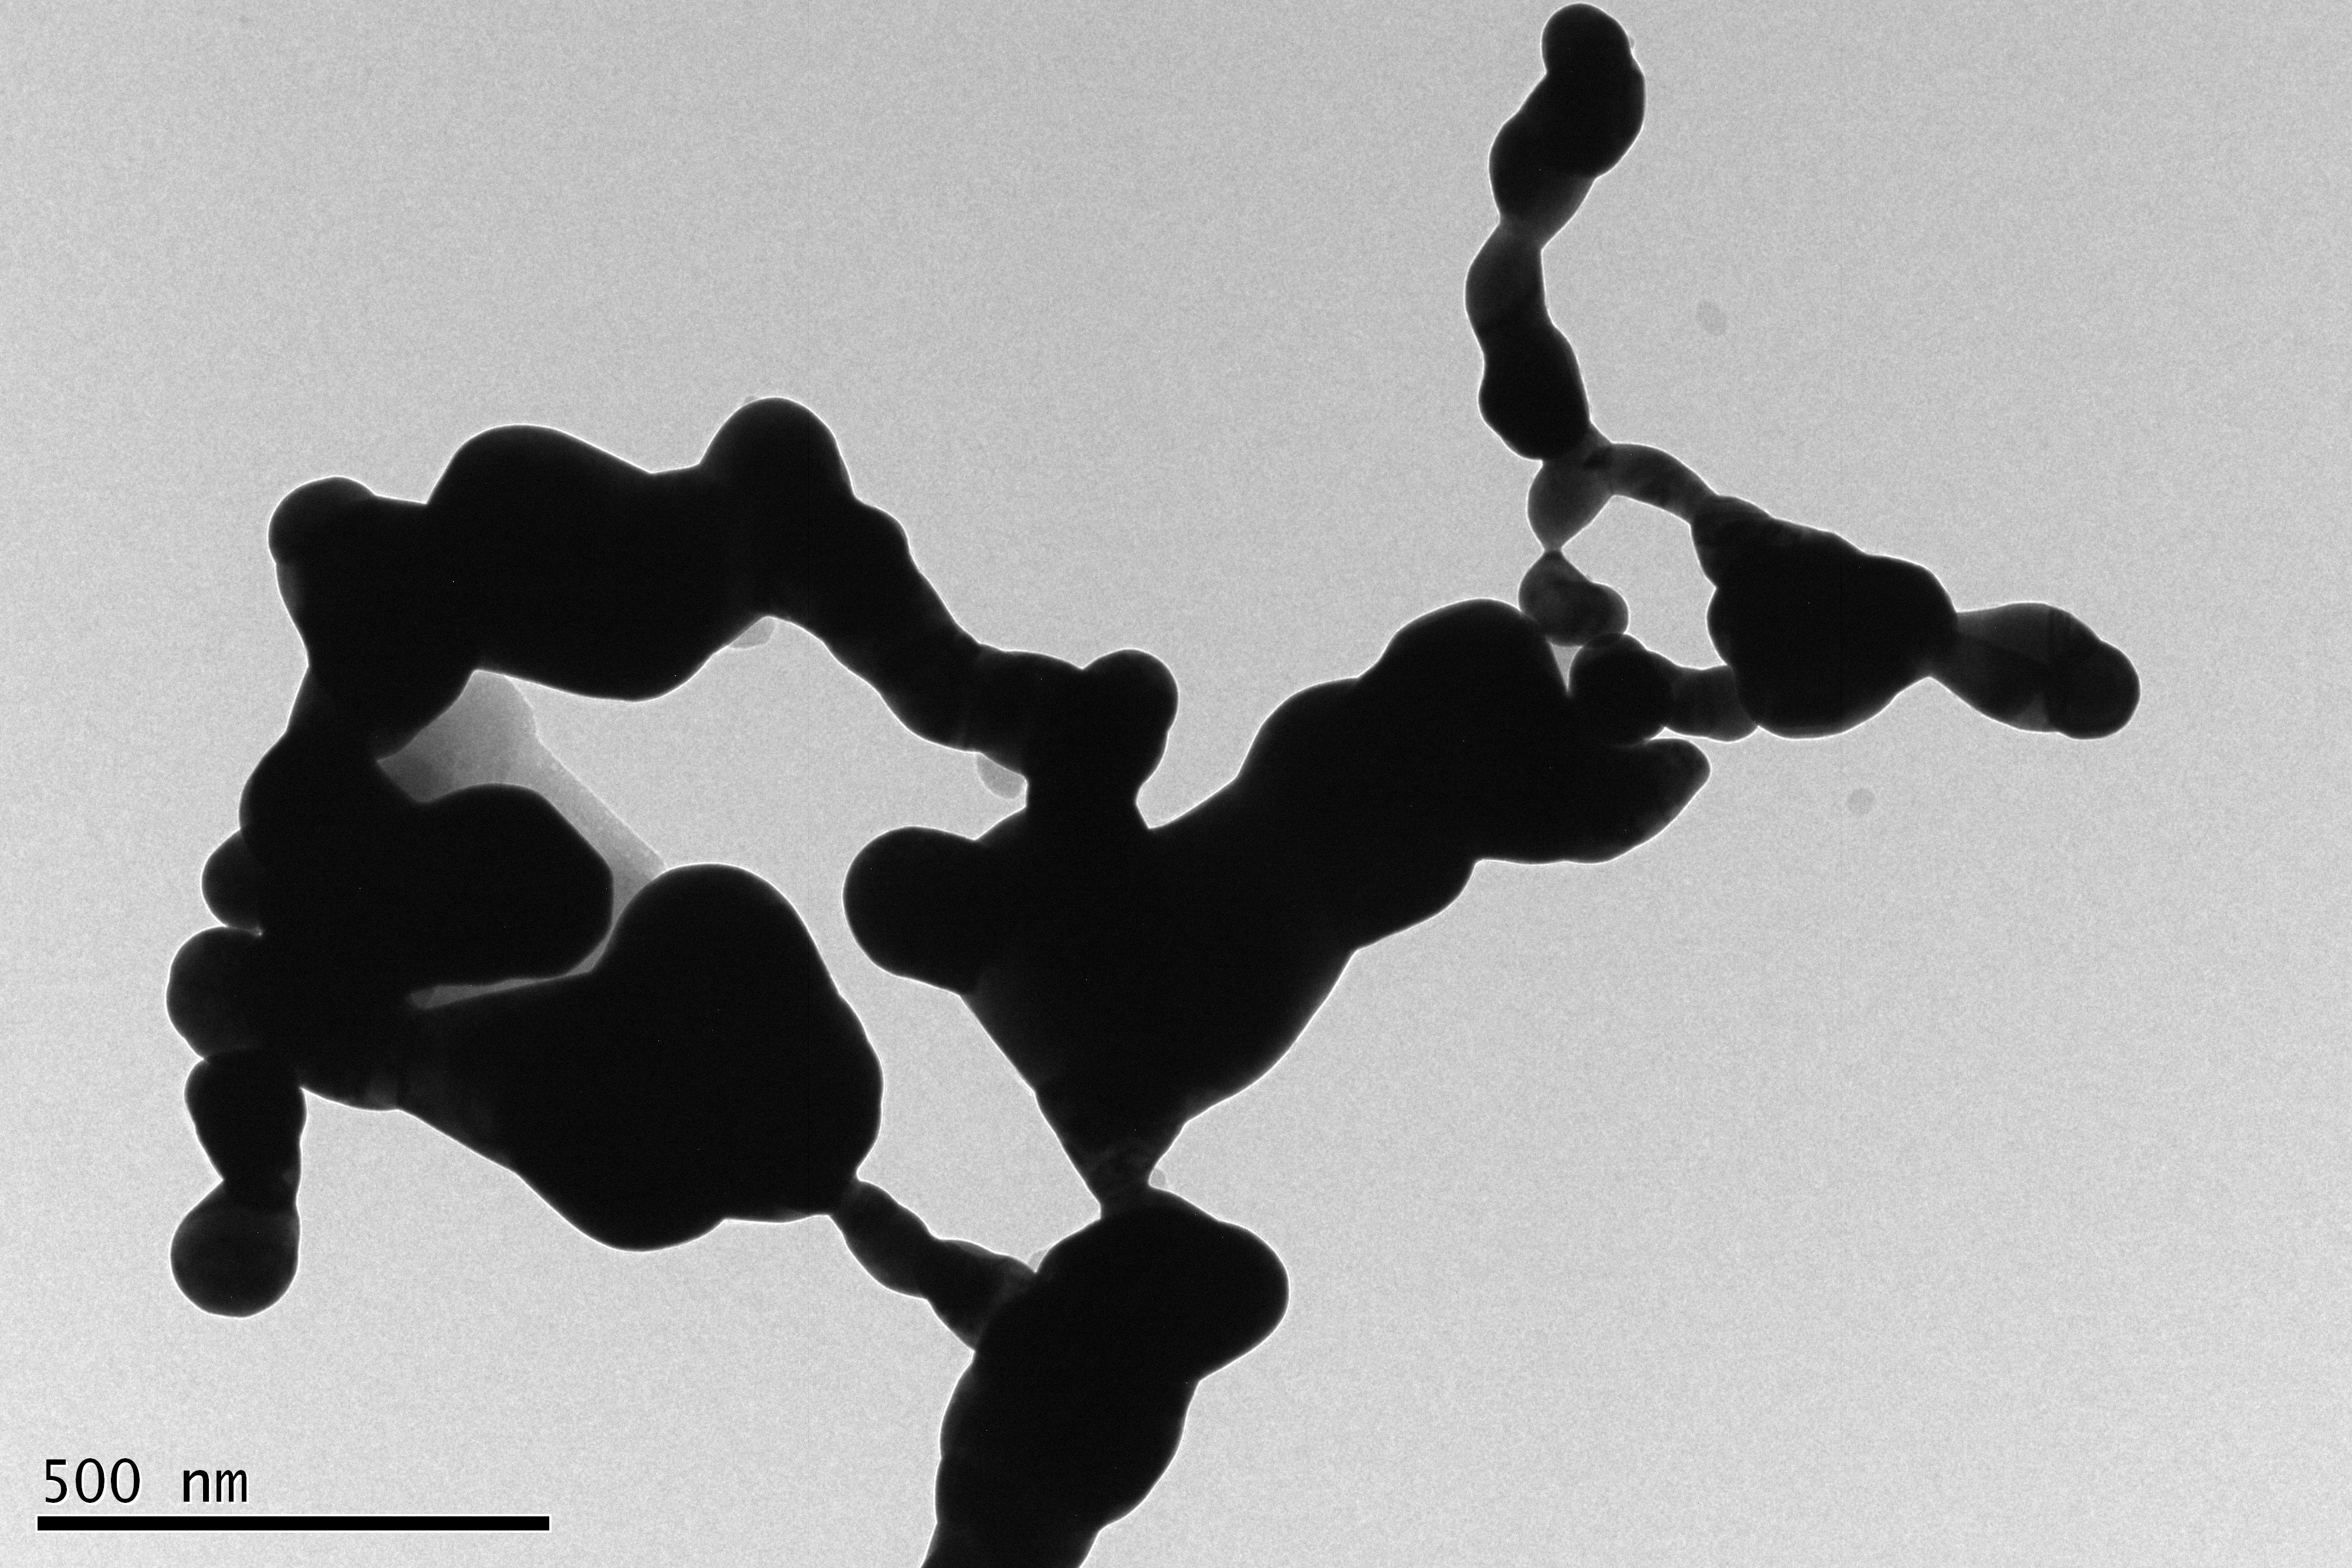
\includegraphics[width=0.45\linewidth]{Bilder/Gel-E-250C}}
			\caption{Gele nach der Reaktion mit \ch{Cu[DDTC]2} bei \emph{(a)}: \SI{200}{\degreeCelsius} und \emph{(b)}: \SI{250}{\degreeCelsius}.}
			\label{fig:Gel-E-Temp}
		\end{figure}
	
	\subsubsection{Variation des Kations}
	
		Da es ein Ziel war ein möglichst variablen Mechanismus für das Aufwachsen zu entwickeln, wurde neben \ch{Cu[DDTC]2} auch die gleiche Reaktion mit \ch{Cd[DDTC]2} und \ch{Zn[DDTC]2} untersucht.
		
		Im Gegensatz zum \ch{Cu[DDTC]2} zeigt sich bei gleichem Versuchsaufbau und Durchführung bei \ch{Cd[DDTC]2} ein deutlich anderes Bild.
		es wurden hier nicht nur einzelne  kleine Zwischenräume mit CdS bedeckt, sondern es kommt zu einer fast kompletten Ummantelung des Gels wie in \cref{fig:Gel-E-CdS} zu erkennen ist.
		Allerdings hat sich auch ein Teil des CdS neben dem Gel gebildet. 
		Dies ist sowohl in den TEM-Aufnahmen zu erkennen aber auch schon mit bloßem Auge lässt sich die typische Gelbfärbung vom CdS am kompletten Boden des Reaktionsgefäßes auch neben dem Gel erkennen, wie in \cref{fig:Foto-CdS} gezeigt.
		\begin{figure}[H]
			\centering
			\subfloat[\label{fig:Gel-E-CdS_1}]{%
				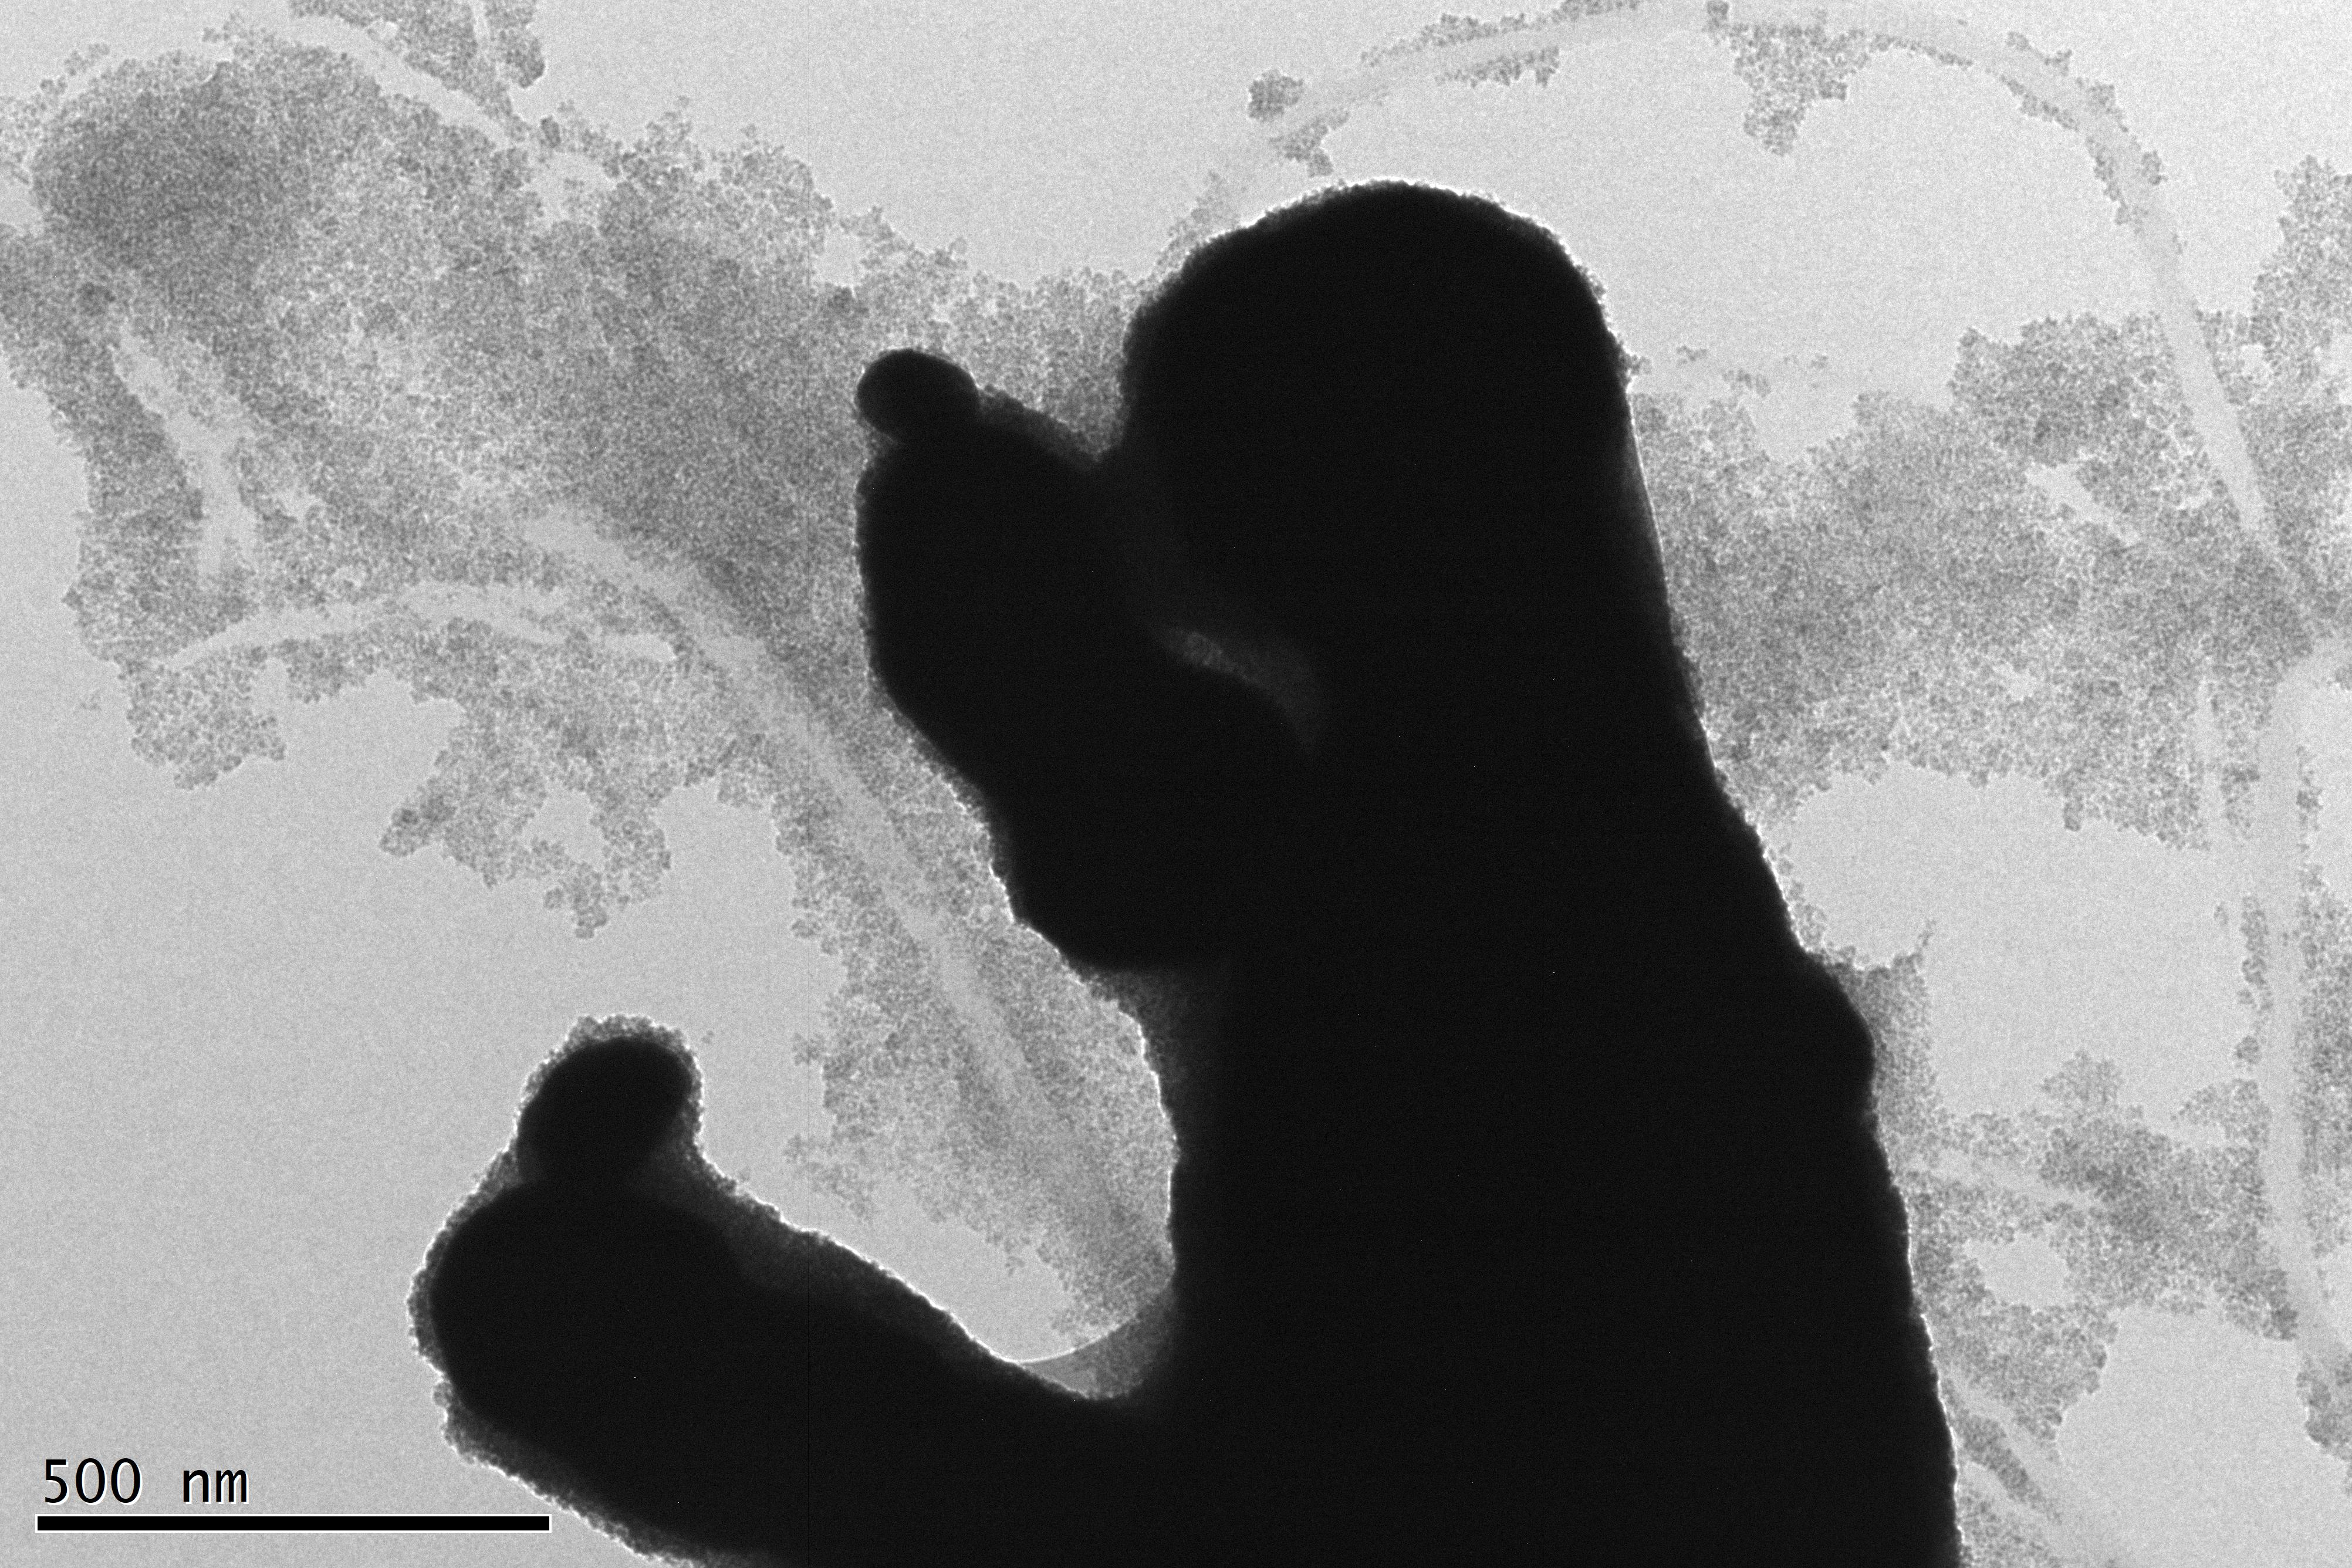
\includegraphics[width=0.33\linewidth]{Bilder/Gel-E-CdS_1}}
			\subfloat[\label{fig:Gel-E-CdS_2}]{%
				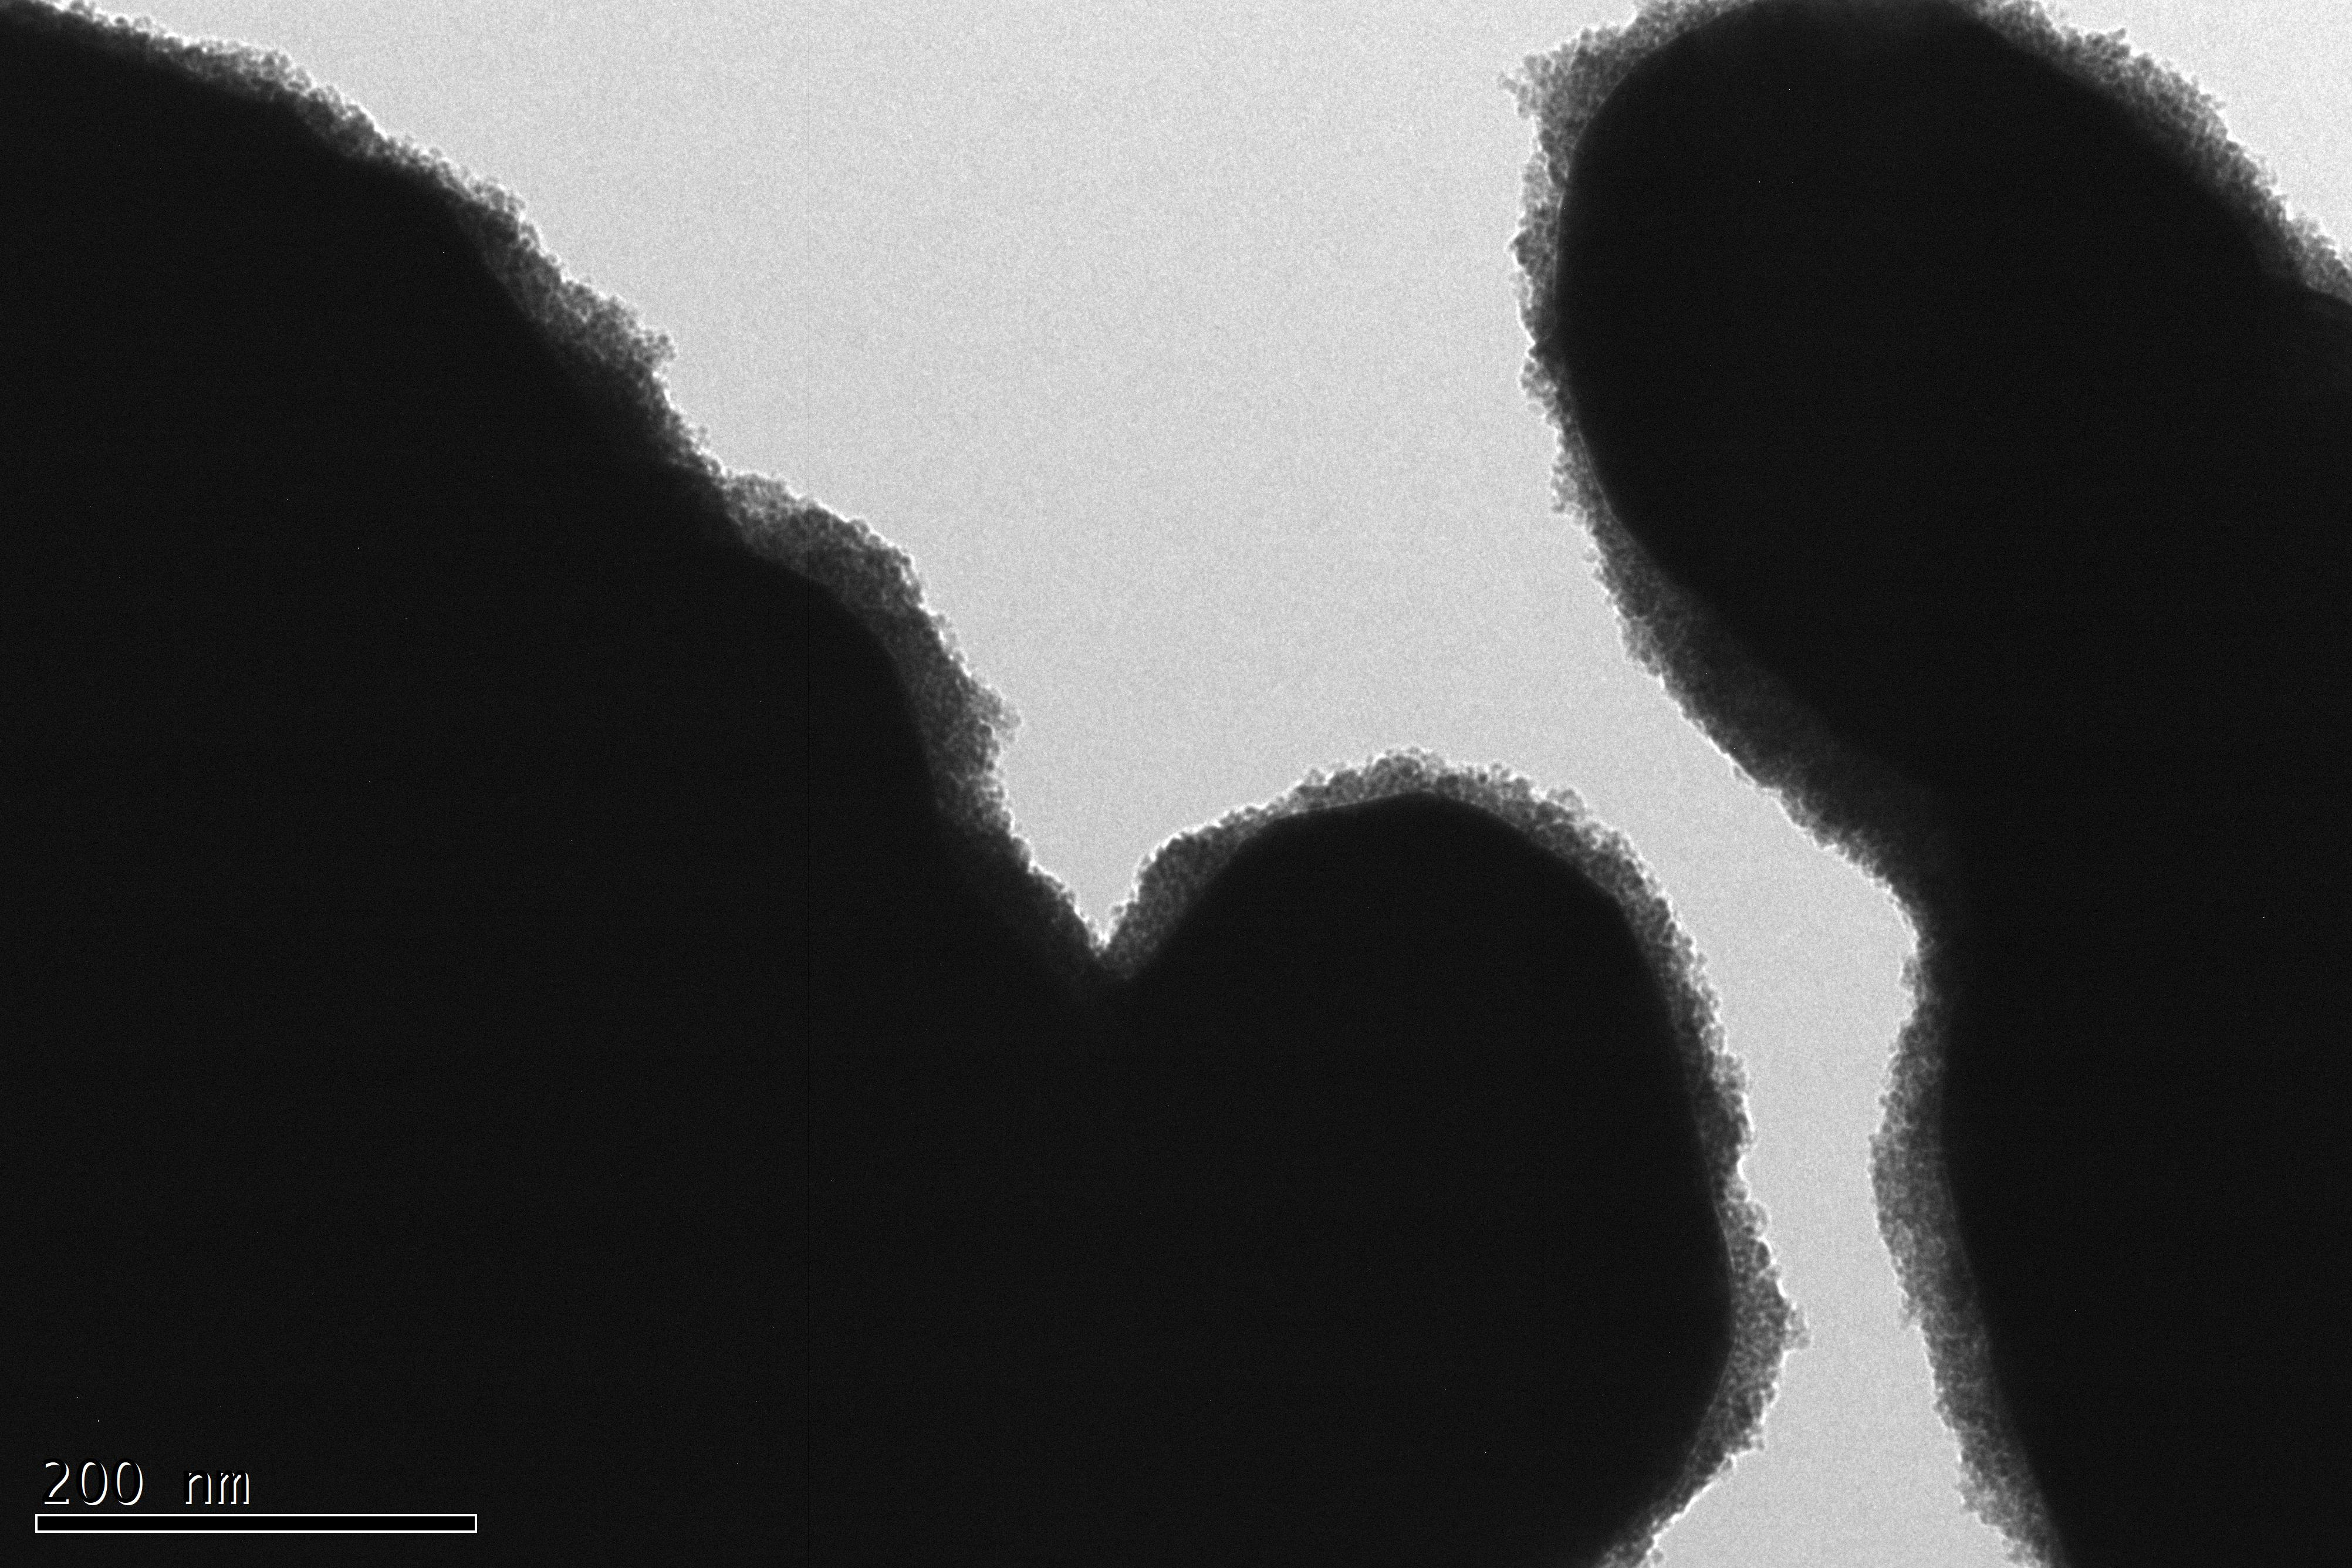
\includegraphics[width=0.33\linewidth]{Bilder/Gel-E-CdS_2}}
			\subfloat[\label{fig:Gel-E-CdS_3}]{%
				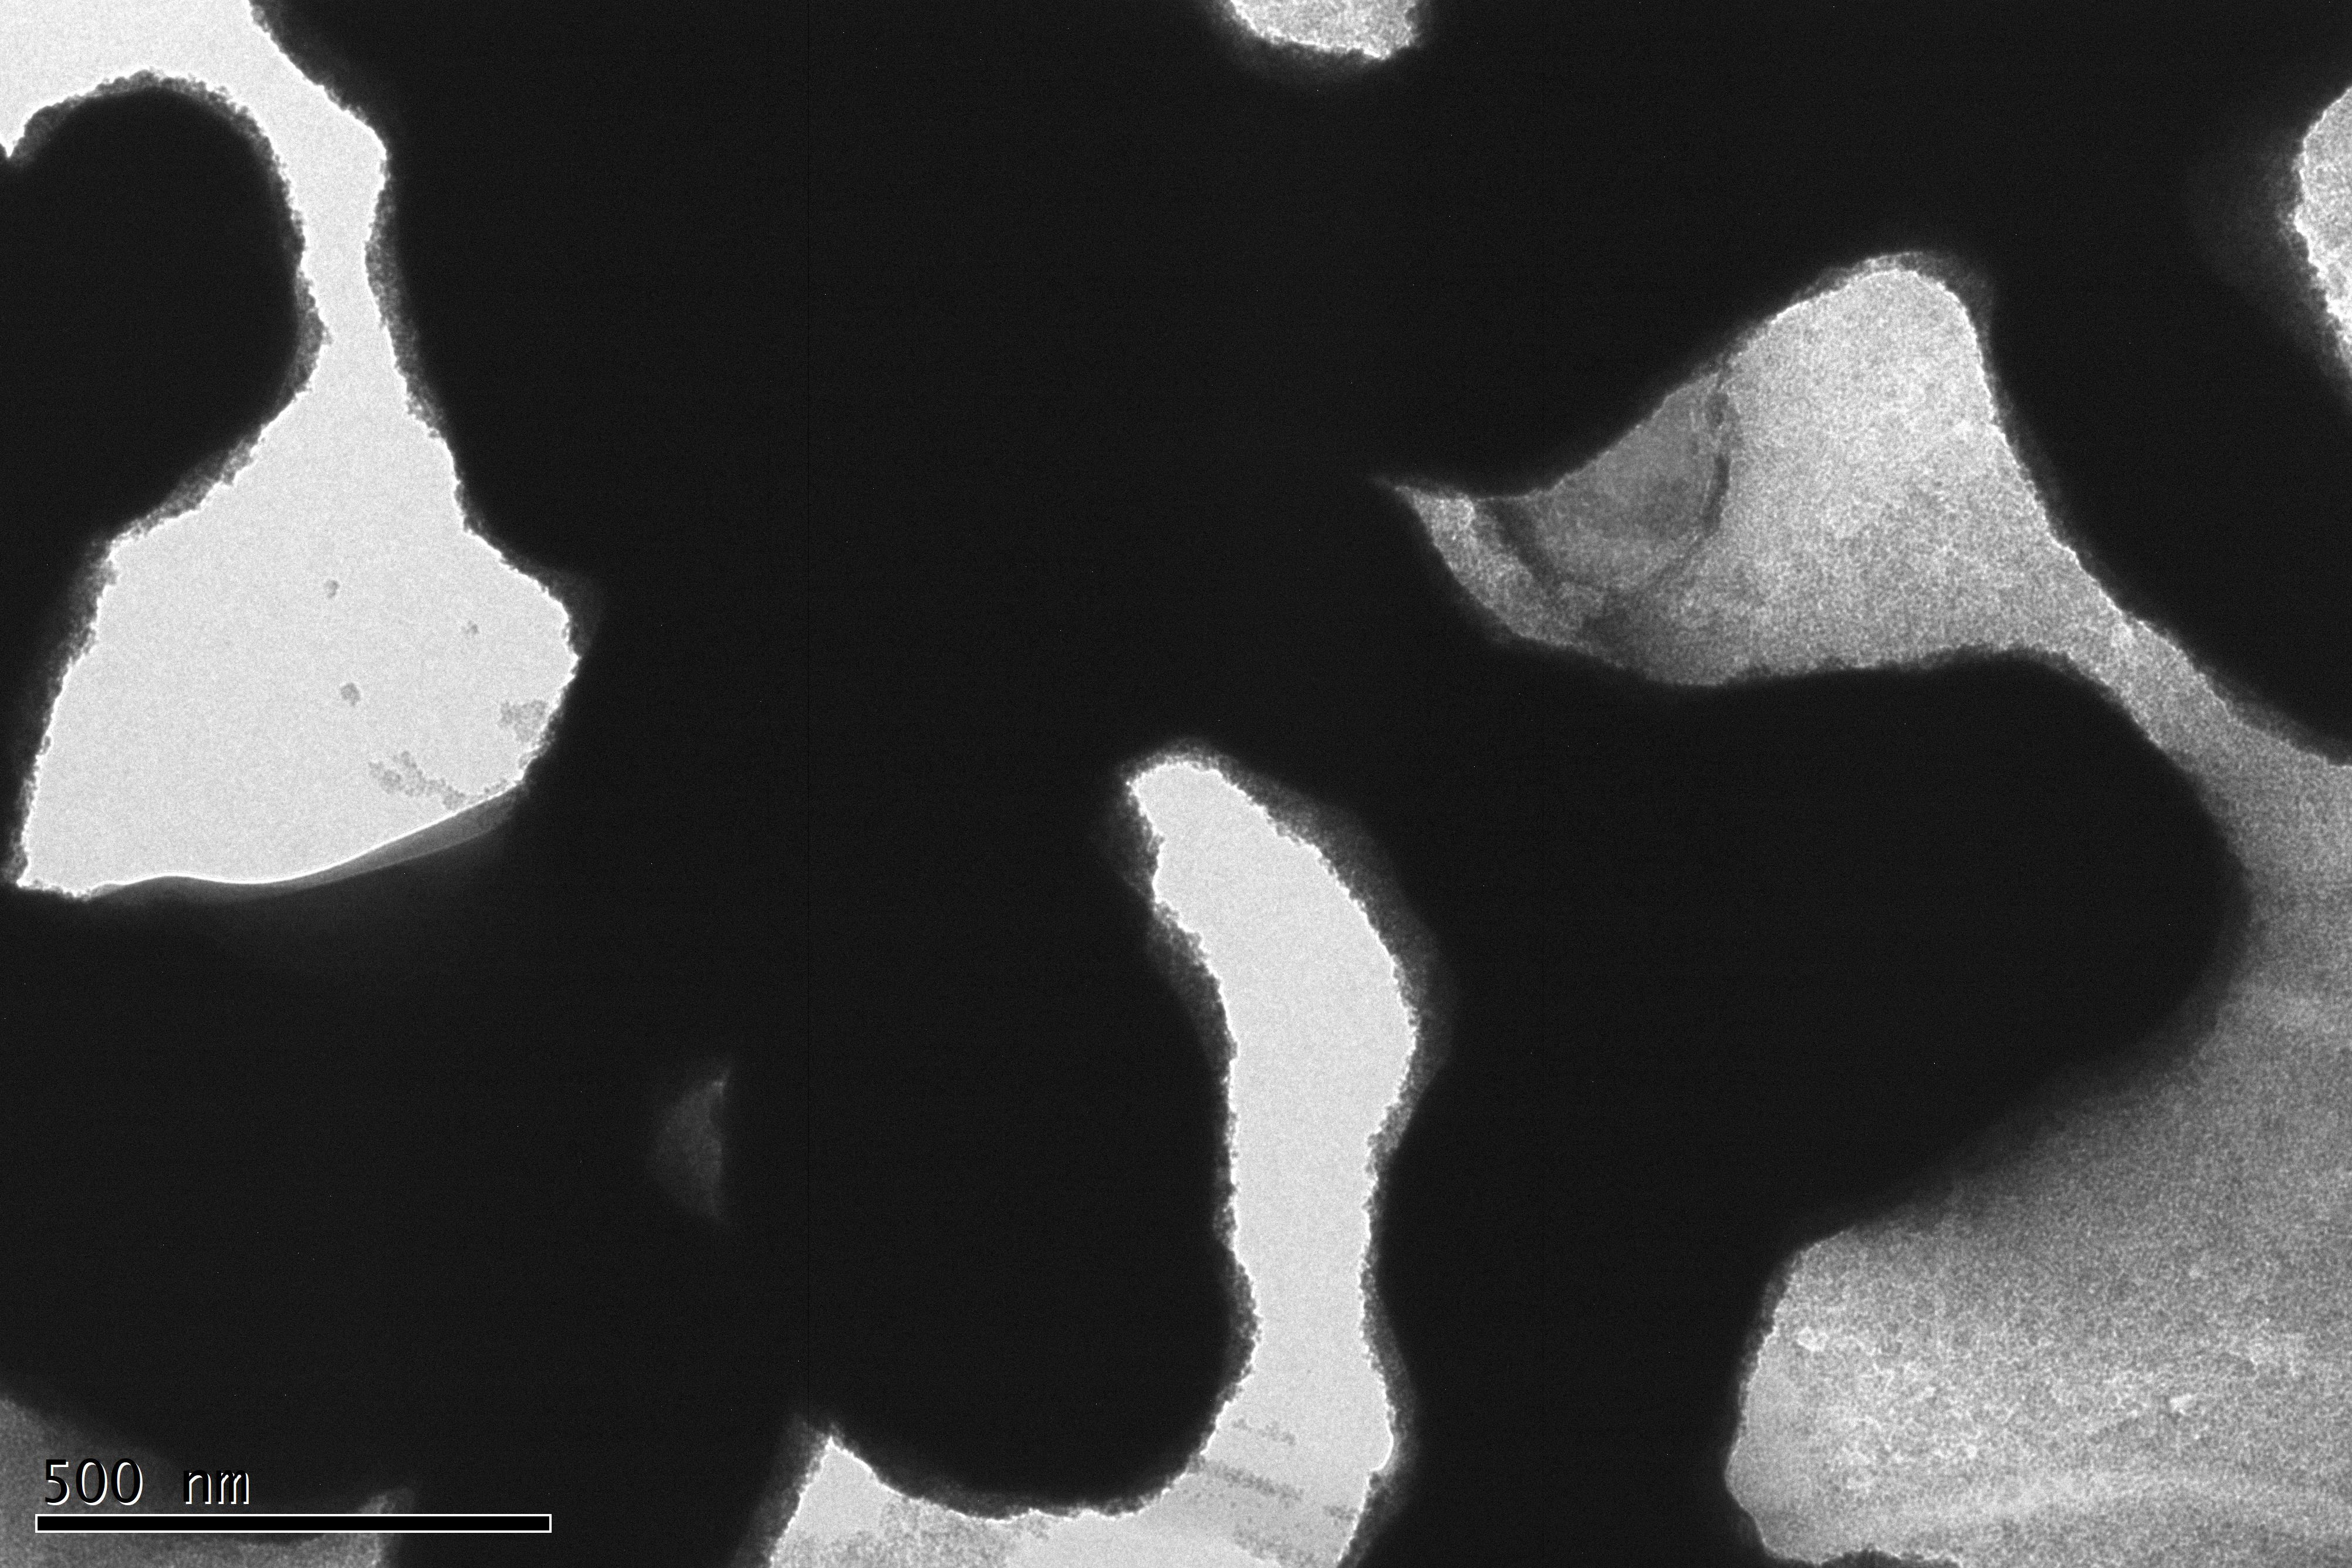
\includegraphics[width=0.33\linewidth]{Bilder/Gel-E-CdS_3}}
			\caption{TEM-Aufnahmen der Gele nach der thermischen Zersetzung von \ch{Cd[DDTC]2} zu CdS.}
			\label{fig:Gel-E-CdS}
		\end{figure}
	
		\begin{figure}[H]
			\centering
			\includegraphics[width=0.6\textwidth]{Bilder/Foto-CdS} 	
			\caption{Das Gel nach der Reaktion von \ch{Cd[DDTC]2}. Die typische Gelbfärbung von CdS ist deutlich zu erkennen.}
			\label{fig:Foto-CdS}
		\end{figure}
		
		Das Absorptionsspektrum, des mit \ch{Cd[DDTC]2} behandelten Gels, das in \cref{fig:UV-Gel-E-CdS} dargestellt ist, zeigt eine Bandkante bei \SI{440}{\nano\meter}, was einer Bandlücke von 2,82~eV entspricht. 
		Dieses Absorptionsmaximum ist energetisch deutlich höher als die Bandlücke des CdS als Bulk. 
		Da die CdS-Partikel jedoch, wie auf den TEM-Aufnahmen zu erkennen ist, sehr klein sind ($<$\SI{5}{\nano\meter}), kann dies durch den Größenquantisierungseffekt erklärt werden.
		
		\begin{figure}[H]
			\centering
			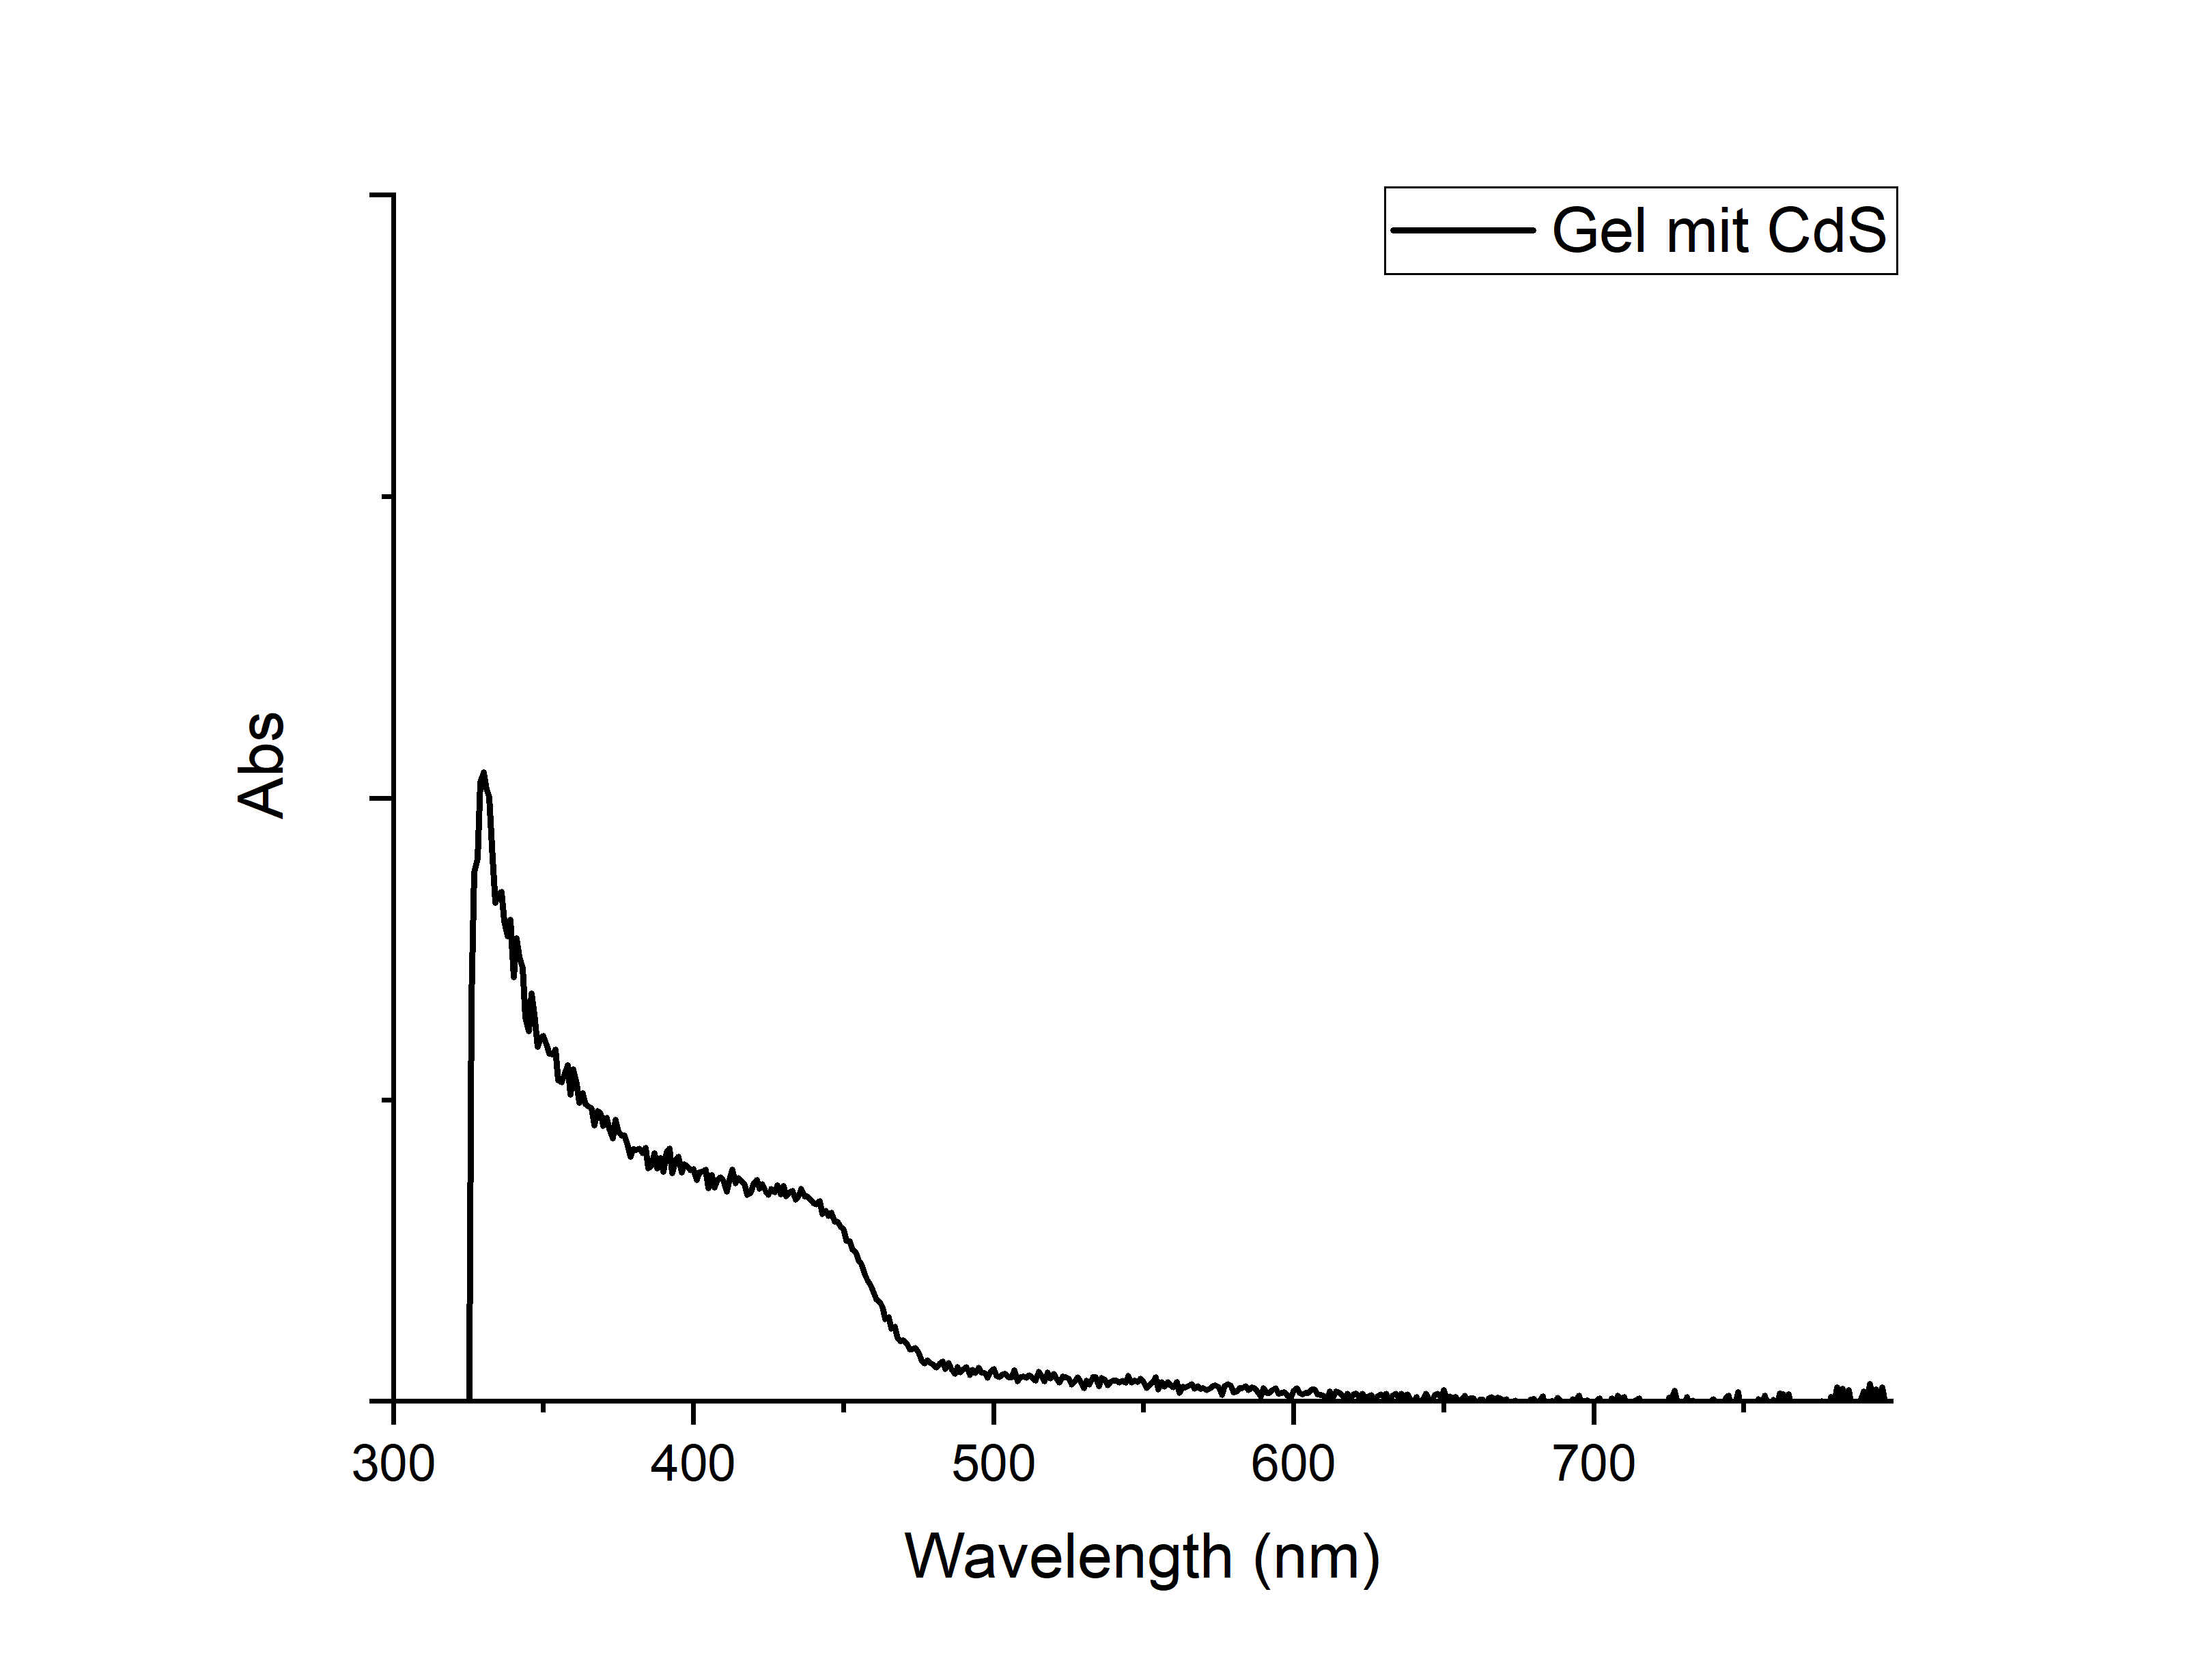
\includegraphics[width=0.6\textwidth]{Bilder/UV-Gel-E-CdS} 	
			\caption{Absorptionsspektrum des Gels, das mit \ch{Cd[DDTC]2} behandelt wurde.}
			\label{fig:UV-Gel-E-CdS}
		\end{figure}
	
		Während bei der Probe mit \ch{Cd[DDTC]2} eine fast komplette Schale um das Gel beobachtet werden konnte, waren die Ergebnisse bei der Behandlung mit \ch{Zn[DDTC]2} deutlich anders.
		So lassen sich bei den TEM-Aufnahmen, die in \cref{fig:Gel-E-ZnS} gezeigt sind, keine Partikel am Gel erkennen und auch das Absorptionsspektrum zeigte nichts, wie \cref{fig:UV-Gel-E-ZnS} zeigt.
		Da das Gel selbst aber schon ein dunkler Körper ist, hätte im sichtbaren Bereich eigentlich eine Absorption zu messen sein müssen.
		Das deutet darauf hin, dass die Probe nicht richtig getroffen wurde.
		Auch nach mehrmaligen Versuchen gelang dies, aufgrund der geringen Probenmenge, nicht. 
		
		\begin{figure}[H]
			\centering
			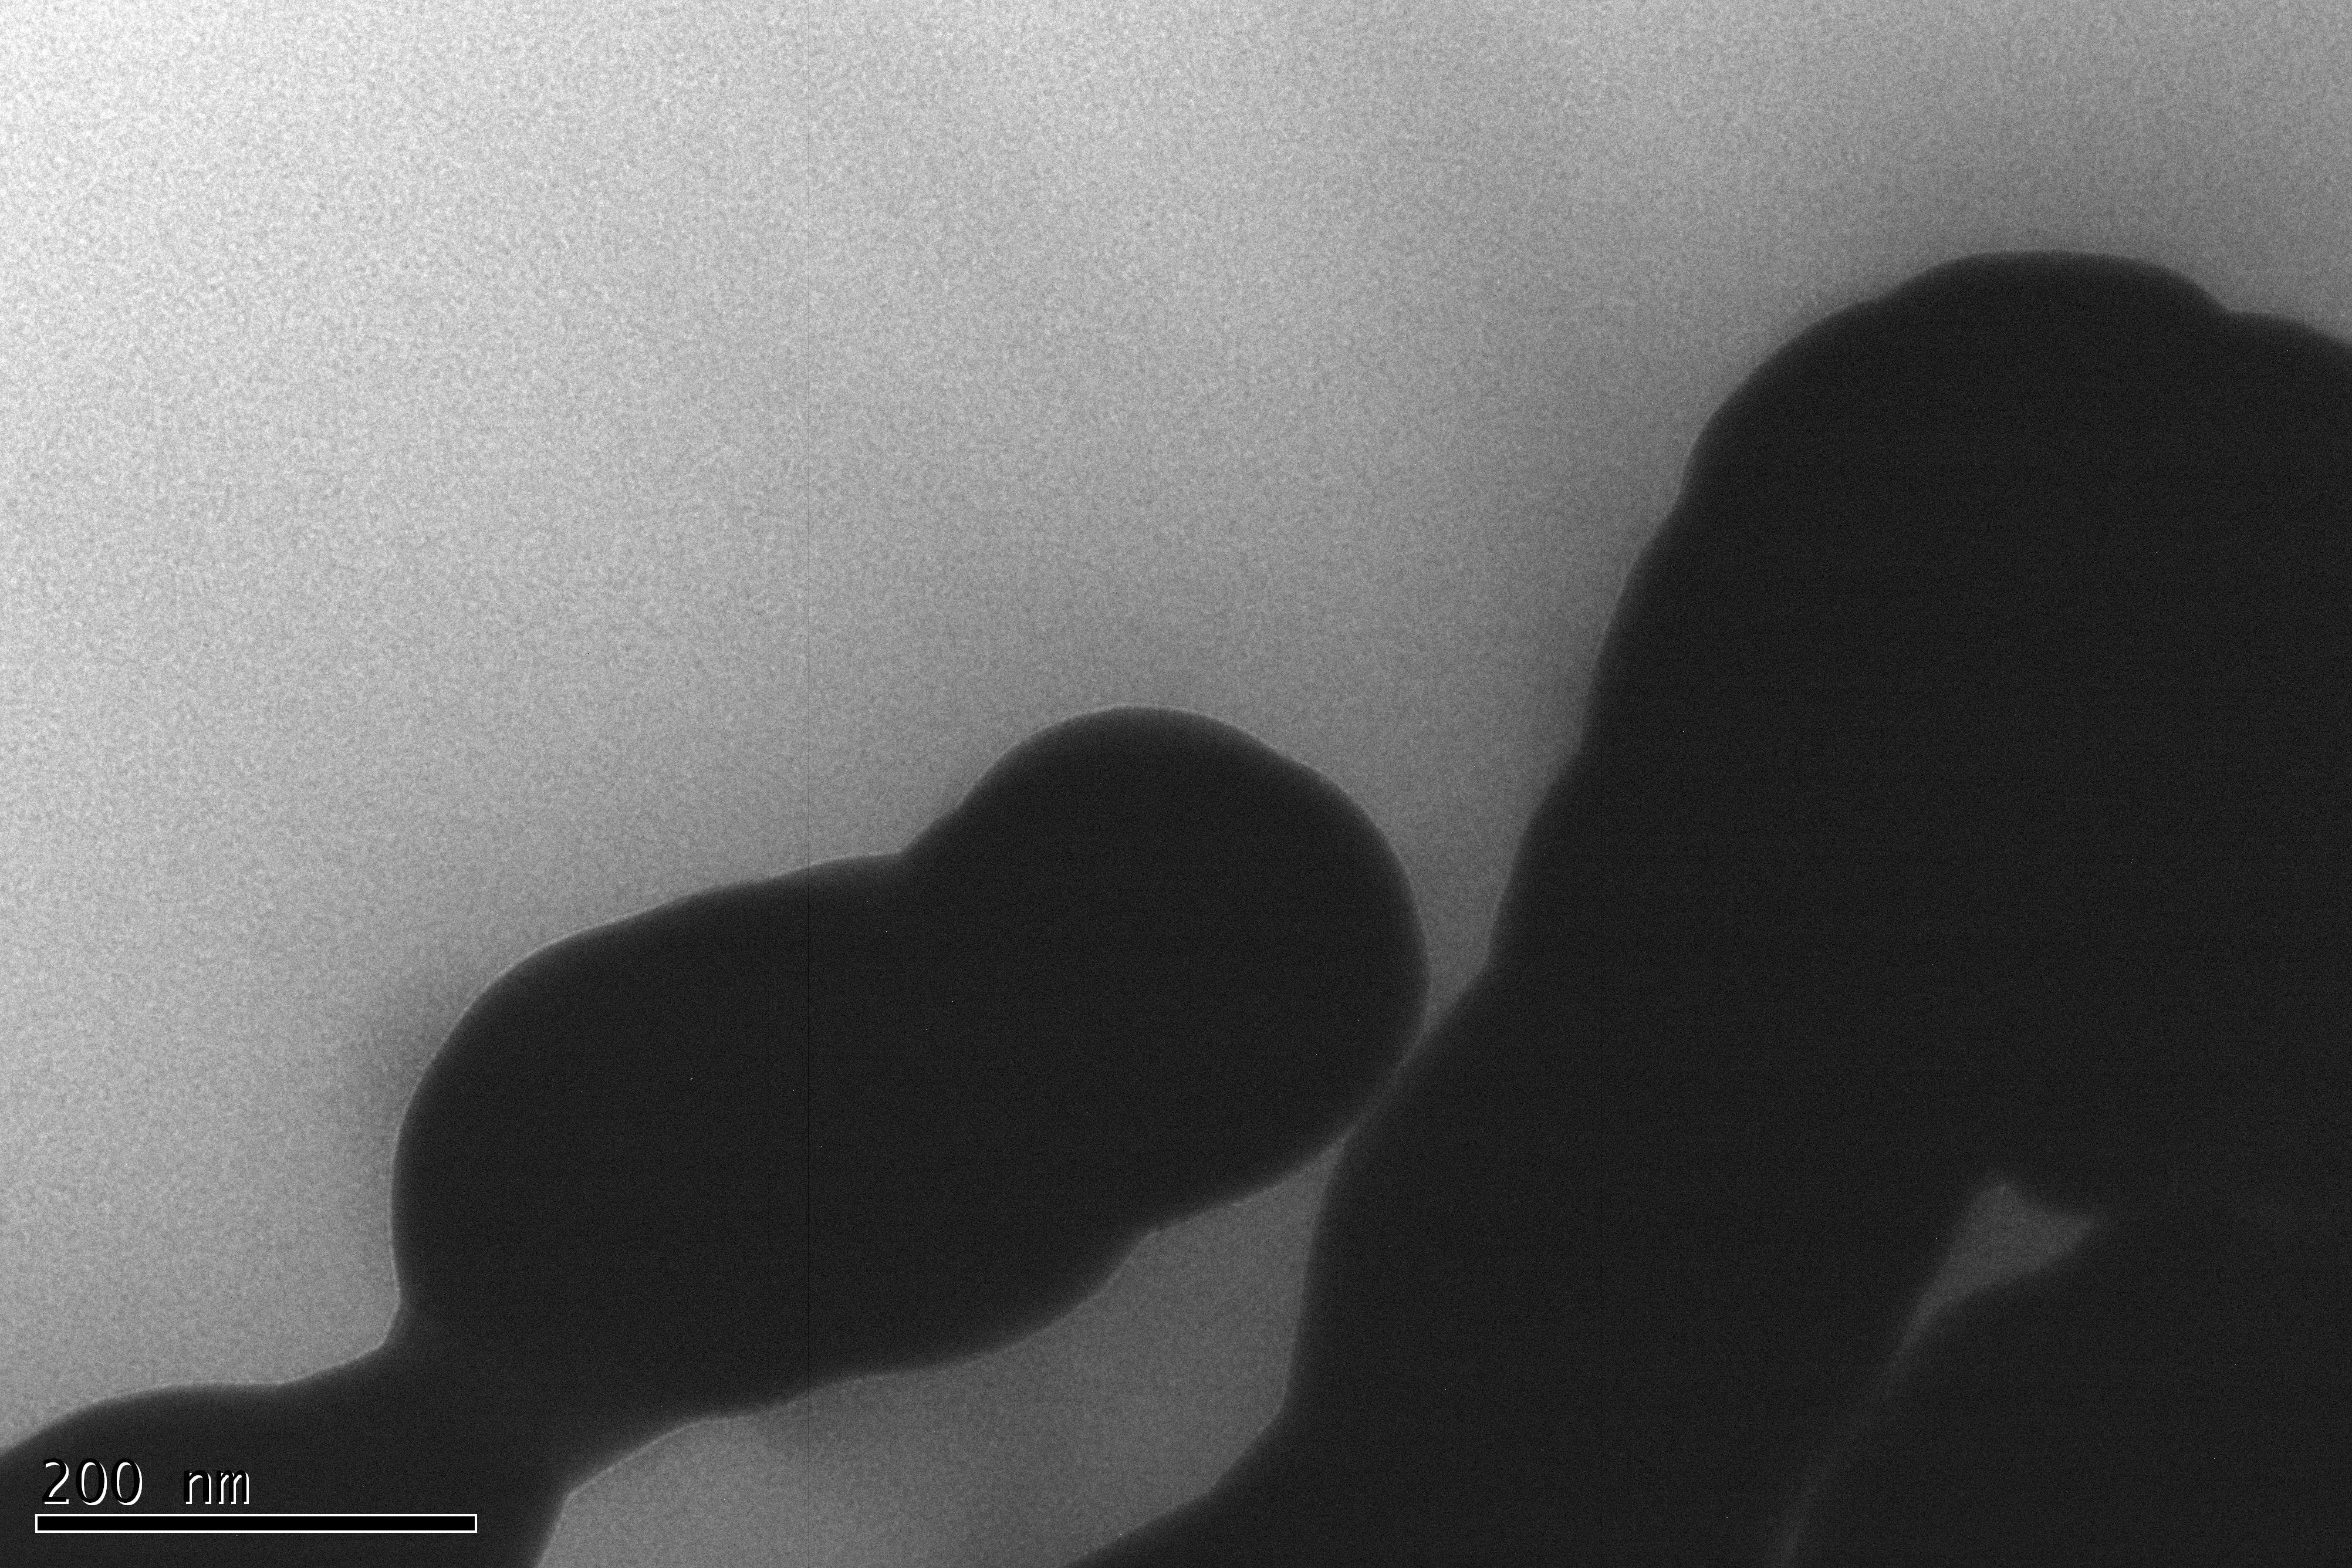
\includegraphics[width=0.6\textwidth]{Bilder/Gel-E-ZnS} 	
			\caption{TEM-Aufnahmen der Gele nach der Behandlung mit \ch{Zn[DDTC]2}.}
			\label{fig:Gel-E-ZnS}
		\end{figure}
		
		\begin{figure}[H]
			\centering
			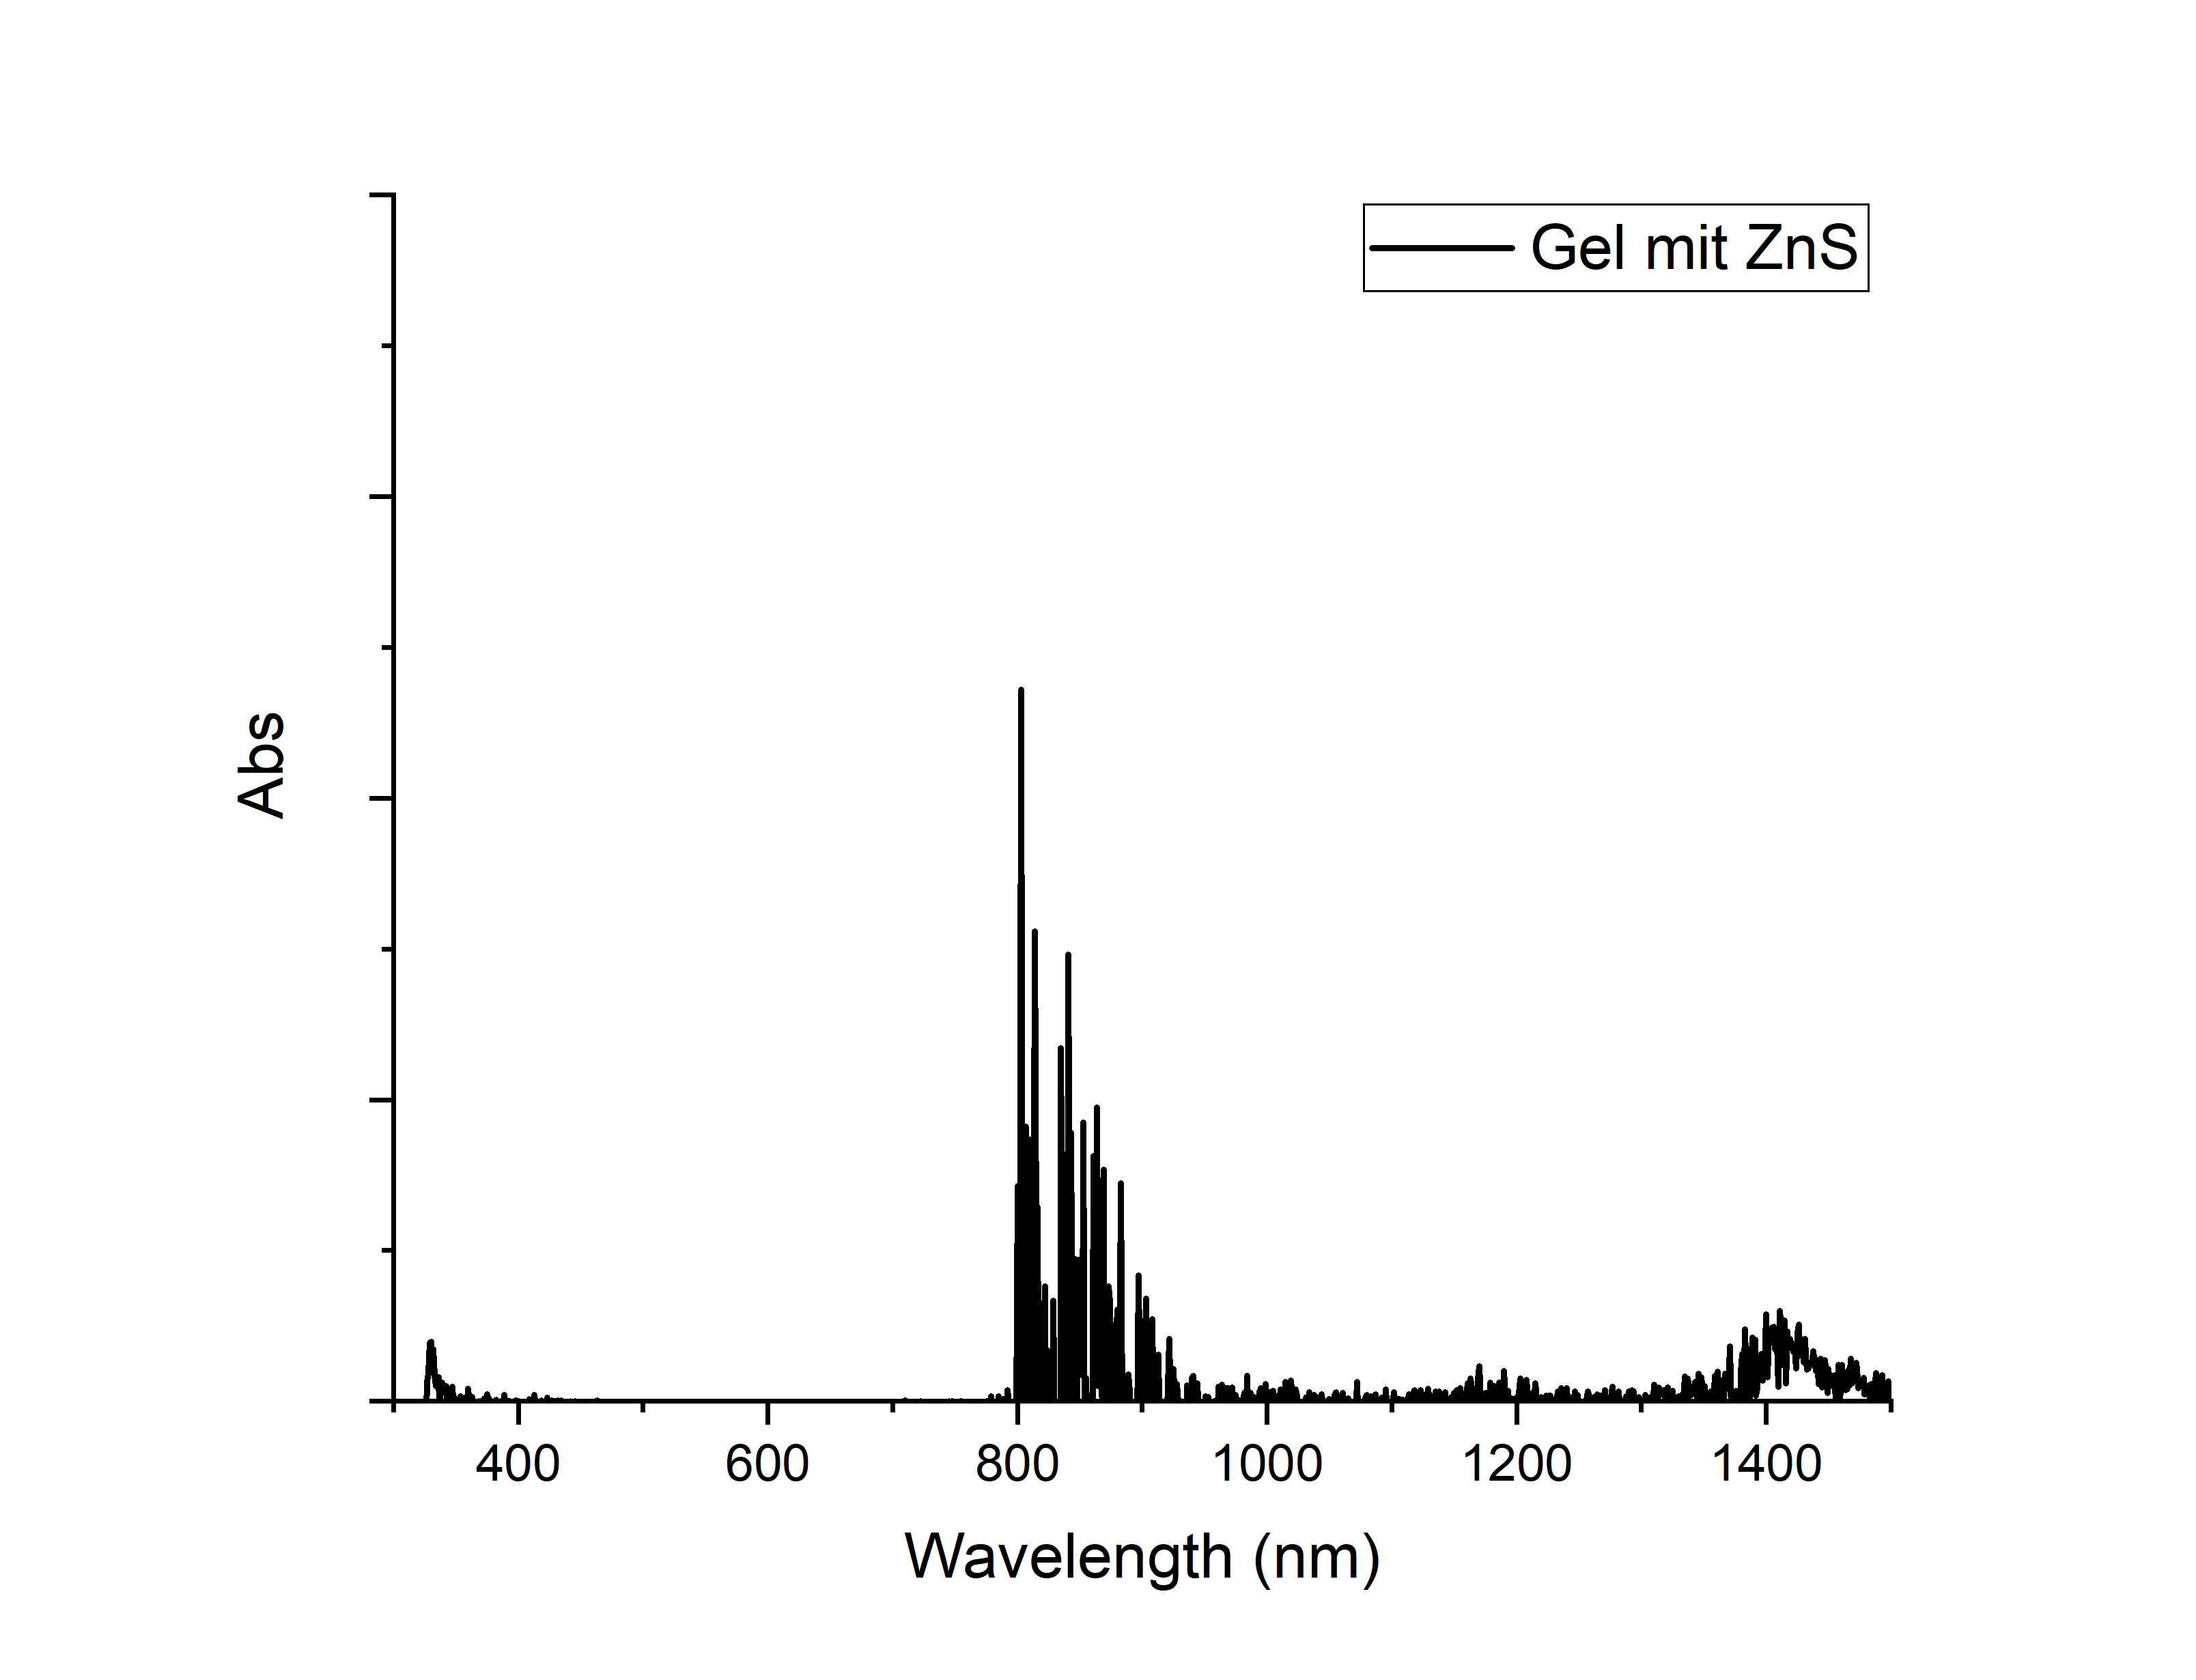
\includegraphics[width=0.6\textwidth]{Bilder/UV-Gel-E-ZnS} 	
			\caption{Absorptionsspektrum des Gels, das mit \ch{Zn[DDTC]2} behandelt wurde.}
			\label{fig:UV-Gel-E-ZnS}
		\end{figure}
	
	\subsubsection{Zusatz von Chloridionen}
	
		Da, wie schon oben gezeigt, das Nukleationsverhalten durch Anwesenheit von Chlorid beeinflusst werden kann, wurde dies auch bei Anwesenheit der Gele untersucht.
		Dabei zeigten sich deutliche Unterschiede zwischen \ch{Cd[DDTC]2} und \ch{Zn[DDTC]2}.
		
		Bei den Proben, die mit \ch{Cd[DDTC]2} und \ch{CdCl2} behandelt wurden, verschlechterte sich das Ergebnis deutlich, wie in \cref{fig:Gel-E-CdCl} gezeigt ist.
		Die Bilder zeigen, dass das gebildete CdS nicht am Gel anliegt sondern sich überall befindet.
		Durch die Zugabe von \ch{CdCl2} scheint sich das Nukleationsverhalten, wie auch schon bei den Versuchen ohne das Gel erklärt, so zu ändern, dass die Partikel abgetrennt vom Gel gebildet werden, was das Verhindern des Anwachsens erklärt.  
		
		\begin{figure}[H]
			\centering
			\subfloat[\label{fig:Gel-E-CdCl-1-1}]{%
				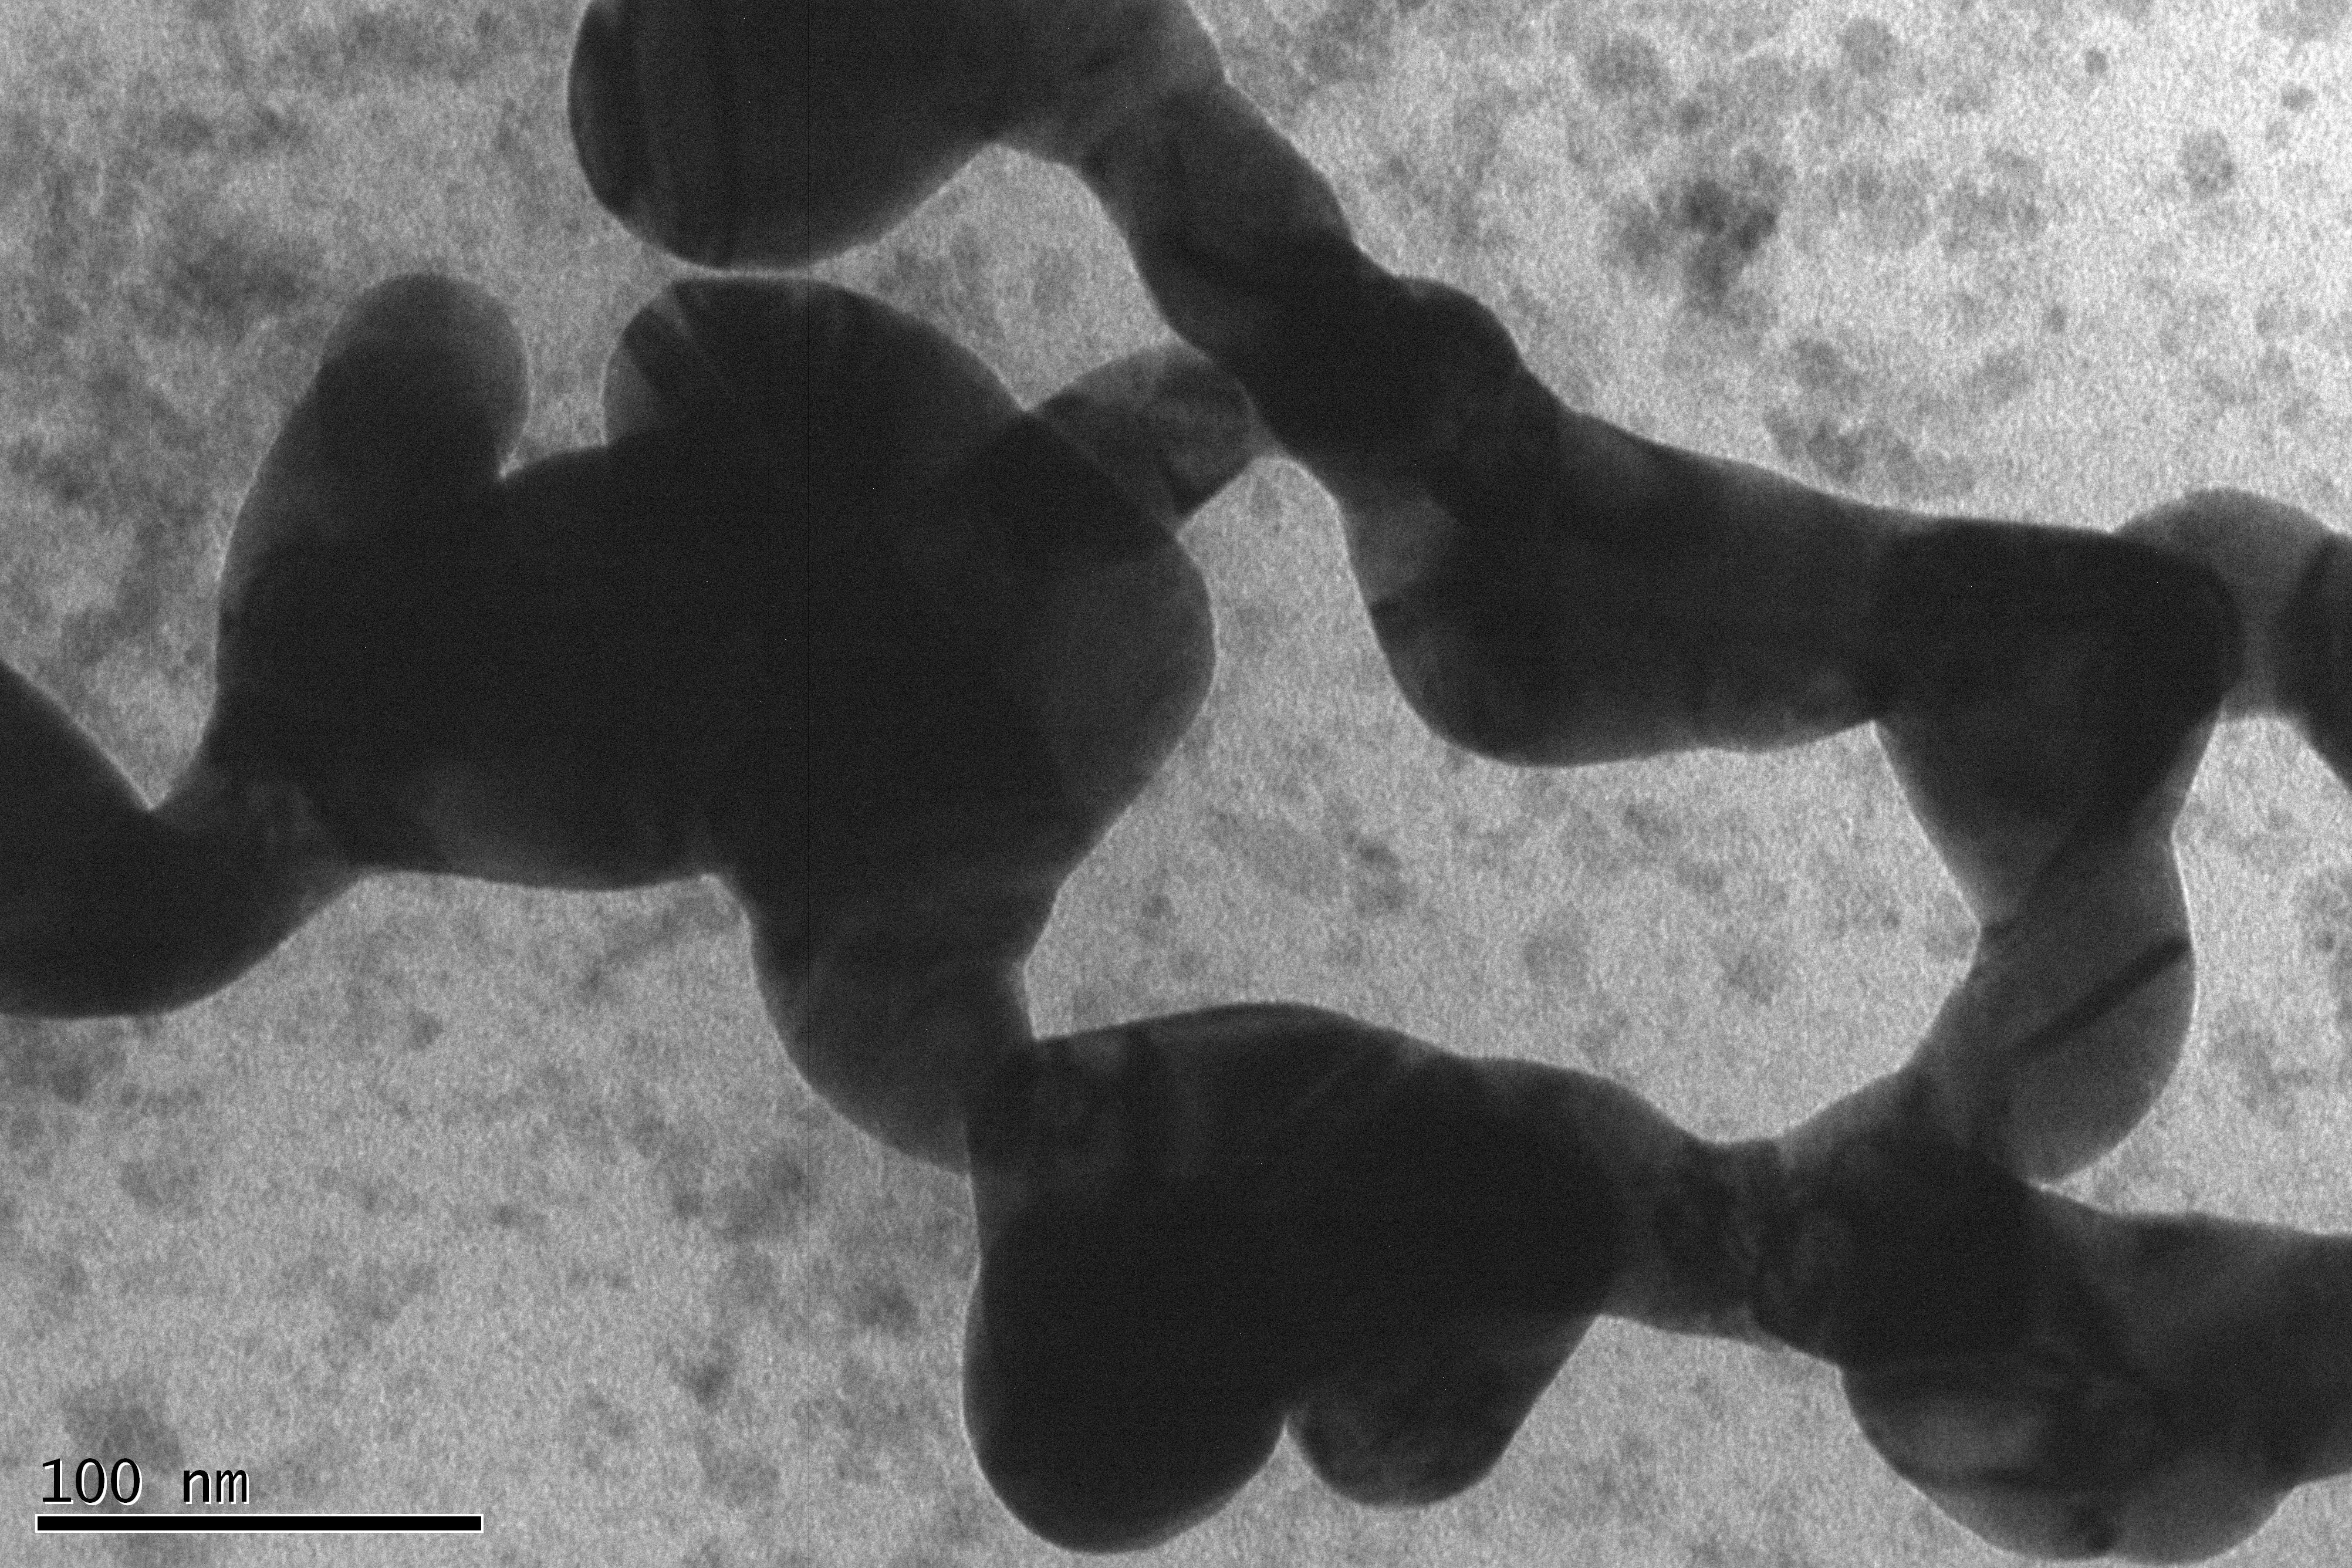
\includegraphics[width=0.33\linewidth]{Bilder/Gel-E-CdCl-1-1}}
			\subfloat[\label{fig:Gel-E-CdCl-1-4}]{%
				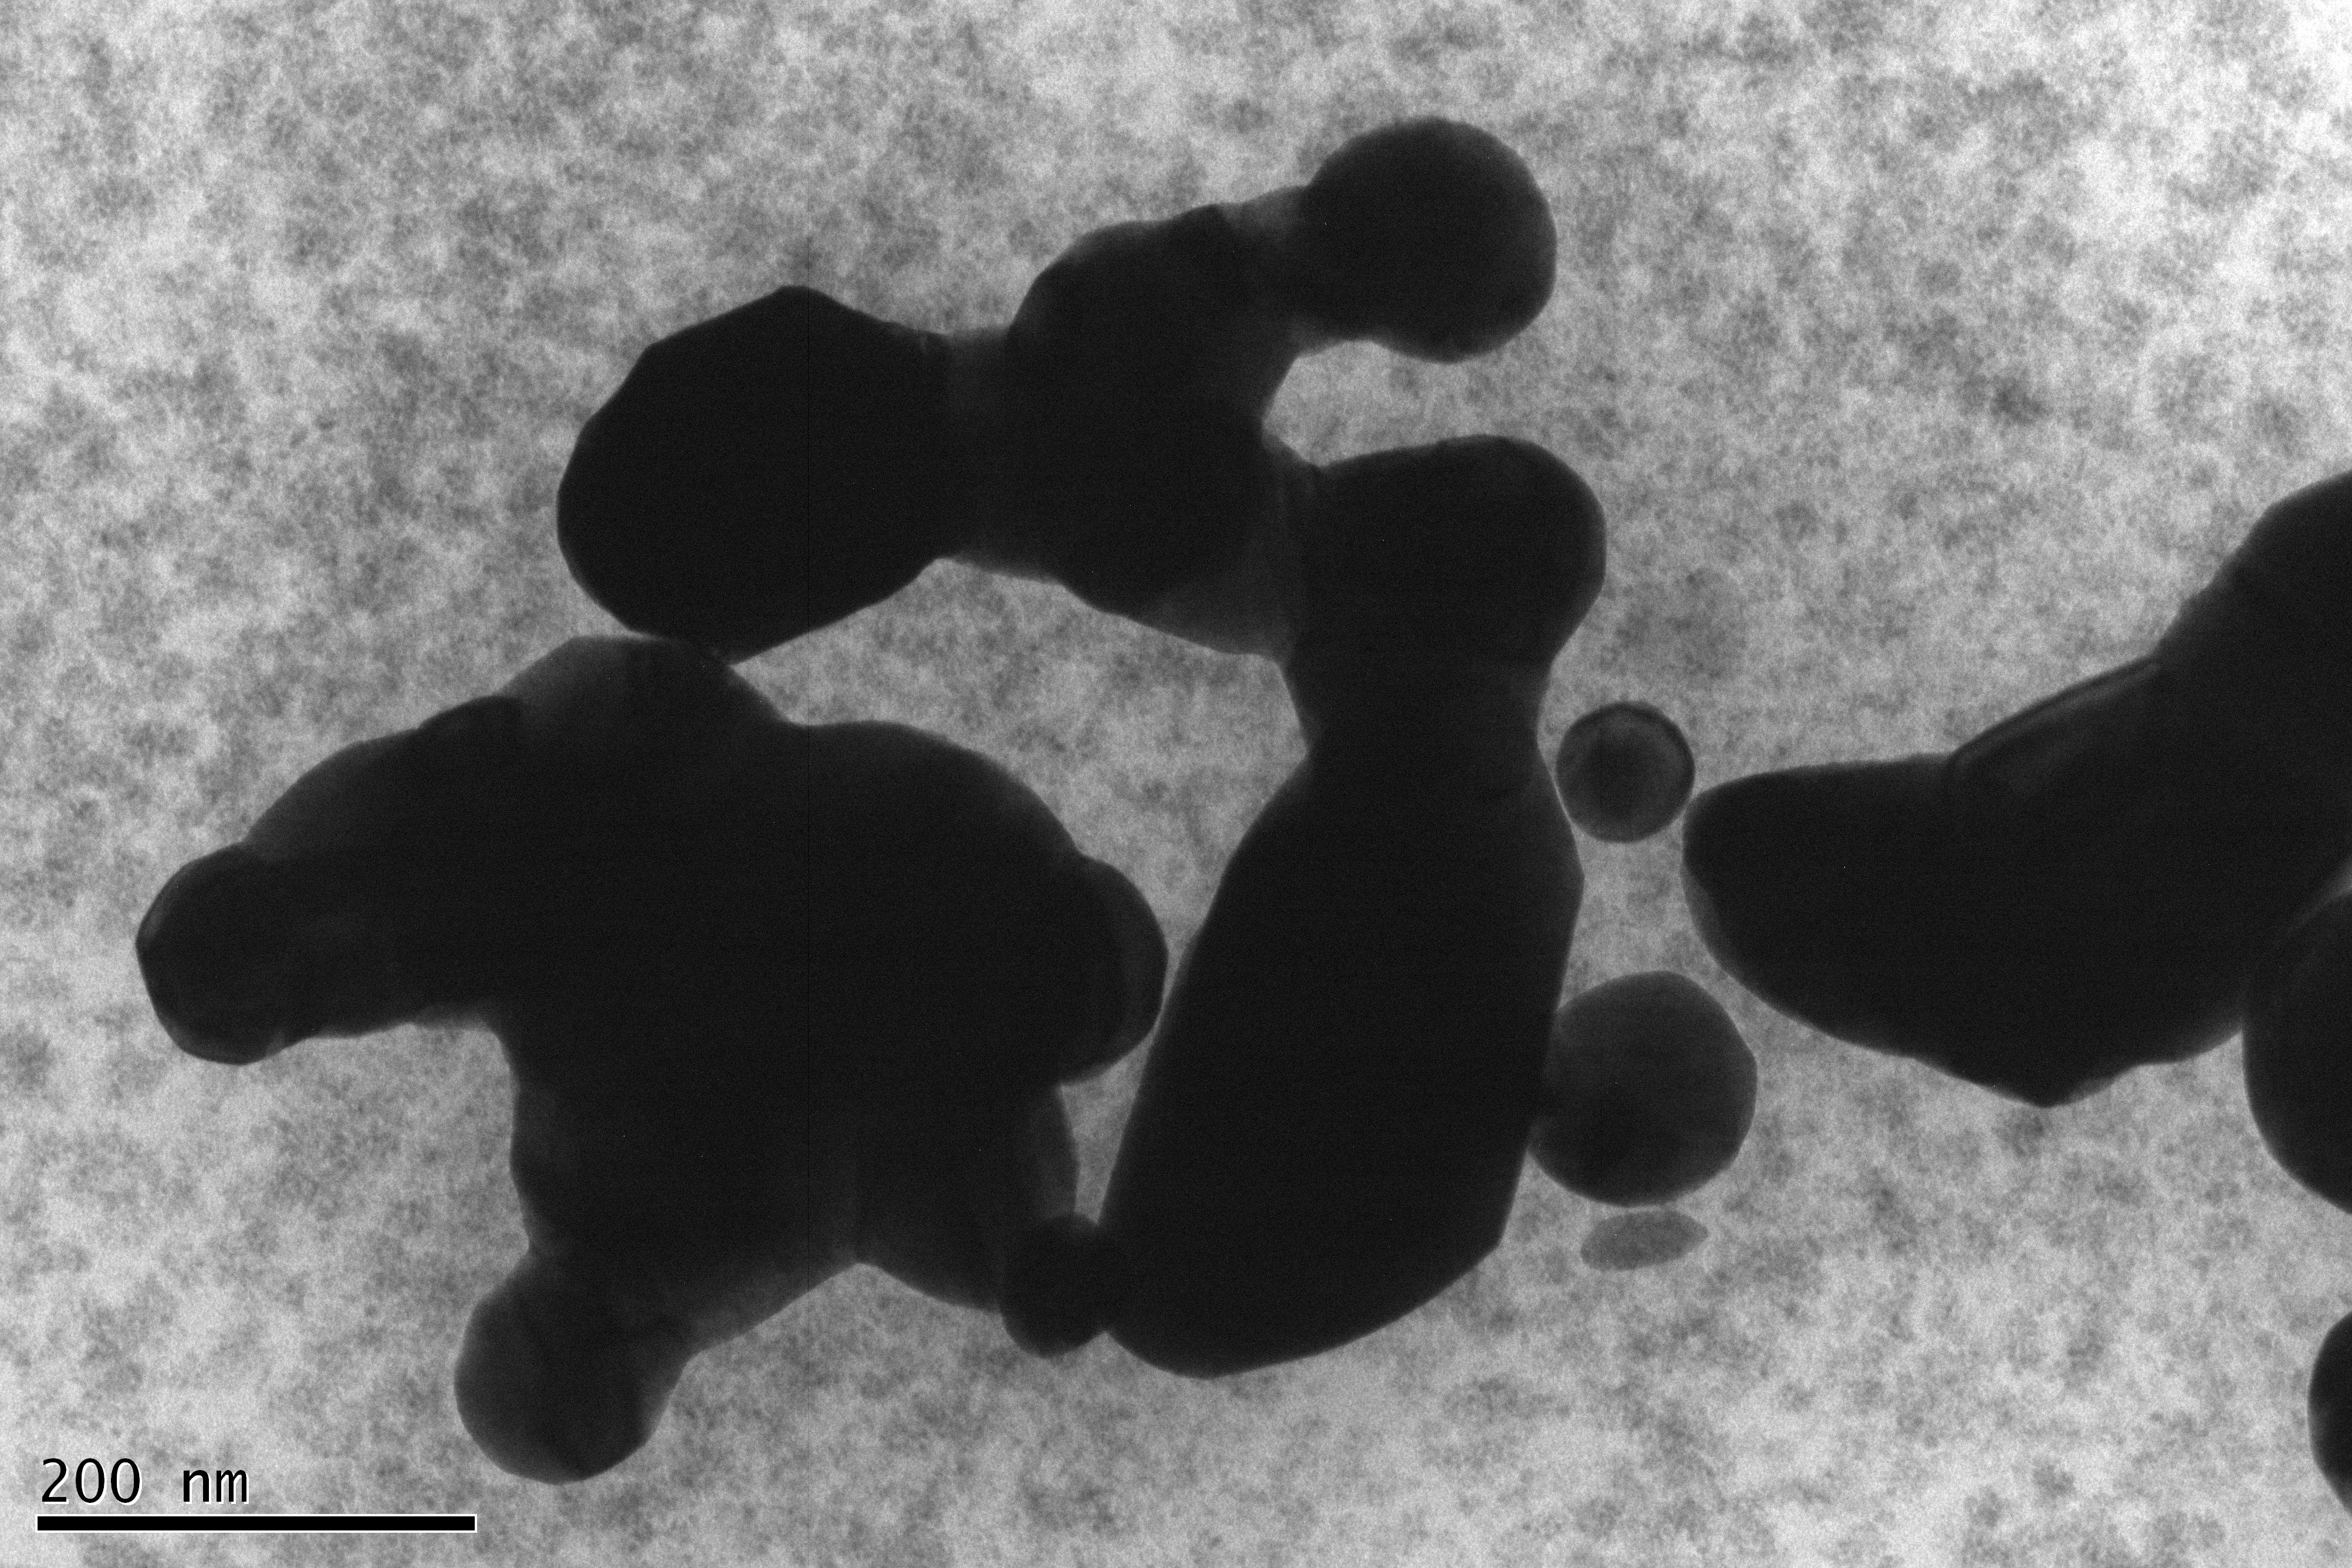
\includegraphics[width=0.33\linewidth]{Bilder/Gel-E-CdCl-1-4}}
			\subfloat[\label{fig:Gel-E-CdCl-1-10}]{%
				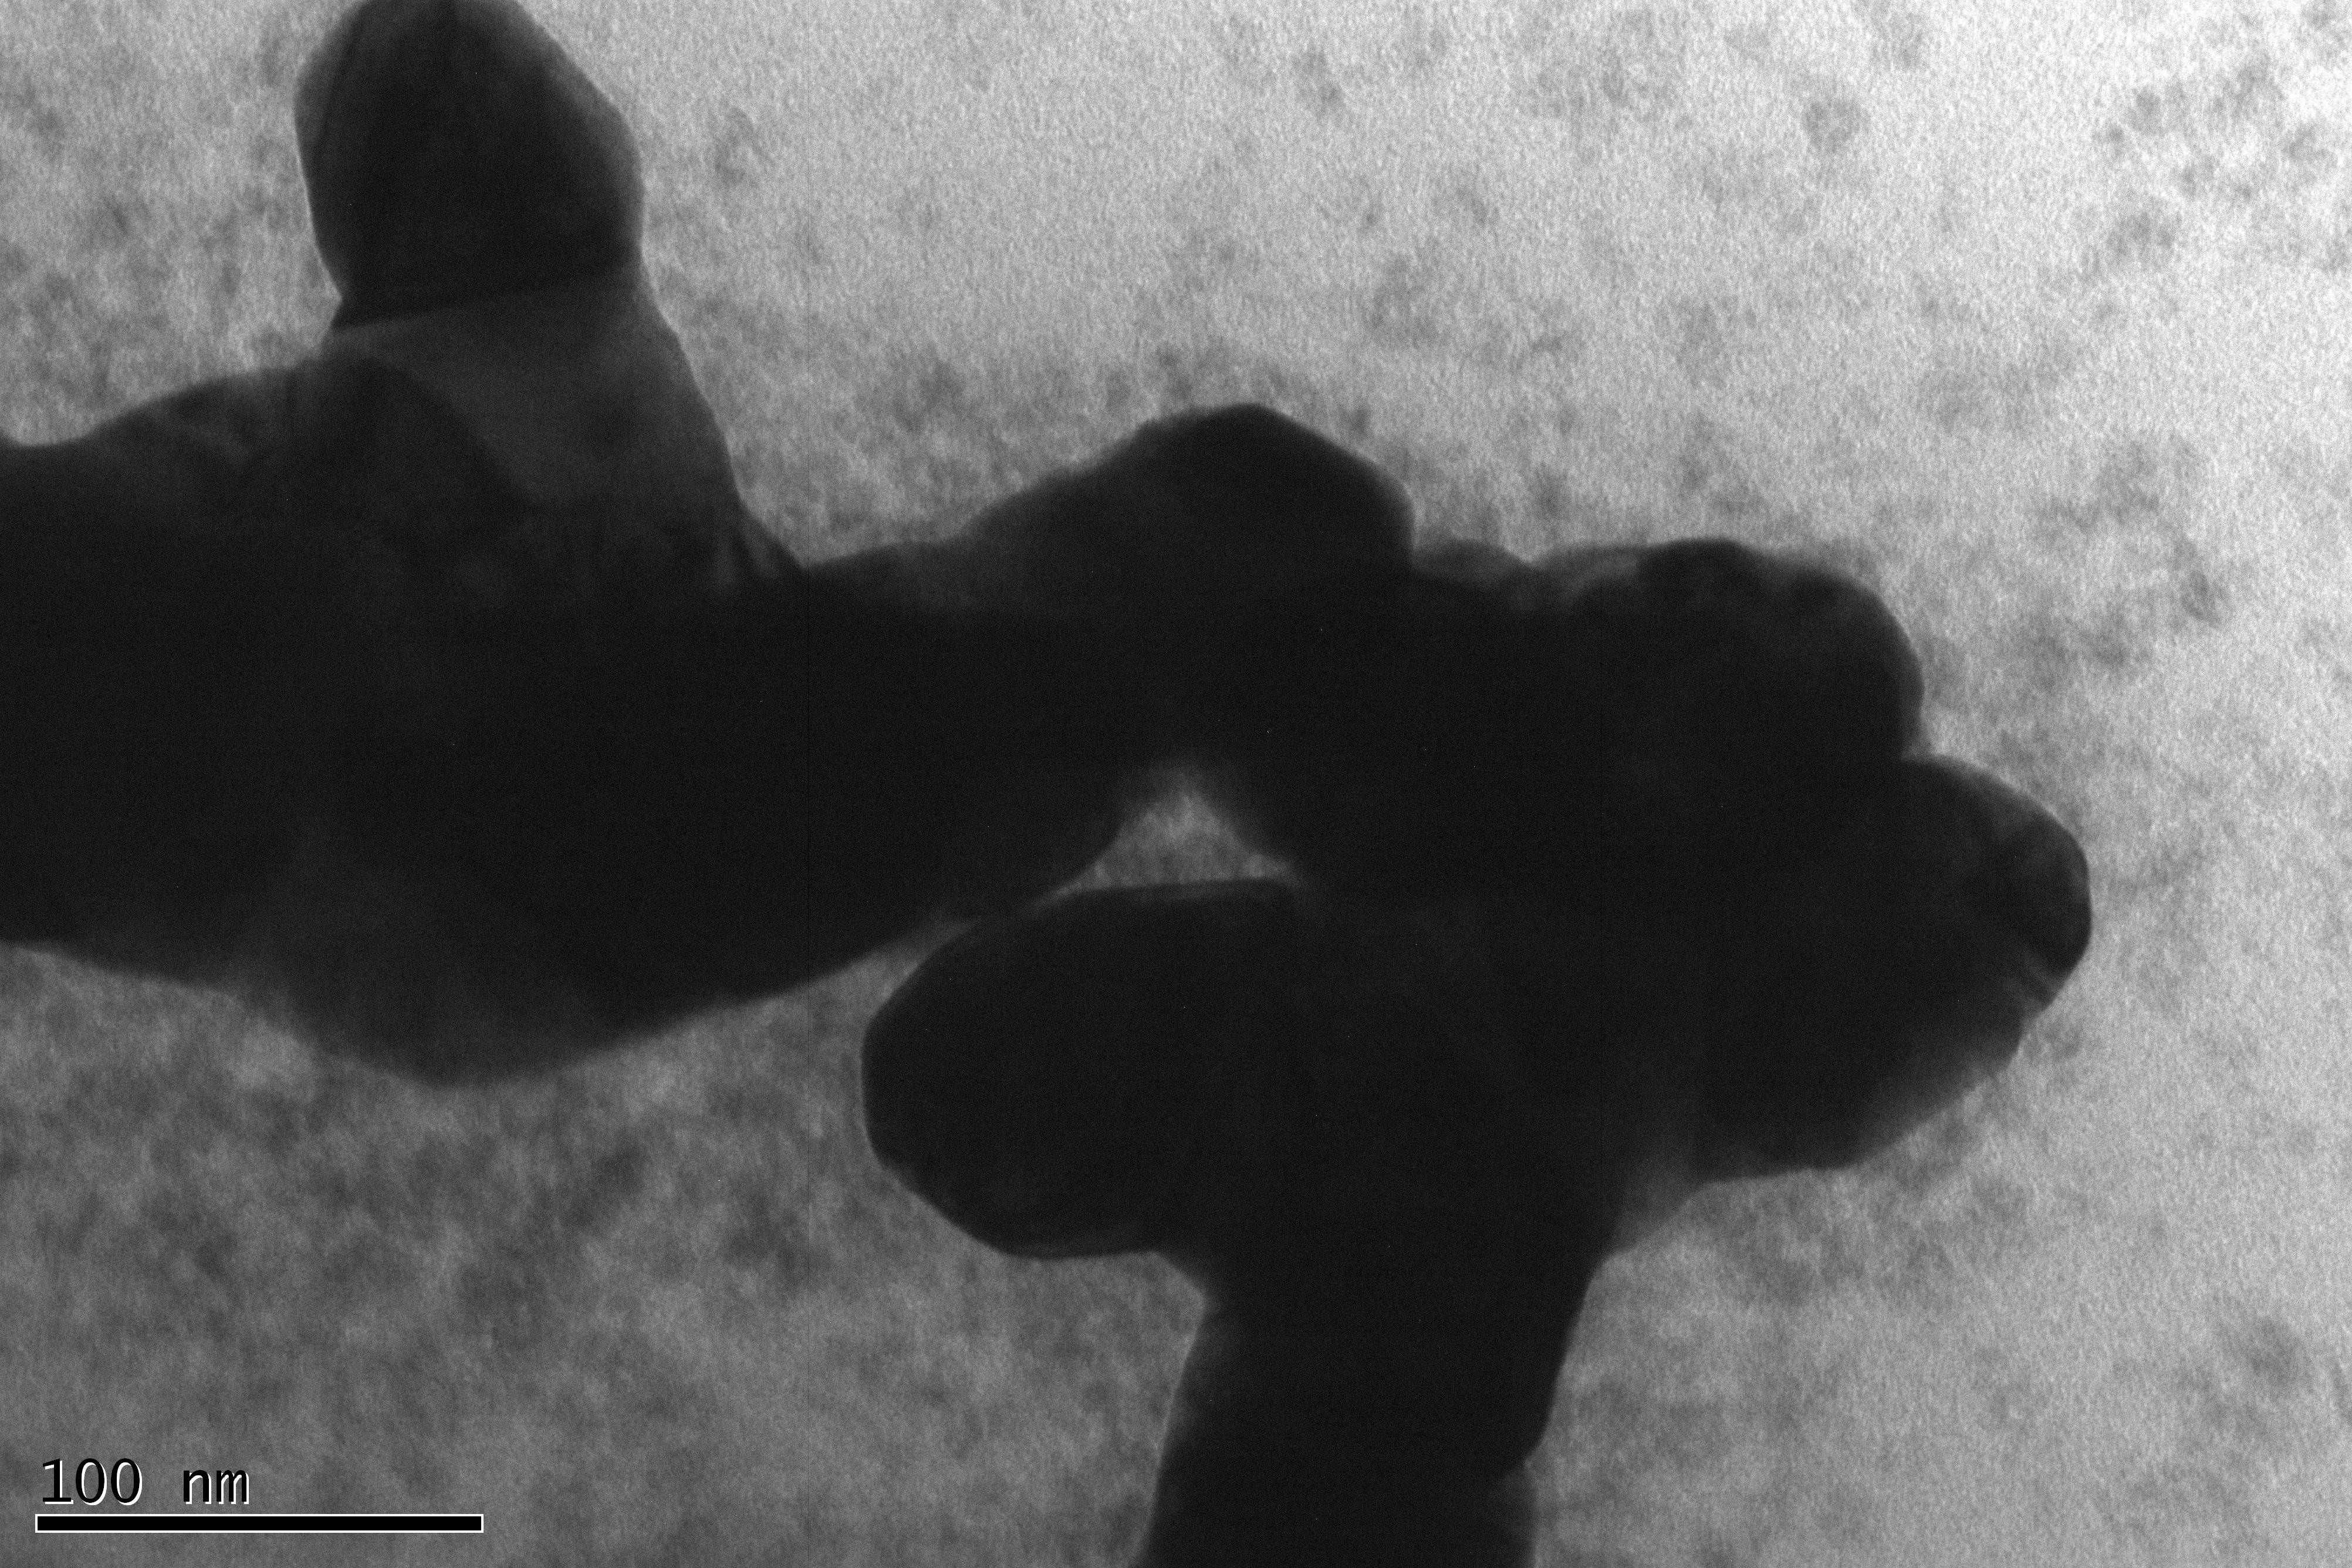
\includegraphics[width=0.33\linewidth]{Bilder/Gel-E-CdCl-1-10}}
			\caption{TEM-Aufnahmen der Gele, die mit \ch{Cd[DDTC]2} und \ch{CdCl2} im Verhältnis \emph{(a)}: 1:1; \emph{(b)}: 1:4; \emph{(c)}: 1:10 \ch{Cd[DDTC]2} zu \ch{CdCl2} behandelt wurden.}
			\label{fig:Gel-E-CdCl}
		\end{figure}
		
		Bei den Proben die mit \ch{Zn[DDTC]2} und \ch{ZnCl2} behandelt wurden ließ sich etwas anderes beobachten.
		Während hier keine Partikelbildung bei reinem \ch{Zn[DDTC]2} zu erkennen war, konnte dies durch Zugabe vom \ch{ZnCl2} verändert werden.
		Bei den Proben, die im Verhältnis 1:1 (\cref{fig:Gel-E-ZnCl-1-1})und 1:10 (\cref{fig:Gel-E-ZnCl-1-10}) \ch{Zn[DDTC]2} zu \ch{ZnCl2} behandelt wurden, konnte an einigen Stellen die Ausbildung von einer dünnen Schicht an den Gelen beobachtet werden.
		Bei der Probe im 1:10 Verhältnis konnte dabei sogar eine komplette Hülle um einige Teile des Gels beobachtet werden, was besonders gut in \cref{fig:Gel-E-ZnCl-1-10_1} zu erkennen ist.
		
		\begin{figure}[H]
			\centering
			\subfloat[\label{fig:Gel-E-ZnCl-1-1_1}]{%
				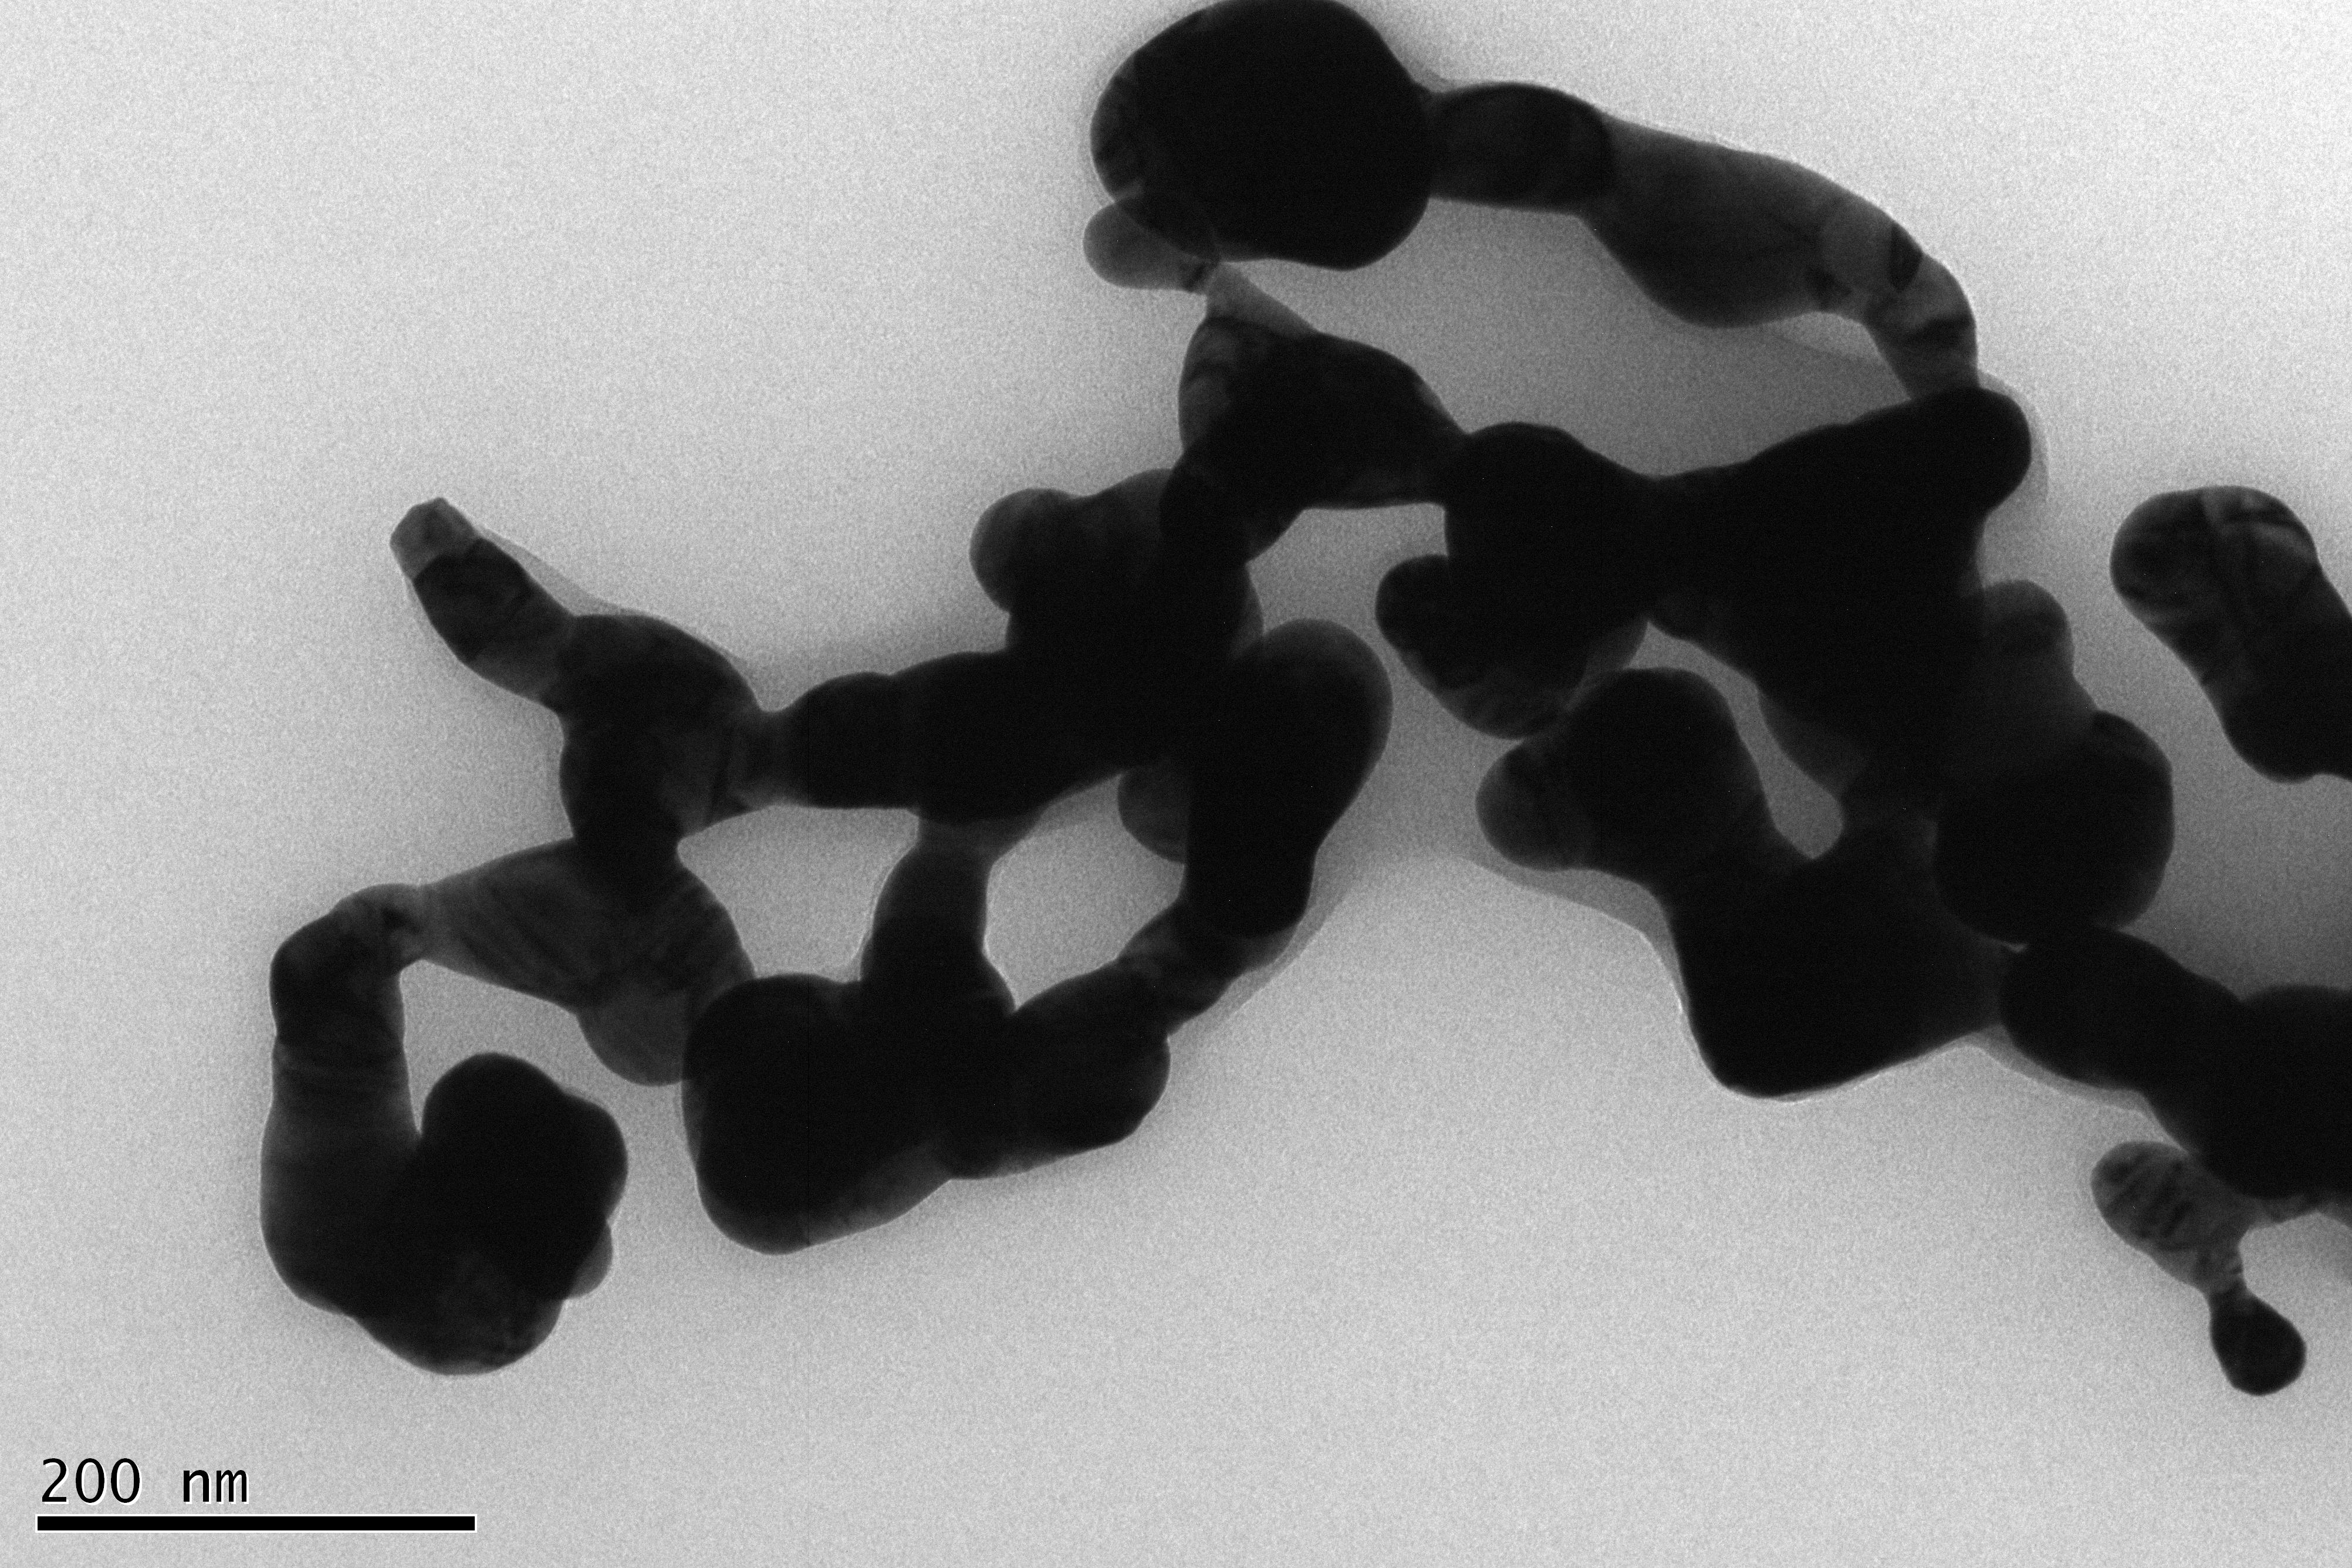
\includegraphics[width=0.33\linewidth]{Bilder/Gel-E-ZnCl-1-1_1}}
			\subfloat[\label{fig:Gel-E-ZnCl-1-1_2}]{%
				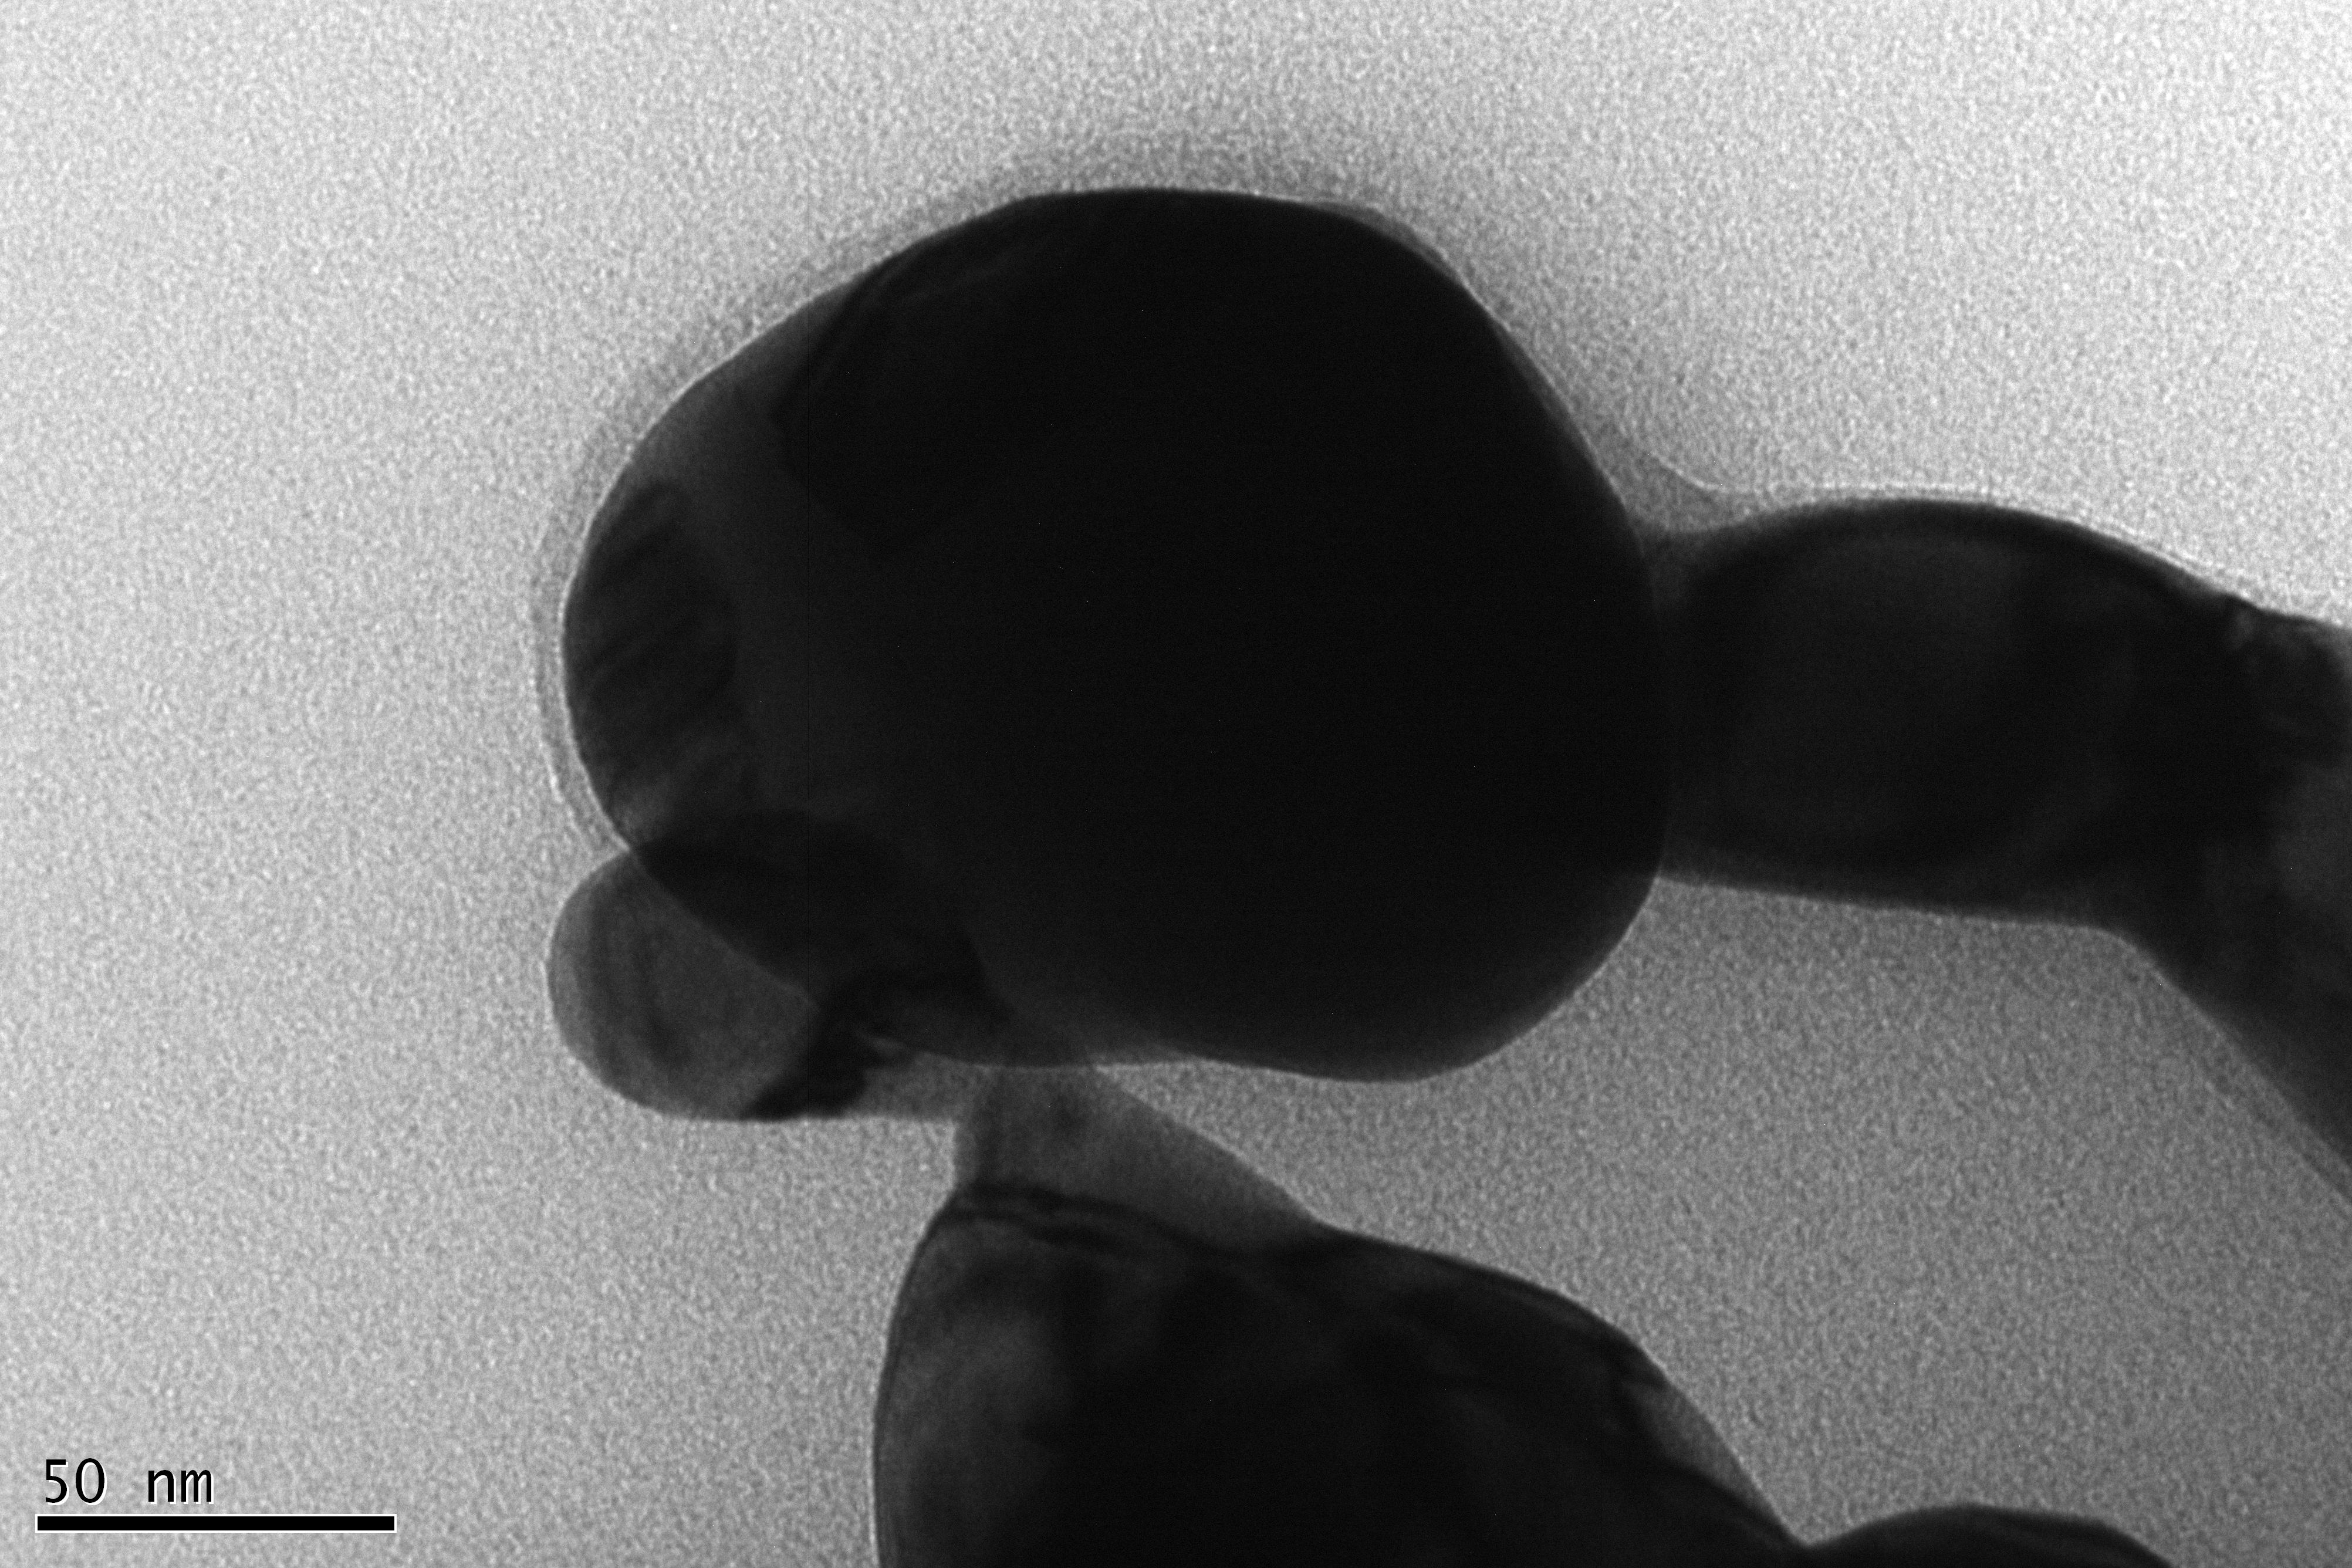
\includegraphics[width=0.33\linewidth]{Bilder/Gel-E-ZnCl-1-1_2}}
			\subfloat[\label{fig:Gel-E-ZnCl-1-1_3}]{%
				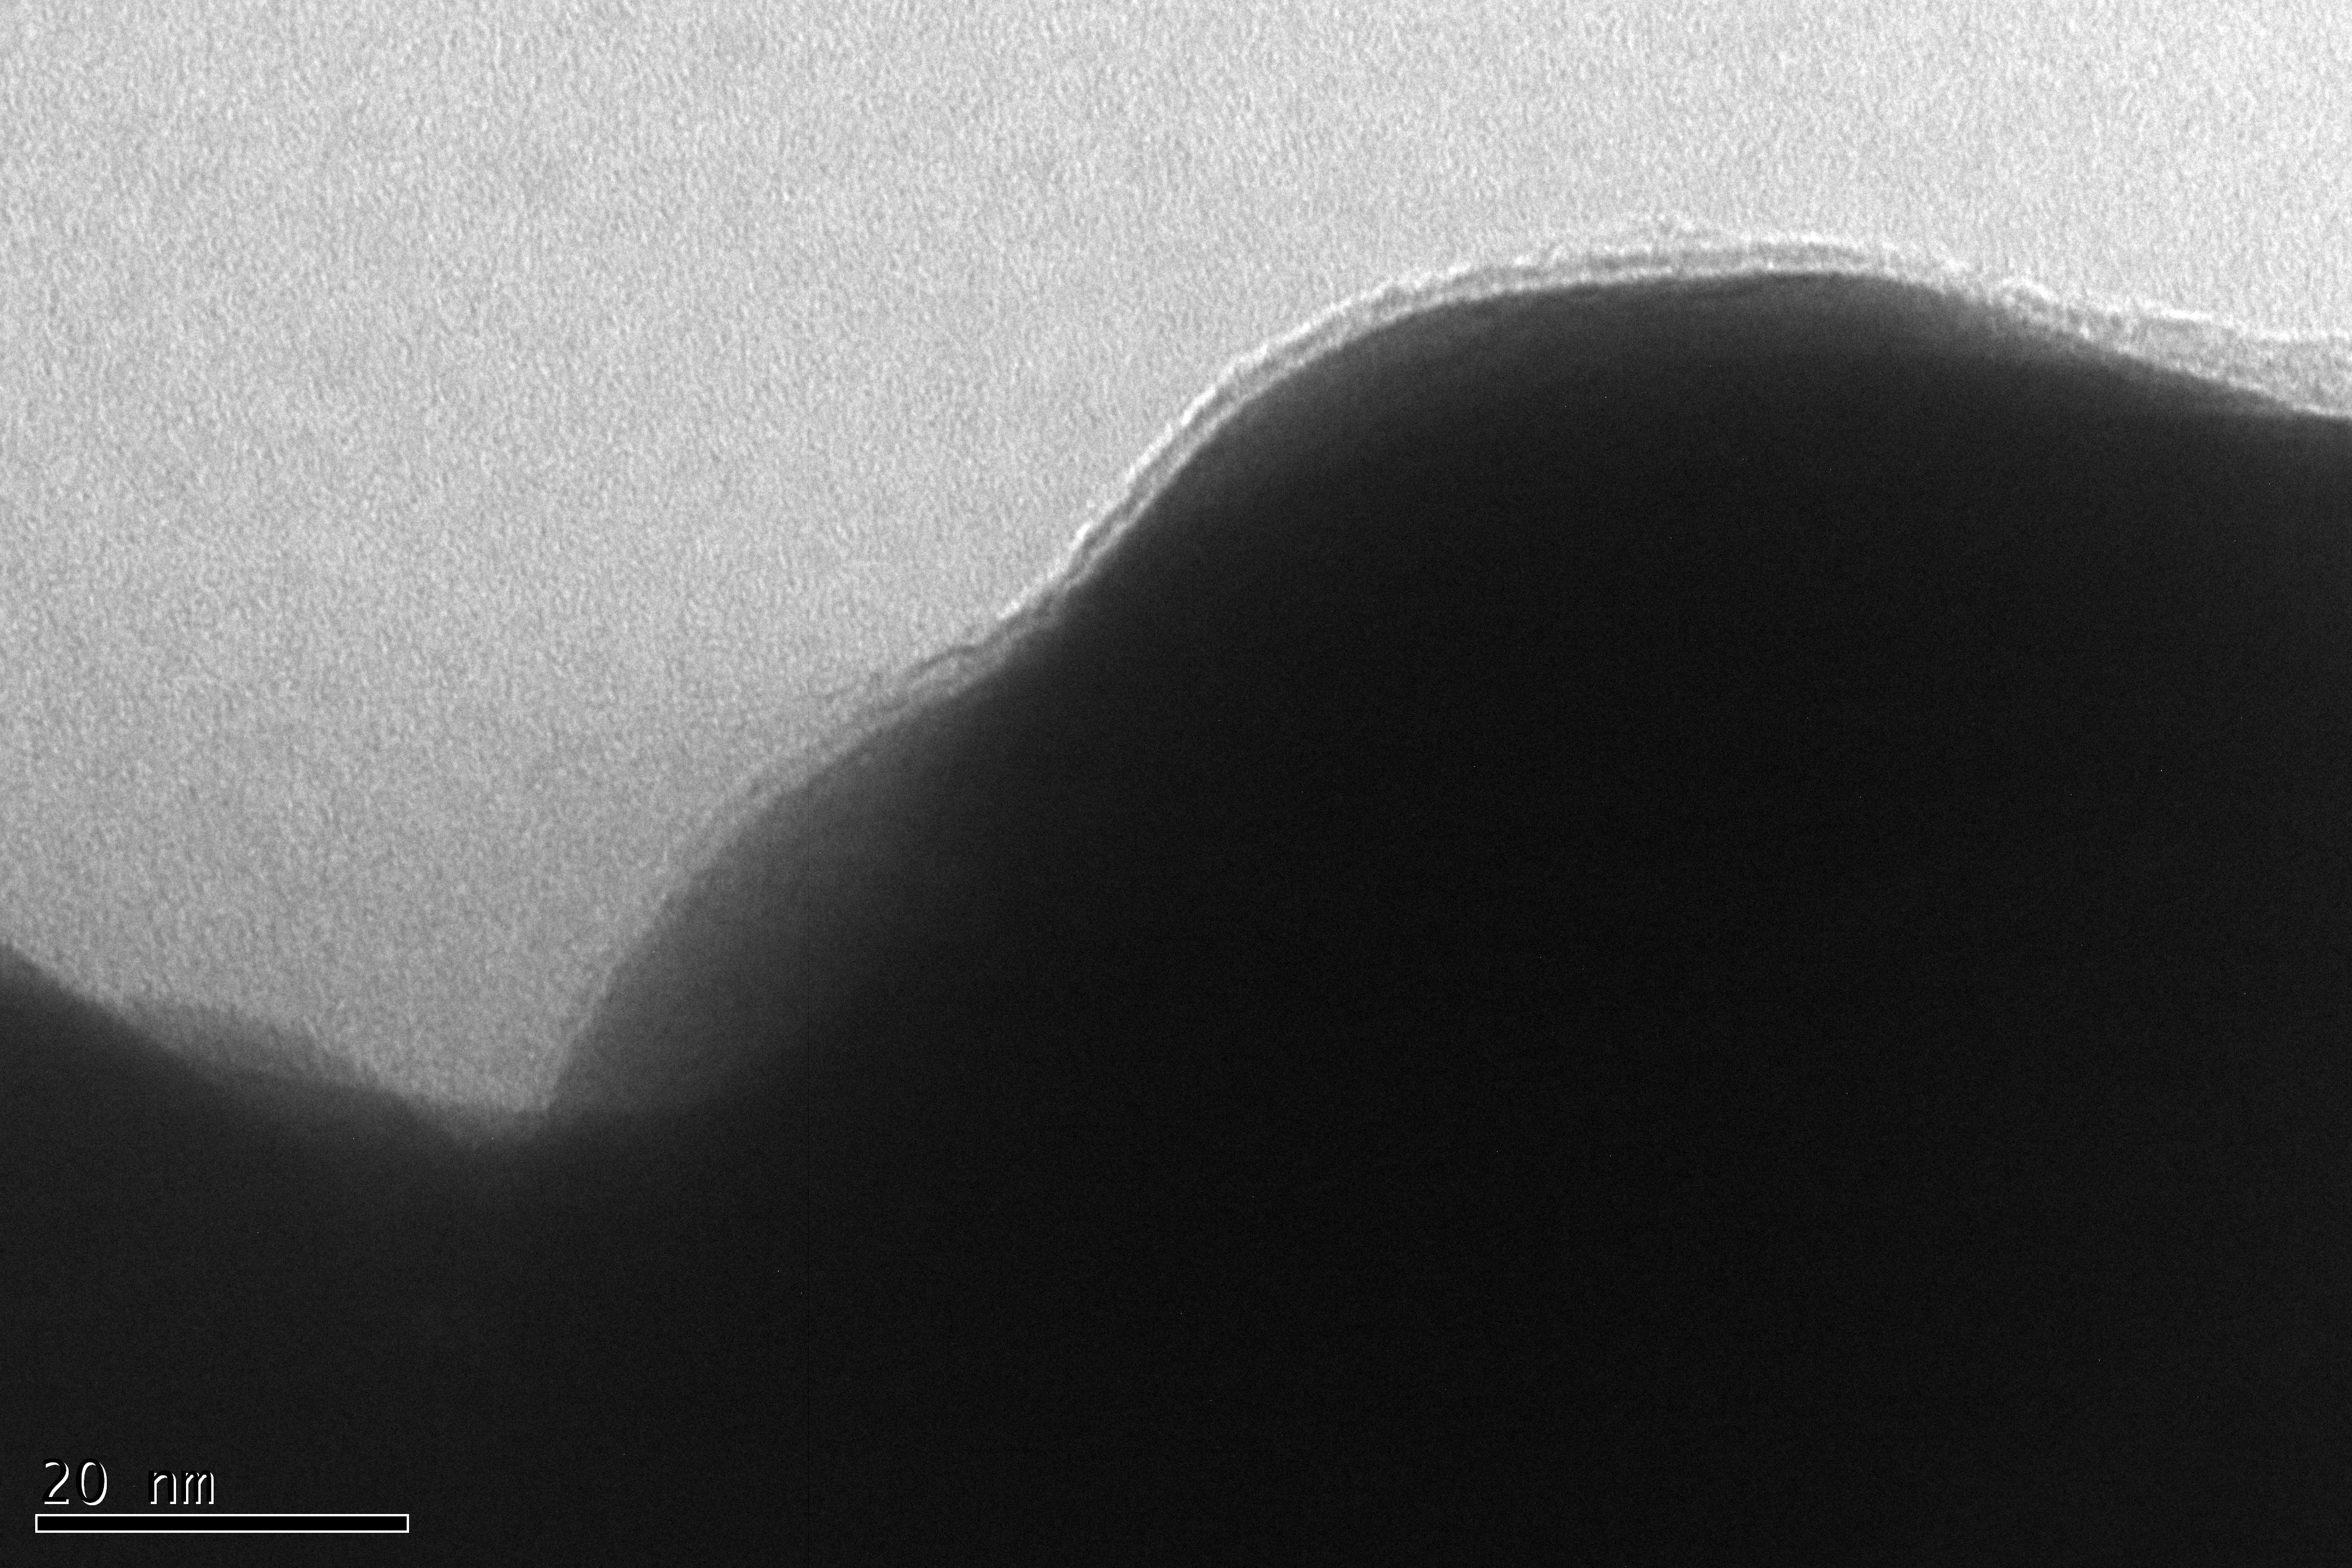
\includegraphics[width=0.33\linewidth]{Bilder/Gel-E-ZnCl-1-1_3}}
			\caption{TEM-Aufnahmen des Gels, das mit \ch{Zn[DDTC]2} und \ch{ZnCl2} im Verhältnis 1:1 \ch{Zn[DDTC]2} zu \ch{ZnCl2} behandelt wurde.}
			\label{fig:Gel-E-ZnCl-1-1}
		\end{figure}
		
		\begin{figure}[H]
			\centering
			\subfloat[\label{fig:Gel-E-ZnCl-1-10_1}]{%
				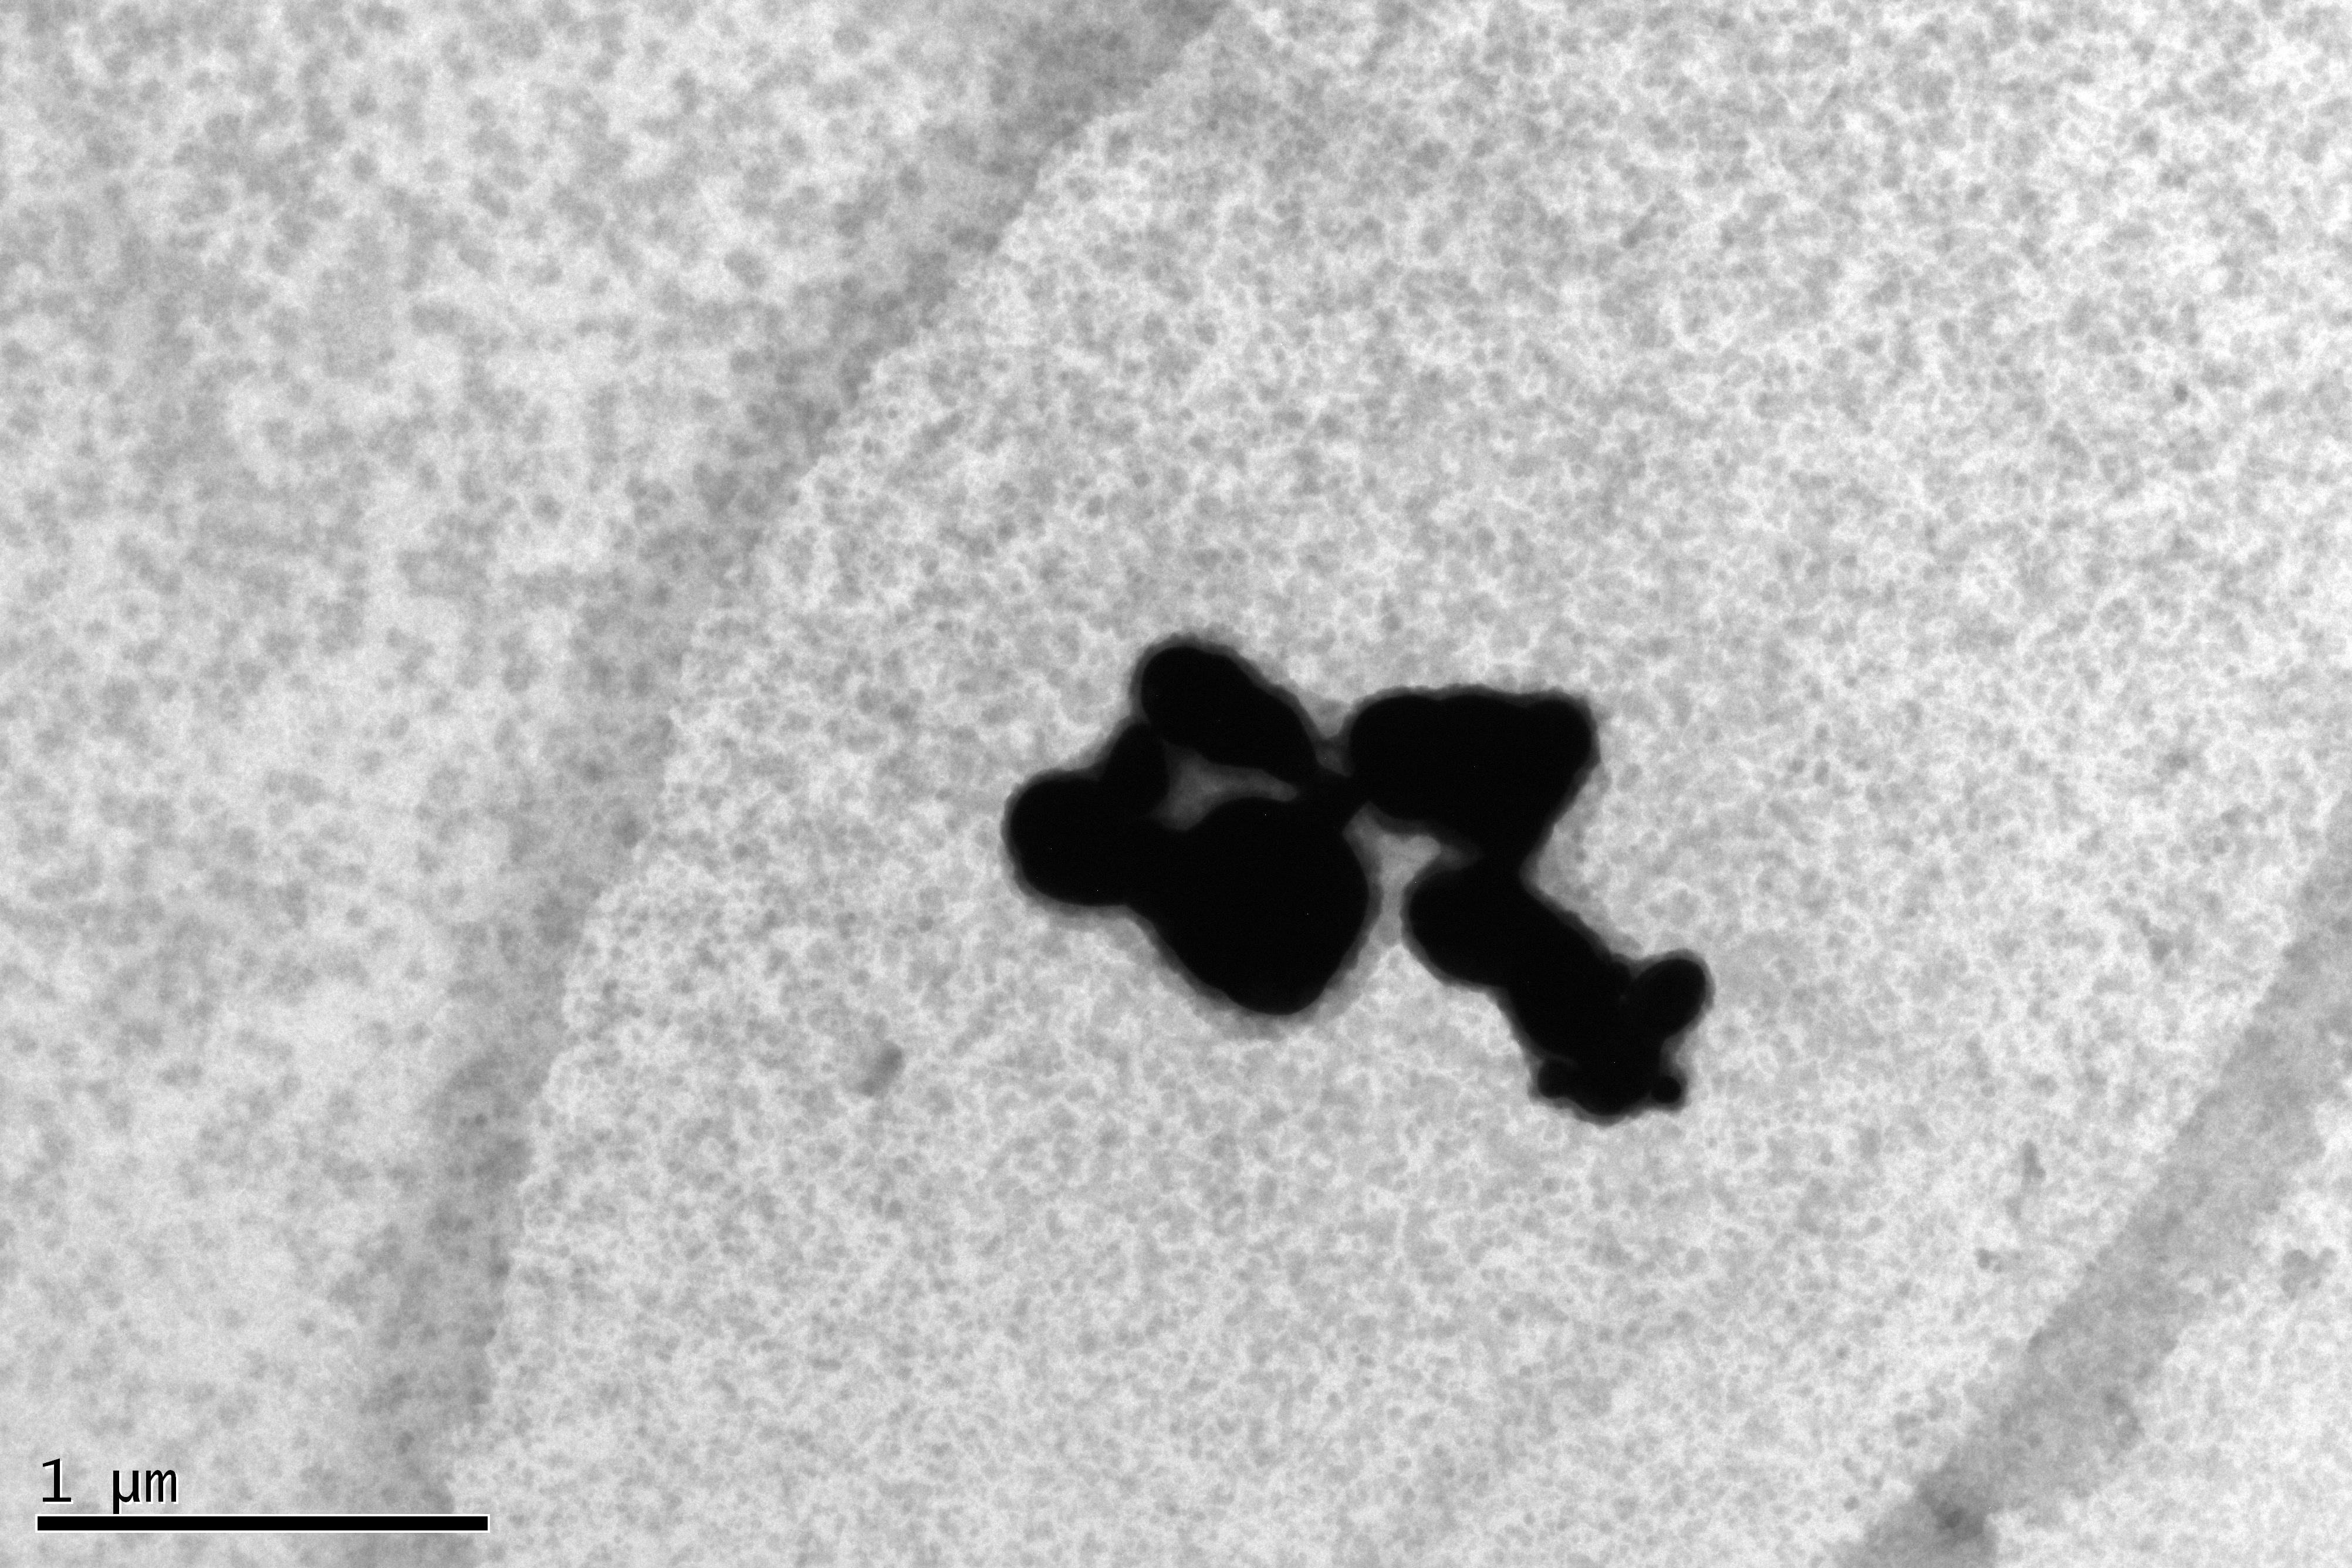
\includegraphics[width=0.33\linewidth]{Bilder/Gel-E-ZnCl-1-10_1}}
			\subfloat[\label{fig:Gel-E-ZnCl-1-10_2}]{%
				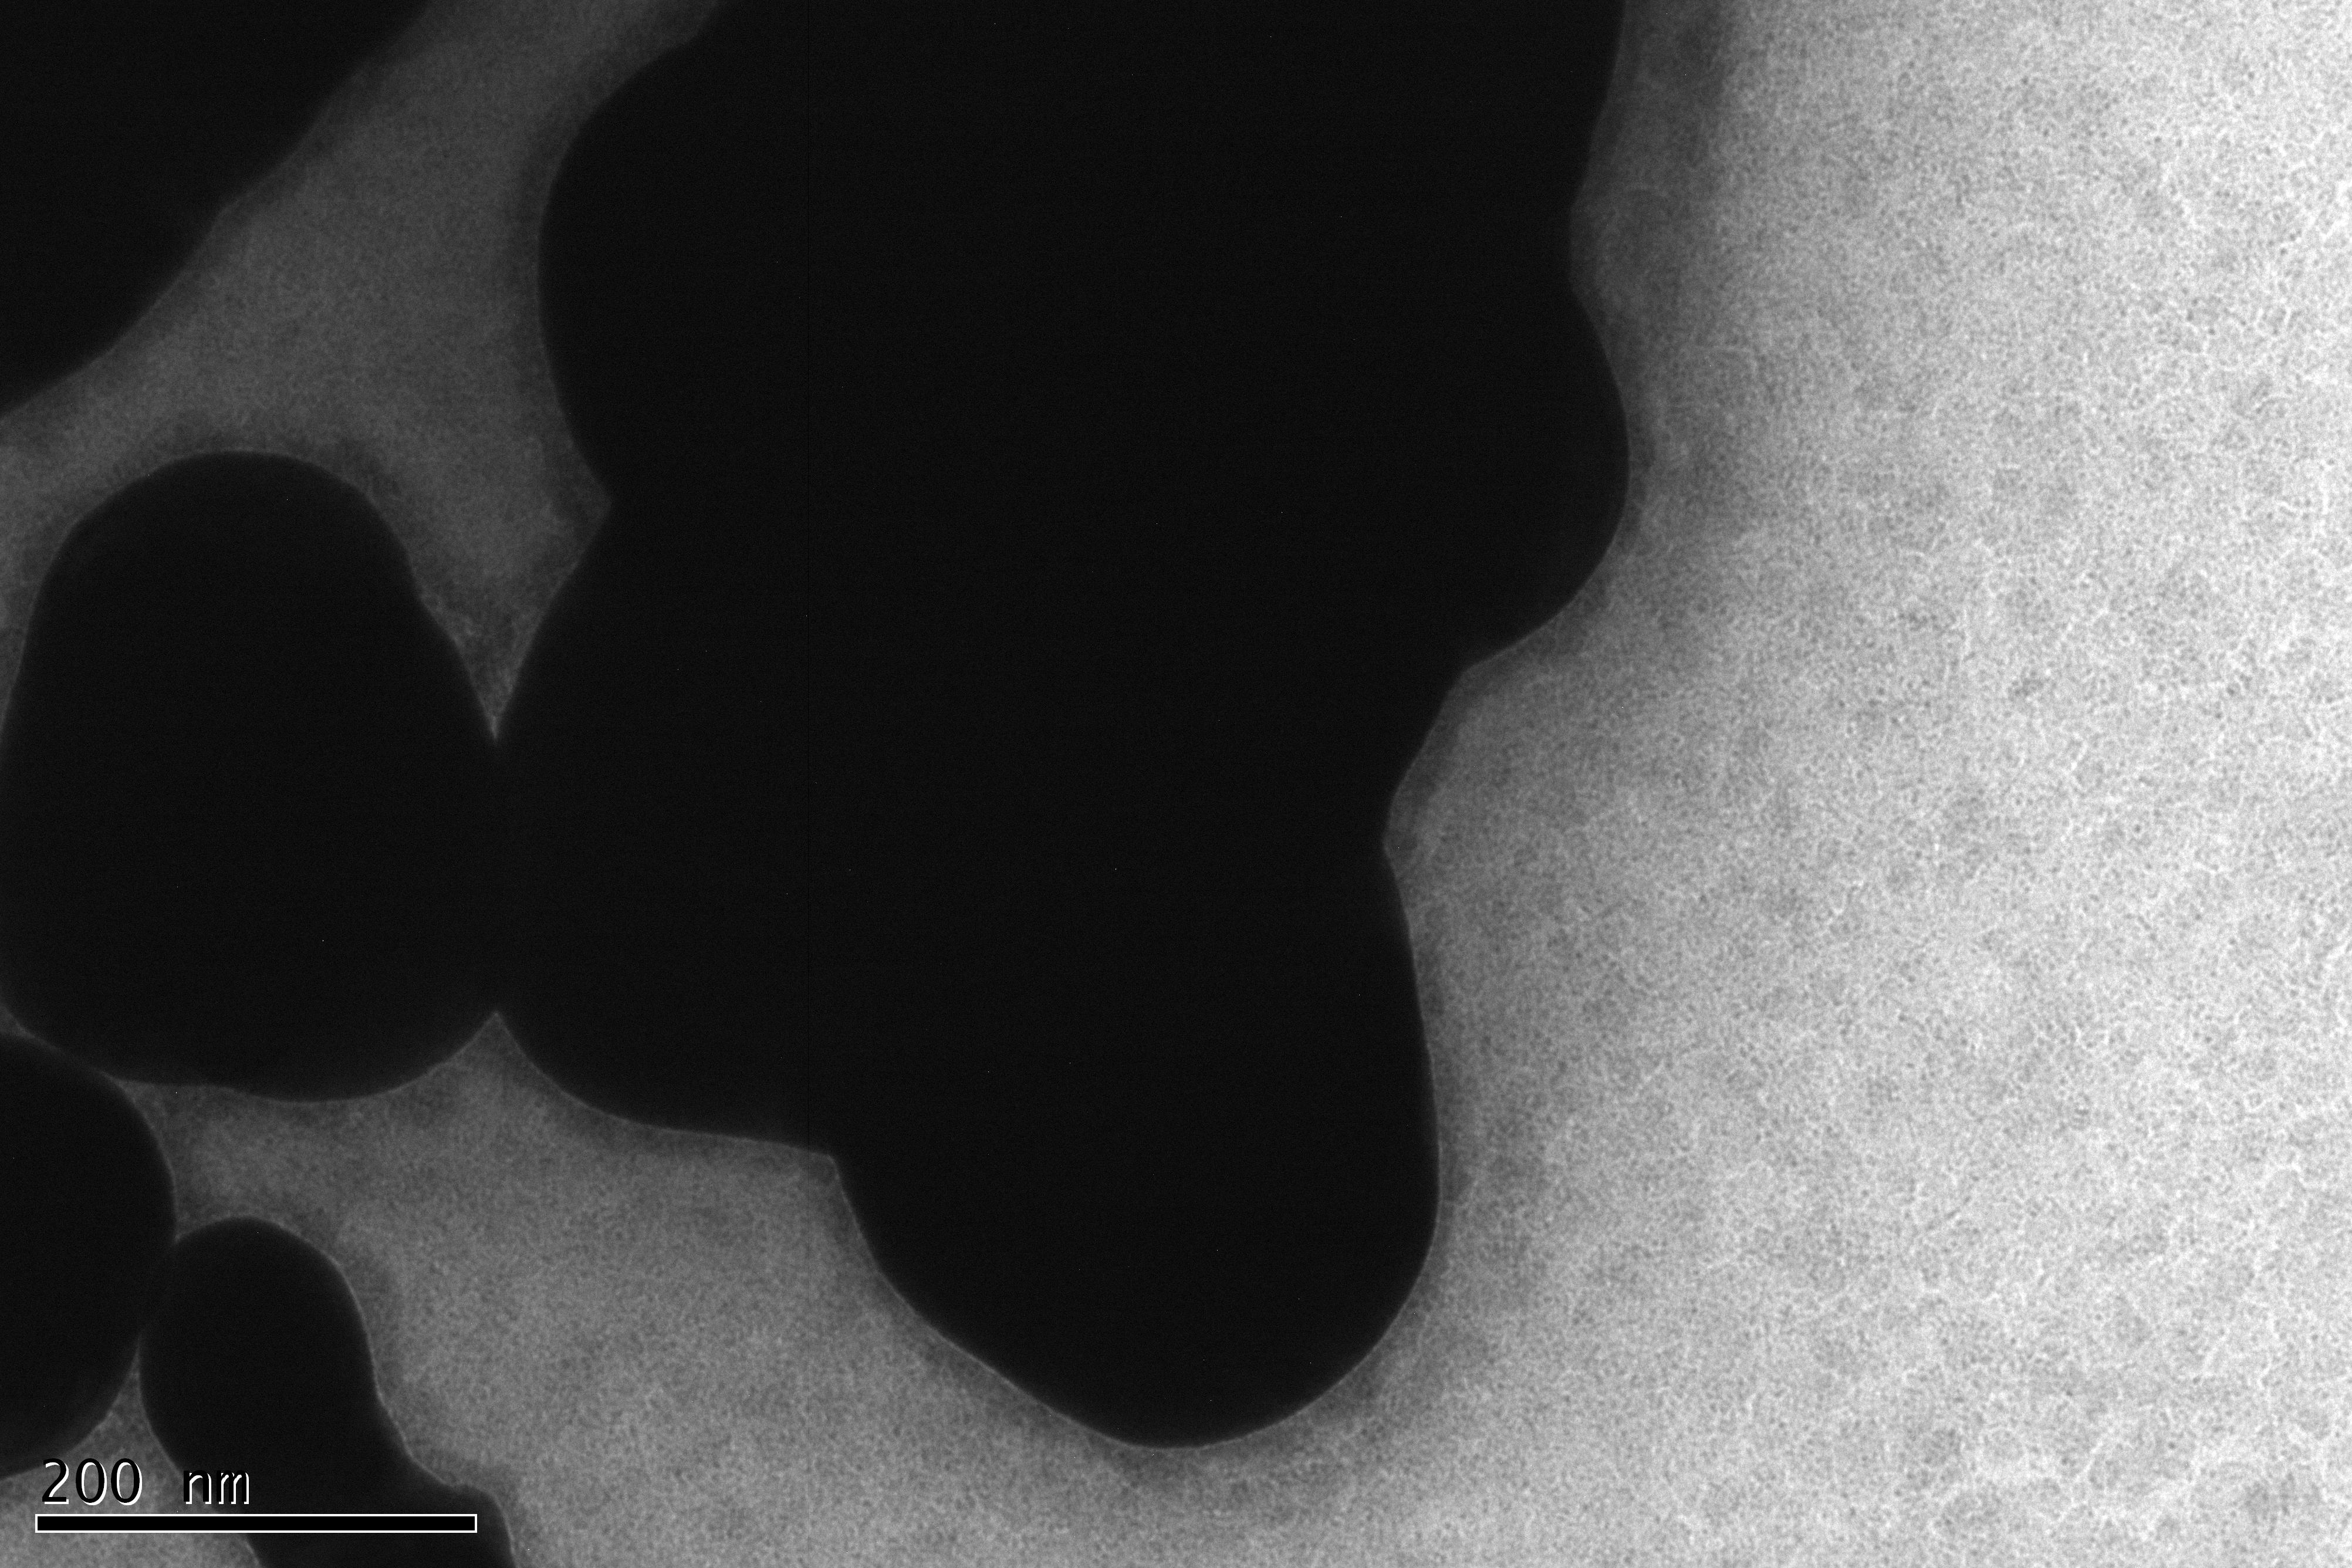
\includegraphics[width=0.33\linewidth]{Bilder/Gel-E-ZnCl-1-10_2}}
			\subfloat[\label{fig:Gel-E-ZnCl-1-10_3}]{%
				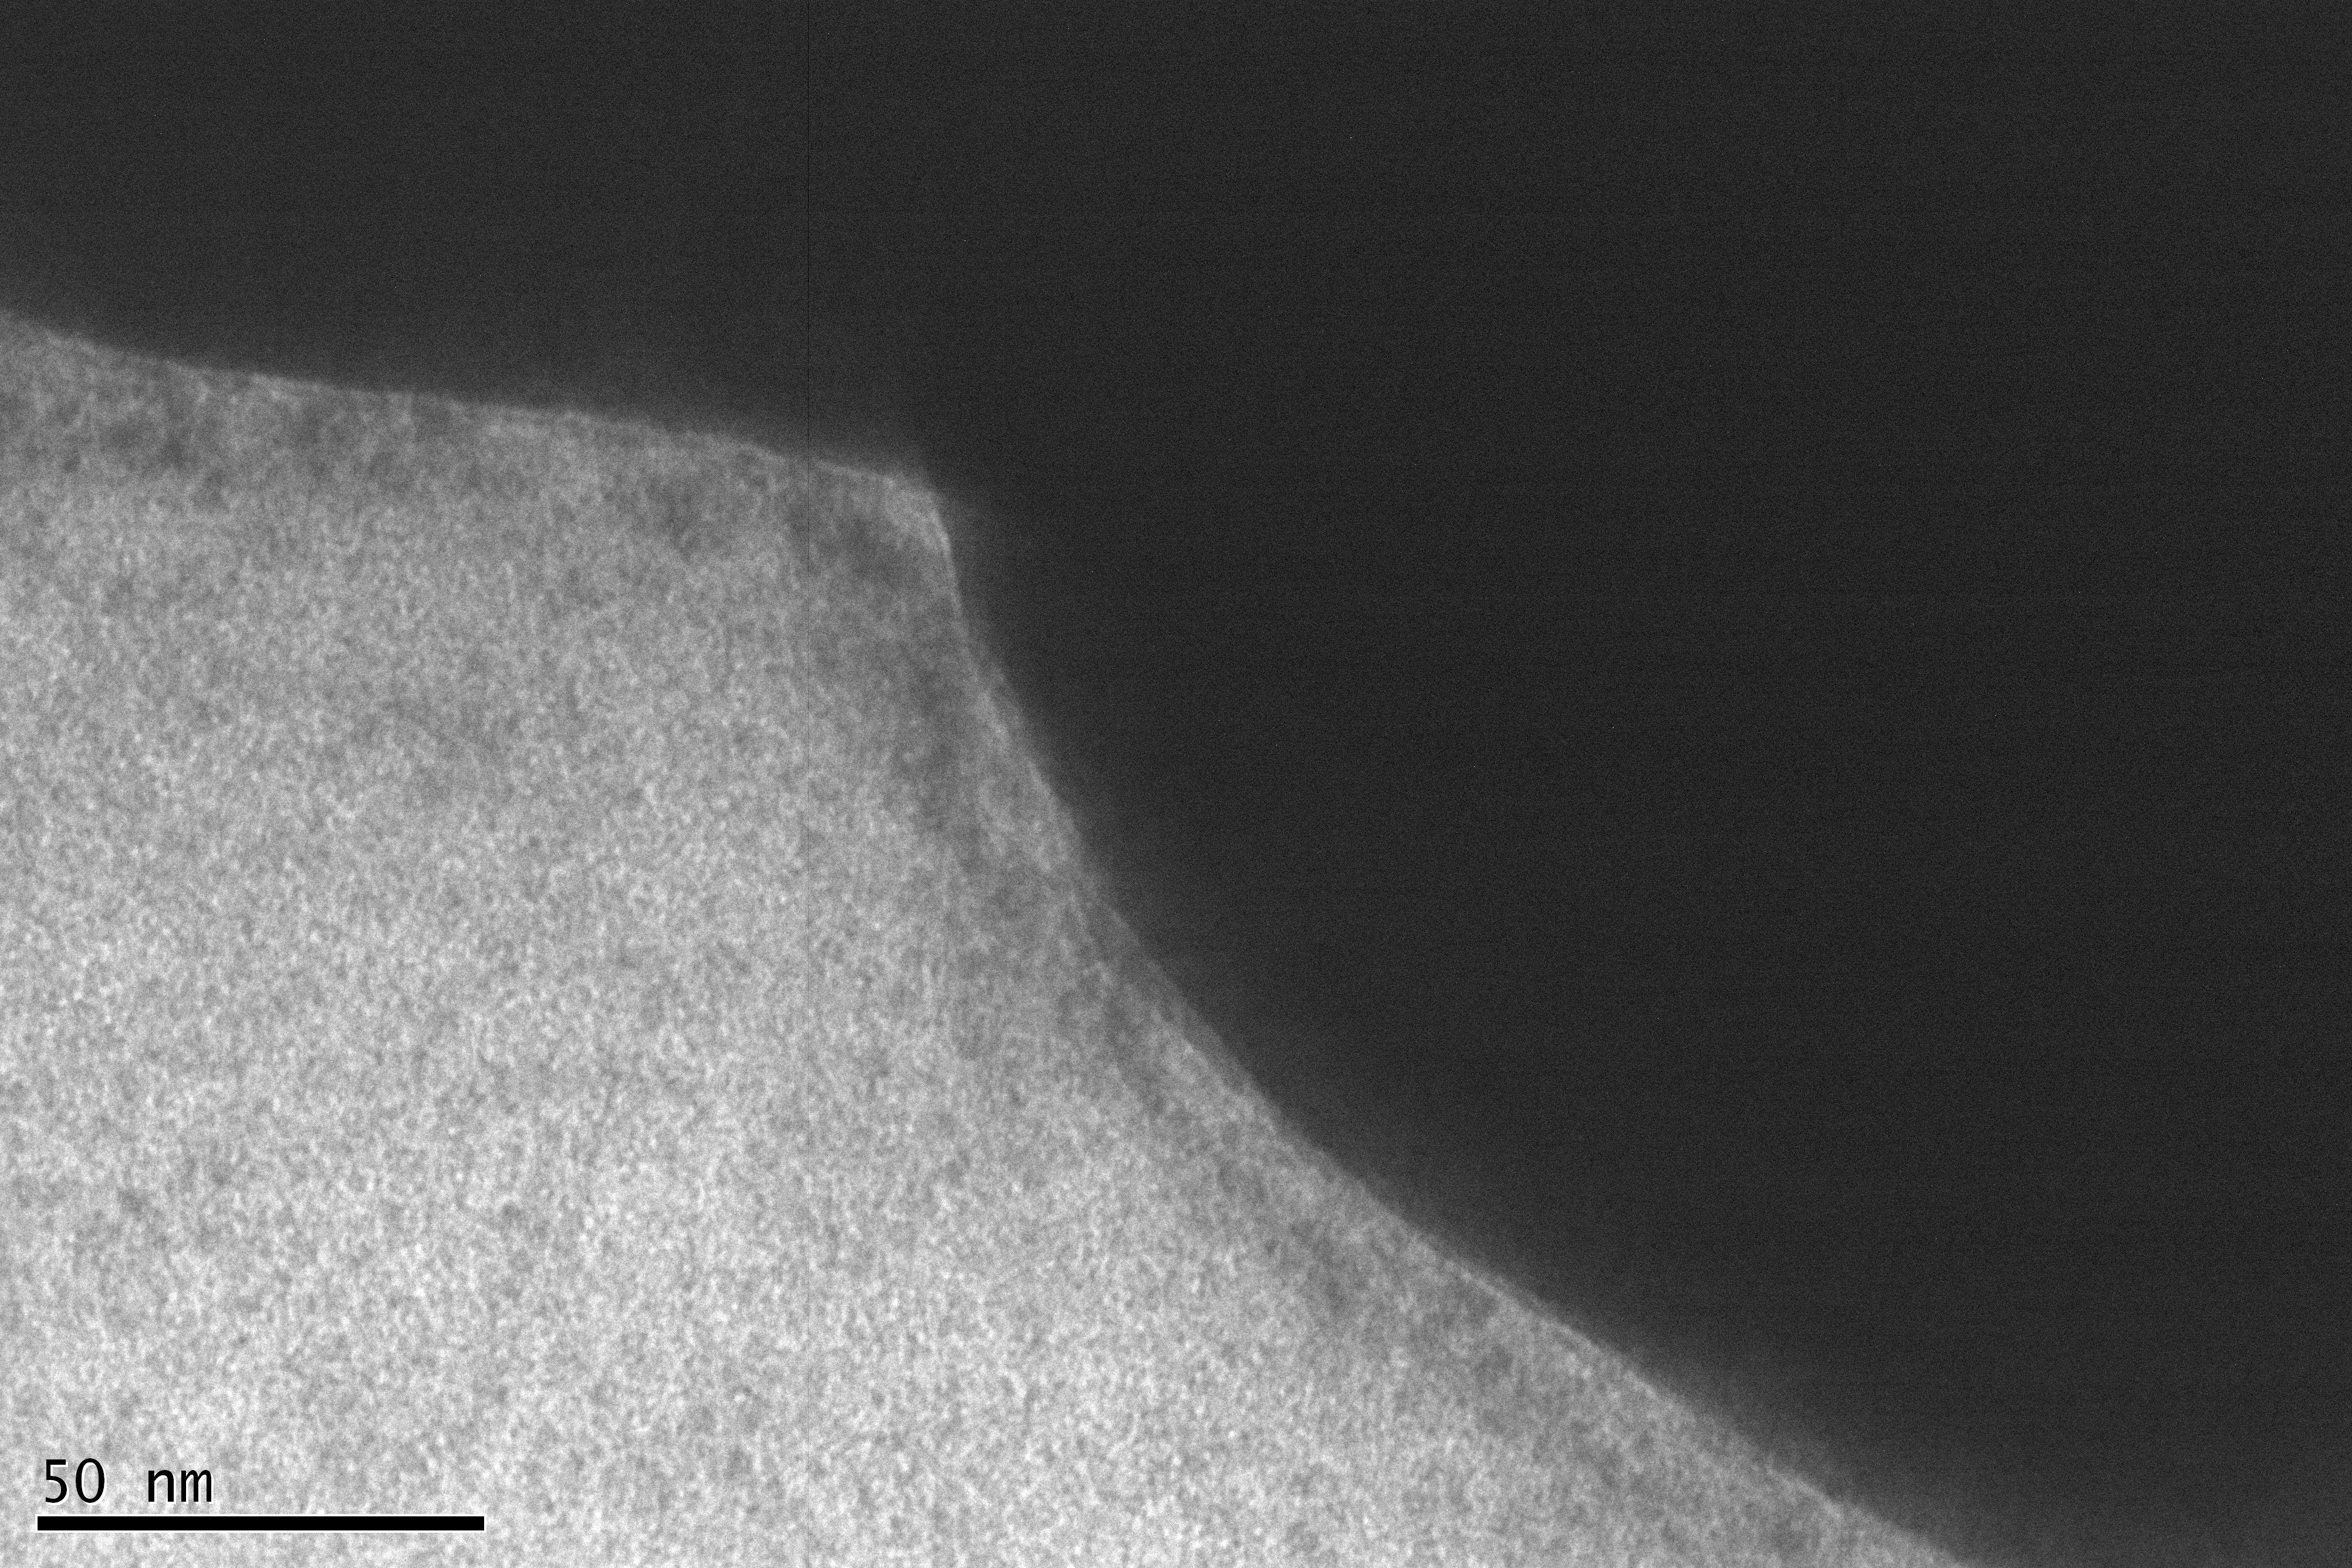
\includegraphics[width=0.33\linewidth]{Bilder/Gel-E-ZnCl-1-10_3}}
			\caption{TEM-Aufnahmen des Gels, das mit \ch{Zn[DDTC]2} und \ch{ZnCl2} im Verhältnis 1:10 \ch{Zn[DDTC]2} zu \ch{ZnCl2} behandelt wurde.}
			\label{fig:Gel-E-ZnCl-1-10}
		\end{figure}
	
		Dieser Effekt konnte allerdings bei der Probe mit dem Verhätnis 1:4 nicht beobachtet werden.
		Hier konnte weder das Bilden einer Schale noch das Aufwachsen einzelner Partikel am Gel beobachtet werden, wie in \cref{fig:Gel-E-ZnCl-1-4} gezeigt ist.
		
		\begin{figure}[H]
			\centering
			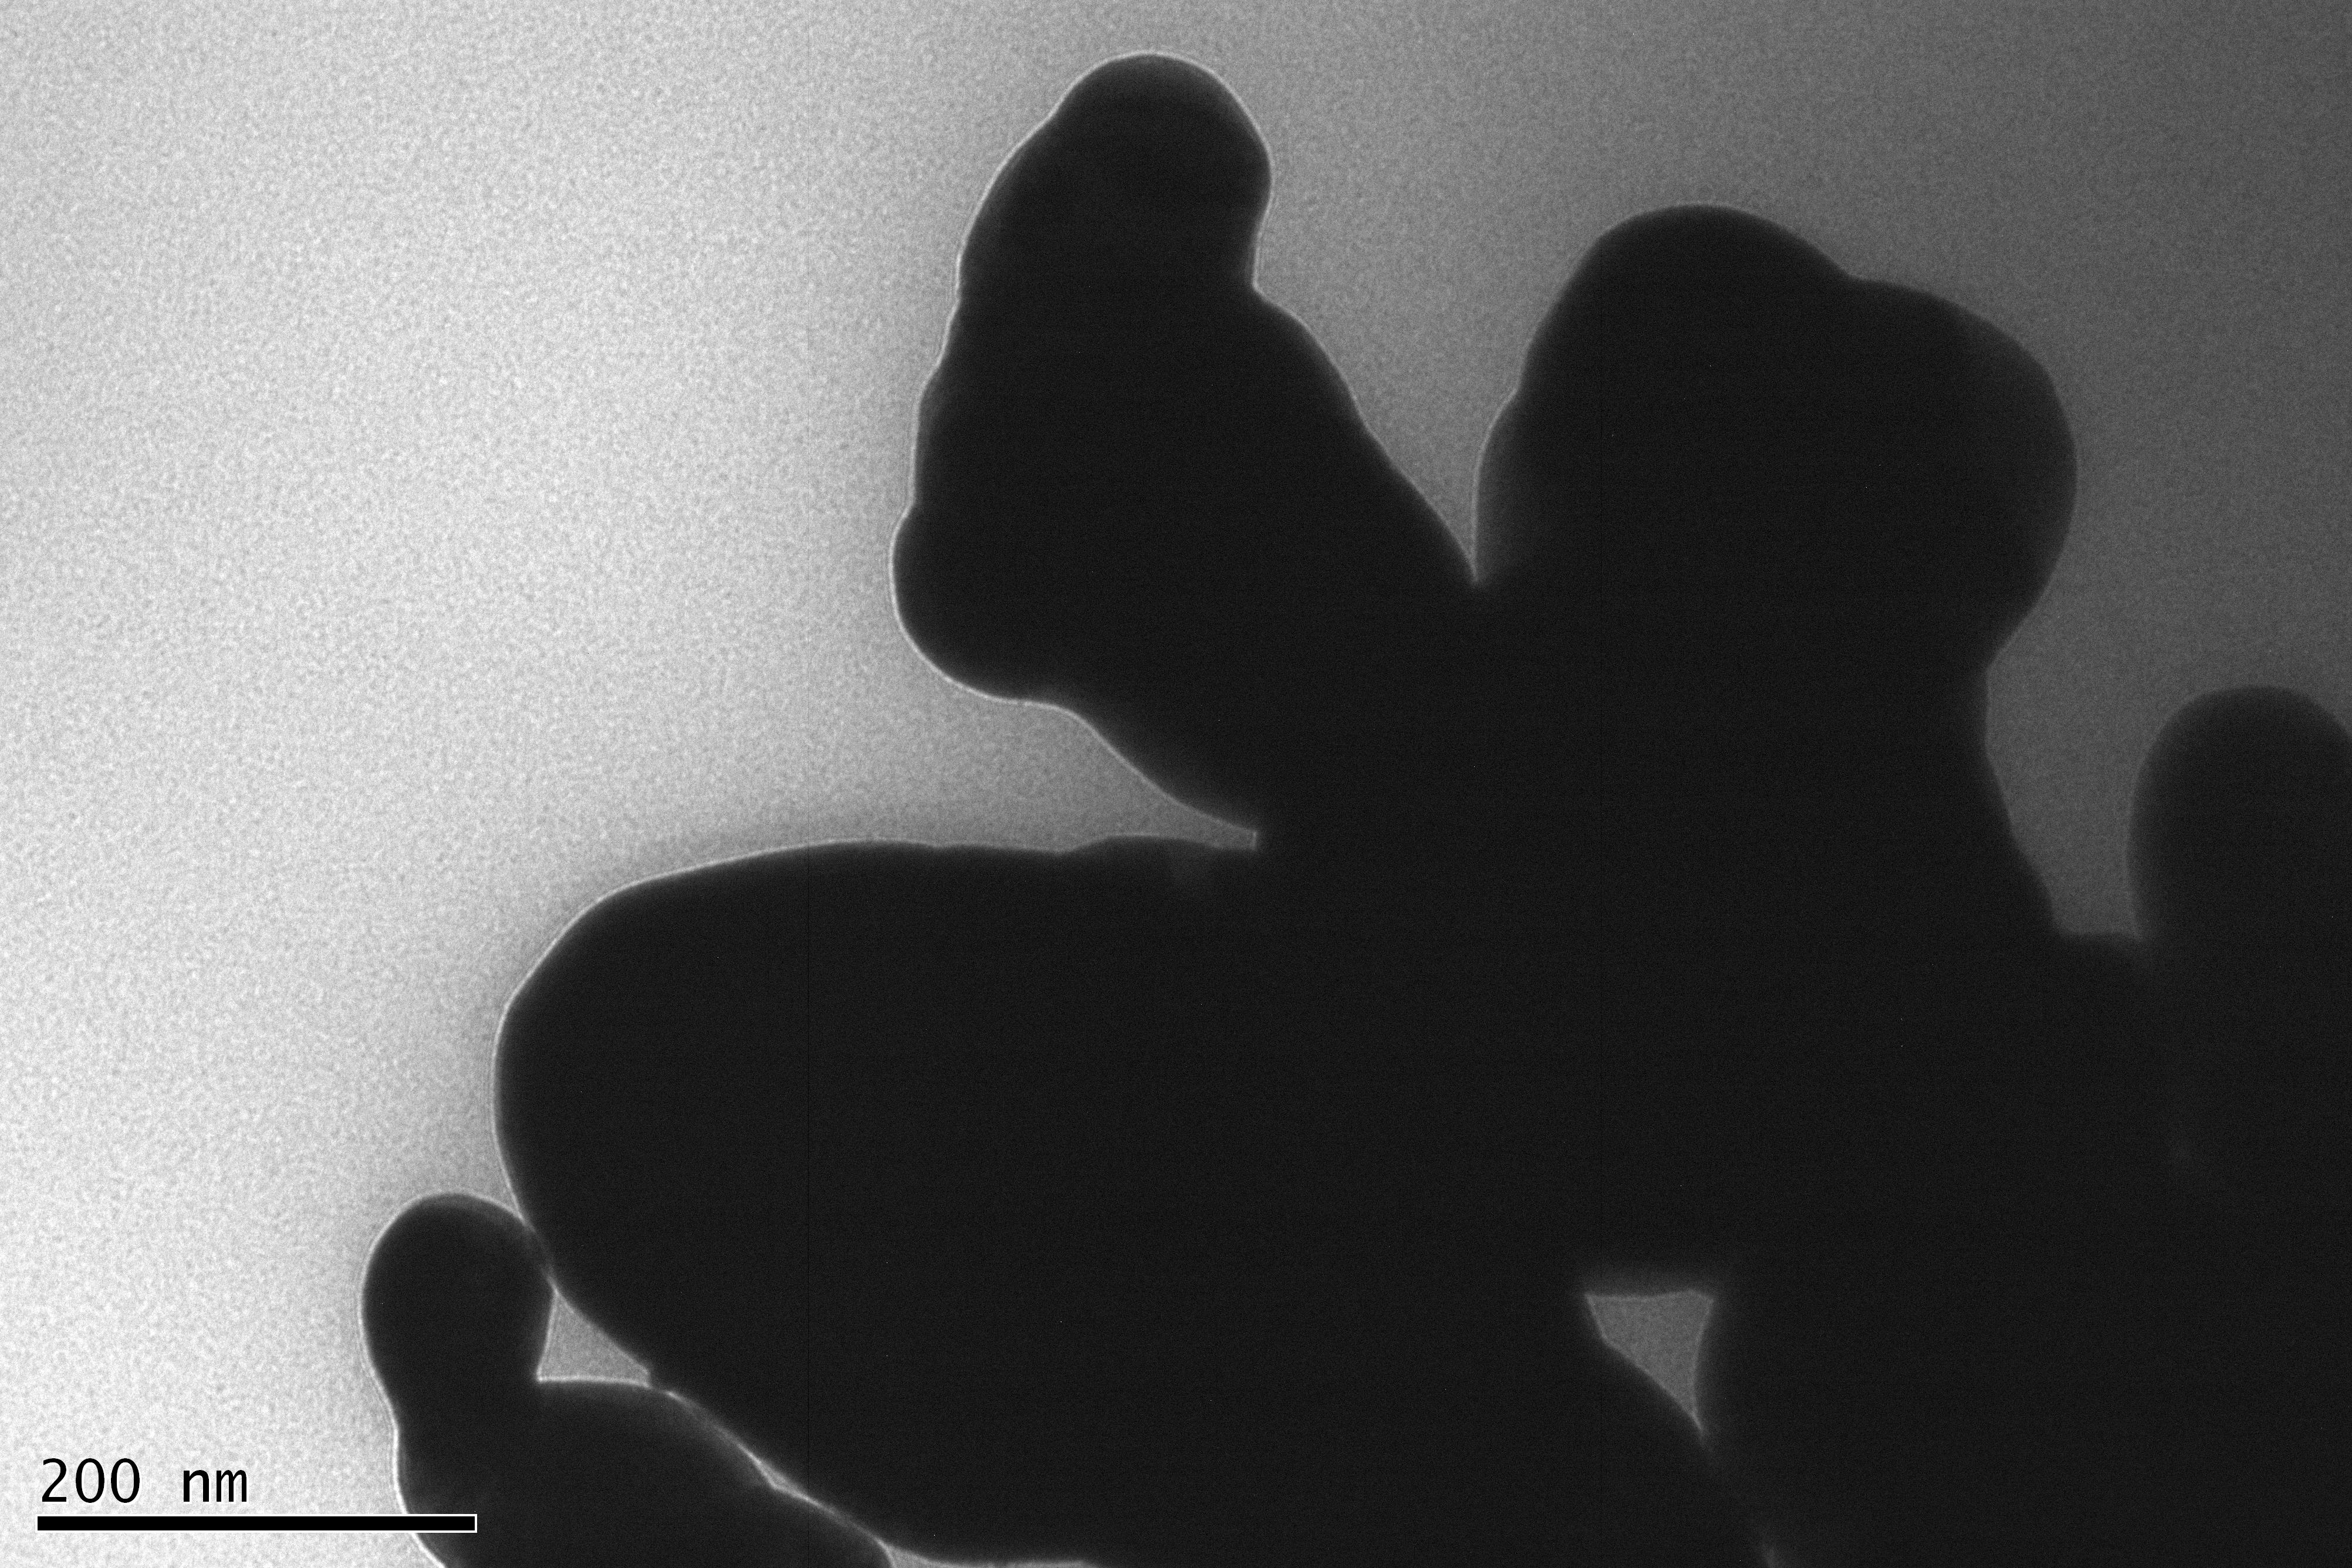
\includegraphics[width=0.6\textwidth]{Bilder/Gel-E-ZnCl-1-4} 	
			\caption{TEM-Aufnahme des Gels, das mit \ch{Zn[DDTC]2} und \ch{ZnCl2} im Verhältnis 1:4 \ch{Zn[DDTC]2} zu \ch{ZnCl2} behandelt wurde.}
			\label{fig:Gel-E-ZnCl-1-4}
		\end{figure}
	
		\subsubsection{Variation der Konzentration}
		Da bei den Versuchen häufig ein Großteil der gebildeten Partikel neben den Gelen vorlag, wurden Reaktionen mit Lösungen mit geringeren Konzentrationen an \ch{Cd[DDTC]2} und \ch{CdCl2} untersucht.
		Bei der Probe mit 0,05~M \ch{Cd[DDTC]2}-Lösung, deren TEM-Messung in \cref{fig:Gel-E-CdS-0-05} dargestellt ist,  zeigt sich ein ähnliches Bild wie bei den Proben mit 0,11~M.
		Es bilden sich viele Partikel , die sich um das Gel herum anlagern, allerdings ist auch hier die Menge an CdS Partikel, die neben dem Gel liegen hoch.
		Eine deutlichere Änderung lässt sich bei der Probe mit 0,01~M \ch{Cd[DDTC]2}-Lösung beobachten, wie \cref{fig:Gel-E-CdS-0-01} zeigt.
		Hier konnten keine CdS-Partikel gefunden werden, die neben dem Gel vorlagen.
		An den Gelen selbst ist eine kleine Schicht CdS zu erkennen.
		Durch die Konzentrationsänderung konnte das Nukleationsverhalten also so angepasst werden, dass sich das CdS am Gel gebildet hat.
		
		\begin{figure}[H]
			\centering
			\includegraphics[width=0.6\textwidth]{Bilder/Gel-E-CdS-0,05} 	
			\caption{TEM-Aufnahme des Gels, das mit 0,05M \ch{Cd[DDTC]2}-Lösung behandelt wurde.}
			\label{fig:Gel-E-CdS-0-05}
		\end{figure}
	
		\begin{figure}[H]
			\centering
			\includegraphics[width=0.6\textwidth]{Bilder/Gel-E-CdS-0,01} 	
			\caption{TEM-Aufnahme des Gels, das mit 0,01M \ch{Cd[DDTC]2}-Lösung behandelt wurde.}
			\label{fig:Gel-E-CdS-0-01}
		\end{figure}
		
		Es wurde auch nochmal der Einfluss von  0,05~M \ch{CdCl2}-Lösung mit einer  0,05~M \ch{Cd[DDTC]2}-Lösung untersucht.
		Hierbei zeigte sich ein ähnliches Bild wie bei den untersuchten Gelen die mit 0,11~M-Lösungen behandelt wurden.
		Sowohl beim  \ch{Cd[DDTC]2}:\ch{CdCl2} Verhältnis 1:1 (\cref{fig:Gel-E-CdCl-1-1-0-05}) als auch 1:4 (\cref{fig:Gel-E-CdCl-1-4-0-05}) als auch 1:10 (\cref{fig:Gel-E-CdCl-1-10-0-05}), konnte die Bildung von CdS beobachtet werden.
		Dieses liegt zu einem Großteil wieder neben den Gelen vor, wie auch schon bei den vorherigen Proben mit gleichen Verhältnissen mit 0,11~M-Lösungen.
		
		\begin{figure}[H]
			\centering
			\includegraphics[width=0.6\textwidth]{Bilder/Gel-E-CdCl-1-1-0,05} 	
			\caption{TEM-Aufnahme des Gels, das mit \ch{Cd[DDTC]2} und \ch{CdCl2} im Verhältnis 1:1 \ch{Cd[DDTC]2} zu \ch{CdCl2} mit einer Konzentration von 0,05~M behandelt wurde.}
			\label{fig:Gel-E-CdCl-1-1-0-05}
		\end{figure}
		
		\begin{figure}[H]
			\centering
			\includegraphics[width=0.6\textwidth]{Bilder/Gel-E-CdCl-1-4-0,05} 	
			\caption{TEM-Aufnahme des Gels, das mit \ch{Cd[DDTC]2} und \ch{CdCl2} im Verhältnis 1:4 \ch{Cd[DDTC]2} zu \ch{CdCl2} mit einer Konzentration von 0,05~M behandelt wurde.}
			\label{fig:Gel-E-CdCl-1-4-0-05}
		\end{figure}
	
		\begin{figure}[H]
			\centering
			\includegraphics[width=0.6\textwidth]{Bilder/Gel-E-CdCl-1-10-0,05} 	
			\caption{TEM-Aufnahme des Gels, das mit \ch{Cd[DDTC]2} und \ch{CdCl2} im Verhältnis 1:10 \ch{Cd[DDTC]2} zu \ch{CdCl2} mit einer Konzentration von 0,05~M behandelt wurde.}
			\label{fig:Gel-E-CdCl-1-10-0-05}
		\end{figure}
		
	\subsubsection{Variation des Gels}
		Bislang wurden alle Experimente an gleichen Gelen vorgenommen.
		Aus diesem Grund wurde eine Probe mit den Bi-metallischen Au/Ag-Gelen durchgeführt.
		Beim Stufenweisen Austausch der flüssigen Phase der Gele schrumften diese merklich, wie in \cref{fig:Foto-Gel-cit} gezeigt ist.
		Auf dem Foto ist das Gel nach dem Austausch zu sehen. 
		Da kleine Teile des Gels sich am Rand des Gefäßes anhafteten,  kann man daran die Größe der Gele vor dem Austausch gut erkennen. 
		Das resultierende Volumen des Gels nach dem Austausch war etwa ein Drittel vom Ausgangsvolumen.
		Teile der Poren scheinen also während des Austausches der flüssigen Phase kollabiert zu sein.
		
		\begin{figure}[H]
			\centering
			\includegraphics[width=0.6\textwidth]{Bilder/Foto-Gel-cit} 	
			\caption{Bild vom bi-metallischen Au/Ag-Gel nach dem Austausch der flüssigen Phase.}
			\label{fig:Foto-Gel-cit}
		\end{figure}
	
		Die Probe mit dem bi-metallischen Au/Ag-Gel zeigt nach Behandlung mit der 0,11~M \ch{Cd[DDTC]2}-Lösung ein ähnliches Bild wie die vorher verwendeten Gele, wie in \cref{fig:Gel-C-CdS} gezeigt.
		Auch hier bildet sich wieder ein Teil des CdS neben dem Gel.
		Es ist jedoch auch eine kleine Schicht an den Gelen zu erkennen, was in \cref{fig:Gel-C-CdS_2} deutlich zu sehen ist.
		Es konnte also auch an diesem Gel nachträglich CdS aufgewachsen werden.
		
		\begin{figure}[H]
			\centering
			\subfloat[\label{fig:Gel-C-CdS_1}]{%
				\includegraphics[width=0.45\linewidth]{Bilder/Gel-C-CdS_1}}
			\subfloat[\label{fig:Gel-C-CdS_2}]{%
				\includegraphics[width=0.45\linewidth]{Bilder/Gel-C-CdS_2}}
			\caption{TEM-Bilder des bi-metallischen Au/Ag-Gel nach Behandlung mit 0,11~M \ch{Cd[DDTC]2}-Lösung.}
			\label{fig:Gel-C-CdS}
		\end{figure}
		
		 
		
		
		
		
	   
	
 
 